% $Header: /cvsroot/latex-beamer/latex-beamer/solutions/generic-talks/generic-ornate-15min-45min.en.tex,v 1.4 2004/10/07 20:53:08 tantau Exp $

%\documentclass[10pt,xcolor,dvipssnames,table,handout]{beamer}
\documentclass[10pt,xcolor,dvipssnames,table]{beamer}
%\usepackage[pdftex]{graphicx}
\usepackage[update]{epstopdf}

\mode<presentation>
{
%  \usetheme{Malmoe}
  \usetheme{Copenhagen}
  \useoutertheme{infolines}
%  \usetheme{Warsaw}
  % or ...

  \setbeamercovered{transparent}
%  \setbeamercovered{dynamic}
  % or whatever (possibly just delete it)
\setbeamercolor{alerted text}{fg=blue!80!black}
% doesnt work:
%\addfootbox{structure}{\tiny \FileName}
}

\mode<handout>
{
  \usetheme{Malmoe}
% No footline on title slide
\setbeamertemplate{footline}[page number]
%\defbeamertemplate{footline}{title slide}{%
%	\relax
%}
\setbeamertemplate{footline}[title slide]
}

%%% Customizations
\setbeamertemplate{items}[ball]
\setbeamercolor{subitem projected}{bg=red}
%\setbeamercolor{itemize subitem}{fg=red}
% remove navigation symbols
\setbeamertemplate{navigation symbols}{}

%% No footline on title slide
% \defbeamertemplate{footline}{title slide}{%
% 	\relax
% }
% \setbeamertemplate{footline}[title slide]

% \setbeamertemplate{title page}
% {
% \begin{centering}
%  {\usebeamerfont{title}\usebeamercolor[fg]{title}\inserttitle} \\
%  {\usebeamerfont{subtitle}\usebeamercolor[fg]{subtitle}\insertsubtitle}
% \end{centering}
% 
% }

\newcommand{\FileName}{}
%\addtobeamertemplate{footline}{\tiny\FileName\hfill}{}
%\setbeamertemplate{footline}{page number}
%{%
%  \FileName%
%  \hfill%
%  \usebeamercolor[fg]{page number in head/foot}%
%  \usebeamerfont{page number in head/foot}%
%  \insertpagenumber\,/\,\insertpresentationendpage\kern1em\vskip2pt%
%}
%%

\vfuzz=8pt

\usepackage[comma]{natbib}
\bibliographystyle{abbrvnat-last}

%\usepackage[latin1]{inputenc}
% or whatever

\usepackage{comment}
\usepackage{times}
\usepackage{mdwlist}
\usepackage{xcolor}
\usepackage{bm}
\usepackage{sasnames}
\usepackage{multirow}
\usepackage{Sweave}

\hypersetup{bookmarksopenlevel=2}
%\usepackage{multimedia}


%% Definitions and environments for vcdframes

% references
\newcommand*{\sref}[1]{Slide \ref{#1}}
\newcommand*{\figref}[1]{Figure~\ref{#1}}
\newcommand*{\tabref}[1]{Table~\ref{#1}}

% colors
\newcommand*{\red}[1]{{\color{red}#1}}
\newcommand*{\blue}[1]{{\color{blue}#1}}
\newcommand*{\black}[1]{{\color{black}#1}}
\newcommand*{\green}[1]{{\color{green}#1}}
\newcommand*{\yellow}[1]{{\color{yellow}#1}}
\newcommand*{\gold}[1]{{\color{yellow!50!orange}#1}}
%\newcommand*{\yellow}[1]{\fcolorbox{gray}{black}{\color{yellow}#1}}
\newcommand*{\yellowbg}[1]{\fcolorbox{gray}{yellow}{#1}}
%\newcommand*{\yellow}[1]{{\color{yellow}#1}}
\newcommand*{\purple}[1]{{\color{purple}#1}}

% SAS - examples
  \renewcommand{\macro}[1]{\texttt{\structure{#1}} macro}
  \newcommand{\macrot}[1]{\texttt{#1} macro}
  \newcommand*{\sasprog}[1]{\texttt{\structure{#1}} program}
  \newcommand*{\sasprogt}[1]{\texttt{#1} program}
  \newcommand*{\sascomment}[1]{\textit{\red{#1}}}
  \newcommand*{\sasemph}[1]{\textbf{\blue{#1}}}

% R
\newcommand*{\pkg}[1]{\texttt{#1} package}
%\newcommand{\func}[1]{\texttt{#1()}}
\newcommand*{\code}[1]{{\texttt{\blue{#1}}}}
\newcommand*{\func}[1]{{\texttt{\purple{#1()}}}}

\renewcommand{\proc}[1]{\texttt{#1}}
%\newcommand*{\sasprogt}[1]{\textsc{#1} program}
\newcommand{\IX}[1]{#1}
\renewcommand{\stmt}[1]{\texttt{#1} statement}
\renewcommand*{\pname}[1]{\texttt{\blue{\MakeUppercase{#1}}}}

\newcommand {\VCD}{\textit{\textsf{VCD}}}
\newcommand{\vcdstory}[1]{/home/friendly/Library/Documents/tex/vcdstory/fig/#1}
\newcommand{\vcdguide}[1]{/home/friendly/Library/Documents/tex/vcdguide/fig/#1}
\newcommand{\gsaseps}[1]{/home/friendly/sasuser/catdata/grcat/#1}

% Math stuff
\newcommand*{\given}{\ensuremath{\, | \,}}
\renewcommand*{\vec}[1]{\ensuremath{\bm{#1}}}
\newcommand{\mat}[1]{\ensuremath{\bm{#1}}}
\newcommand{\trans}{\ensuremath{^\mathsf{T}}}
\newcommand{\diag}[1]{\ensuremath{\mathrm{diag} (#1)}}
%\def\binom#1#2{{#1 \choose #2}}%
\renewcommand{\implies}{ \ensuremath{\mapsto} }
\newcommand*{\dev}[1]{(#1 - \bar{#1})}
\renewcommand*{\det}[1]{\mathrm{det}(#1)}
\newcommand*{\inv}[1]{\ensuremath{\mat{#1}^{-1}}}
\newcommand*{\half}[1]{\ensuremath{\mat{#1}^{1/2}}}
\newcommand*{\nvec}[2]{\ensuremath{{#1}_{1}, {#1}_{2},\ldots,{#1}_{#2}}}
\newcommand*{\period}{\:\: .}
\newcommand*{\comma}{\:\: ,}

\renewcommand{\emph}[1]{\alert{\textit{#1}}}
\renewcommand{\nway} {\textit{n}-way}
\newcommand{\ignore}[1]{}
%\includecoment{fullversion}

\let\proglang=\textsf
\let\dispwidth=\textwidth
\let\dispheight=\textheight

\newcommand{\boldital}[1]{\textit{\textbf{#1}}}
\newcommand{\glossterm}[1]{\textit{\textbf{#1}}}

% For colored table cells
\newcommand{\cell}[2]{\multicolumn{1}%
   {>{\columncolor{#1}}r}{#2}}

\makeatletter
\def\logit{\mathop{\operator@font logit}}
\makeatother

%\newenvironment{equation*}{\displaymath}{\enddisplaymath}%

% `fancyvrb' customizations
% -------------------------
\usepackage{fancyvrb}

% Customized "Verbatim" environment
\DefineVerbatimEnvironment{Input}{Verbatim}
{commandchars=\\\{\},fontfamily=tt,frame=single,numbersep=2pt,framerule=0.15mm,%
%fillcolor=\color{LightYellow},
rulecolor=\color{blue}}

% Displayed code
\DefineVerbatimEnvironment{Code}{Verbatim}{commandchars=\\\{\},numbers=none}
\DefineVerbatimEnvironment{listing}{Verbatim}{commandchars=\\\{\},numbers=none}
\DefineVerbatimEnvironment{CodeInput}{Verbatim}{fontseries=b,fontshape=sl,formatcom=\color{red}}
\DefineVerbatimEnvironment{CodeOutput}{Verbatim}{fontseries=b,fontsize=\small,formatcom=\color{blue}}

\DefineVerbatimEnvironment{Rin}{Verbatim}{fontshape=sl,formatcom=\color{red},frame=single,numbers=none}
\DefineVerbatimEnvironment{Rout}{Verbatim}{numbers=none,commandchars=\\\{\}}

% "Output" environment to emphasize program outputs
\DefineVerbatimEnvironment{Output}{Verbatim}
{commandchars=\\\{\},fontfamily=tt,frame=single,numbers=none,
rulecolor=\color{blue},framerule=0.15mm}

% Not inside the preceding environments themselves, to allow
% local redefinitions
\fvset{baselinestretch=0.9,fontsize=\small,numbers=left}

\newenvironment{proglist}%
 {\begin{list}{}{%
    \settowidth{\labelwidth}{\texttt{PROGRAMSXX}}
         \setlength{\leftmargin}{\labelwidth}
         \addtolength{\leftmargin}{\labelsep}
         \setlength{\parsep}{0.2ex plus0.2ex minus0.2ex}
         \setlength{\itemsep}{0pt}
         \renewcommand{\makelabel}[1]{\texttt{##1\hfill}}}}
 {\end{list}}

\makecompactlist{proglist*}{proglist}

%  Environments
% namedQuote{name}
\newsavebox{\Qname}
\newenvironment{namedQuote}[1]%
 {\sbox{\Qname}{\textcolor{red}{#1}}\begin{quote}\it}%
 {\hspace*{\fill}\usebox{\Qname}\end{quote}}

\usepackage{cancel}
\renewcommand{\CancelColor}{\color{pink}}
%\newcommand{\cancel}[1]{\colorbox{yellow}{#1}}
\let\cancelcancel \cancel
\renewcommand{\cancel}[1]{\colorbox{pink}{\cancelcancel{$#1$}}}

\providecommand{\newblock}{\relax}  % why have to do this?


\title[Visualizing Categorical Data]{Visualizing Categorical Data with SAS and R} % (optional)
\author[Michael Friendly]{Michael Friendly}
\institute[York University]{York University}
\titlegraphic{
 \rule[-4pt]{0.5pt}{4pt}\hrulefill\rule[-4pt]{0.5pt}{4pt}\\
 \begin{minipage}[c]{.33\textwidth}
  \includegraphics[width=1\linewidth,clip]{fig/saxony32}
 \end{minipage}
 \hfill
 \begin{minipage}[c]{.33\textwidth}
  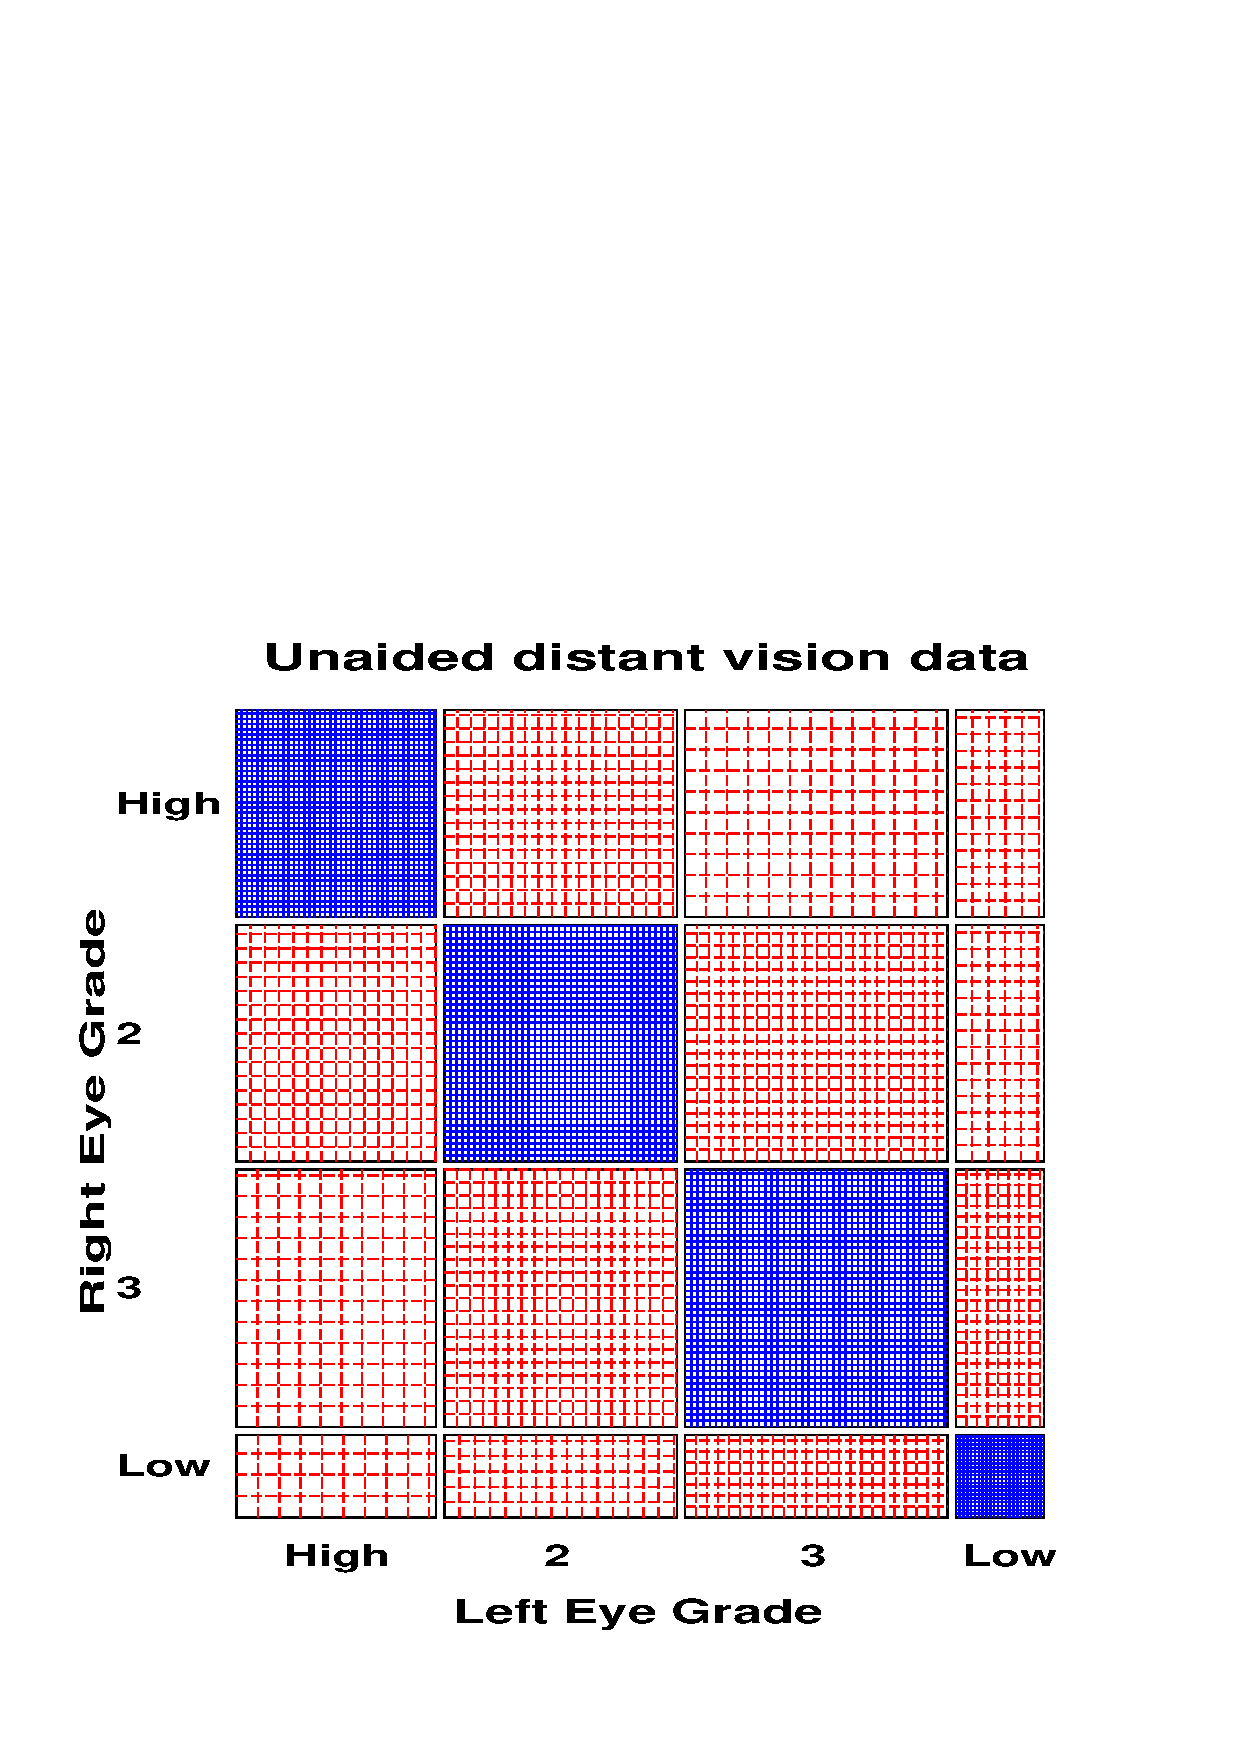
\includegraphics[width=1\linewidth,clip]{fig/sieve2}
  \end{minipage}%
 \hfill
 \begin{minipage}[c]{.33\textwidth}
  \includegraphics[width=1\linewidth,clip]{fig/mosaic3m1}
 \end{minipage}
  \rule{0.5pt}{4pt}\hrulefill\rule{0.5pt}{4pt} \\
	}
\date[VCD, 2012] % (optional)
{Short Course, 2012 \\
\small Web notes: \texttt{datavis.ca/courses/VCD/}}
% \\ SCS Short Course}

\subject{VCD}

% Delete this, if you do not want the table of contents to pop up at
% the beginning of each subsection:

\AtBeginSection[]
{
  \begin{frame}<beamer>
    \frametitle{Lecture outline}
    \tableofcontents[currentsection,currentsubsection,hideothersubsections]
  \end{frame}
}

%\includeonlylecture{Overview}
%\includeonlylecture{Two-way}
%\includeonlylecture{n-way}
%\includeonlylecture{Model}
\includeonlylecture{Polytomous}

\begin{document}

\begin{frame}[plain]
  \titlepage
\end{frame}

\lecture{Overview}{Overview}
\renewcommand{\FileName}{part1}
\part{Introduction}
\subsection{Goals and design principles for visual data display}\label{sec:intro-goals}

Designing good graphics is surely an art, but as surely, it is
one that ought to be informed by science.
In constructing a graph, quantitative and qualitative information is
encoded by visual features, such as position, size, texture, symbols
and color. This translation is reversed when a person studies a
graph. The representation of numerical magnitude and categorical
grouping, and the aperception of patterns and their \emph{meaning} must be extracted from the visual display.  

There are many views of graphs, of graphical perception, and of
the roles of data visualization in discovering and communicating
information.
On the one hand, one may regard a graphical display as a ``stimulus'' --
a package of information to be conveyed to an idealized observer.
From this perspective certain questions are of interest:  which
form or graphic aspect promotes greater accuracy or speed of judgment
(for a particular task or question)?  What aspects lead to greatest
memorability or impact? 
Cleveland \citep{ClevelandMcGill:84b,ClevelandMcGill:85,Cleveland:93:JCGS},
Lewandowsky and
Spence
\citep{LewandowskySpence:89,Spence:90} have made important contributions to our understanding of
these aspects of graphical display.

An alternative view regards a graphical display as an act
of communication---like a narrative, or even a poetic text or work of art. 
This perspective places the greatest emphasis on the desired
communication goal, and judges the effectiveness of a graphical
display in how well that goal is achieved.
\citet{Kosslyn:85,Kosslyn:89} and \citet{Tufte:83,Tufte:90,Tufte:97}
have articulated this perspective most clearly.

In this view,
an effective graphical display, like good writing, requires an
understanding of its purpose---what aspects of the data are to be
communicated to the viewer.  In writing we communicate most
effectively when we know our audience and tailor the message
appropriately. So too, we may construct a graph in different ways to
use ourselves, to present at a conference or meeting of our
colleagues, or to publish in a research report, or a communication
to a general audience
\cite[Ch. 1]{Friendly:91}.

\figref{fig:datadisp}
shows one organization of visualization methods in terms
of the primary use or intended communication goal,
the functional presentation goal, and suggested corresponding
design principles.
\begin{figure}[htbp]
  \centering 
  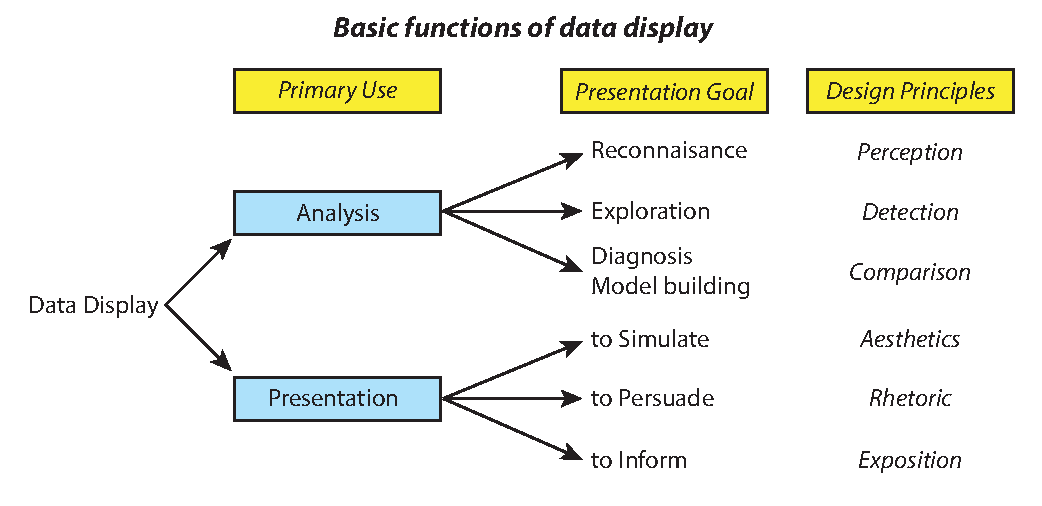
\includegraphics[scale=.8]{ch1/fig/datadisp}
  \caption[Basic functions of data display]{A taxonomy of the basic functions of data display by intended use and presentation goal}\label{fig:datadisp}
\end{figure}

The first distinction identifies \boldital{Analysis} or 
\boldital{Presentation} as the primary
communication goal of a data graphic
(with the understanding that a given graph may serve both purposes---or,
sadly, neither).

\subsubsection{Analysis graphs}
Graphs used for data analysis should clearly show the data, but they
should also ``force us to notice what we never
expected to see''
\cite[p. vi]{Tukey:77}.

Among graphical methods designed to help study or understand
a body of data, we may distinguish those designed for different
purposes.  As suggested in \figref{fig:datadisp}, each presentation goal
is associated with somewhat different design principles.
\begin{itemize}
\item \boldital{reconnaissance}---a preliminary examination, or an overview of a possibly complex terrain.
For this goal, we may be willing to sacrifice detail for a wider field of
view.
With a large, multi-way contingency table, for example, we might wish to
examine the collection of one-way and two-way marginal subtables
visually.  
\item \boldital{exploration}---graphs designed to help detect patterns or unusual
circumstances, or to suggest hypotheses, analyses or models.
For a binary response and a number of categorical or quantitative predictors,
a collection of smoothed plots of the response against each predictor
may suggest important variables to be included in a model,
extreme observations which should be examined, etc.
\item \boldital{diagnosis}---graphs designed to summarize or critique
a numerical statistical summary.
\end{itemize}

\subsubsection{Presentation graphs}
Presentation graphics have different goals as well.
We may wish to stimulate, or to persuade, or simply to inform.
As in writing, it is usually a good idea to know what it is you
want to say with a graph, and tailor its message to that goal.

It is often the case that a graph originally prepared as an aid
to data analysis can be transformed to one intended for presentation
by simple re-design.
Sometimes this entails removing detail useful for the analyst
but which may be detract from the major message;
sometimes this may involve adding titles or annotation to make the
message more immediately apparent.
In still other cases, we may decide to change the graphic format
to make visual comparisons easier for the intended audience.

For example, \figref{fig:glogist00} shows two views of the results
of fitting a logistic regression model to the arthritis treatment
data (described in \secref{sec:logist-qual}).
The left panel shows the observed (points) and predicted probabilities of
improvement ($\pm 1$ standard error, giving approximate 67\%
confidence intervals) in the form of a line graph.
The right panel shows a possible re-design of this graph for presentation
purposes.
%% two subfig side-by-side
\begin{figure}[htb]
 \begin{minipage}[c]{.49\linewidth}
  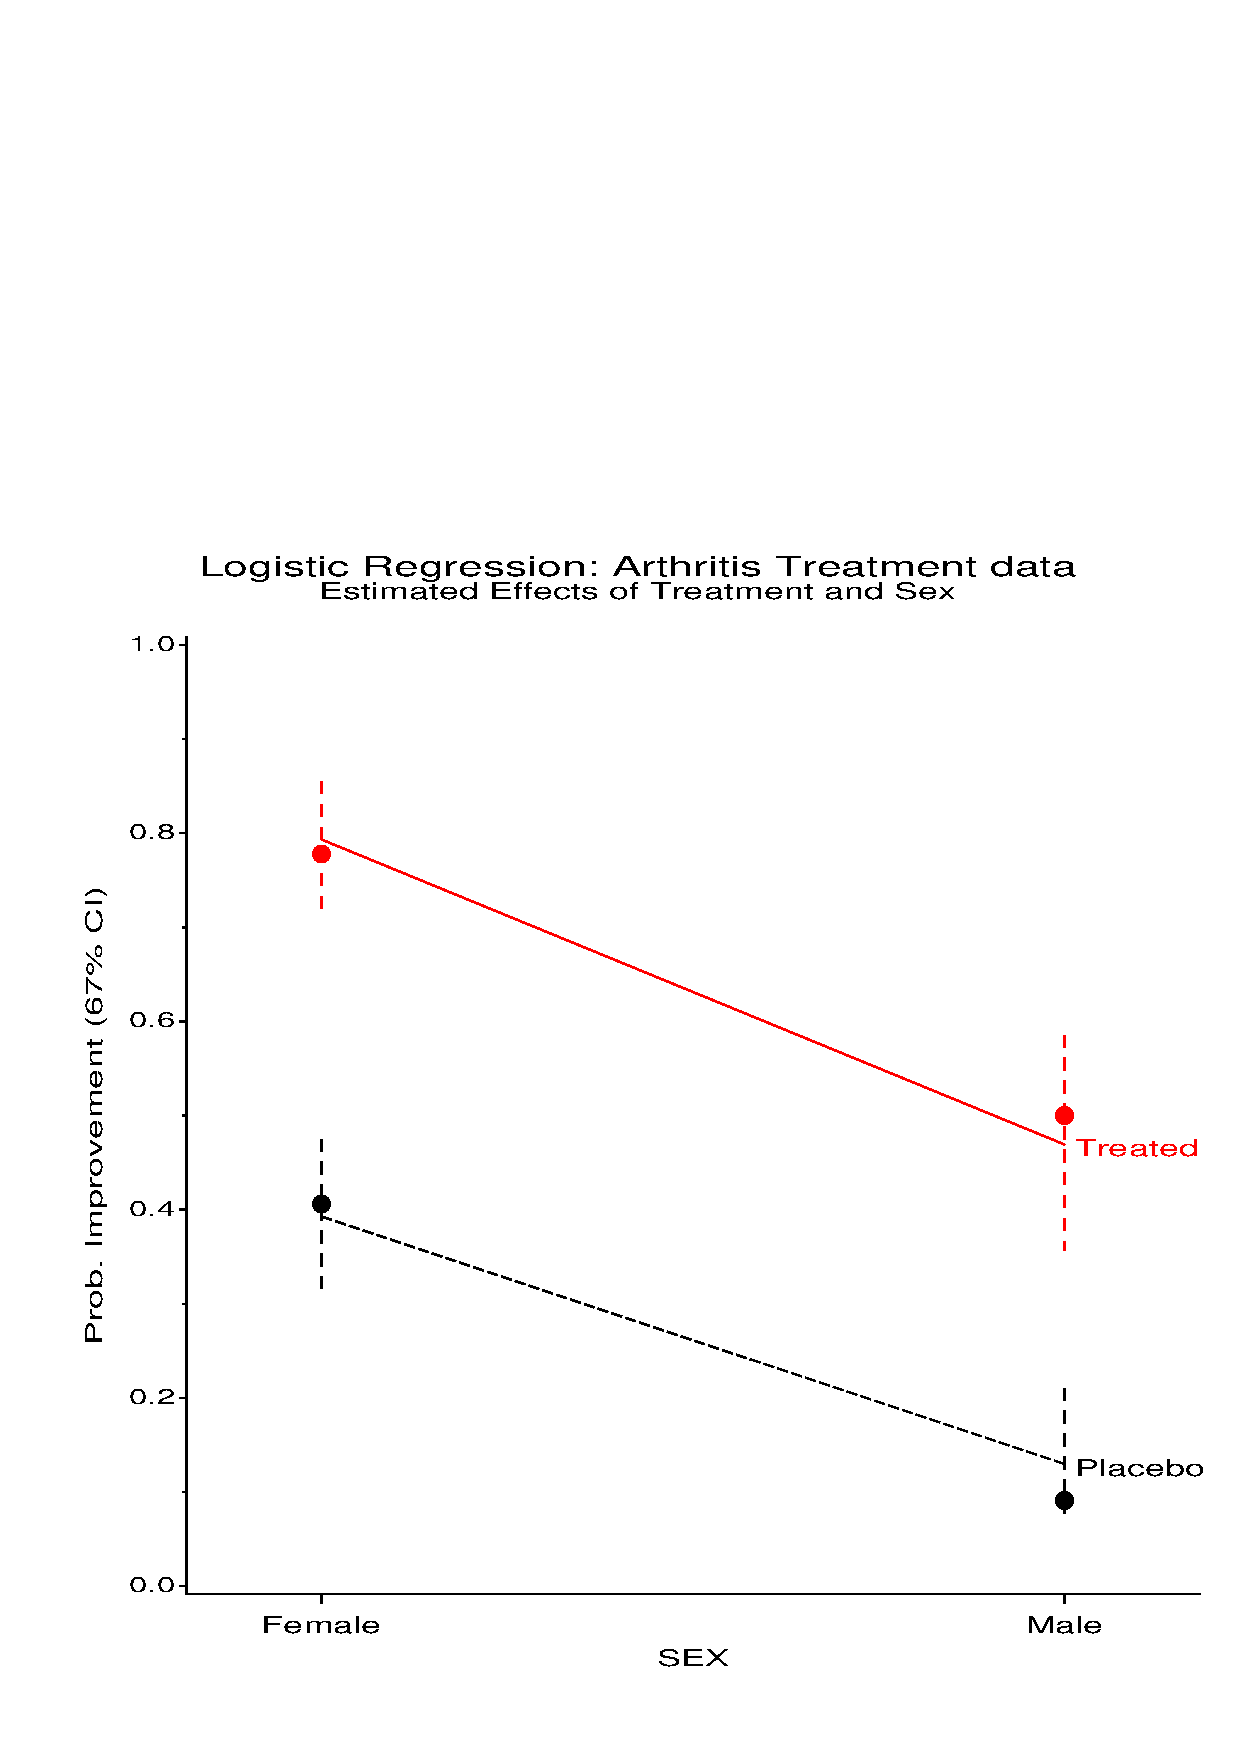
\includegraphics[width=1\linewidth]{ch6/fig/glogist11}
 \end{minipage}%
 \hfill
 \begin{minipage}[c]{.49\linewidth}
  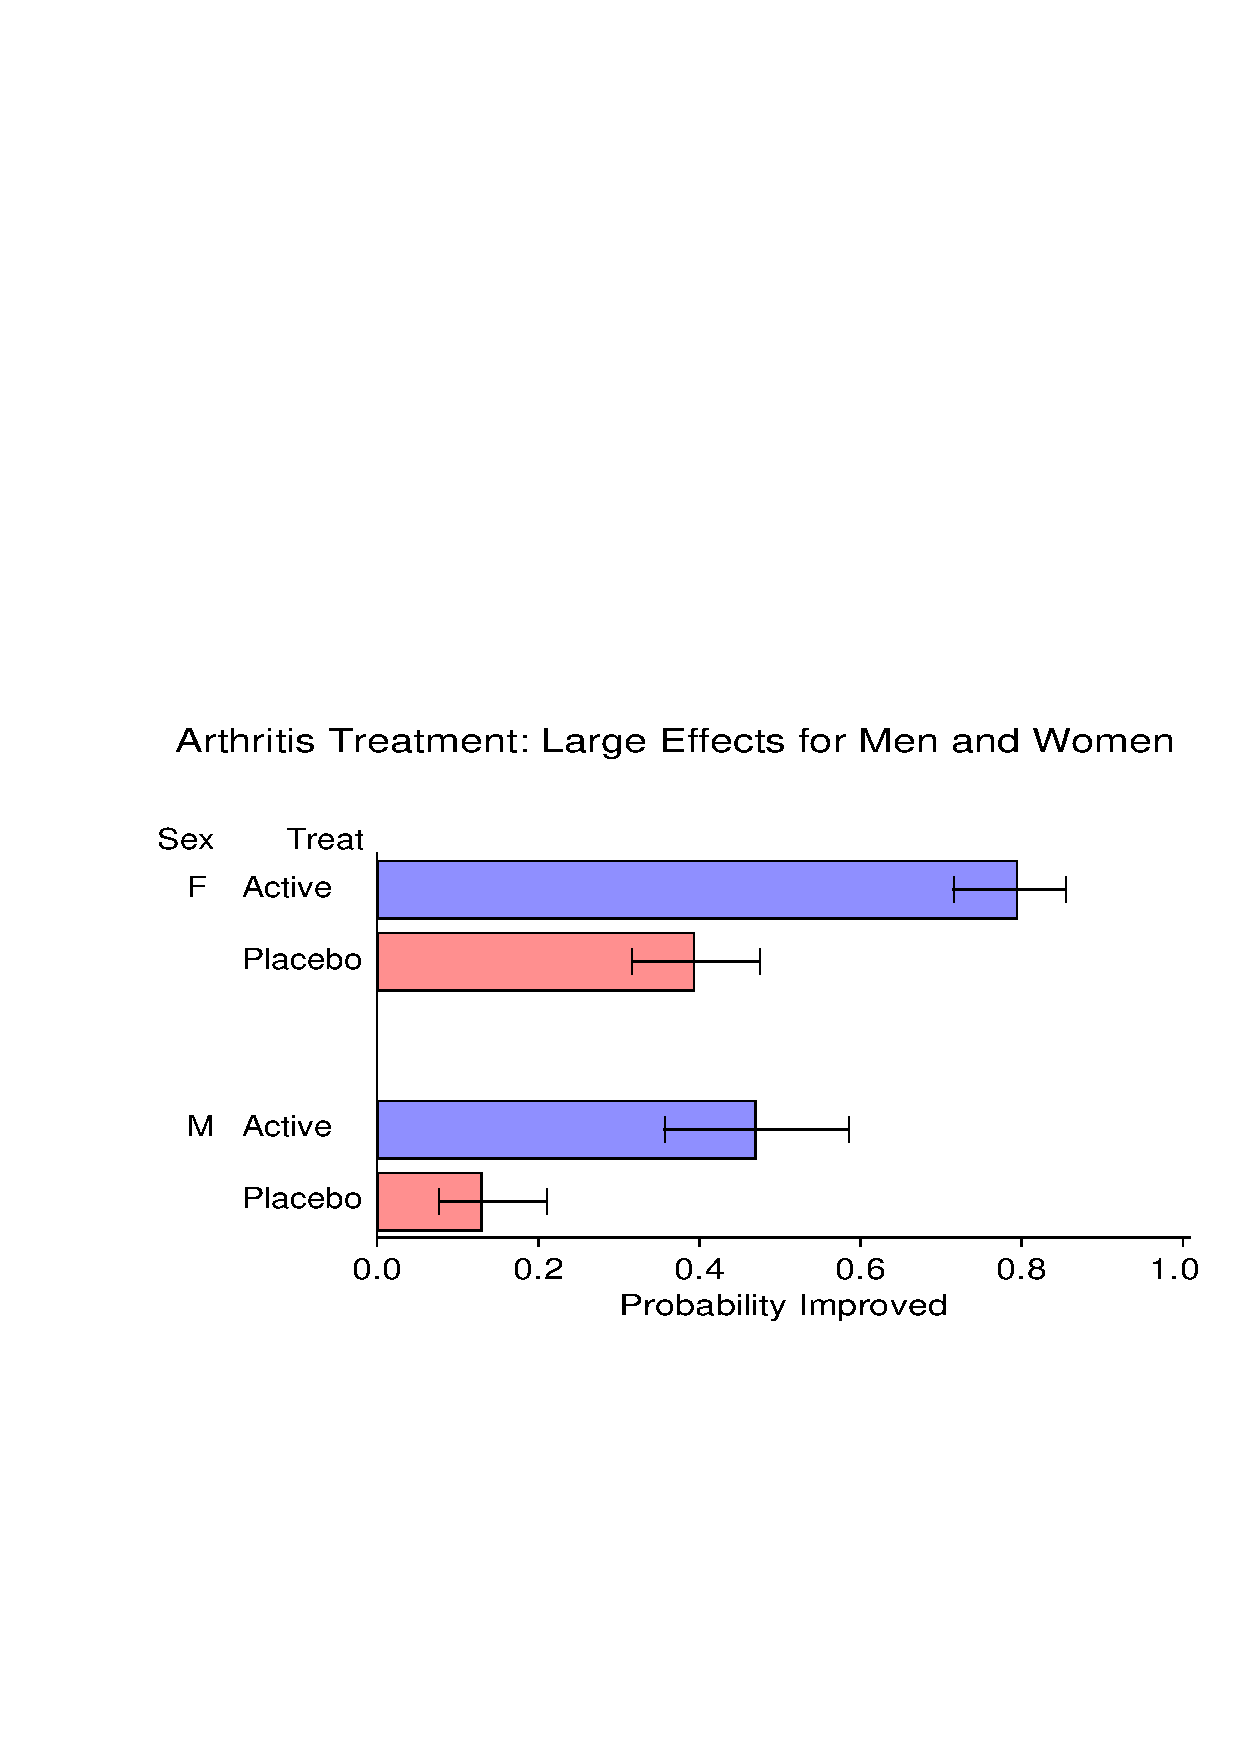
\includegraphics[width=1\linewidth,clip]{ch1/fig/glogist00}
 \end{minipage}
 \caption[Two graphical displays for arthritis treatment data]{Two graphical displays for arthritis treatment data. Left: initial analysis graph; right: re-design for presentation.}\label{fig:glogist00}
\end{figure}

The line graph might be preferred for analysis purposes, because it
shows
\begin{seriate}
\item the observed and fitted probabilities are quite similar,
\item there is a large effect of both treatment and sex, and
\item the effect of treatment is about the same for both men and women.
\end{seriate}
The presentation version contains the same predicted probabilities and error
bars as the original graph, but omits the observed probabilities
for simplicity.
The title explicitly
announces the conclusion to be drawn from the graph.



\section{Showing the structure of \loglin{} models}\label{sec:mosaic-struc}
The mosaic display can also be used to illuminate the relations among
variables in a \ctab{} which are represented in various \loglin{} models,
a point described by \citet{TheusLauer:99}.
Each of the model types depicted in \tabref{tab:hyp3way} has, in fact,
a characteristic shape and structure in a mosaic display. This,
in turn, leads to a clearer understanding of the structure which appears
in real data when a given model fits, the relations among the models,
and the use of mosaic displays.

%%
%% Table struc written by md2tex 29MAY98 08:46
%%
\begin{table}[htb]
 \caption{A $2 \times 2 \times 2$ table (artificial data)}
 \label{tab:struc}
 \begin{center}
  \begin{tabular}{|l|rrrr|r|}
   \hline
% & \multicolumn{4}{c|}{\bfseries\large B} & \rule{0in}{2.5ex}\\
 & \multicolumn{2}{c|}{B1} & \multicolumn{2}{c|}{B2} &  \\\cline{2-5}
% & \multicolumn{4}{c|}{\bfseries\large A} & \rule{0in}{2.5ex}\\
{\bfseries\large C} & A1 & A2 & A1 & A2& {\bfseries\large Total} \\
   \hline
C1   &     6 &    10 &   312 &    44 &   372 \\
C2   &    37 &    31 &   192 &    76 &   336 \\
   \hline
\rule{0in}{2.5ex}{\bfseries\large Total} &   43 &    41 &   504 &   120 &   708 \\
   \hline
  \end{tabular}
 \end{center}
\end{table}

To show this, we use artificial data for a $2 \times 2 \times 2$ table
shown in \tabref{tab:struc}.
We can force such a table to conform to any \loglin{} model
(e.g., $H_1$ -- $H_4$)
simply by finding the expected frequencies under that model
and constructing a mosaic depicting the expected frequencies.

\subsection{Mutual independence}
For example, to show the structure of a table which fits
mutual independence, $H_1$, use the \FUNC{IPF} to find the
fitted values, \texttt{fit}, as

\begin{verbatim}
proc iml;
   table = { ... };
   dim= {2 2 2};
   vnames={A B C};
   lnames = {'A1' 'A2',  'B1' 'B2',  'C1' 'C2'};

   config = {1 2 3};
   call ipf(fit,status,dim,table,config);
   fittype='MUTUAL';
   print fittype config[f=4.] fit[f=7.2];
\end{verbatim}
The fitted frequencies then have the same one-way margins as the
data in \tabref{tab:struc}, but have no two-way or higher associations.
We then display a mosaic for the \emph{fitted frequencies}
to see what mutual independence looks like in a three-way table.
\begin{output}
   FITTYPE  CONFIG             FIT
   MUTUAL      1   2   3     34.10   10.04  253.31   74.56
                             30.80    9.07  228.79   67.34
\end{output}
What you see in a mosaic display depends, in large measure, on the order in
which the table variables are entered.
For three variables there are $3!=6$ possible orders;  conveniently,
they are all shown in the mosaic matrix.
In this display we show the three-way mosaic (\texttt{plots=3;})
for each pair of variables, using the fitted values as the ``data.''
The statements below produce \figref{fig:mosfit-1}.
\begin{figure}[htb]
  \centering
  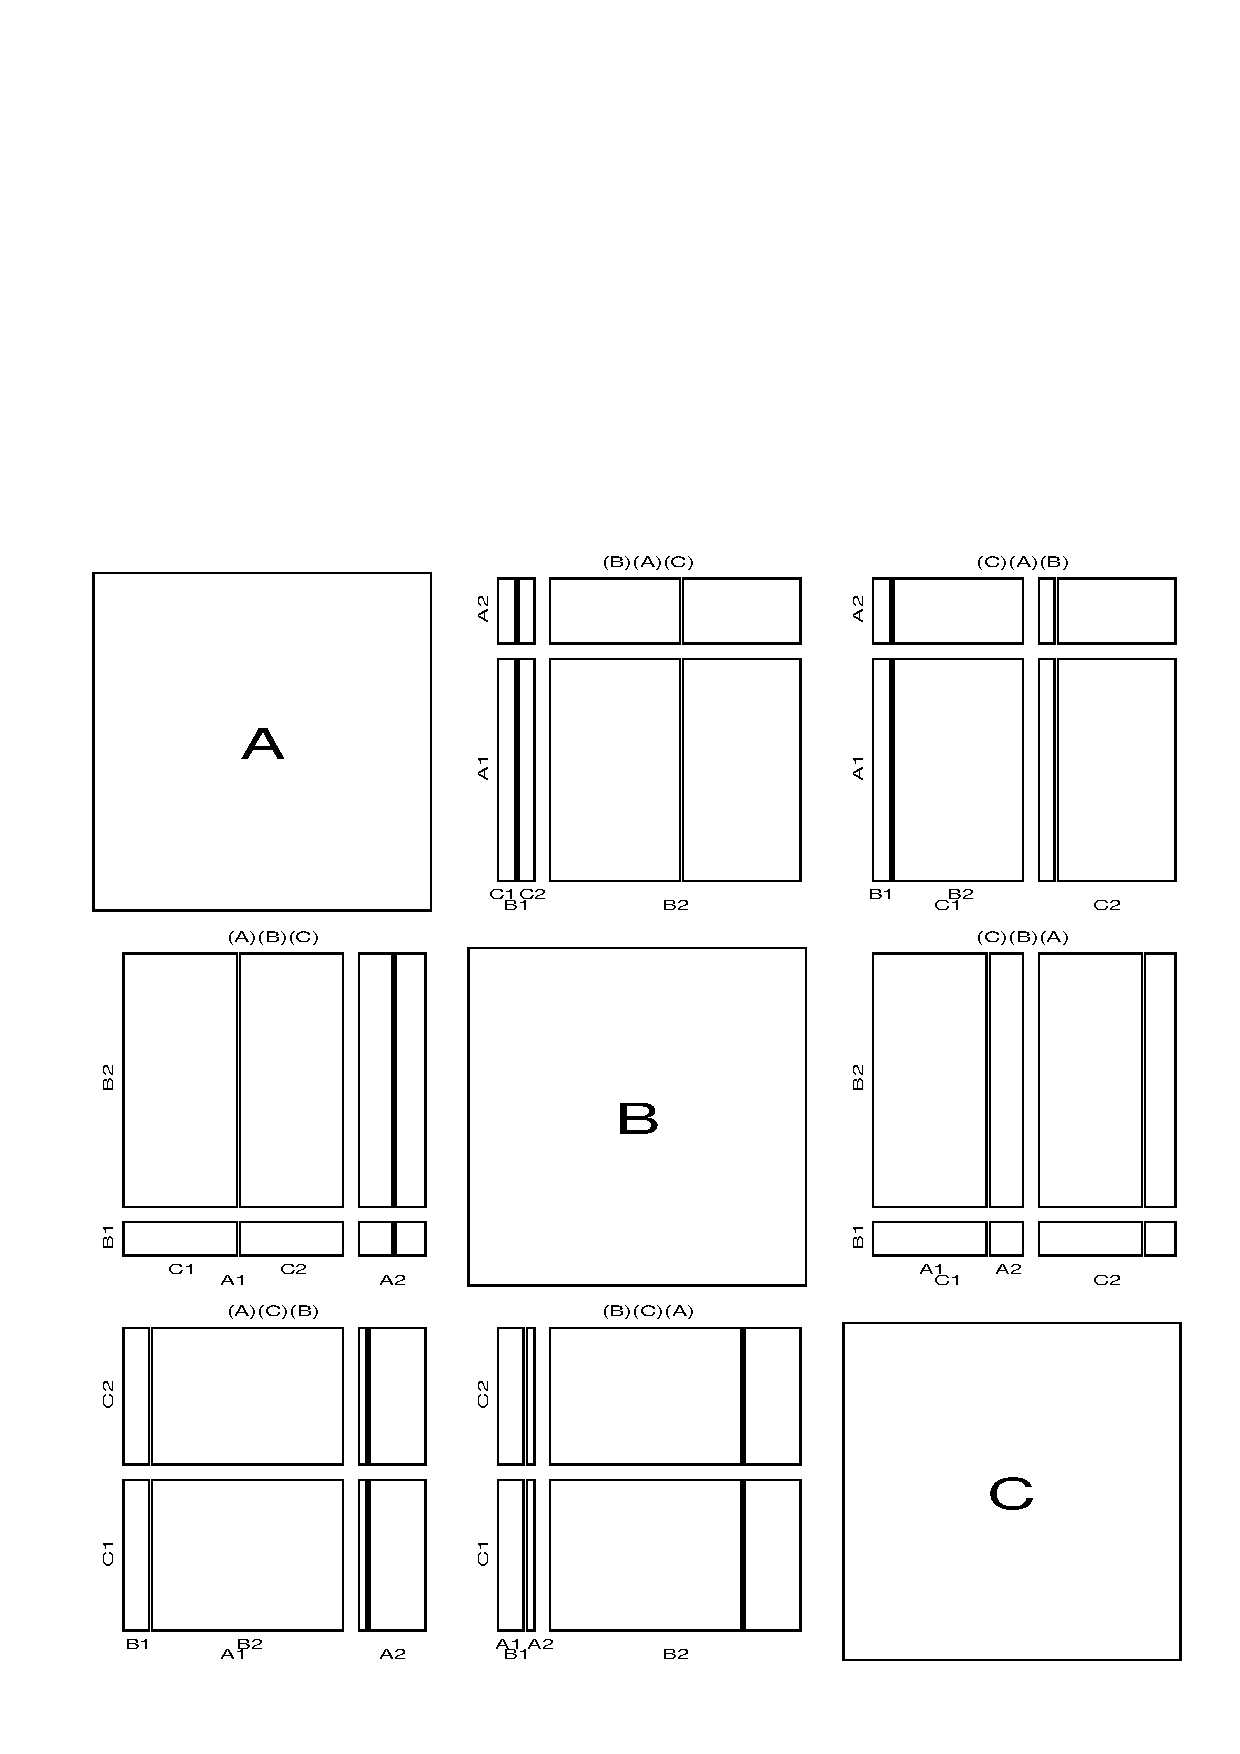
\includegraphics[scale=.6]{ch4/fig/mosfit-1}
  \caption[Mosaic matrix for mutual independence]{Mosaic matrix for mutual independence.  All panels show marginal and conditional independence among all three pairs of variables.}%
  \label{fig:mosfit-1}
\end{figure}

\begin{verbatim}
   plots=3;
   title=fittype+'&MODEL';
   space={12 5};
   run mosmat(dim, fit, vnames, lnames, plots, title);
quit;
%panels(rows=3, cols=3, equate=Y, order=down);
\end{verbatim}


In this figure the same data are shown in all the off-diagonal panels
and the mutual independence model was fitted in each case, but with the
table variables permuted.  All residuals are exactly zero in all cells,
by construction.
We see that in each view, the four large
tiles, corresponding to the first two variables align, indicating
that these two variable are marginally independent.
For example, in the $(1,2)$ panel, $A$ and $B$ are independent, collapsed
over variable $C$.

Moreover, comparing the top half to the bottom half
in any panel we see that the divisions by the third variable
are the same for both levels of the second variable.
In the $(1, 2)$ panel, for example, $A$ and $C$ are independent at
$B1$, and also independent at  $B2$.
This means, though, that $A$ and $B$ are conditionally independent
given $C$ ($A \perp B \given C$).
Because this holds in all six panels, we see that mutual independence
is equivalent to \emph{all pairs} of variables being conditionally
independent, given the remaining one,  ($X \perp Y \given Z$) for all
permutations of variables.

\subsection{Joint independence}
The model of joint independence, $H_2: \: (A, B) \perp C$, or
equivalently, the \loglin{} model $[A B][C]$
may be visualized similarly by the mosaic matrix in \figref{fig:mosfit-21},
in which the data were replaced by fitted values under this model.
\begin{figure}[htb]
  \centering
  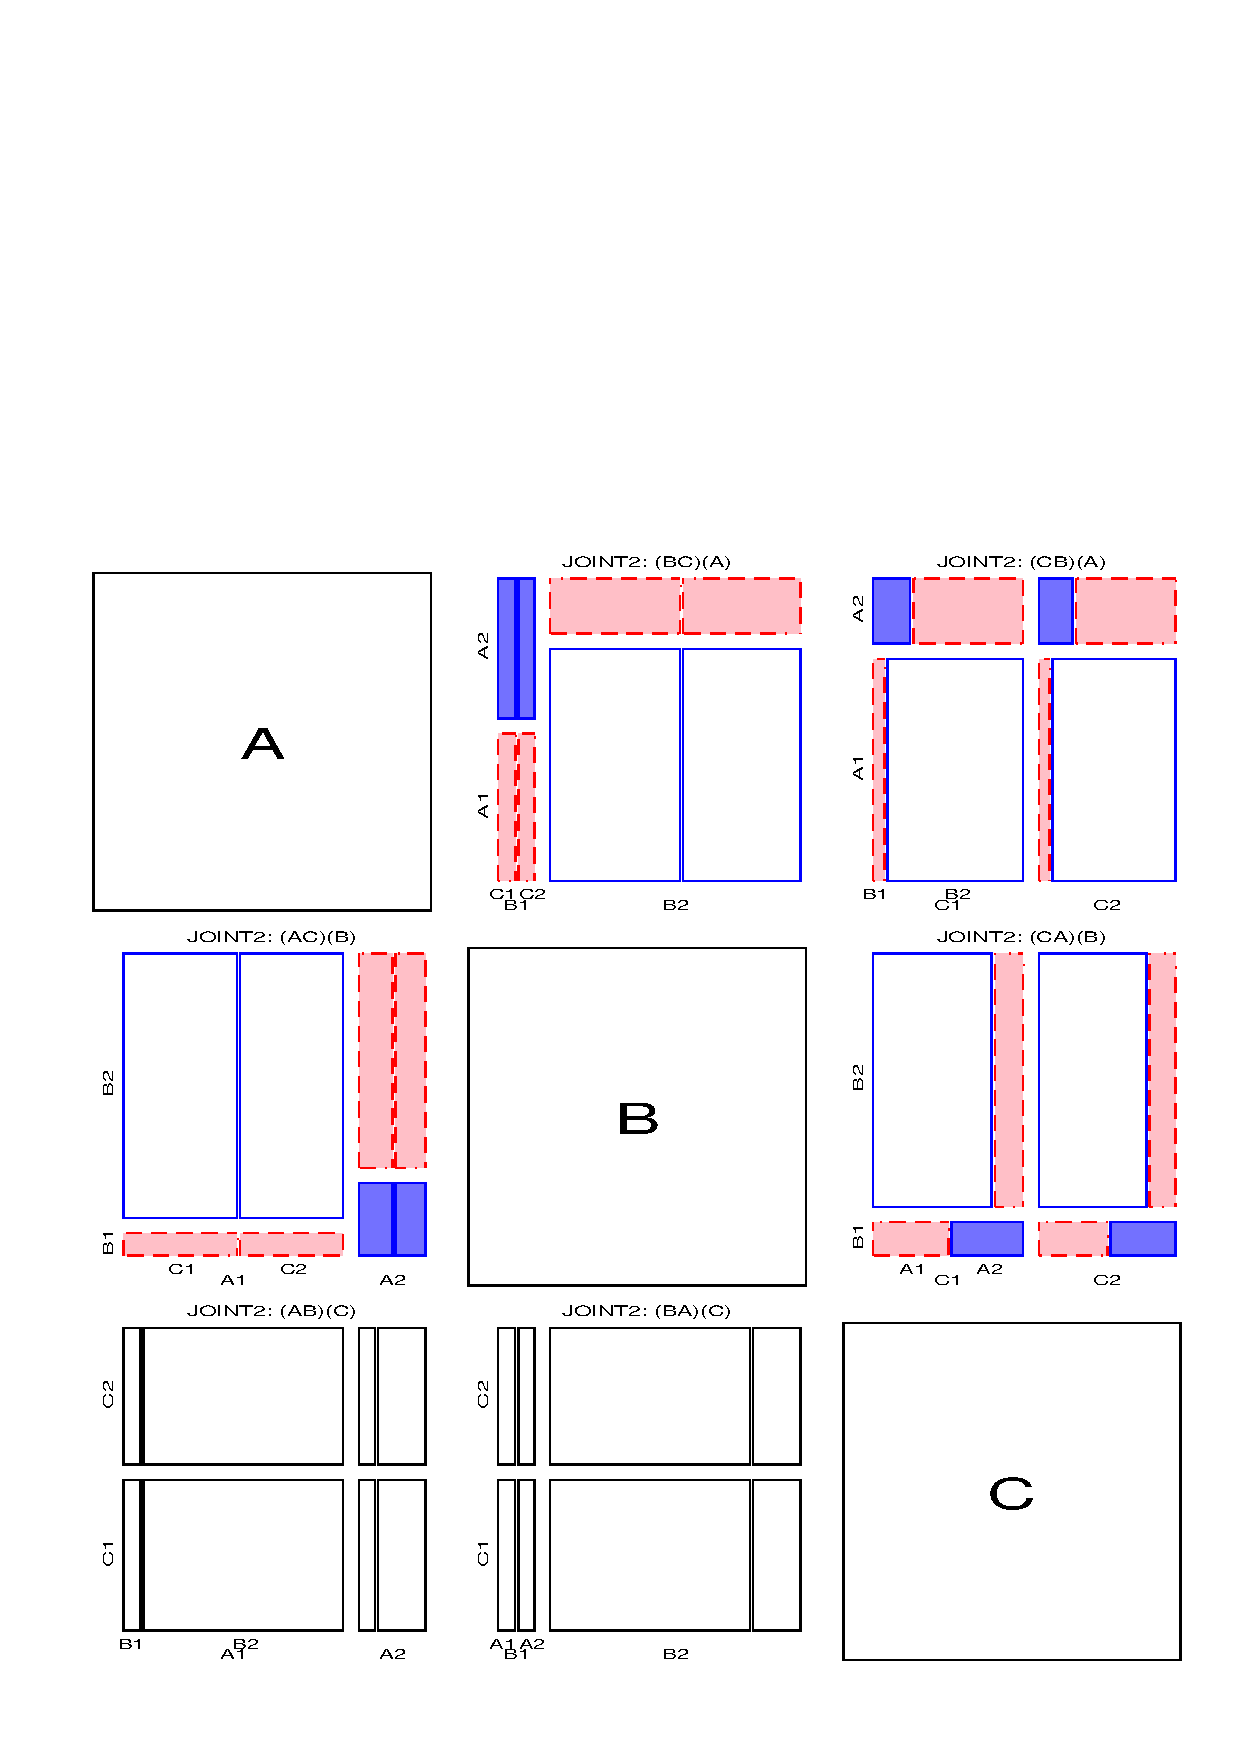
\includegraphics[scale=.6]{ch4/fig/mosfit-21}
  \caption[Mosaic matrix for joint independence]{Mosaic matrix for joint independence.  The bottom row shows that $A$ and $B$ are each independent
 of $C$, and  also
conditionally independent of $C$}%
  \label{fig:mosfit-21}
\end{figure}
\begin{verbatim}
   ...
   config = t({1 2, 3 0});
   call ipf(fit,status,dim,table,config);
   fittype='JOINT2';
   ...
\end{verbatim}
which gives these fitted frequencies.
\begin{output}
   FITTYPE  CONFIG        FIT
   JOINT2      1   3    22.59   21.54  264.81   63.05
               2   0    20.41   19.46  239.19   56.95
\end{output}
The \texttt{fittype='JOINT2';} specifies that in each panel the fitted model
is that wherein the first and third variable are independent of the second.
Now, in \figref{fig:mosfit-21}, the same model is fit in both panels in
each row,  but the second, distinguished variable differs from
row to row.

We see in row 3, where $C$ is the second variable, that $C$ is independent
of $A$, and also independent of $B$, and these models have residuals
equal to zero.
The models fit in the other four panels have non-zero residuals.
However, the $(1, 2)$ and $(2, 1)$ panels show that
$B \perp C \given A$, and $A \perp C \given B$, respectively, because
the top and bottom portions are both divided equally by the third table
variable.
This relation does not hold, however, in the $(1, 3)$ and $(2, 3)$ panels.
Thus, joint independence implies that conditional independence hold
as well, but only for the two variables which enter jointly.

The appearance in the bottom row of \figref{fig:mosfit-21}
that $A$ and $B$ are marginally independent, is
misleading, because the $AB$ association is fit exactly in these models.
To see the marginal relations under $[A B][C]$ explicitly,
we can just change the \texttt{plots} value to \texttt{plots=2;},
so that the model of (marginal) independence is fit to the first two
variables in each panel and only these variables are displayed.
This plot appears in \figref{fig:mosfit-22}, and shows
clearly that $A$ and $B$ are each marginally independent of $C$,
but not of each other.
\begin{figure}[htb]
  \centering
  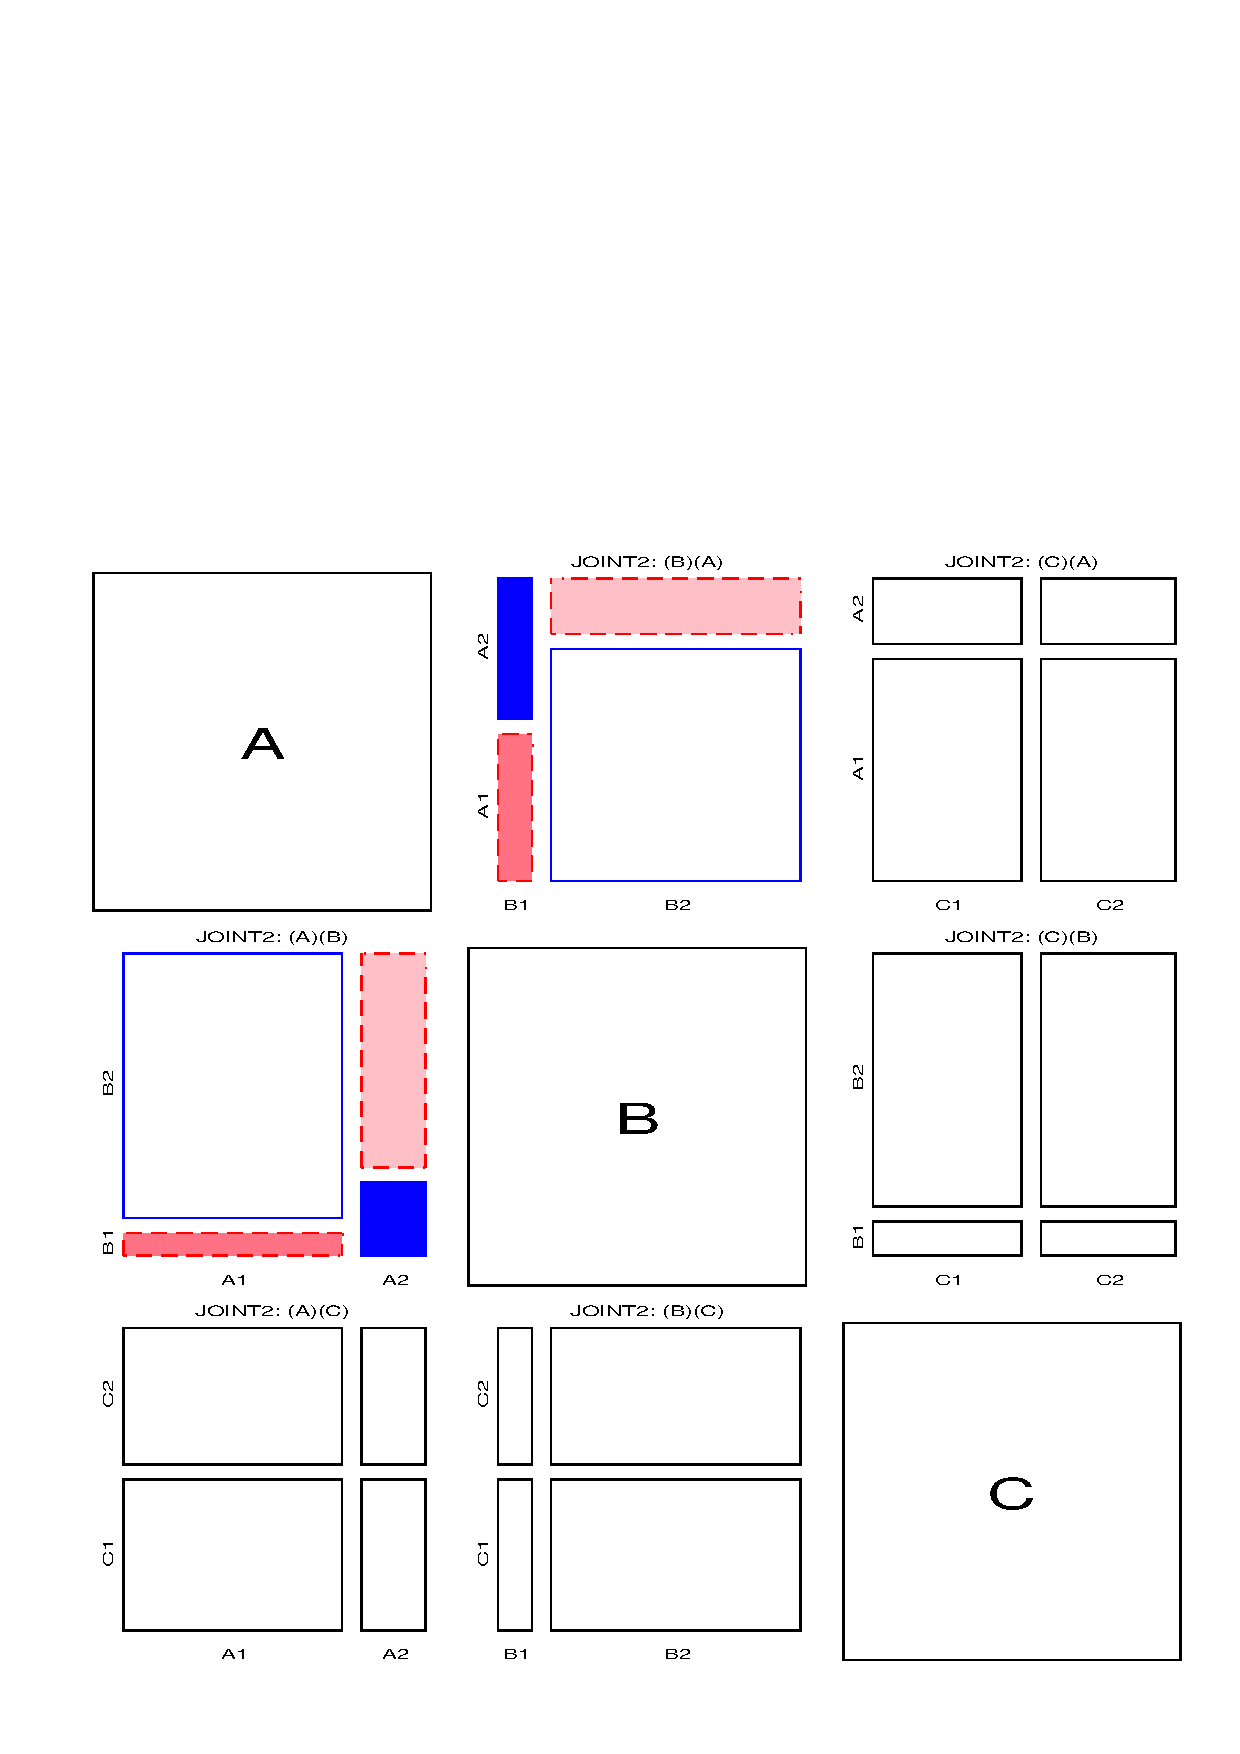
\includegraphics[scale=.6]{ch4/fig/mosfit-22}
  \caption[Marginal relations under joint independence]{Marginal relations under joint independence.  $A$ and $B$ are each marginally independent
 of $C$}%
  \label{fig:mosfit-22}
\end{figure}

\subsection{Conditional independence}
For conditional independence, $H_3: \: A  \perp B \given C$,
or $[A C][B C]$, we proceed similarly,  using
\begin{verbatim}
   config = t({1 2, 2 3});
   call ipf(fit,status,dim,table,config);
   fittype='CONDIT1';
   ...
\end{verbatim}
to obtain frequencies which fit this model exactly.
The resulting three-way mosaic matrix is shown in \figref{fig:mosfit-3}.
\begin{figure}[htb]
  \centering
  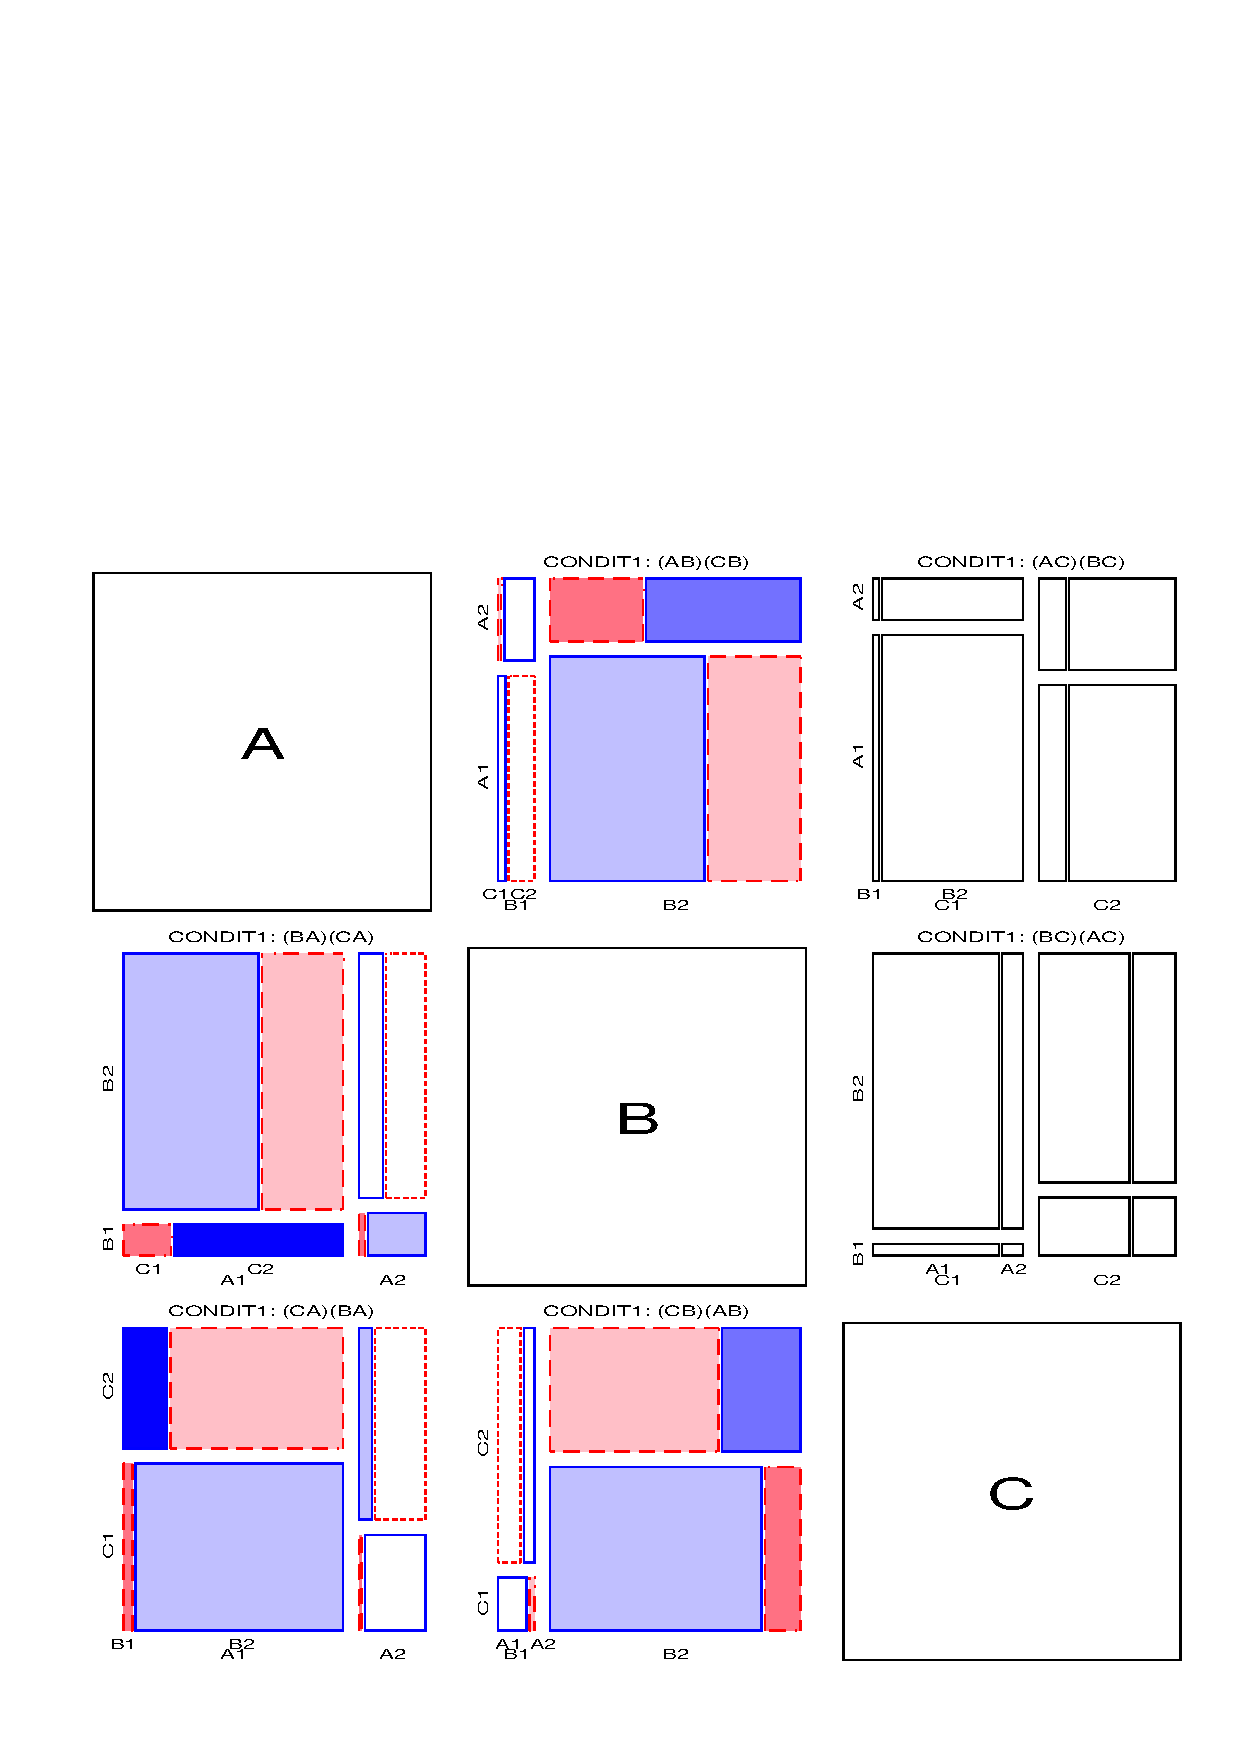
\includegraphics[scale=.6]{ch4/fig/mosfit-3}
  \caption[Mosaic matrix for conditional independence]{Mosaic matrix for conditional independence}%
  \label{fig:mosfit-3}
\end{figure}
We now see the characteristic signature of conditional independence in the
$(1, 3)$ and $(2, 3)$ panels, where $A$ and $B$ are independent at
each level of $C$. But no independence relations appear in the four
large blocks of the first two variables in any panel, so
no pair of variables is marginally independent.%
\footnote{In this data $A$ and $B$ have quite a weak association, as
may be seen in the $(1, 2)$ and $(2, 1)$ panels, where the large blocks
nearly align.}

\section{Overview}

\subsection{What is categorical data?}
\renewcommand{\FileName}{whatis}

% slide template
\begin{frame}
  \frametitle{What is categorical data?}
  \begin{itemize}
	\item Simplest case: 1-way frequency distribution
      \begin{itemize*}
	  \item Unordered factor
	  \begin{flushright}
	  \includegraphics[width=.9\dispwidth]{fig/whatis1}
	  \end{flushright}
	  \item Ordered, quantitative factor
	  \begin{flushright}
	  \includegraphics[width=.9\dispwidth]{fig/whatis2}
	  \end{flushright}
	  \end{itemize*}
  \end{itemize}
\end{frame}

\begin{frame}
  \frametitle{What is categorical data?}
  \begin{itemize}
	\item Contingency tables ($2 \times 2 \times \dots$)
      \begin{itemize*}
	  \item Two-way
	  \begin{flushright}
	  \includegraphics[width=.8\dispwidth]{fig/whatis3}
	  \end{flushright}
	  \item Three-way
	  \begin{flushright}
	  \includegraphics[width=.9\dispwidth]{fig/whatis4}
	  \end{flushright}
	  \end{itemize*}
  \end{itemize}
\end{frame}

\begin{frame}
  \frametitle{What is categorical data?}
  \begin{itemize}
	\item Contingency tables (larger)
      \begin{itemize*}
	  \item Two-way
	  \begin{flushright}
	  \includegraphics[width=.7\dispwidth]{fig/whatis5}
	  \end{flushright}
	  \item Three-way
	  \begin{flushright}
	  \includegraphics[width=.8\dispwidth]{fig/whatis6}
	  \end{flushright}
	  \end{itemize*}
  \end{itemize}
\end{frame}


% two columns with text and figure
\begin{frame}
  \frametitle{Table and case-form}
  \begin{columns}[T]
    \begin{column}{.6\textwidth}
	  \begin{itemize}
		\item<1> The previous examples were shown in \alert{table} form
		  \begin{itemize*}
		    \item \# observations = \# cells in the table
			\item variables: factors + COUNT
		  \end{itemize*}
		\item<2> Each has an equivalent representation in \alert{case} form
		  \begin{itemize*}
		    \item \# observations = total COUNT
			\item variables: factors 
		  \end{itemize*}
		\item<3> Case form is required if there are continuous variables
	  \end{itemize}
    \end{column}
    \begin{column}{.4\textwidth}
    \includegraphics<1>[width=\textwidth,clip]{fig/whatis6}
    \includegraphics<2>[width=\textwidth,clip]{fig/whatis7}
    \includegraphics<3>[width=\textwidth,clip]{fig/whatis8}
    \end{column}
  \end{columns}
\end{frame}


\subsection{Methods}
%\section*{Overview and organization of this book}

This book is divided into three parts. Part I, Chapters 1--3, contains 
introductory material on graphical methods for discrete data, 
basic \R skills needed for the book, and methods for fitting
and visualizing one-way discrete distributions.

Part II, Chapters 4--6, is concerned largely with 
simple, traditional non-parametric tests and exploratory methods for
visualizing patterns of association in two-way and larger frequency tables.
Some of the discussion here introduces ideas and notation for \loglin
models that are treated more generally in Part III.

Part III, Chapters 7--11, discusses model-based methods for the
analysis of discrete data.  These are all examples of generalized
linear models.  However, for our purposes, it has proved more convenient
to develop this topic from the specific cases (logistic regression, \loglin models)
to the general rather than the reverse.

\begin{description}
\item[\chref{ch:intro}: \emph{Introduction}.]
Categorical data require different statistical and graphical methods
than commonly used for quantitative data.
This chapter outlines the basic orientation
of the book toward visualization methods and some key distinctions regarding the
analysis and visualization of categorical data.

\item[\chref{ch:working}: \emph{Working with Categorical Data}.]
Categorical data can be represented in various forms:
case form, frequency form, and table form.  This chapter
describes and illustrates the skills and techniques in \R
needed to input, create, and manipulate \R data objects
to represent categorical data, and convert these from one
form to another for the purposes of statistical analysis
and visualization, which are the subject of the remainder of the book.

\item[\chref{ch:discrete}: \emph{Fitting and Graphing Discrete Distributions}.]
Understanding and visualizing discrete data distributions provides a
building block for model-based methods discussed in Part III.
This chapter introduces the well-known discrete distributions---
the binomial, Poisson, negative-binomial, and others---
in the simplest case of a one-way frequency table.

\item[\chref{ch:twoway}: \emph{Two-Way Contingency Tables}.]
The analysis of two-way frequency tables concerns the association
between two variables.  A variety of specialized graphical
displays help to visualize the pattern of association,
using area of some region to represent the frequency in a cell.
Some of these methods are focused
on visualizing an odds ratio (for $2 \times 2$ tables), or the general
pattern of association, or the agreement between row and column
categories in square tables.

\item[\chref{ch:mosaic}: \emph{Mosaic Displays for $n$-Way Tables}.]
This chapter introduces mosaic displays, designed to
help to visualize the pattern of associations
among variables in two-way and larger tables.  
Extensions of
this technique can reveal partial associations and marginal associations,
and shed light on the structure of \loglin\ models themselves.

\item[\chref{ch:corresp}: \emph{Correspondence Analysis}.]
Correspondence analysis provides visualizations of associations in a two-way \ctab
in a small number of dimensions.
Multiple correspondence analysis extends this technique to \nway
tables.  Other graphical methods, including mosaic matrices and biplots,
provide complementary views of \loglin models for two-way and \nway
\ctabs.

\item[\chref{ch:logistic}: \emph{Logistic Regression Models}.]
This chapter introduces the modeling framework for categorical data in the simple
situation where we have a categorical response variable, often binary, and one or
more explanatory variables. A fitted model provides both statistical
inference and prediction, accompanied by measures of uncertainty.
Data visualization methods for discrete response data must often rely
on smoothing techniques, including both direct, non-parametric smoothing
and the implicit smoothing that results from a fitted parametric model.
Diagnostic plots help us to detect influential observations that may distort
our results.

\item[\chref{ch:polytomous}: \emph{Models for Polytomous Responses}.]
This chapter generalizes logistic regression models for a binary response to
handle a multi-category (polytomous) response.  Different models are available depending on
whether the response categories are nominal or ordinal.
Visualization methods for such models are mostly straightforward extensions
of those used for binary responses presented in \chref{ch:logistic}.

\item[\chref{ch:loglin}: \emph{Loglinear and Logit Models for Contingency Tables}.]
This chapter extends the model-building approach to \loglin and logit
models. These comprise another special case of generalized linear models
designed for \ctabs of frequencies.  They
are most easily interpreted through
visualizations, including mosaic displays and effect plots of associated
logit models.  

\item[\chref{ch:loglin2}: \emph{Extending Loglinear Models}.]
Loglinear models have special forms to represent additional structure in the
variables in contingency tables.  Models for ordinal factors allow a more
parsimonious description of associations.  Models for square tables
allow a wide range of specific models for the relationship between
variables with the same categories.  Another extended class of
models arise when there are two or more response variables.


\item[\chref{ch:glm}: \emph{Generalized Linear Models}.]
Generalized linear models extend the familiar linear models of
regression and ANOVA to
include counted data, frequencies, and other data for which the
assumptions of independent, normal errors are not reasonable.
We rely on the analogies between ordinary and generalized linear
models (GLMs) to develop visualization methods to explore the data,
display the fitted relationships, and check model assumptions.
The main focus of this chapter is on models for count data.

\end{description}







\subsection{Software: SAS}
\renewcommand{\FileName}{vcdmacros}

\begin{frame}
\frametitle{\VCD\ Macros \& \IML\ programs}
\begin{itemize}
\item Macros, \Dset{}s available at \url{datavis.ca/vcd/}
\end{itemize}

\begin{block}{Discrete distributions}<1->
\begin{proglist*}
	\item[DISTPLOT] Plots for discrete distributions 
	\item[GOODFIT] Goodness-of-fit for discrete distributions 
	\item[ORDPLOT] Ord plot for discrete distributions 
	\item[POISPLOT] Poissonness plot 
	\item[ROOTGRAM] Hanging rootograms 
\end{proglist*}
\end{block}

\begin{block}{Two-way and $n$-way tables}<2->
\begin{proglist*}
	\item[AGREEPLOT] Observer agreement chart 
	\item[CORRESP] Plot \PROC{CORRESP} results 
	\item[FFOLD] Fourfold displays for $2 \times 2 \times k$ tables
%	\item[FOURFOLD] Fourfold displays for $2 \times 2 \times k$ tables (\IML)
	\item[SIEVEPLOT] Sieve diagrams
	\item[MOSAIC] Mosaic displays 
%	\item[MOSAICS] \IML{} modules for mosaic displays 
	\item[MOSMAT] Mosaic matrices 
	\item[TABLE] Construct a grouped frequency table, with recoding 
	\item[TRIPLOT] Trilinear plots for $n \times 3$ tables 
\end{proglist*}
\end{block}
\end{frame}

\begin{frame}
\begin{block}{Model-based methods}<1->
\begin{proglist*}
	\item[ADDVAR] Added variable plots for logistic regression 
	\item[CATPLOT] Plot results from \PROC{CATMOD}
	\item[HALFNORM] Half-normal plots for generalized linear models 
	\item[INFLGLIM] Influence plots for generalized linear models 
	\item[INFLOGIS] Influence plots for logistic regression 
	\item[LOGODDS] Plot empirical logits and probabilities for binary data 
	\item[POWERLOG] Power calculations for logistic regression 
%	\item[POWERRxC] Power calculations for two-way frequency table 
%	\item[POWER2x2] Power calculations for a $2\times 2$ table 
%	\item[ROBUST] Robust fitting for linear models 
%	\item[TWOWAY] Two-way table display 
\end{proglist*}
\end{block}

\begin{block}{Utility macros}<2->
\begin{proglist}
	\item[DUMMY] Create dummy variables 
	\item[LAGS] Calculate lagged frequencies for sequential analysis 
	\item[PANELS] Arrange multiple plots in a panelled display 
	\item[SORT] Sort a dataset by the value of a statistic or formatted value 
	\item[Utility] Graphics utility macros:
	\pname{bars},
	\pname{equate},
	\pname{gdispla},
	\pname{gensym},
	\pname{gskip},
	\pname{label},
	\pname{points},
	\pname{pscale}
\end{proglist}
\end{block}
\VCD\ Archive (\texttt{vcdprog.zip}) available at:
\url{http://datavis.ca/courses/VCD/vcdprog.zip}
\end{frame}


\subsection{Software: R}
\renewcommand{\FileName}{vcdpackage}

\begin{frame}
\frametitle{R software and the \texttt{vcd} package}
\begin{itemize}
\item R software and the \texttt{vcd} package, 
available at \url{www.r-project.org}
\end{itemize}

\begin{block}{Discrete distributions}<1->
\begin{proglist}
	\item[distplot] Plots for discrete distributions 
	\item[goodfit] Goodness-of-fit for discrete distributions 
	\item[ordplot] Ord plot for discrete distributions 
	\item[poisplot] Poissonness plot 
	\item[rootgram] Hanging rootograms 
\end{proglist}
\end{block}

\begin{block}{Two-way and $n$-way tables}<2->
\begin{proglist}
	\item[agreementplot] Observer agreement chart 
	\item[fourfold] Fourfold displays for $2 \times 2 \times k$ tables 
	\item[sieve] Sieve diagrams
	\item[mosaic] Mosaic displays 
	\item[pairs.table] Matrix of pairwise association displays 
	\item[structable] Manipulate high-dimensional contingency tables 
	\item[triplot] Trilinear plots for $n \times 3$ tables 
\end{proglist}
\end{block}
\end{frame}

\begin{frame}[t]
\frametitle{R software: Other packages}
\begin{block}{Model-based methods}
\begin{proglist}
	\item[glm] Fitting generalized linear models 
	\item[gnm] Fitting generalized \emph{non-linear} models, e.g., RC(1) model
	\item[loglm] MASS package: Fitting loglinear models 
	\item[Rcmdr] Menu-driven package for statistical analysis and graphics
	\item[car] Graphics and extensions of generalized linear models 
	\item[effects] Effects plots for generalized linear models 
\end{proglist}
\end{block}
%\begin{itemize}
%\item Additional material in the  \texttt{vcdExtra} package, 
%available at \url{http://R-Forge.R-Project.org/vcdextra}
%\end{itemize}
\begin{block}{vcdExtra package}
\begin{proglist}
    \item[vcd-tutorial] Vignette on working with categorical data and the vcd package
	\item[mosaic.glm] mosaic displays for GLMs and GNMs
	\item[mosaic3d] 3D mosaic displays 
	\item[glmlist] Methods for working with lists of models
\end{proglist}
\end{block}

\end{frame}


\section{Discrete distributions}
%\subsection{Using SAS}
\renewcommand{\FileName}{discrete}
\begin{comment}
\begin{frame}
  \frametitle{Discrete distributions}  
  \begin{itemize}
	\item {\large\bfseries Counts of occurrences:} accidents, words in text, 
	blood cells with some characteristic.
	\item{\large\bfseries Data:} Basic outcome value, \(k \,  , \,  k = 0 , 1, \dots\),
	and number of observations, \(n_k\), with that value.
	\item {\large\bfseries Example:} \emph{Federalist Papers}--- disputed authorship 
      \begin{itemize*}
	  \item 77 essays by Hamilton, Jay \& Madison: persuade NY voters to ratify Constitution, all
	  signed with pseudonym (``Publius'')
	  \item 65 known, 12 disputed (H \& M both claimed sole authorship)
	  \item \citet{MostellerWallace:84}: Analysis of frequency distributions of key ``marker'' words:
\emph{from}, \emph{may}, \emph{whilst}, $\dots$.
	  \item For each word, fit probability model (Poisson, NegBin)
$\rightarrow (\beta_1, \beta_2, \cdots) \longrightarrow $
log Odds (Hamilton vs. Madison)
	  \end{itemize*}
  \end{itemize}

  %\begin{table}[htb]
% \caption{Number of occurrences ($k$) and number of blocks of text ($n_k$) of the word \emph{may} in 
%essays written by  Madison}\label{tab:madison}
 \begin{center}
 \begin{tabular}{l|rrrrrrr}
  \hline
  Occurrences ($k$)   &   0 &  1 &  2 & 3 & 4 & 5 & 6 \\ 
      Blocks ($n_k$)  & 156 & 63 & 29 & 8 & 4 & 1 & 1 \\ 
  \hline
 \end{tabular}
 \end{center}
%\end{table}

\end{frame}
\end{comment}

\begin{frame}
  \frametitle{Discrete distributions}  
  \begin{itemize}
	\item {\large\bfseries Counts of occurrences:} accidents, words in text, 
	blood cells with some characteristic.
	\item{\large\bfseries Data:} Basic outcome value, \(k \,  , \,  k = 0 , 1, \dots\),
	and number of observations, \(n_k\), with that value.
	\item {\large\bfseries Example:} distributions of key ``marker''
	words: \emph{from}, \emph{may}, \emph{whilst}, $\dots$ in \emph{Federalist Papers}
	by James Madison, e.g., blocks of 200 words with  \emph{may}:

  %\begin{table}[htb]
% \caption{Number of occurrences ($k$) and number of blocks of text ($n_k$) of the word \emph{may} in 
%essays written by  Madison}\label{tab:madison}
 \begin{center}
 \begin{tabular}{l|rrrrrrr}
  \hline
  Occurrences ($k$)   &   0 &  1 &  2 & 3 & 4 & 5 & 6 \\ 
      Blocks ($n_k$)  & 156 & 63 & 29 & 8 & 4 & 1 & 1 \\ 
  \hline
 \end{tabular}
 \end{center}
%\end{table}


	\item {\large\bfseries Example:} Saxony
	families with 12 children having $k=0, 1, \dots 12$ sons.
  \end{itemize}
	
%\scalebox{.9}{%
%Unequal number of columns: 14 13
%\begin{table}[htb]
% \caption{Number of males in N=6115 Saxony families with 12 children}\label{tab:saxony}
 \begin{center}
 \setlength{\tabcolsep}{3pt}
 \begin{tabular}{l|rrrrrrrrrrrrr}
  \hline
  $k$ & 0 & 1 & 2 & 3 & 4 & 5 & 6 & 7 & 8 & 9 & 10 & 11 & 12 \\ 
  \hline
  $n_k$ & 3 & 24 & 104 & 286 & 670 & 1033 & 1343 & 1112 & 829 & 478 & 181 & 45 & 7 \\ 
  \hline
 \end{tabular}
 \end{center}
%\end{table}

%}
\end{frame}

\begin{frame}
  \frametitle{Discrete distributions}  

  \begin{block}{\large\bfseries Questions:}<1->
  	 \begin{itemize*}
  	 \item What process gave rise to the distribution?
  	 \item Form of distribution: uniform, binomial,
  	  Poisson, negative binomial, geometric, etc.?
  	 \item Estimate parameters
  	 \item Visualize goodness of fit
  	 \end{itemize*}
   \end{block}
  \begin{exampleblock}{\large\bfseries For example:}<2->
  	 \begin{itemize*}
  	 \item \emph{Federalist Papers:}  might expect a Poisson($\lambda$) distribution.
  	 \item \emph{Families in Saxony:}  might expect a Bin($n, p$) distribution 
  	 with $n=12$. Perhaps $p=0.5$ as well.
  	 \end{itemize*}
   \end{exampleblock}

\end{frame}

\begin{frame}
  \frametitle{Discrete distributions}  

  \begin{block}{\large\bfseries Lack of fit:}
	 \begin{itemize*}
     \item Lack of fit tells us something about the process giving rise to the data
     \item Poisson:  assumes constant small probability of the basic event
     \item Binomial: assumes constant probability and independent trials   
	 \end{itemize*}
  \end{block}

  \begin{exampleblock}{\large\bfseries Motivation:}
	 \begin{itemize*}
	   \item Models for more complex categorical data often use these basic discrete distributions
	   \item Binomial (with predictors) $\rightarrow$ logistic regression
	   \item Poisson (with predictors) $\rightarrow$ poisson regression, \loglin\ models 
	   \item $\Rightarrow$ many of these are special cases of \emph{generalized linear models}
	 \end{itemize*}

   \end{exampleblock}

\end{frame}

\subsection{Using SAS}
\begin{frame}
  \frametitle{Fitting and graphing discrete distributions}
  \begin{block}
      \VCD\ methods to fit, visualize, and diagnose discrete distributions:
  \end{block}

  \begin{itemize}
	\item{\large\bfseries Fitting:} \macro{GOODFIT} fits uniform, binomial,
 Poisson, negative binomial, geometric,  logarithmic series
 distributions (or any specified multinomial)

	\item{\large\bfseries Hanging rootograms:} Sensitively assess departure between Observed, Fitted
counts (\macro{ROOTGRAM})
	\item{\large\bfseries Ord plots:} Diagnose form of a discrete distribution (\macro{ORDPLOT})
	\item{\large\bfseries Poissonness plots:} Robust fitting and diagnostic plots for Poisson
(\macro{POISPLOT})
	\item{\large\bfseries Robust distribution plots} (\macro{DISTPLOT})
  \end{itemize}
\end{frame}

\subsection{Using SAS macros}
\begin{frame}[fragile]
  \frametitle{Sidebar: Using SAS macros}
  \begin{itemize}
    \item SAS macros are high-level, general programs consisting of a series of
	\texttt{DATA} steps and \texttt{PROC} steps.
	\item Keyword arguments substitute your data names, variable names, and
	options for the named macro parameters.
	\item Use as:
\begin{Code}
  %macname(data=dataset, var=variables, ...);
\end{Code}
	\item Most arguments have default values (e.g., \texttt{data=\_last\_})
	\item All \VCD\ macros have internal and online documentation,
	\url{http://datavis.ca/sasmac/}
	\item Macros can be installed in directories automatically searched by SAS.
	Put the following \texttt{options} statement in your \texttt{AUTOEXEC.SAS} file:
\begin{verbatim}
  options sasautos=('c:\sasuser\macros' sasautos);
\end{verbatim}

  \end{itemize}
\end{frame}

\begin{frame}[fragile]
  \frametitle{Sidebar: Using SAS macros}

E.g., the \macro{GOODFIT} is defined with the following arguments:
\vspace{1.5ex}
\begin{Input}[fontsize=\footnotesize,label=\fbox{$\cdots$ \texttt{goodfit.sas} $\cdots$},baselinestretch=0.8]
%macro goodfit(
  data=_last_,    \sascomment{/* name of the input data set             */}
  var=,           \sascomment{/* analysis variable (basic count)        */}
  freq=,          \sascomment{/* frequency variable                     */}
  dist=,          \sascomment{/* name of distribution to be fit         */}
  parm=,          \sascomment{/* required distribution parameters?      */}
  sumat=100000,   \sascomment{/* sum probs. and fitted values here      */}
  format=,        \sascomment{/* format for ungrouped analysis variable */}
  out=fit,        \sascomment{/* output fit data set                    */}
  outstat=stats); \sascomment{/* output statistics data set             */}
\end{Input}
Typical use:
\begin{Input}
%goodfit(data=madison, \sascomment{/* data set       */} 
    var=count,         \sascomment{/* count variable */}
    freq=blocks, 
    dist=poisson);
\end{Input}

\end{frame}

\subsection{Fitting discrete distributions} 
\begin{frame}
\frametitle{Fitting discrete distributions}
  \begin{itemize}
   \item {\large\bfseries Distributions:}
	 \begin{itemize*}
	   \item Poisson, $p(k) = e^{-\lambda }\lambda ^k/k!$
	   \item Binomial, $p(k) = \binom{n}{k} p^k(1-p)^{n-k}$
	   \item Negative binomial, $p(k) = \binom{n+k-1}{k}p^n(1-p)^k$
	   \item Geometric, $p(k) = p(1-p)^k$
	   \item Logarithmic series,  $p(k) = \theta ^k/[-k\log (1-\theta )]$
	 \end{itemize*}
  \item {\large\bfseries Estimate parameter(s):}
	 \begin{itemize*}
	   \item Poisson, $\hat\lambda = \sum k n_k / \sum n_k$ = mean
	   \item Binomial, $\hat p = \sum k n_k / (n \sum n_k)$ = mean / n
	 \end{itemize*}
  \item {\large\bfseries Goodness of fit:}
  \[
  \chi^2 = \sum_{k=1}^K \:
  \frac{{ ( n_k - N \hat{p}_k ) }^2}
  { N \hat{p}_k }  \sim \chi^2_{( K-1 )}
  \]
where \(\hat{p}_k\) is the estimated probability of each basic count,
under the hypothesis that the data follows the chosen distribution.
  \end{itemize}
\end{frame}

\begin{frame}[fragile]

\frametitle{\macrot{GOODFIT}: Fitting discrete distributions}
  \begin{itemize}
  \item \macro{GOODFIT} fits uniform, binomial,
   Poisson, negative binomial, geometric,  logarithmic series
   distributions (or any specified multinomial)
  \item E.g., Try fitting Poisson model
\end{itemize}

\vspace{1.5ex}
\begin{Input}[fontsize=\small,label=\fbox{\texttt{madfit.sas}},baselinestretch=0.8]
title "Instances of 'may' in Federalist papers";
data madison;
   input count blocks;
   label count='Number of Occurrences'
         blocks='Blocks of Text';
datalines;
  0    156
  1     63
  2     29
  3      8
  4      4
  5      1
  6      1
;
 %goodfit(data=madison, var=count, freq=blocks,  
      \sasemph{dist=poisson});
\end{Input}

\end{frame}

\begin{frame}[fragile]
\frametitle{Fitting discrete distributions}
The \macro{GOODFIT} gives a table of observed and fitted frequencies,
Pearson $\chi^2$ residuals (\texttt{CHI}) and likelihood-ratio deviance 
residuals (\texttt{DEV}).

\begin{Output}[gobble=2,fontsize=\footnotesize]
              Instances of 'may' in Federalist papers
 
   COUNT    BLOCKS      PHAT         EXP       CHI         DEV
 
     0        156     0.51867    135.891     1.72499     6.56171
     1         63     0.34050     89.211    -2.77509    -6.62056
     2         29     0.11177     29.283    -0.05231    -0.75056
     3          8     0.02446      6.408     0.62890     1.88423
     4          4     0.00401      1.052     2.87493     3.26912
     5          1     0.00053      0.138     2.31948     1.98992
     6          1     0.00006      0.015     8.01267     2.89568
            ======    =======    =======
              262     0.99999    261.998
\end{Output}
\end{frame}

\begin{frame}[fragile]
\frametitle{Fitting discrete distributions}
In addition, it provides the overall goodness-of-fit tests:
\begin{Output}[gobble=7]
         Goodness-of-fit test for data set MADISON
 
         Analysis variable:       COUNT Number of Occurrences
         Distribution:            POISSON
         Estimated Parameters:    lambda = 0.6565
 
         Pearson chi-square    = 88.92304707
         Prob > chi-square     = 0
 
         Likelihood ratio G2   = 25.243121314
         Prob > chi-square     = \sasemph{0.0001250511}
 
         Degrees of freedom    = 5
\end{Output}
The poisson model does not fit!  Why?
\end{frame}

\begin{frame}[fragile]

  \frametitle{What's wrong with histograms?}
  \begin{itemize}
  \item Discrete distributions often graphed as histograms, with a 
  theoretical fitted distribution superimposed.
%  \item E.g., Try fitting Poisson model

  \begin{Code}
   %goodfit(data=madison, var=count, freq=blocks,  
      \sasemph{dist=poisson});
  \end{Code}

  \end{itemize}

 \begin{minipage}[c]{.49\dispwidth}
  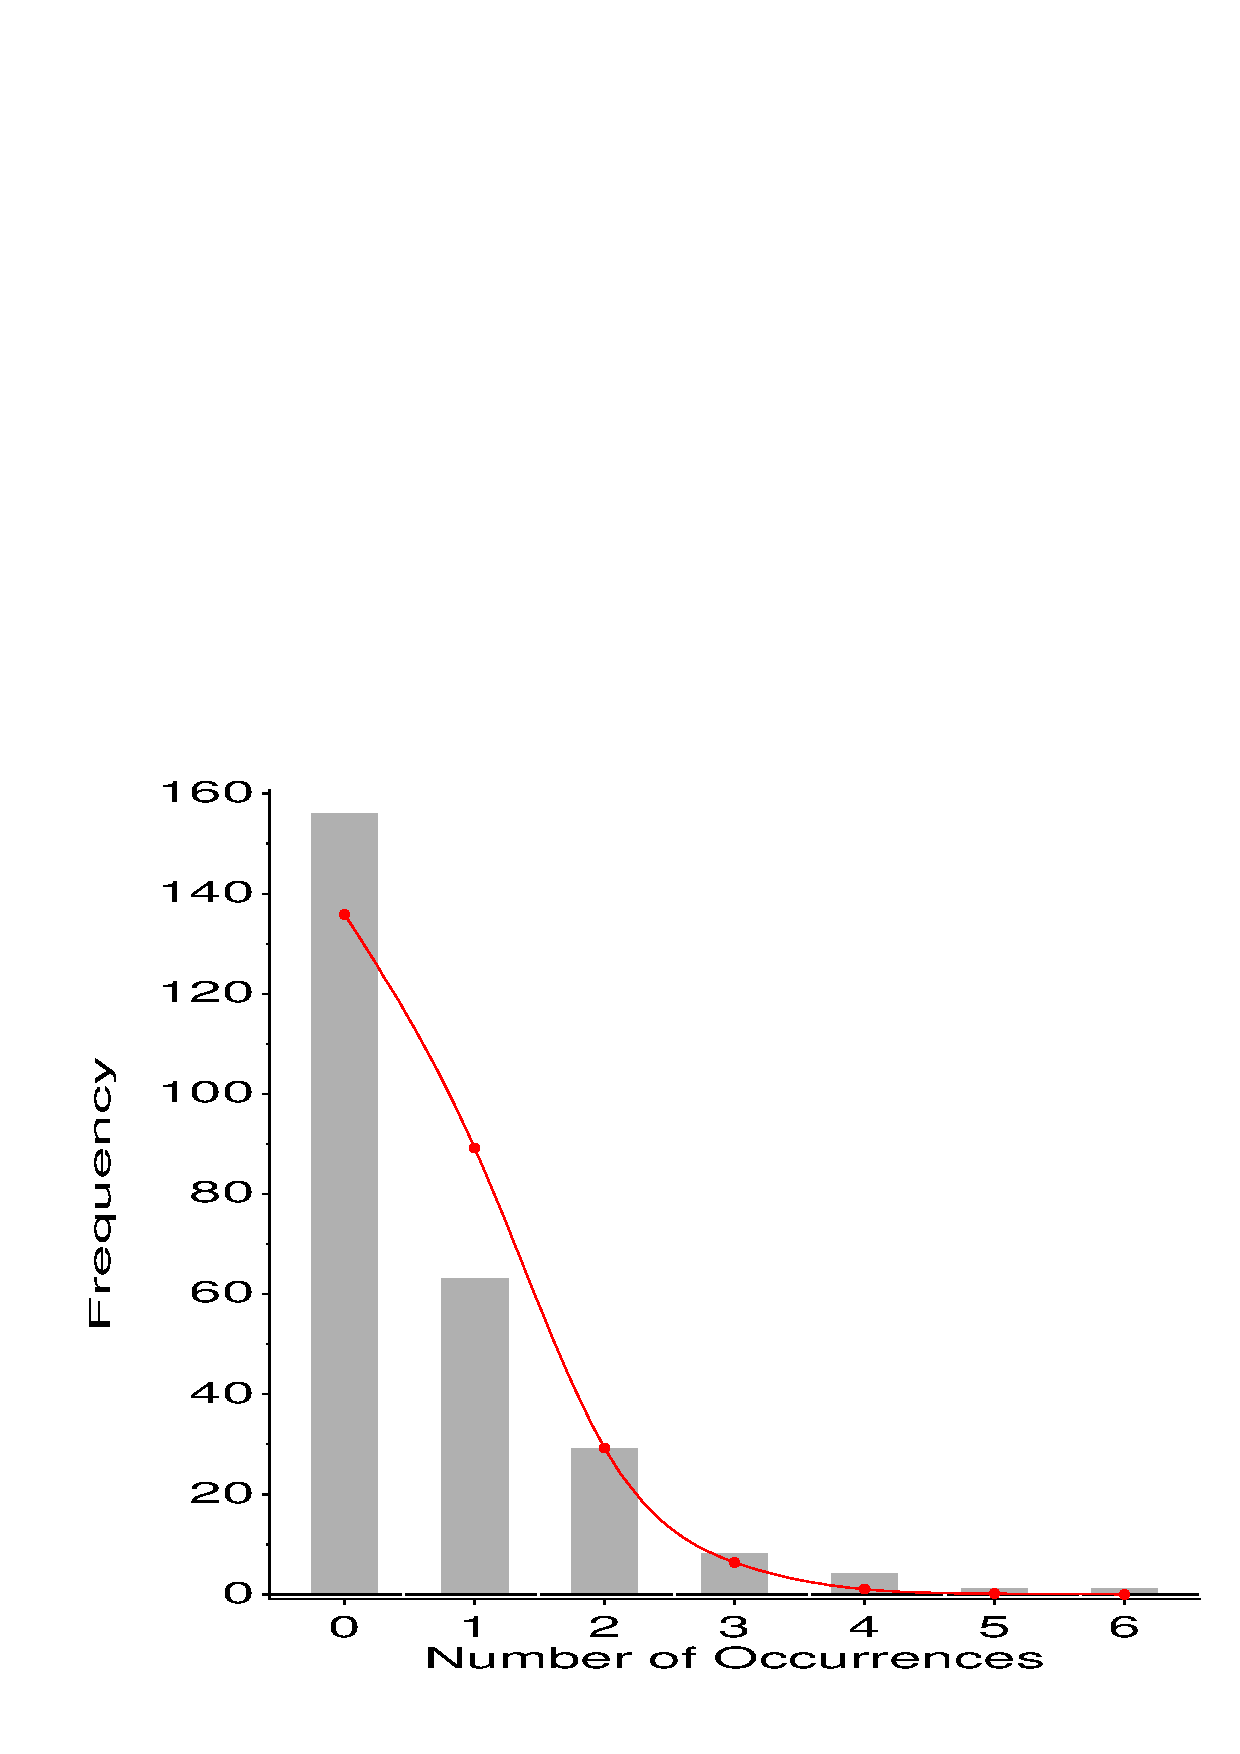
\includegraphics[width=1\linewidth]{fig/madfit1}
 \end{minipage}%
 \hfill
 \begin{minipage}[c]{.49\dispwidth}
 Problems:
	\begin{itemize*}
	\item largest frequencies dominate display
	\item must assess deviations vs. a curve
	\end{itemize*}
 \end{minipage}
	
\end{frame}

\begin{frame}[fragile]
  \frametitle{Hang \& root them $\rightarrow$ Hanging rootograms}
  \citet{Tukey:72,Tukey:77}:
  \begin{itemize*}
  \item shift histogram bars to 
  the fitted curve $\rightarrow$ judge deviations vs. horizontal line.
  \item plot $\sqrt{\mbox{freq}} \rightarrow$
  smaller frequencies are emphasized.
  \end{itemize*}

  \begin{Code}
   %goodfit(data=madison, var=count, freq=blocks, 
     dist=poisson, \sasemph{out=fit});
   \sasemph{%rootgram(data=fit, var=count, obs=blocks);}
  \end{Code}
    \begin{center}
	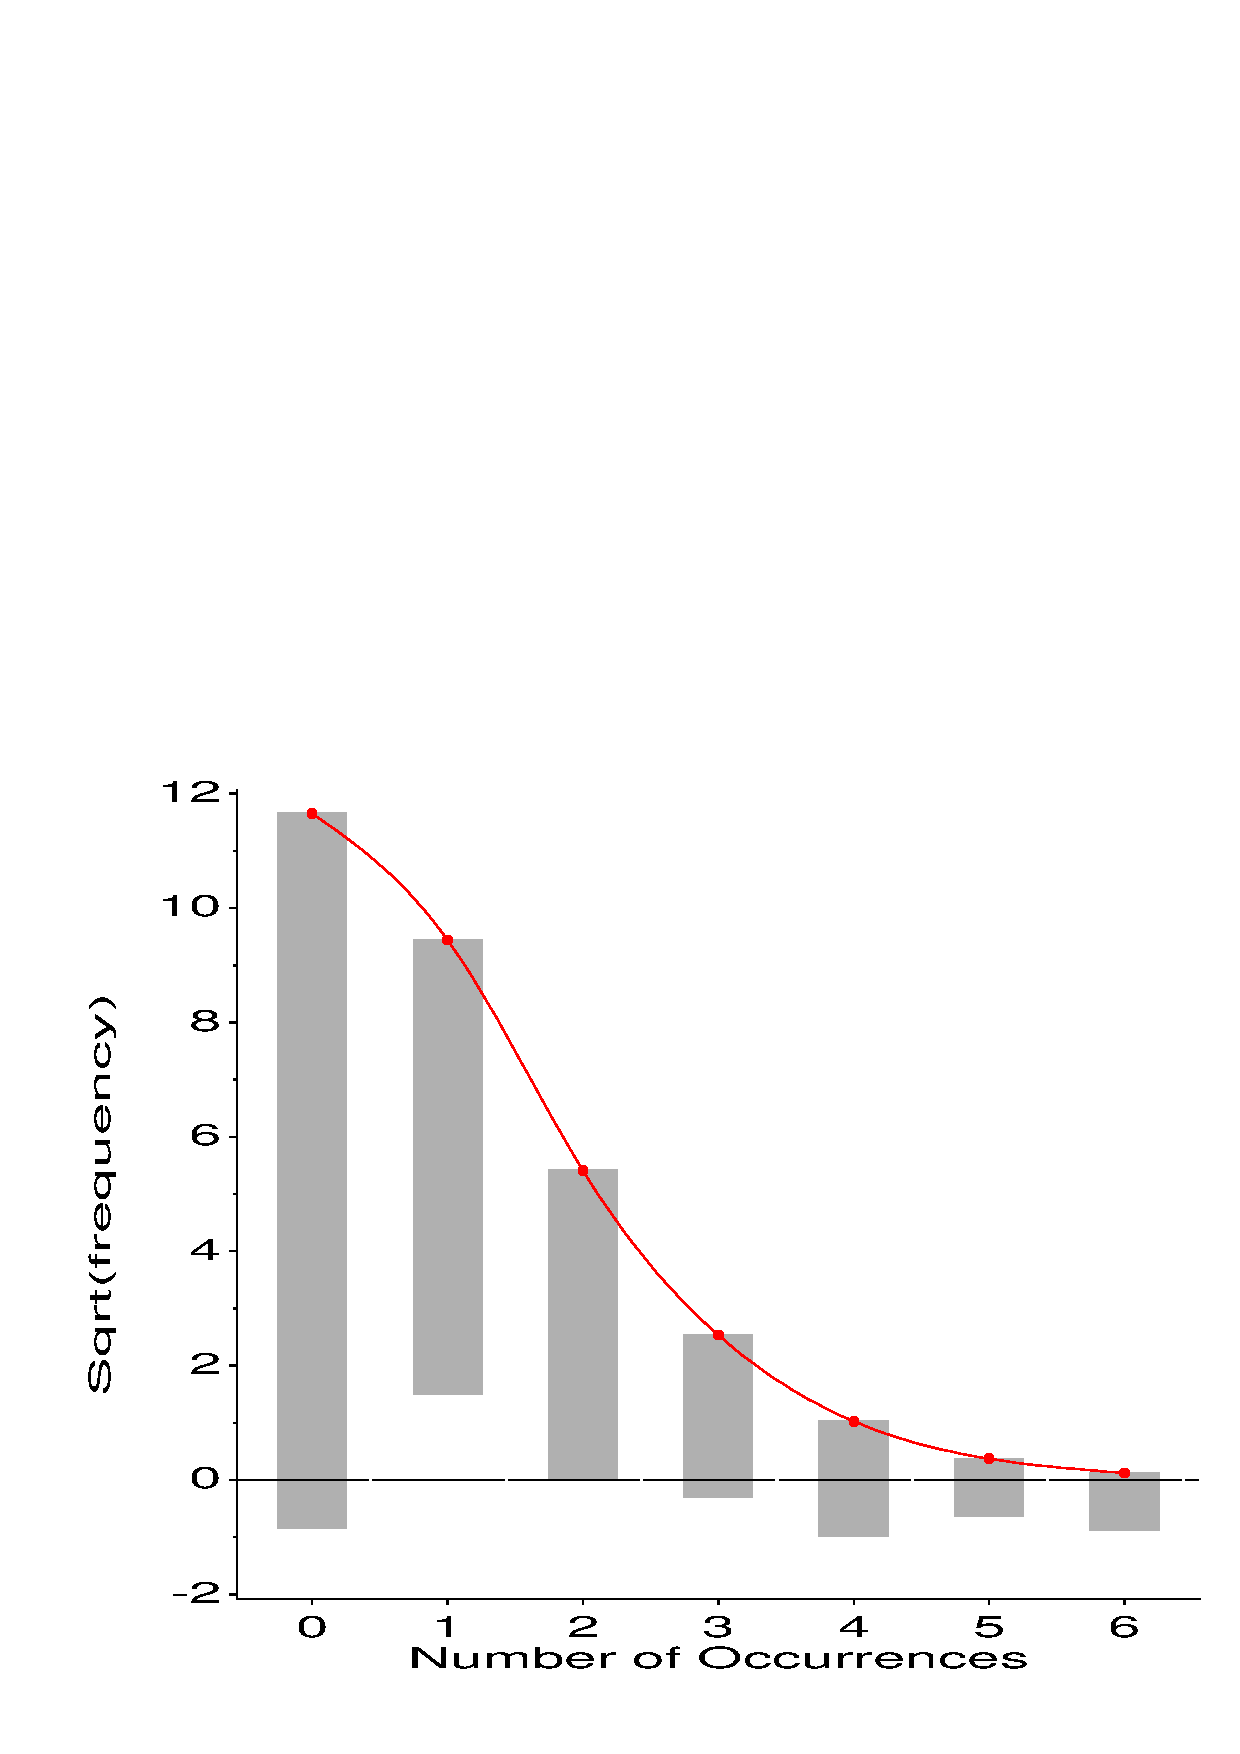
\includegraphics[width=.45\dispwidth,clip]{fig/madfit3}
    \end{center}

\end{frame}

\begin{frame}[fragile]
  \frametitle{Highlight differences $\rightarrow$ Deviation rootograms}
  \begin{itemize*}
  \item Emphasize differences between observed and fitted frequencies
  \item Draw bars to show the gaps (\texttt{btype=dev})
  \end{itemize*}

  \begin{Code}
   %goodfit(data=madison, var=count, freq=blocks, 
     dist=poisson, out=fit);
   %rootgram(data=fit, var=count, obs=blocks, \sasemph{btype=dev});
  \end{Code}
    \begin{center}
	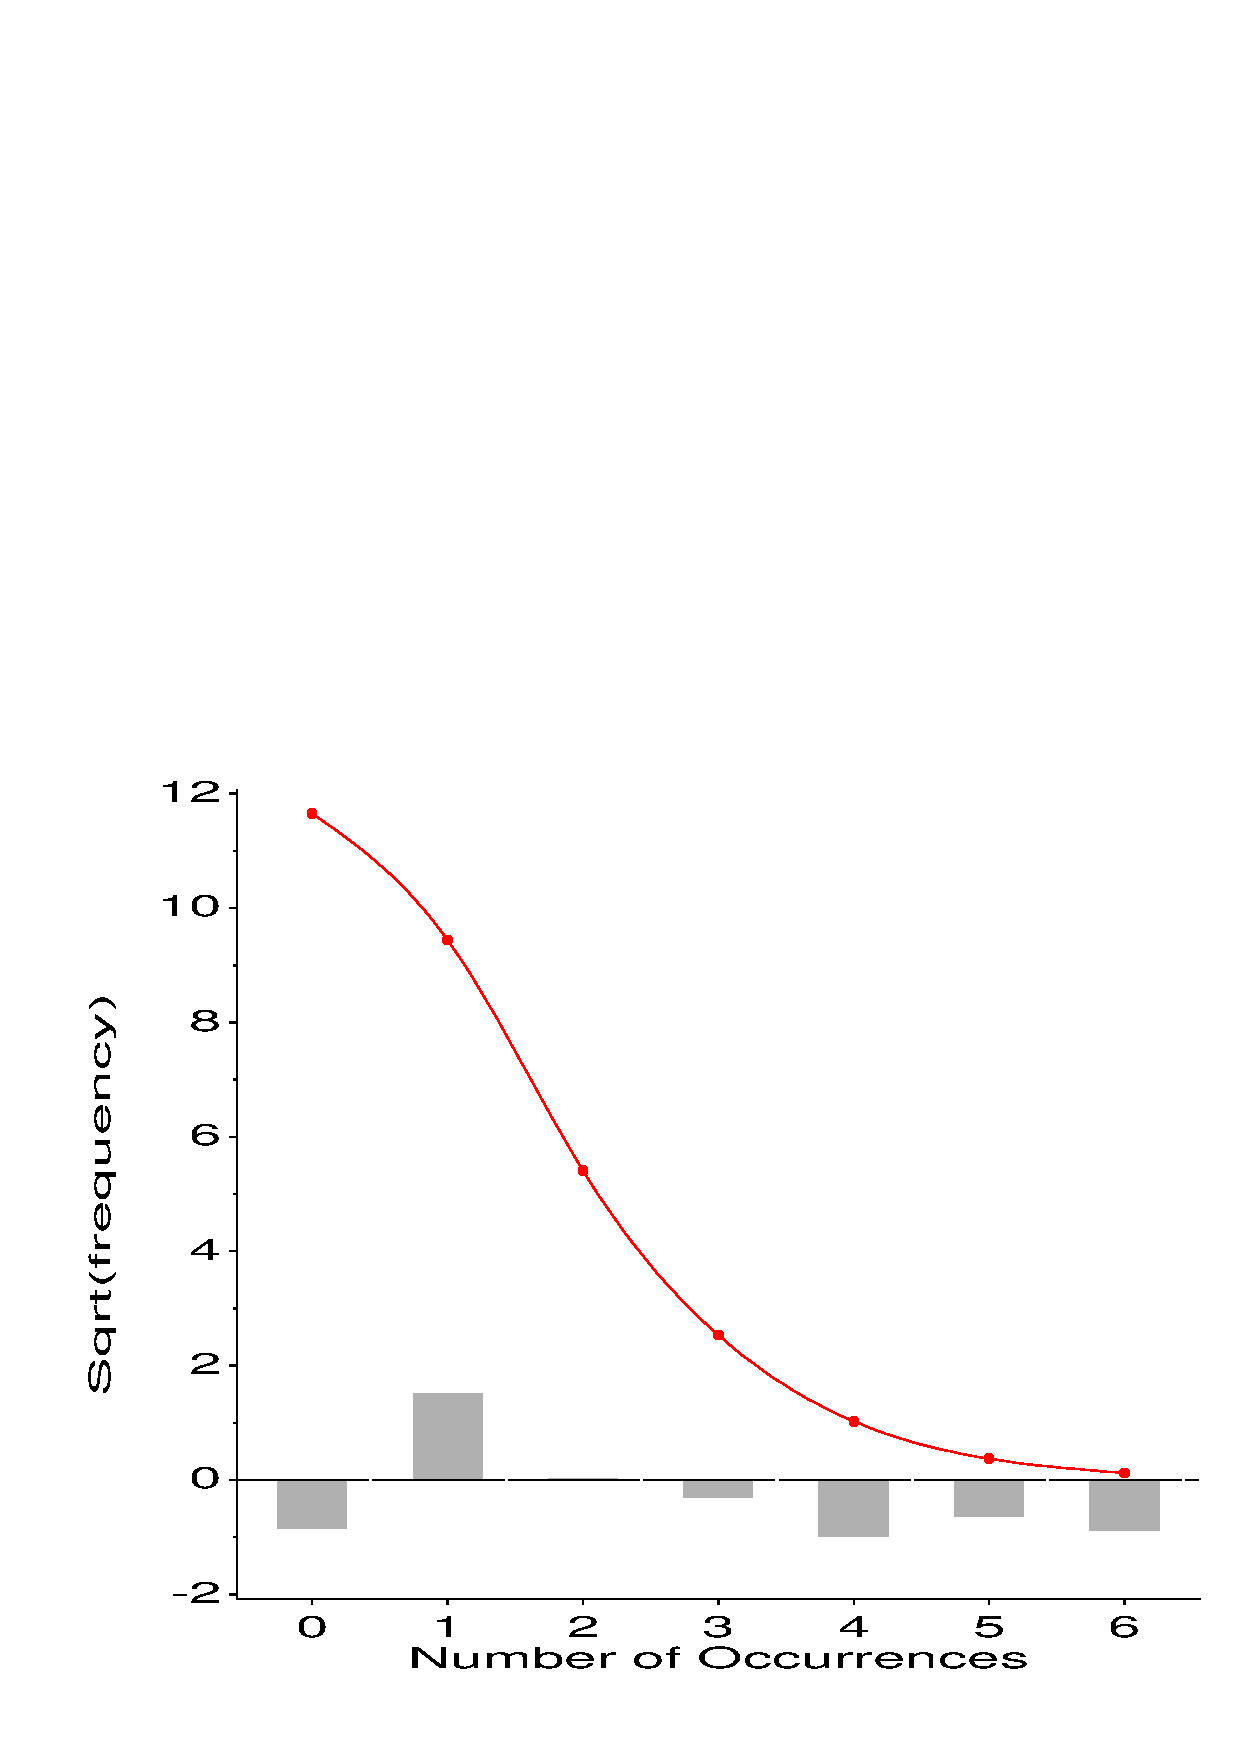
\includegraphics[width=.45\dispwidth,clip]{fig/madfit4}
    \end{center}

\end{frame}

\subsection{Ord plots: diagnose form}
\begin{frame}

\frametitle{Ord plots: Diagnose form of discrete distribution}
\begin{itemize}
\item How to tell which discrete distributions are likely candidates?
\item \citet{Ord:67}: for each of Poisson, Binomial, Negative Binomial, and Logarithmic Series distributions,
	\begin{itemize*}
	\item plot of $k p_k / p_{k-1}$ against $k$ is linear
	\item signs of intercept and slope $\rightarrow$ determine the form,
	give rough estimates of parameters
	\end{itemize*}

\begin{center}
%\vspace{1ex}
\renewcommand{\arraystretch}{.85}
\begin{tabular}{|ccll|}\hline
Slope & Intercept & Distribution & Parameter \\
(b)   & (a)       & (parameter)  &  estimate \\ \hline
0     &  $+$      &  Poisson (\(\lambda\)) & \(\lambda = a\)    \\
$-$   &  $+$      &  Binomial (n, p)       & \(p = b / (b-1)\)  \\
$+$   &  $+$      &  Neg. binomial (n,p)      & \(p = 1 - b\)      \\
$+$   &  $-$      &  Log.\ series (\(\theta\)) & \(\theta =  b\) \\
      &      &                     &   \(\theta = - a\) \\ \hline
\end{tabular}
\end{center}

\item Fit line by WLS, using $\sqrt{n_k-1}$ as weights
\end{itemize}
\end{frame}

\begin{frame}[fragile]
\frametitle{Ord plots}
\begin{itemize}
\item \macro{ORDPLOT}
\begin{Code}
 %ordplot(data=madison, count=Count, freq=blocks);
\end{Code}
\end{itemize}

 \begin{minipage}[c]{.4\dispwidth}
	\begin{itemize*}
	\item Diagnoses distribution as NegBin
	\item Estimates $\hat{p} = 0.576$
	\end{itemize*}
 \end{minipage}
 \hfill
 \begin{minipage}[c]{.59\dispwidth}
  \begin{center}
  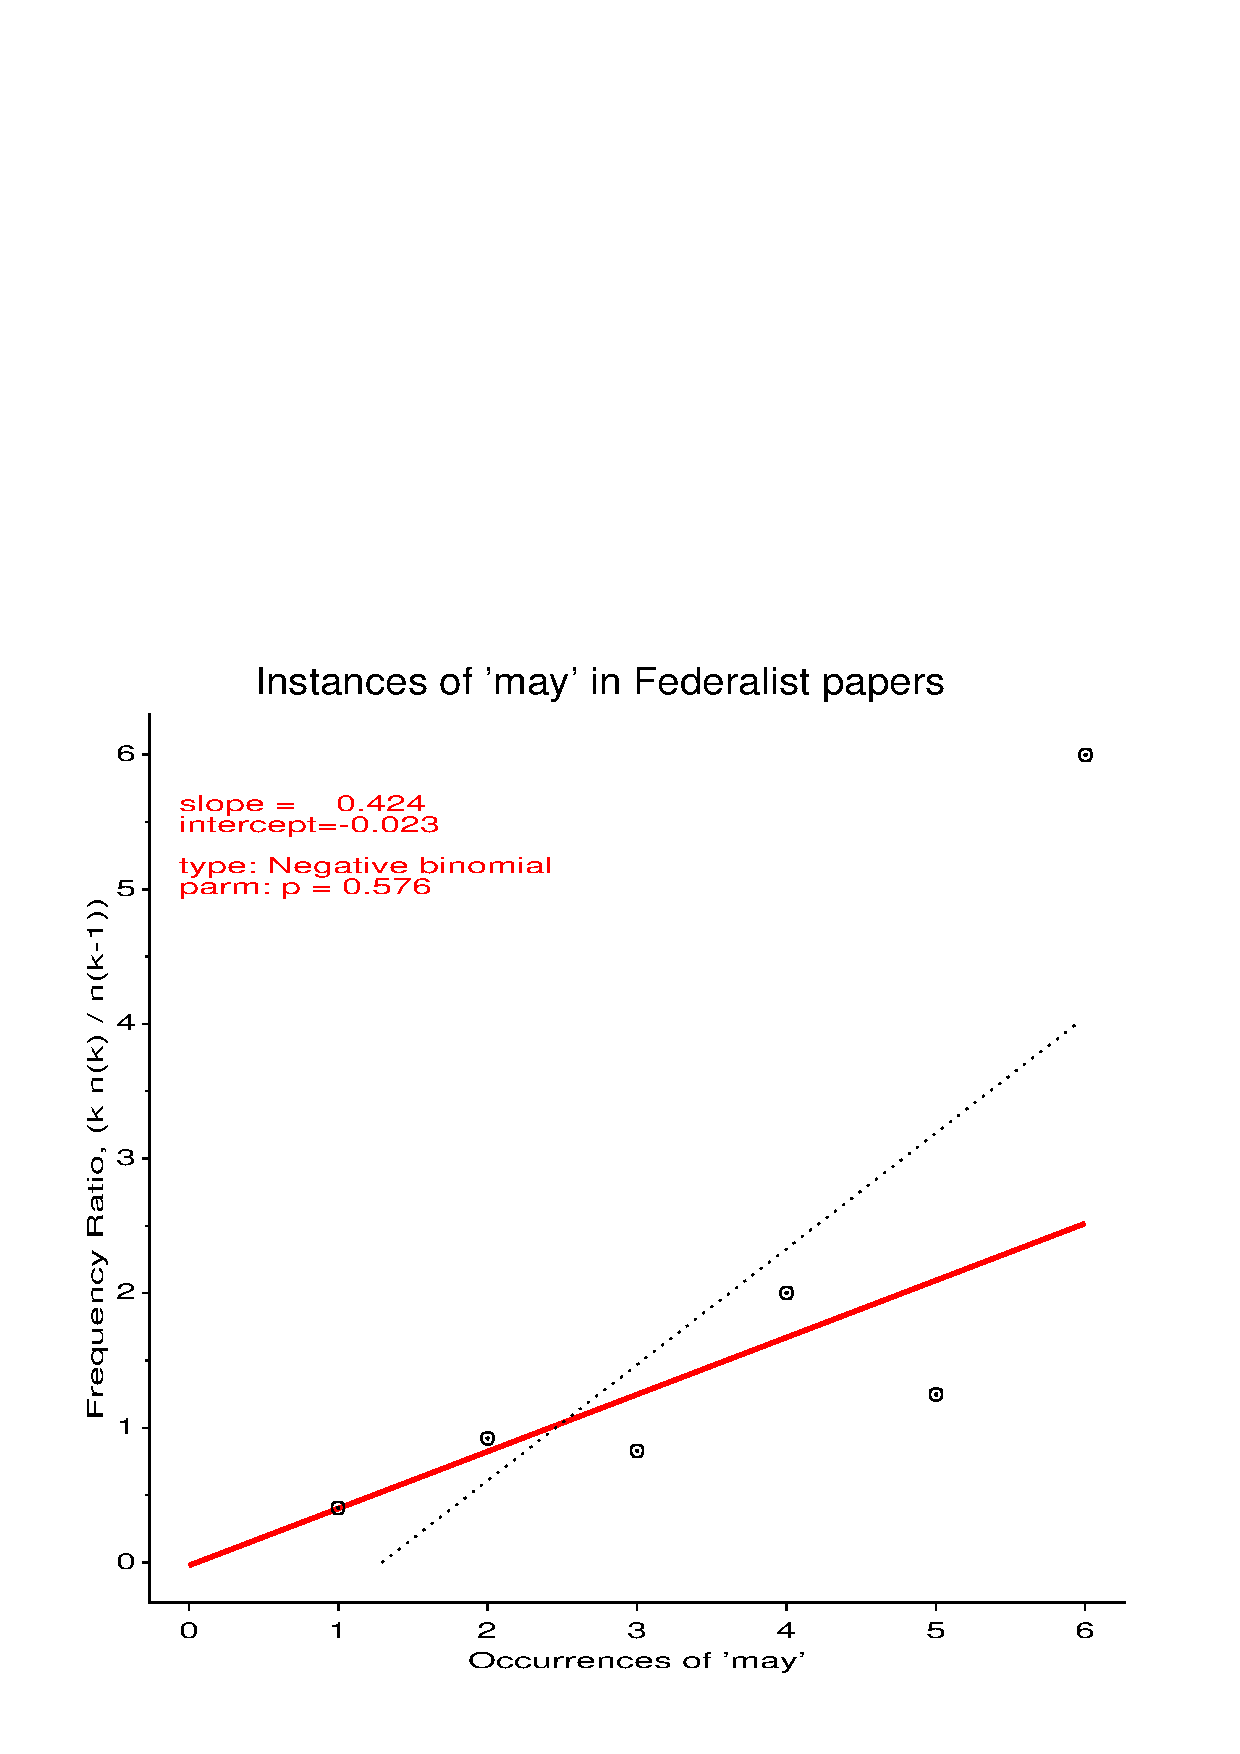
\includegraphics[trim=0 0 0 30,width=\linewidth,clip]{fig/orddemo2}
  \end{center}
 \end{minipage}
\end{frame}
	

\begin{frame}
\frametitle{Ord plots: Other distributions}

 \begin{minipage}[c]{.49\dispwidth}
  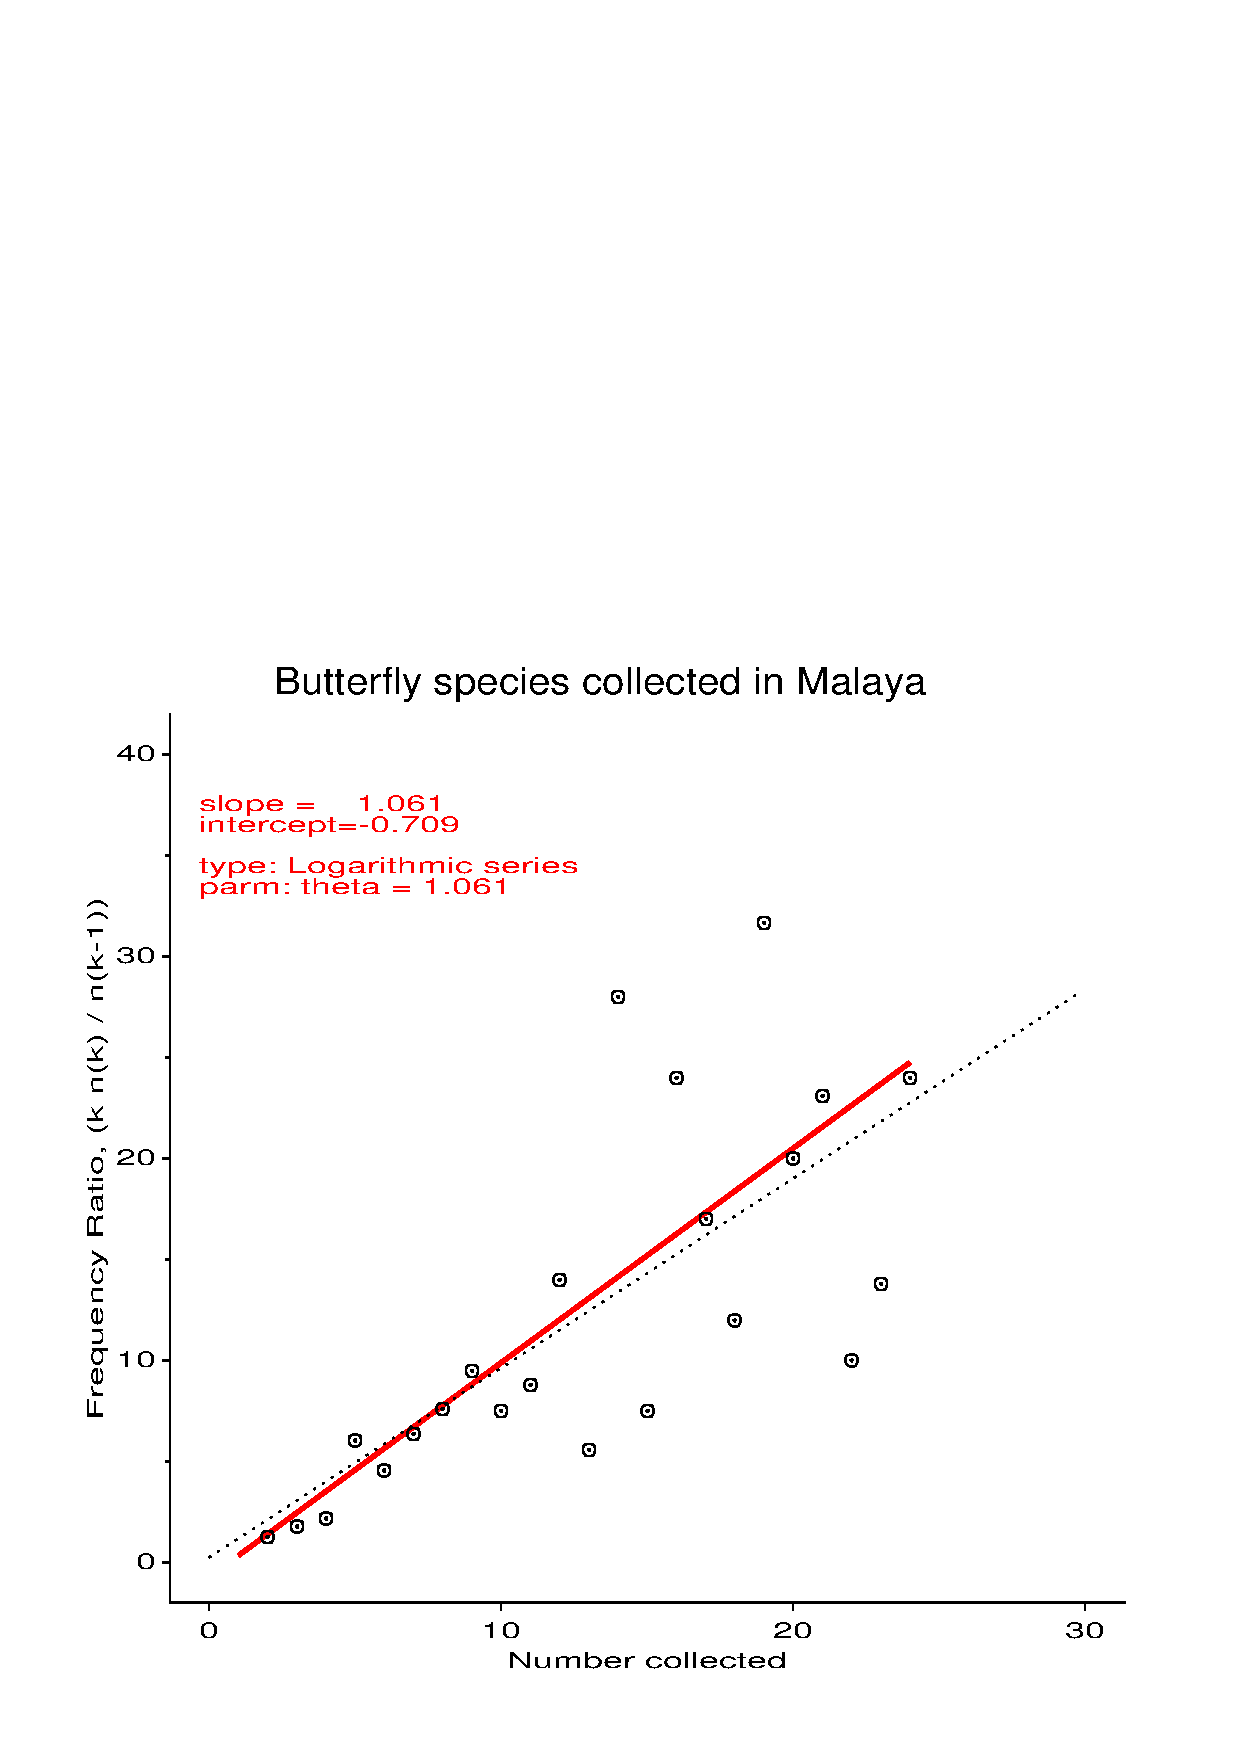
\includegraphics[trim=0 0 0 0,width=\linewidth,clip]{fig/orddemo3}
  \\ \centering Logarithmic series
 \end{minipage}%
 \hfill
 \begin{minipage}[c]{.49\dispwidth}
%  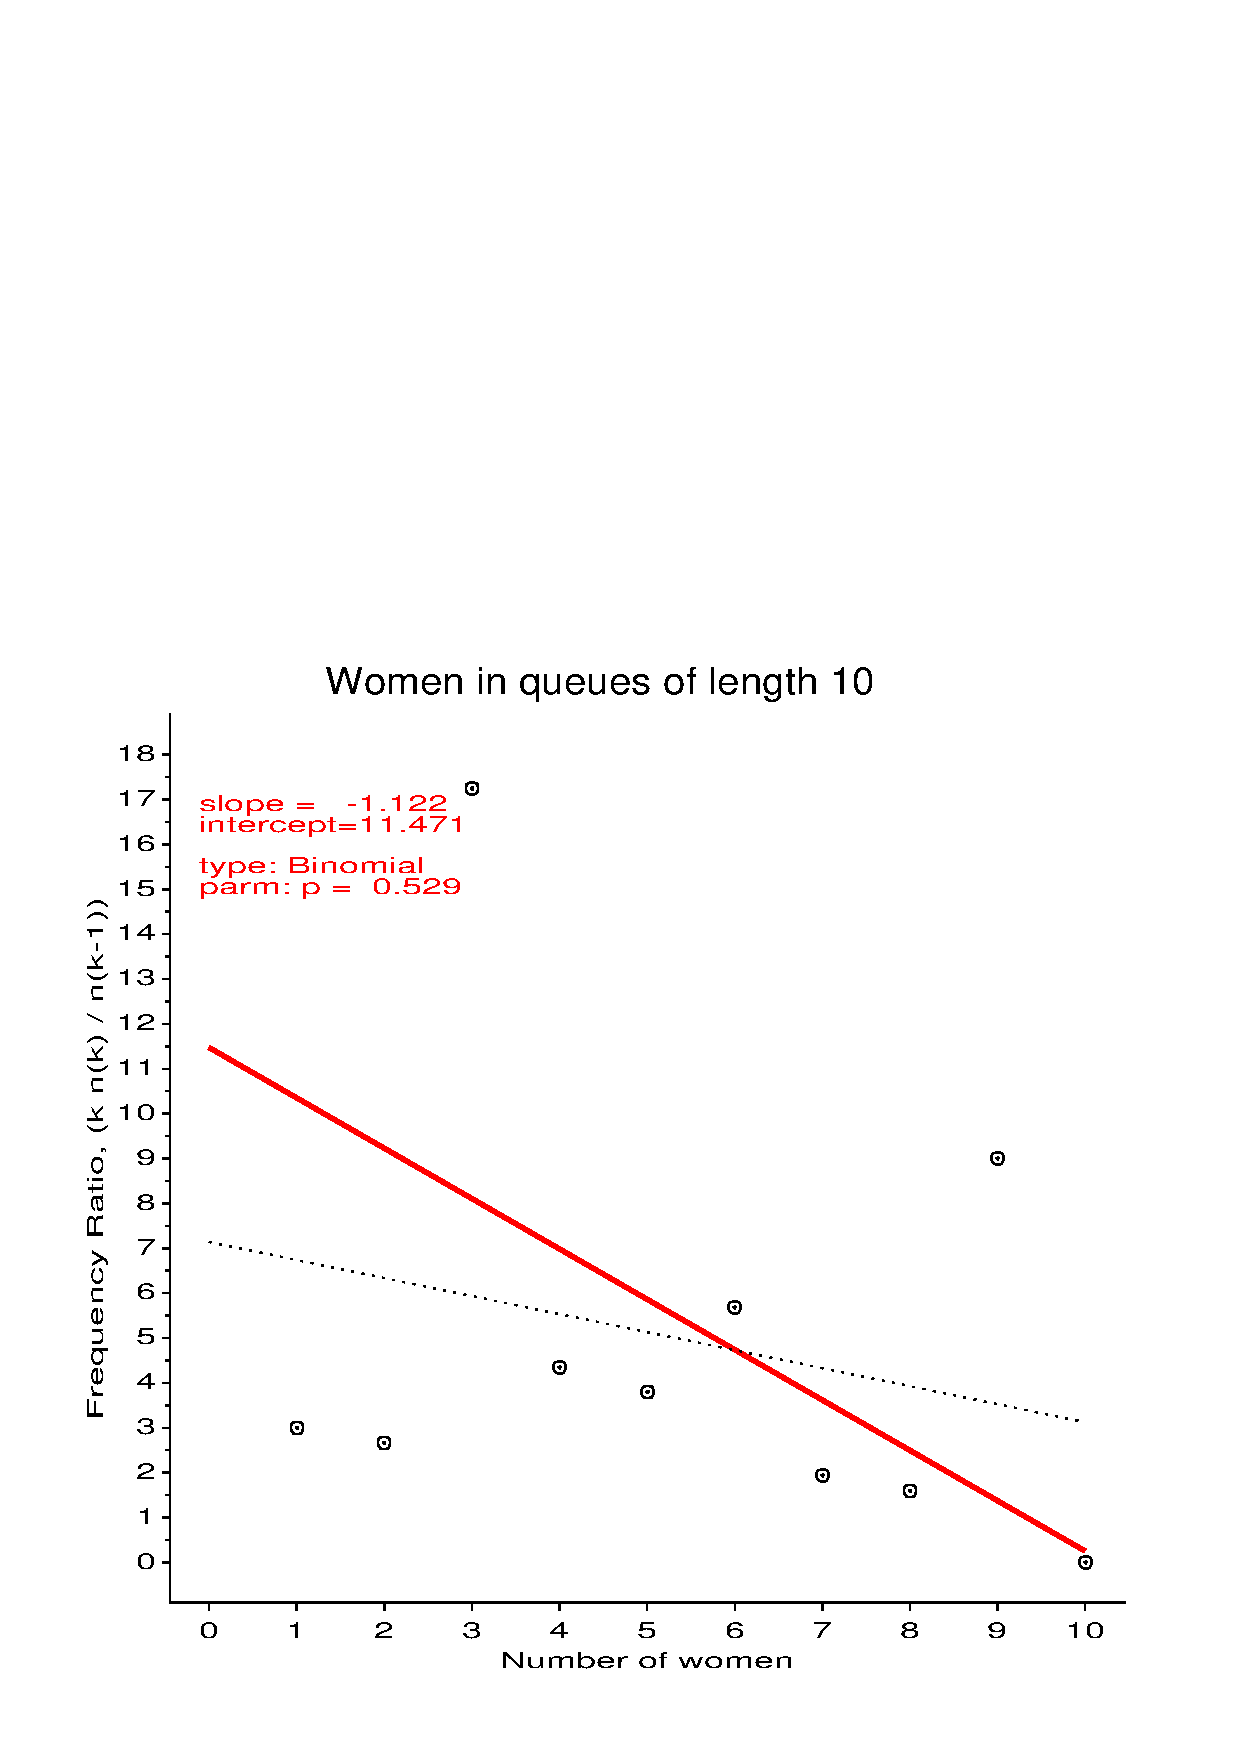
\includegraphics[trim=0 0 0 0,width=\linewidth,clip]{fig/orddemo4}
  \includegraphics[trim=0 0 0 0,width=\linewidth,clip]{fig/saxony4}
  \\ \centering Binomial
 \end{minipage}
\end{frame}

\subsection{Robust distribution plots}
\begin{frame}
  \frametitle{Robust distribution plots: Poisson}
  \begin{itemize}
	\item Ord plots lack robustness 
	\begin{itemize*}
	\item one discrepant freqency, $n_k$
	affects points for both $k$ and $k+1$
	\end{itemize*}

	\item Robust plots for Poisson distribution \citep{HoaglinTukey:85}
	\begin{itemize*}
	  \item For Poisson, plot \boldital{count metameter} =
	  \(\phi \,  ( n_k )  = \log_e ( k ! \,  n_k  /  N )\) vs.\ $k$
	  \item Linear relation $\Rightarrow$ Poisson, slope gives $\hat{\lambda}$
	  \item CI for points, diagnostic (influence) plot
	  \item \macro{POISPLOT}
	\end{itemize*}
  \end{itemize}
\end{frame}

\begin{frame}
  \frametitle{Poissonness plots: Details}
  \begin{itemize}
	\item If the distribution of $n_k$ is Poisson($\lambda$) for some fixed $\lambda$, then each
	observed frequency, $n_k \approx m_k = N p_k$.
	\item Then, setting
\(n_k = N p_k  = { e^{ - \lambda } \:  \lambda^k } /  { k ! }\),
and taking logs of both sides gives
  \[
  \log ( n_k ) = \log \,  N - \lambda  +  k \,  \log \,  \lambda  -
  \log \,  k !
  \]
which can be rearranged to
  \begin{equation*}
  \phi \,  ( n_k )  \equiv \log \left(  \frac{ k ! \:  n_k } {N} \right)
 = - \lambda  +  ( \log \,  \lambda ) \,  k
  \end{equation*}

	\item $\Rightarrow$ if the distribution is Poisson,
	plotting \(\phi ( n_k )\) vs.\ \(k\) should give a line with
	  \begin{itemize*}
	  \item intercept = \(- \lambda\)
	  \item slope = \(\log  \,  \lambda\)
	  \end{itemize*}
	\item Nonlinear relation $\rightarrow$ distribution is \emph{not} Poisson
    \item \citet{HoaglinTukey:85} give details on calculation of confidence intervals
	and influence measures.
  \end{itemize}
\end{frame}

\begin{frame}[fragile]
  \frametitle{\macrot{POISPLOT}: example}
  \begin{Input}[fontsize=\small]
title "Instances of 'may' in Federalist papers";
data madison;
   input count blocks;
   label count='Number of Occurrences'
         blocks='Blocks of Text';
datalines;
  0    156
  1     63
  2     29
  3      8
  4      4
  5      1
  6      1
;
\sasemph{%poisplot(data=madison,count=count, freq=blocks)};
  \end{Input}
\end{frame}

\begin{frame}
  \frametitle{\macrot{POISPLOT}: output}
Curvilinear relation $\rightarrow$ distribution is \emph{not} Poisson
 \begin{minipage}[c]{.49\dispwidth}
  \includegraphics[width=1\linewidth]{fig/poisdemo-mad}
  \\ \centering Poissonness plot
 \end{minipage}%
 \hfill
 \begin{minipage}[c]{.49\dispwidth}
  \includegraphics[width=1\linewidth]{fig/poisdemo-mad3}
  \\ \centering Influence plot for change in $\lambda$
 \end{minipage}

\end{frame}

\begin{frame}[fragile]
  \frametitle{Generalized robust distribution plots}
  Other distributions: Analogous plots, for suitable count metameter, 
  $\phi \,  ( n_k )$
  vs.\ $k$.
  \begin{itemize*}
  \item Linear relation $\Rightarrow$ correct distribution, slope gives parameter estimates
  \item CI reflect variability of the individual counts, $n_k$
  \item \macro{DISTPLOT}
  \end{itemize*}

  \begin{Code}
  %distplot(data=madison, count=count, freq=blocks,
        \sasemph{dist=negbin});
  \end{Code}

  \begin{center}
	\includegraphics[width=.5\dispwidth,clip]{fig/maddist}
  \end{center}
\end{frame}

\subsection{Using R}
\renewcommand{\FileName}{discreteR}

\begin{frame}[fragile]
  \frametitle{Discrete distributions with R and the vcd package}
In R, discrete distributions are conveniently represented as one-way frequency tables,
\begin{Rin}[baselinestretch=0.8]
> library(vcd)
> data(Federalist)
> Federalist
\end{Rin}
\begin{Rout}
nMay
  0   1   2   3   4   5   6 
156  63  29   8   4   1   1 
\end{Rout}
The goodfit() function in vcd fits a variety of discrete distributions:
\begin{Rin}[baselinestretch=0.8]
> # fit the poisson model
> gf1 <- goodfit(Federalist, type="poisson")
> gf1
\end{Rin}
\begin{Rout}[baselinestretch=0.7,fontsize=\footnotesize]
Observed and fitted values for poisson distribution
with parameters estimated by `ML' 

 count observed       fitted
     0      156 135.89138870
     1       63  89.21114067
     2       29  29.28304617
     3        8   6.40799484
     4        4   1.05169381
     5        1   0.13808499
     6        1   0.01510854
\end{Rout}

\end{frame}

\begin{frame}[fragile]
R is object-oriented.  A goodfit object has print(), summary() and plot() methods:
\begin{Rin}
> summary(gf1)
\end{Rin}

\begin{Rout}
         Goodness-of-fit test for poisson distribution

                      X^2 df     P(> X^2)
Likelihood Ratio 25.24312  5 0.0001250511
\end{Rout}

\begin{Rin}
> plot(gf1, main="Federalist data: Poisson fit")
> plot(gf1, main="Federalist data: Poisson fit", type="dev")
\end{Rin}
% two figures
 \begin{minipage}[b]{.5\linewidth}
  \centering
  \includegraphics[width=.95\linewidth]{fig/federalist1}
 \end{minipage}%
 \begin{minipage}[b]{.5\linewidth}
  \centering
  \includegraphics[width=.95\linewidth]{fig/federalist2}
 \end{minipage}

\end{frame}

\begin{frame}[fragile]
  \frametitle{Discrete distributions with R and the vcd package}

The Poisson distribution 
\begin{Rin}
> # In a poisson, mean = var; this is 'over-dispersed'
>  mean(rep(0:6, times=Federalist))
\end{Rin}
\begin{Rout}
[1] 0.6564885
\end{Rout}
\begin{Rin}
>  var(rep(0:6, times=Federalist))
\end{Rin}
\begin{Rout}
[1] 1.007985
\end{Rout}

The negative binomial distribution, Nbin(r, p) 
allows the data to deviate from a true Poisson according to
a parameter $r>0$.
\begin{Rin}
> ## try negative binomial distribution (r, p)
> gf2 <- goodfit(Federalist, type = "nbinomial")
> summary(gf2)
\end{Rin}

\begin{Rout}
         Goodness-of-fit test for nbinomial distribution

                      X^2 df  P(> X^2)
Likelihood Ratio 1.964028  4 0.7423751
\end{Rout}
This has an acceptable fit to the Federalist data

\end{frame}

\begin{frame}[fragile]
  \frametitle{Discrete distributions with R and the vcd package}

Compare the fits side-by-side:
\begin{Rin}
> plot(gf2, main="Federalist data: Negative binomial fit")
> plot(gf1, main="Federalist data: Poisson fit")
\end{Rin}
% two figures
 \begin{minipage}[b]{.5\linewidth}
  \centering
  \includegraphics[width=.95\linewidth]{fig/federalist3}
 \end{minipage}%
 \begin{minipage}[b]{.5\linewidth}
  \centering
  \includegraphics[width=.95\linewidth]{fig/federalist1}
 \end{minipage}

{\large\bfseries Conclusions:}
\begin{itemize*}
  \item Perhaps marker words like 'may' do not occur with constant probability in all
  blocks of text
  \item Perhaps the blocks of text were written under different circumstances
\end{itemize*}

\begin{comment}
> # geometric = NBin (1,p)
> gf3 <- goodfit(Federalist, type = "nbinomial", par = list(size = 1))
> summary(gf3)

\begin{Rout}
         Goodness-of-fit test for nbinomial distribution

                      X^2 df  P(> X^2)
Likelihood Ratio 2.294143  5 0.8071267
\end{Rout}
> plot(gf3, main="Federalist data: Geometric distribution, NBin(1,p)")
\end{comment}

\end{frame}

\begin{frame}[fragile]
vcd includes Ord\_plot() and distplot() functions. E.g.,
\begin{Rin}
> Ord_plot(Federalist, 
       main = "Instances of 'may' in Federalist papers")
\end{Rin}
  \begin{center}
        \includegraphics[width=.72\dispwidth,clip]{fig/federalist5}
  \end{center}

\end{frame}


\section{Testing association}
\renewcommand{\FileName}{assoc}
\subsection{Nominal factors}
\begin{frame}[fragile]
  \frametitle{Testing Association in Two-Way Tables}
  \begin{block}{\large\bfseries Typical analysis: Nominal factors}
  \end{block}
      \begin{itemize}
	  \item Pearson $\chisq$ (or LR $\chisq$)--- when most expected
	  frequencies $\ge 5$.

\begin{listing}[frame=single]
proc freq;
   weight count;        \sascomment{/* if in frequency form */}
   table factor * response / \sasemph{chisq}; 
\end{listing}

	  \item Exact tests--- small tables, small sample sizes (e.g., Fisher's)

\begin{listing}[frame=single]
proc freq;
   weight count;        \sascomment{/* if in frequency form */}
   table factor * response / \sasemph{chisq};
   \sasemph{exact pchi;}
\end{listing}
	  \end{itemize}
\end{frame}

\begin{frame}[fragile]
  \frametitle{Example: Cholesterol diet and heart disease}
Is there a relation between Hi/Lo cholesterol diet and heart disease?
\vspace{2ex}

\begin{Input}[fontsize=\footnotesize,label=\fbox{\texttt{fat.sas}},baselinestretch=0.8]
title 'Cholesterol diet and heart disease';
data fat;
   input diet $ disease $ count;
datalines;
LoChol  No   6
LoChol  Yes  2
HiChol  No   4
HiChol  Yes 11
;

proc freq data=fat;
  weight count;
  tables diet * disease / chisq nopercent nocol;
  \sasemph{exact pchi};
\end{Input}
\end{frame}

\begin{frame}[fragile]
Standard output:
\begin{Output}[fontsize=\footnotesize,gobble=7,baselinestretch=.7]
                           Table of diet by disease

                     diet      disease

                     Frequency|
                     Row Pct  |No      |Yes     |  Total
                     ---------+--------+--------+
                     HiChol   |      4 |     11 |     15
                              |  26.67 |  73.33 |
                     ---------+--------+--------+
                     LoChol   |      6 |      2 |      8
                              |  75.00 |  25.00 |
                     ---------+--------+--------+
                     Total          10       13       23


                   Statistics for Table of diet by disease

            Statistic                     DF       Value      Prob
            ------------------------------------------------------
            Chi-Square                     1      4.9597    0.0259
            Likelihood Ratio Chi-Square    1      5.0975    0.0240
            Continuity Adj. Chi-Square     1      3.1879    \sasemph{0.0742}

         \sasemph{WARNING}: 50% of the cells have expected counts less than 5. 
                  (Asymptotic) Chi-Square may not be a valid test.
\end{Output}
\begin{itemize*}
  \item The Pearson and LR $\chisq$ tests are \emph{not valid}--- sample size too small
  \item The conservative continuity-adjusted test fails significance
\end{itemize*}
\end{frame}

\begin{frame}[fragile]
\begin{itemize*}
  \item Exact tests are \emph{valid} and significant.
\end{itemize*}
Exact test output:
\begin{Output}[fontsize=\footnotesize,gobble=7,baselinestretch=.8]
            		   Pearson Chi-Square Test
        		  ----------------------------------
        		  Chi-Square                  4.9597
        		  DF                               1
        		  Asymptotic Pr >  ChiSq      0.0259
        		  Exact      Pr >= ChiSq      0.0393


                		 Fisher's Exact Test
        		  ----------------------------------
        		  Cell (1,1) Frequency (F)         4
        		  Left-sided Pr <= F          0.0367
        		  Right-sided Pr >= F         0.9967

        		  Table Probability (P)       0.0334
        		  Two-sided Pr <= P           \sasemph{0.0393}
\end{Output}

\end{frame}

\begin{frame}[fragile]
  \frametitle{Preview: Visualizing association in 2 $\times$ 2 tables}
 \begin{minipage}[c]{.5\linewidth}
  \centering
  \includegraphics[width=.9\linewidth,clip]{fig/fat2}
 \end{minipage}%
 \begin{minipage}[c]{.5\linewidth}
   \begin{itemize}
    \item Fourfold display: area $\sim$ frequency
    \item Color: \blue{blue} ($+$), \red{red}($-$)
    \item Confidence bands: significance of odds ratio
    \item Interp: Hi cholesterol $\rightarrow$ Heart disease
   \end{itemize}
 \end{minipage}
\vspace{1ex}
\begin{listing}[frame=single]
%ffold(data=fat, var=diet disease);
\end{listing}

\end{frame}

\subsection{Ordinal factors and Stratified analyses}
\begin{frame}[fragile]
  \frametitle{Ordinal factors and Stratified analyses}

  \begin{block}{\large\bfseries More powerful CMH tests}
      \begin{itemize*}
	  \item When either the row (factor) or column (response) levels are
	  \alert{ordered}, more specific (CMH = Cochran - Mantel - Haentzel) tests
	  which take order into account have greater power to detect ordered
	  relations.
\begin{listing}[frame=single]
proc freq;
   weight count;
   table factor * response / chisq \sasemph{cmh}; 
\end{listing}
	  \end{itemize*}
  \end{block}
  \begin{block}{\large\bfseries Control for other background variables} 
      \begin{itemize*}
	    \item Stratified analysis tests the association between a main
		factor and response \emph{within}  levels of the control
		variable(s)
		\item Can also test for homogeneous association across strata
\begin{listing}[frame=single]
proc freq;
   weight count;
   table \sasemph{strata} * factor * response / chisq \sasemph{cmh}; 
\end{listing}
	  \end{itemize*}
  \end{block}
\end{frame}

% slide template
\begin{frame}[fragile]
  \frametitle{Example: Arthritis treatment}
  Data on treatment for rheumatoid arthritis \citep{KochEdwards:88}
  \begin{itemize}
	\item {\large\bfseries Ordinal response}: none, some, or marked improvement
	\item {\large\bfseries Factor}:  active treatment vs.\ placebo
	\item{\large\bfseries Strata}:  Sex
  \end{itemize}
\begin{listing}
                      |         Outcome
   ---------+---------+--------------------------+
   Treatment|  Sex    |None    |Some    |Marked  |  Total
   ---------+---------+--------+--------+--------+
   Active   |  Female |      6 |      5 |     16 |     27
            |  Male   |      7 |      2 |      5 |     14
   ---------+---------+--------+--------+--------+
   Placebo  |  Female |     19 |      7 |      6 |     32
            |  Male   |     10 |      0 |      1 |     11
   ---------+---------+--------+--------+--------+
   Total                    42       14       28       84
\end{listing}
\end{frame}

\begin{frame}[fragile]
{\bfseries Overall analysis, ignoring sex}:
\begin{Input}[fontsize=\footnotesize,label=\fbox{\texttt{arthfreq.sas} $\cdots$},baselinestretch=0.8]
title 'Arthritis Treatment: PROC FREQ Analysis';
data arth;
   input sex$ treat$ @;
   do improve = 'None  ', 'Some', 'Marked';
      input count @;
      output;
      end;
datalines;
Female  Active    6  5  16
Female  Placebo  19  7   6
Male    Active    7  2   5
Male    Placebo  10  0   1
;
\sascomment{*-- Ignoring sex;}
proc freq \sasemph{order=data};
   weight count;
   tables treat * improve / \sasemph{cmh} chisq nocol nopercent;
   run;
\end{Input}
{\bfseries Notes}:

\begin{itemize*}

  \item \PROC{FREQ} orders character variables alphabetically (i.e., `Marked', `None', `Some') by
   default.  
  \item To treat the IMPROVE variable as
   ordinal, use \alert{\texttt{order=data}} on the \PROC{FREQ}
   statement.

%  \item The \opt{chisq}{FREQ} gives the usual \(\chi^2\) tests
%   (Pearson, Fisher's, etc.).  The \opt{cmh}{FREQ} requests the
%   \IX{Cochran-Mantel-Haenszel tests} for ordinal variables.
\end{itemize*}
\end{frame}

\begin{frame}[fragile]
\bfseries{Overall analysis, ignoring sex}: Results (\texttt{chisq} option)
\begin{Output}[gobble=2]
             STATISTICS FOR TABLE OF TREAT BY IMPROVE

      Statistic                     DF     Value        Prob
      ------------------------------------------------------
      Chi-Square                     2    13.055       0.001
      Likelihood Ratio Chi-Square    2    13.530       0.001
      Mantel-Haenszel Chi-Square     1    12.859       0.000
      Phi Coefficient                      0.394
      Contingency Coefficient              0.367
      Cramer's V                           0.394
\end{Output}
Cochran-Mantel-Haenszel tests: (\texttt{cmh} option)
\begin{Output}[gobble=4]
               SUMMARY STATISTICS FOR TREAT BY IMPROVE
      Cochran-Mantel-Haenszel Statistics (Based on Table Scores)

    Statistic   Alternative Hypothesis    DF       Value      Prob
    --------------------------------------------------------------
       1        Nonzero Correlation        1      12.859     0.000
       2        Row Mean Scores Differ     1      12.859     0.000
       3        General Association        2      12.900     0.002
\end{Output}
\end{frame}

\subsection{CMH tests for ordinal variables}
\begin{frame}
\frametitle{CMH tests for ordinal variables}
Three types of test:
  \begin{block}{\large\bfseries Non-zero correlation} 
	  \begin{itemize*}
	  \item Use when \emph{both} row and column variables are ordinal.
	  \item CMH \(\chi^2 = ( N - 1) r^2\), assigning scores (1, 2, 3, ...)
	  \item most powerful for \emph{linear} association
	  \end{itemize*}
  \end{block}
  \begin{block}{\large\bfseries Row Mean Scores Differ} 
      \begin{itemize*}
	  \item Use when only \emph{column} variable is ordinal
	  \item Analogous to the Kruskal-Wallis non-parametric test (ANOVA on rank scores)
	  \item Ordinal variable must be listed \alert{last} in the \texttt{TABLES} statement
       \end{itemize*}
  \end{block}
  \begin{block}{\large\bfseries General Association} 
      \begin{itemize*}
	  \item Use when \emph{both} row and column variables are nominal.
	  \item Similar to overall Pearson \(\chi^2\) and Likelihood Ratio \(\chi^2\).
       \end{itemize*}
  \end{block}
\end{frame}

\begin{frame}[fragile,t]
  \frametitle{Sample CMH Profiles}
  \boldital{Only general association:}
\begin{listing}
        | b1    | b2    | b3    | b4    | b5    |  Total  Mean
--------+-------+-------+-------+-------+-------+
  a1    |     0 |    15 |    25 |    15 |     0 |     55   3.0
  a2    |     5 |    20 |     5 |    20 |     5 |     55   3.0
  a3    |    20 |     5 |     5 |     5 |    20 |     55   3.0
--------+-------+-------+-------+-------+-------+
Total        25      40      35      40      25      165
\end{listing}
\vspace{2ex}
Output:
\begin{Output}[gobble=4]
      Cochran-Mantel-Haenszel Statistics (Based on Table Scores)

    Statistic   Alternative Hypothesis    DF       Value      Prob
    --------------------------------------------------------------
       1        Nonzero Correlation        1       0.000     1.000
       2        Row Mean Scores Differ     2       0.000     1.000
       3        General Association        8      91.797     \sasemph{0.000}
\end{Output}
\end{frame}

\begin{frame}[fragile,t]
  \frametitle{Sample CMH Profiles}
\boldital{Linear Association:}

\begin{listing}
        | b1    | b2    | b3    | b4    | b5    |  Total   Mean
--------+-------+-------+-------+-------+-------+
  a1    |     2 |     5 |     8 |     8 |     8 |     31   3.48
  a2    |     2 |     8 |     8 |     8 |     5 |     31   3.19
  a3    |     5 |     8 |     8 |     8 |     2 |     31   2.81
  a4    |     8 |     8 |     8 |     5 |     2 |     31   2.52
--------+-------+-------+-------+-------+-------+
Total        17      29      32      29      17      124
\end{listing}
\vspace{2ex}
Output:
\begin{Output}[gobble=4]
      Cochran-Mantel-Haenszel Statistics (Based on Table Scores)

    Statistic   Alternative Hypothesis    DF       Value      Prob
    --------------------------------------------------------------
       1        Nonzero Correlation        1      10.639     \sasemph{0.001}
       2        Row Mean Scores Differ     3      10.676     \sasemph{0.014}
       3        General Association       12      13.400     0.341
\end{Output}
\end{frame}

\begin{frame}
  \frametitle{Sample CMH Profiles}
\boldital{Visualizing Association:} Sieve diagrams

\vspace{2ex}
 \begin{minipage}[b]{.5\linewidth}
  \centering
  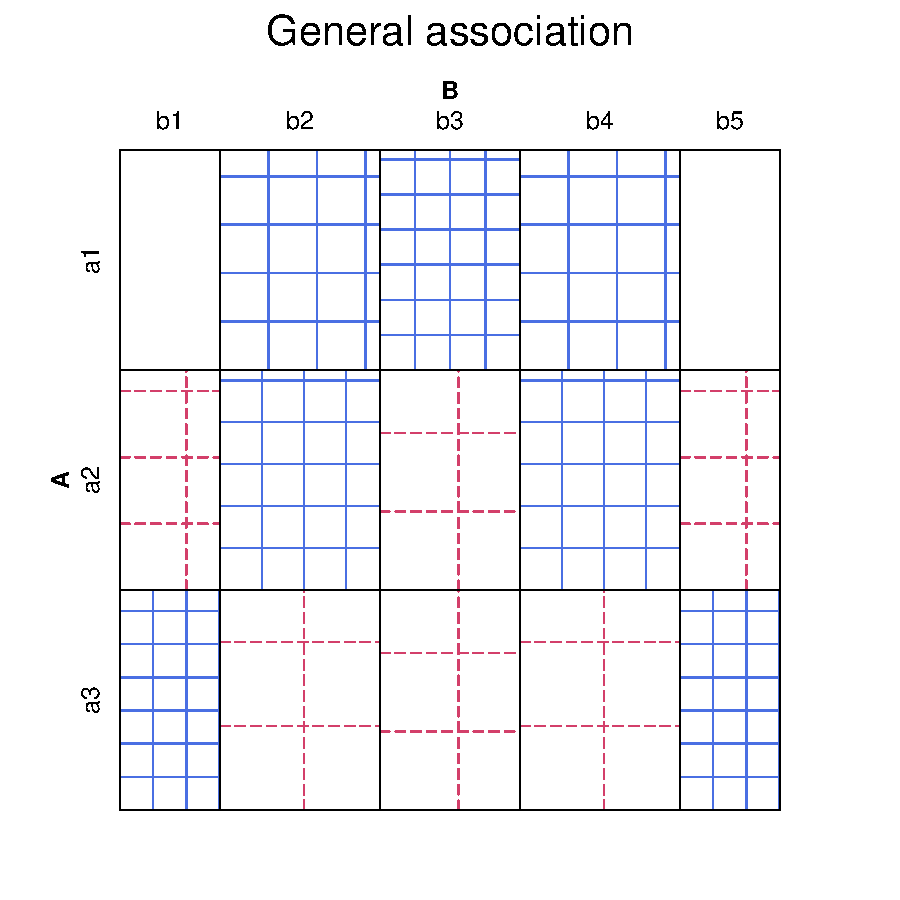
\includegraphics[width=.95\linewidth]{fig/cmhdemo1}
%  \caption{General association (sieve diagram)}\label{fig:cmhdemo1}
 \end{minipage}%
 \begin{minipage}[b]{.5\linewidth}
  \centering
  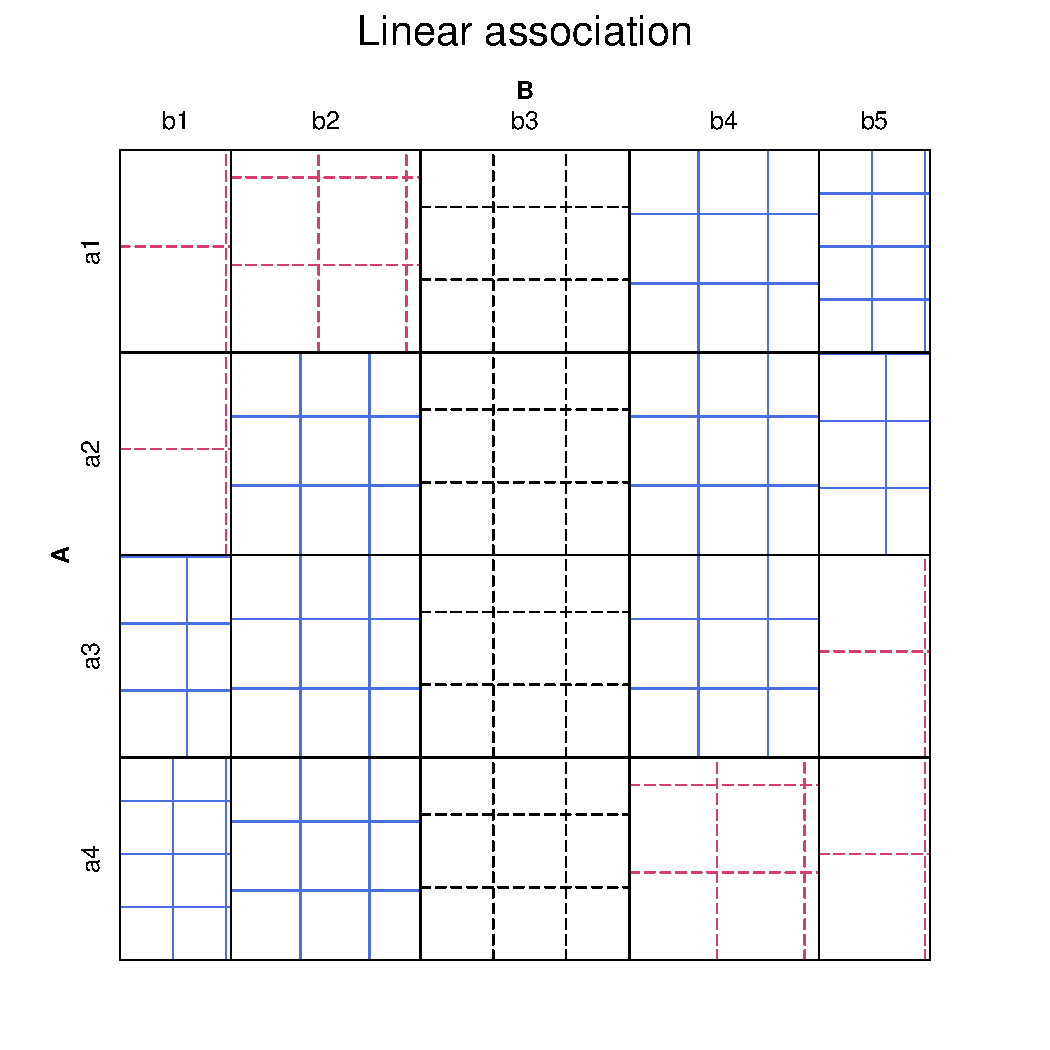
\includegraphics[width=.95\linewidth]{fig/cmhdemo2}
%  \caption{Linear association (sieve diagram)}\label{fig:cmhdemo2}
 \end{minipage}
\end{frame}

\subsection{Stratified analysis}
\begin{frame}[fragile]
  \frametitle{Stratified analysis}
  \begin{block}{\large\bfseries Overall analysis}
      \begin{itemize*}
	  \item ignores other variables (like sex), by collapsing over them
	  \item risks losing important interactions (e.g., different associations for M \& F)
	  \end{itemize*}
  \end{block}
  \begin{block}{\large\bfseries Stratified analysis}
      \begin{itemize*}
	  \item controls for the effects of one or more background variables
	  \item list stratification variable(s) \emph{first} on the \texttt{TABLES} statement
\begin{listing}[frame=single]
proc freq;
   tables \sasemph{age * sex} * treat * improve;
\end{listing}
	  \end{itemize*}
  \end{block}
  \begin{block}{Looking forward: Loglinear models}
      \begin{itemize*}
	  \item allow more general hypotheses to be stated and tested
	  \item closer connection between testing and visualization (\alert{how} are variables associated)
 	  \end{itemize*}
 \end{block}
\end{frame}

\begin{frame}[fragile]
  \frametitle{Stratified analysis}
The statements below request a stratified analysis with CMH tests,
controlling for sex.

\begin{Input}[fontsize=\footnotesize,label=\fbox{$\cdots$ \texttt{arthfreq.sas} $\cdots$},baselinestretch=0.8,firstnumber=20]
\sascomment{*-- Stratified analysis, controlling for sex;}
proc freq order=data;
   weight count;
   tables sex * treat * improve / cmh chisq nocol nopercent;
   run;
\end{Input}
$\rightarrow$ separate tables (partial tests) for Females and Males
\begin{Output}
       STATISTICS FOR TABLE 1 OF TREAT BY IMPROVE
               CONTROLLING FOR SEX=Female

 Statistic                     DF     Value        Prob
 ------------------------------------------------------
 Chi-Square                     2    11.296       0.004
 Likelihood Ratio Chi-Square    2    11.731       0.003
 Mantel-Haenszel Chi-Square     1    10.935       0.001
  ...
\end{Output}
\begin{itemize*}
\item Strong association between TREAT and IMPROVE for females
\end{itemize*}
\end{frame}

\begin{frame}[fragile]
Males:
\begin{Output}
       STATISTICS FOR TABLE 2 OF TREAT BY IMPROVE
                CONTROLLING FOR SEX=Male

 Statistic                     DF     Value        Prob
 ------------------------------------------------------
 Chi-Square                     2     4.907       0.086
 Likelihood Ratio Chi-Square    2     5.855       0.054
 Mantel-Haenszel Chi-Square     1     3.713       0.054
  ...

\sasemph{WARNING}:  67% of the cells have expected counts less
           than 5. Chi-Square may not be a valid test.
\end{Output}
\begin{itemize*}
\item Weak association between TREAT and IMPROVE for males
\item Sample size $N=29$ for males is small
\end{itemize*}

\end{frame}

\begin{frame}[fragile]
\frametitle{Stratified tests}
  \begin{itemize*}
    \item Individual (\emph{partial}) tests are followed by a \emph{conditional} test,
	controlling for strata (SEX)
	\item These tests {\bf do not} require large sample size in the individual
strata--- just a large total sample size.
    \item They \emph{assume}, but do not \emph{test} that the association is the
	same for all strata.
  \end{itemize*}

\begin{Output}[gobble=6]
                 SUMMARY STATISTICS FOR TREAT BY IMPROVE
                           CONTROLLING FOR SEX

        Cochran-Mantel-Haenszel Statistics (Based on Table Scores)

      Statistic   Alternative Hypothesis    DF       Value      Prob
      --------------------------------------------------------------
         1        Nonzero Correlation        1      14.632     0.000
         2        Row Mean Scores Differ     1      14.632     0.000
         3        General Association        2      14.632     0.001
\end{Output}

\end{frame}

\subsection{Homogeneity of association}
\begin{frame}[fragile]
  \frametitle{Homogeneity of association}
  \begin{itemize}
	\item Is the association between the primary table variables the same over all strata?
	\item 2 $\times$ 2 tables: $\rightarrow$ Equal odds ratios across all strata?
      \begin{itemize*}
	  \item \PROC{FREQ}: \texttt{MEASURES} option on \texttt{TABLES} statement $\rightarrow$ Breslow-Day test
\begin{listing}[frame=single]
 proc freq;
    tables strata * factor * response / \sasemph{measures cmh} ;
\end{listing}

	  \end{itemize*}
	\item Larger tables: Use \PROC{CATMOD} to test for \emph{no three-way association} 
       \begin{itemize*} 
        \item $\equiv$ \alert{same} association for the primary factor \& response variables $\forall$ strata
        \item $\equiv$\loglin\ model: [Strata Factor] [Strata Response] [Factor Response]
\begin{listing}[frame=single]
 proc catmod;
    ...
    loglin strata | factor | response @2;
\end{listing}
       \end{itemize*}
  \end{itemize}
\end{frame}

\begin{frame}[fragile]
  \frametitle{Homogeneity of association: Example}
  \begin{itemize}
	\item Arthritis data: homogeneity $\leftrightarrow$ no 3-way sex * treatment * outcome association
      \begin{itemize*}
	  \item $\equiv$ \loglin\ model: [SexTreat] [SexOutcome] [TreatOutcome] 
	  \item $\equiv$ \texttt{loglin sex|treat|improve@2} for \PROC{CATMOD}
	  \item Zero frequencies: \PROC{CATMOD} treats as ``structural zeros'' by default; recode if necessary.
	  \end{itemize*}
  \end{itemize}

\begin{Input}[fontsize=\footnotesize,label=\fbox{$\cdots$ \texttt{arthfreq.sas}},baselinestretch=0.8,firstnumber=26]
title2 'Test homogeneity of treat*improve association';
data arth;
   set arth;
   if count=0 then count=1E-20;   \sascomment{*-- sampling zeros;}
proc catmod order=data;
   weight count;
   model sex * treat * improve = _response_ / ml ;
   loglin \sasemph{sex|treat|improve @2} / title='No 3-way association';
run;
   loglin sex treat|improve   / title='No Sex Associations';
\end{Input}
\end{frame}

\begin{frame}[fragile]
  \frametitle{Homogeneity of association: Example}
  \begin{itemize*}
  \item the likelihood ratio \(\chi^2\) (the
badness-of-fit for the No 3-Way model) is the test for homogeneity
  \item clearly non-significant $\rightarrow$
treatment-outcome association can be considered to be the same for
men and women.
  \end{itemize*}
\begin{Output}[baselinestretch=0.75]
      Test homogeneity of treat*improve association
                   No 3-way association
      MAXIMUM-LIKELIHOOD ANALYSIS-OF-VARIANCE TABLE

    Source                   DF   Chi-Square      Prob
    --------------------------------------------------
    SEX                       1        14.13    0.0002
    TREAT                     1         1.32    0.2512
    SEX*TREAT                 1         2.93    0.0871
    IMPROVE                   2        13.61    0.0011
    SEX*IMPROVE               2         6.51    0.0386
    TREAT*IMPROVE             2        13.36    0.0013

    \sasemph{LIKELIHOOD RATIO}          2         1.70    \sasemph{0.4267}
\end{Output}
  \begin{itemize*}
  \item But, associations of \texttt{SEX*TREAT} and \texttt{SEX*IMPROVE}
  are both small.
  \item Suggests stronger model of homogeneity, [Sex] [TreatOutcome],
  tested by \texttt{loglin sex treat|improve;} statement.
  \end{itemize*}

\end{frame}

\begin{frame}[fragile]
  \frametitle{Homogeneity of association: Reduced model}
\begin{Input}[fontsize=\footnotesize,label=\fbox{$\cdots$ \texttt{arthfreq.sas}},baselinestretch=0.8,firstnumber=30]
proc catmod order=data;
   weight count;
   model sex * treat * improve = _response_ / ml ;
   loglin sex|treat|improve@2 / title='No 3-way association';
run;
   loglin \sasemph{sex treat|improve}   / title='No Sex Associations';
\end{Input}
Output:
\begin{Output}[baselinestretch=0.75]
                   No Sex Associations
      MAXIMUM-LIKELIHOOD ANALYSIS-OF-VARIANCE TABLE

    Source                   DF   Chi-Square      Prob
    --------------------------------------------------
    SEX                       1        12.95    0.0003
    TREAT                     1         0.15    0.6991
    IMPROVE                   2        10.99    0.0041
    TREAT*IMPROVE             2        12.00    0.0025

    LIKELIHOOD RATIO          5         9.81    \sasemph{0.0809}
\end{Output}
  \begin{itemize*}
  \item Fits reasonably well
  \item How to interpret?
  \end{itemize*}

\end{frame}

\begin{frame}
  \frametitle{Homogeneity of association}
\boldital{Visualizing Association:} Mosaic displays

\vspace{2ex}
 \begin{minipage}[b]{.5\linewidth}
  \centering
  \includegraphics[width=.95\linewidth,clip]{fig/arthmos1} \\ Baseline model
 \end{minipage}%
 \begin{minipage}[b]{.5\linewidth}
  \centering
  \includegraphics[width=.95\linewidth,clip]{fig/arthmos2}  \\ Reduced model
 \end{minipage}

\end{frame}

\endinput

% slide template
\begin{frame}
  \frametitle{}
  \begin{itemize}
	\item{\large\bfseries }
      \begin{itemize*}
	  \item 
    	\begin{itemize*}
		\item 
		\item 
		\end{itemize*}
	  \item 
	  \end{itemize*}
	\item{\large\bfseries }
	\item{\large\bfseries }
  \end{itemize}
\end{frame}


\section{Summary: Part 1}
\renewcommand{\FileName}{summary1}
% slide template
\begin{frame}
  \frametitle{Summary: Part 1}
  \begin{itemize}
	\item<1->{\large\bfseries Categorical data}
      \begin{itemize*}
	  \item Table form vs.\ case form
	  \item Non-parametric methods vs.\ model-based methods
      \item Response models vs.\ association models
	  \end{itemize*}
	\item<2->{\large\bfseries Graphical methods for categorical data}
      \begin{itemize*}
	  \item Frequency data more naturally displayed as \textbf{count} $\sim$ {area}
	  \item Sieve diagram, fourfold \& mosaic display: compare observed vs.\ expected frequency
	  \item Graphical principles: Visual comparison, effect-ordering, small multiples
	  \end{itemize*}
	\item<3->{\large\bfseries Discrete distributions}
      \begin{itemize*}
	  \item Fit: \texttt{GOODFIT}; Graph: hanging rootograms to show departures 
 	  \item Ord plot: diagnose form of distribution
	  \item \texttt{POISPLOT}, \texttt{DISTPLOT} for robust distribution plots
	  \end{itemize*}
	\item<4->{\large\bfseries Testing association}
     \begin{itemize*}
	  \item Pearson $\chi^2$, L.R. $\chi^2$ (largish samples) vs. Fisher exact test (small samples)
 	  \item CMH tests more powerful for ordinal factors
	  \item Three-way+ tables: Stratified analysis, homogeneity of association
      \item Visualize with Sieve diagram, fourfold \& mosaic display
	  \end{itemize*}
  \end{itemize}
\end{frame}



\endinput


\lecture{Two-way and n-way tables}{Two-way}
%\part{Two-way tables}
\renewcommand{\FileName}{part2}
\part{Two-way tables}
\begin{frame}
  \frametitle{Part 2: Visualizing two-way and \nway\ tables}
 \begin{minipage}[c]{.33\textwidth}
  \includegraphics[width=1\linewidth]{fig/pie2x2g}
  \end{minipage}%
 \hfill
 \begin{minipage}[c]{.33\textwidth}
  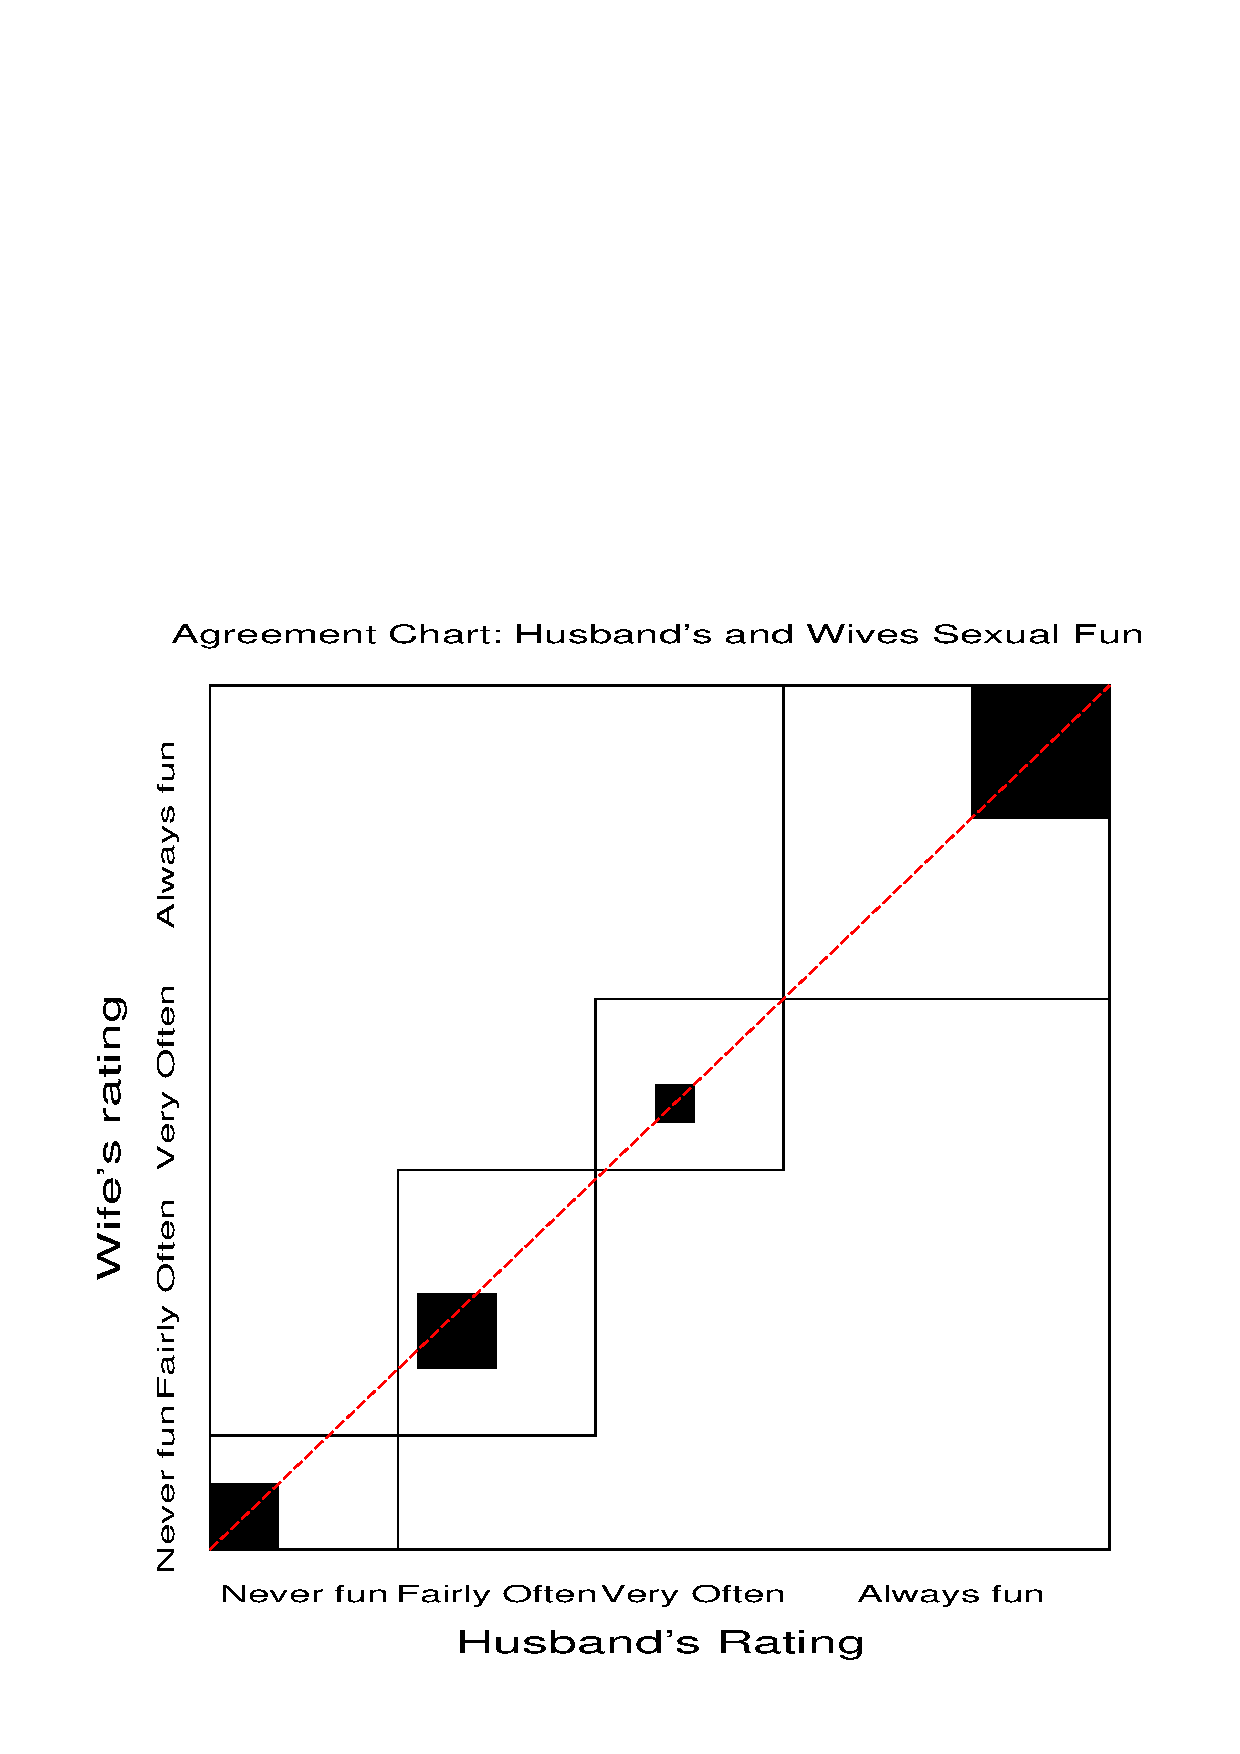
\includegraphics[width=1\linewidth,clip]{fig/agreemt1}
 \end{minipage}
 \hfill
 \begin{minipage}[c]{.33\textwidth}
  \includegraphics[width=1\linewidth,clip]{fig/mosaic3m1}
 \end{minipage}

Topics:
  \begin{itemize*}
    \item $2 \times 2$ tables and fourfold displays
	\item Sieve diagrams
	\item Observer agreement
%	\item Mosaic displays and \loglin\ models for \nway\ tables
	\item Correspondence analysis
  \end{itemize*}
\end{frame}


\renewcommand{\FileName}{vismethods}
\begin{frame}
%\makeatletter\slidebox@restore\makeatother
 
\frametitle{Visualizing contingency tables: software tools}
\begin{itemize}
\item Two-way tables
\begin{itemize*}
\item $2 \times 2$ ($\times k$) tables --- Visualize odds ratio (\macro{FFOLD})
%\item $2 \times 2 \times k$ tables --- Homogeneity of association
\item $r \times 3$ tables --- Trilinear plots (\macro{TRIPLOT})
\item $r \times c$ tables --- Visualize association (\macro{SIEVEPLOT})
\item $r \times c$ tables --- Visualize association (\macro{MOSAIC})
\item Square $r \times r$ tables --- Visualize agreement (\macro{AGREEPLOT})
\end{itemize*}
 
\item \nway\ tables
\begin{itemize*}
\item Fit \loglin\ models, visualize lack-of-fit --- (\macro{MOSAIC})
\item Test \& visualize partial association  --- (\macro{MOSAIC})
\item Visualize pairwise association  --- (\macro{MOSMAT})
\item Visualize conditional association  --- (\macro{MOSMAT})
\item Visualize \loglin\ structure  --- (\macro{MOSMAT})
\end{itemize*}
 
\item Correspondence analysis and MCA --- (\macro{CORRESP})
\item R: most of these in the \pkg{vcd} 
\begin{itemize*}
    \item \func{fourfold}, \func{sieve}, \func{mosaic}, \func{agreementplot}, $\dots$ --- more general
    \item Correspondence analysis: \pkg{ca}
\end{itemize*}

\end{itemize}
\end{frame}
 

\section{2 x 2 tables}
\renewcommand{\FileName}{twobytwo}

\begin{frame}
%\makeatletter\slidebox@restore\makeatother
\frametitle{Graphical Methods for 2$\times$2 tables: Example}
\begin{itemize}
 \item \citet{Bickel-etal:75}: data on admissions to graduate departments
 at Berkeley in 1973.
 \item Aggregate data for the six largest departments:
 \begin{table}[htb]
\caption{Admissions to Berkeley graduate programs}
\label{tab:berk22}
 \begin{center}
\begin{tabular}{lrr|rrr}
\hline
  & Admitted & Rejected & Total & \red{\% Admit} & \red{Odds(Admit)}\\
\hline
 Males & 1198 & 1493 & 2691  & \red{44.52} & \red{0.802}\\
 Females & 557 & 1278 & 1835 & \red{30.35} & \red{0.437}\\
\hline
 Total & 1755 & 2771 & 4526  & 38.78 & 0.633\\
\hline
\end{tabular}
\end{center}
\end{table}


 \item Evidence for gender bias?
 \begin{itemize}

 \item Odds ratio, 
 $\theta = \frac{\mbox{Odds}(\mbox{Admit}\given\mbox{Male})}{\mbox{Odds}(\mbox{Admit}\given\mbox{Female})} = 
 \frac{1198 / 1493}{557 / 1276} = \frac{0.802}{0.437} = 
 1.84$
 \item $\rightarrow$ Males 84\% more likely to be admitted. 
 \item Chi-square tests: $G^2_{(1)} = 93.7$, $\chi^2_{(1)} = 92.2, \: p < 0.0001$
 \end{itemize}
\end{itemize}

\end{frame}
\begin{frame}[plain]
\begin{center}
\includegraphics[width=.7\textwidth]{fig/Admissions2}
\end{center}
\begin{itemize*}
 \item How to analyse these data?
 \item How to visualize \& interpret the results?
 \item Does it matter that we collapsed over Department?
\end{itemize*}


\end{frame}

\subsection{Standard analysis}
\begin{frame}[fragile]
% \makeatletter\slidebox@restore\makeatother
 \frametitle{Standard analysis: PROC FREQ}

% \vspace{2ex}
\begin{Input}
 proc freq data=berkeley;
   weight freq;
   tables gender*admit / chisq;
\end{Input}
 Output:
\begin{Output}[gobble=7,baselinestretch=.8]
               Statistics for Table of gender by admit

       Statistic                     DF       Value      Prob
       ------------------------------------------------------
       Chi-Square                     1     92.2053    <.0001
       Likelihood Ratio Chi-Square    1     93.4494    <.0001
       Continuity Adj. Chi-Square     1     91.6096    <.0001
       Mantel-Haenszel Chi-Square     1     92.1849    <.0001
       Phi Coefficient                       0.1427          
\end{Output}
 How to visualize and interpret?
\end{frame}

\subsection{Fourfold displays}
\begin{frame}
% \makeatletter\slidebox@restore\makeatother
 \frametitle{Fourfold displays for 2 $\times$ 2 tables}
 \begin{itemize*}
 \item \boldital{Quarter circles}: radius $\sim \sqrt{n_{ij}} \Rightarrow$
 \textbf{area} $\sim$ \textbf{frequency}
 \item \boldital{Independence}: Adjoining quadrants $\approx$ align
 \item \boldital{Odds ratio}: ratio of areas of diagonally opposite cells
 \item \boldital{Confidence rings}: Visual test of 
 $H_0 : \theta = 1 \leftrightarrow$ \alert{adjoining rings overlap}

 \begin{center}
   \includegraphics[width=.45\dispwidth,clip]{fig/pie2x2g}
 \end{center}
 \item Confidence rings do not overlap: $\theta \neq 1$  (reject $H_0$)
 \end{itemize*}
\end{frame}

\begin{frame}
 %\makeatletter\slidebox@restore\makeatother
 \frametitle{Fourfold displays for 2 $\times$ 2 $\times $ \textit{k} tables}
 \begin{itemize*}
 \item Data in \tabref{tab:berk22} had been pooled over departments
 \item Stratified analysis: one fourfold display for each department
 \item Each $2 \times 2$ table standardized to equate marginal frequencies
 \item Shading: highlight departments for which $H_a : \theta_i \ne 1$

 \begin{center}
 %  \includegraphics[width=.6\dispwidth,clip]{fig/pie2x2bb.eps}
   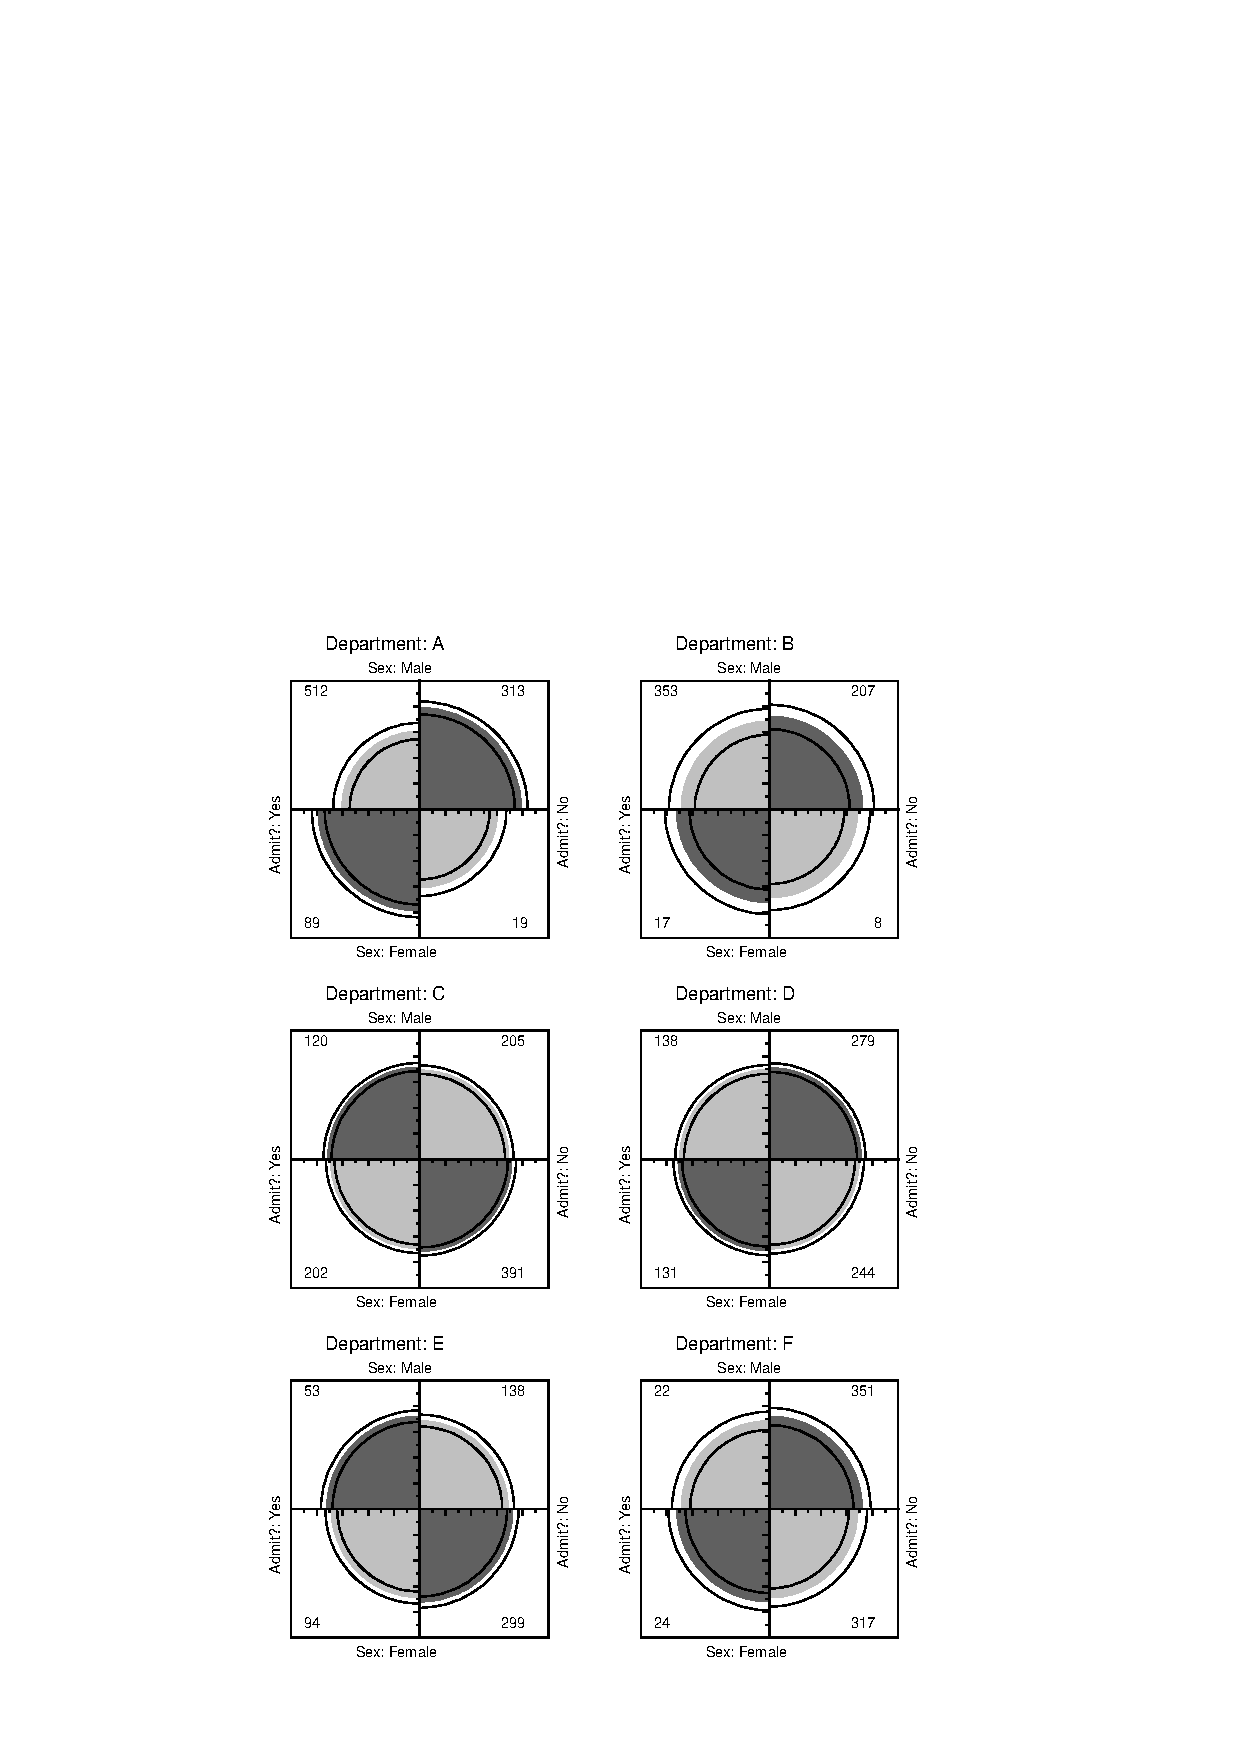
\includegraphics[width=.6\dispwidth,clip]{fig/pie2x2b}
 \end{center}
 \item Only one department (A) shows association; $\theta_A = 0.349 \rightarrow
 $ women $(0.349)^{-1} = 2.86$ times as likely as men to be admitted.
 \end{itemize*}
 \end{frame}

\begin{frame}
 %\makeatletter\slidebox@restore\makeatother
   \frametitle{What happened here?}
  Why do the results \emph{collapsed over} department disagree with the results \emph{by} department?
  \begin{block}{Simpson's paradox}
   \begin{itemize}
	 \item<1-> Aggregate data are misleading because they falsely
	 assume men and women apply \emph{equally} in each field.
	 \item<2-> But:
	   \begin{itemize*}
	   \item Large differences in admission rates across departments.
	   \item Men and women apply to these departments differentially.
	   \item Women applied in large numbers to departments with low admission rates.
	 \end{itemize*}
	 \item<3->
	  Other graphical methods can show these effects.
 	 \item<3-> (This ignores possibility of \emph{structural bias} against women:
	 differential funding of fields to which women are more likely to apply.)
  \end{itemize}
  \end{block}
\end{frame}

\begin{frame}[fragile]
%\makeatletter\slidebox@restore\makeatother

\frametitle{The \sasprogt{FOURFOLD} and the \macrot{FFOLD}}
  \begin{itemize*}
  \item The \sasprog{FOURFOLD} is written in \IML.
  \item The \macro{FFOLD} provides a simpler interface.
  \item Printed output: (a) significance tests for individual odds ratios,
  (b) tests of homogeneity of association (here, over departments) and
  (c) conditional association (controlling for department).
  \end{itemize*}
Plot by department:
\begin{Input}[fontsize=\small,label=\fbox{\texttt{berk4f.sas}},baselinestretch=0.8]
%include catdata(berkeley);

%ffold(data=berkeley, 
   var=Admit Gender,       \sascomment{/* panel variables   */} 
   \sasemph{by=Dept},                \sascomment{/* stratify by dept  */}
   down=2, across=3,       \sascomment{/* panel arrangement */}
   htext=2);               \sascomment{/* font size         */}
\end{Input}
Aggregate data: first sum over departments,
using the \macro{TABLE}:
\begin{Input}[fontsize=\small,baselinestretch=0.9,firstnumber=8]
%table(data=berkeley, \sasemph{out=berk2}, 
   var=Admit Gender,       \sascomment{/* omit dept          */}
   weight=count,           \sascomment{/* frequency variable */}
   order=data);
%ffold(\sasemph{data=berk2}, var=Admit Gender);
\end{Input}
\end{frame}

\subsection{Odds ratio plots}
\begin{frame}[fragile]
\frametitle{Odds ratio plots}
\begin{Rin}
> library(vcd)
> oddsratio(UCBAdmissions, log=FALSE)
\end{Rin}
\begin{Rout}
    A     B     C     D     E     F 
0.349 0.803 1.133 0.921 1.222 0.828 
\end{Rout}
\begin{Rin}
> lor <- oddsratio(UCBAdmissions)  # capture log odds ratios
> plot(lor)
\end{Rin}
\begin{center}
   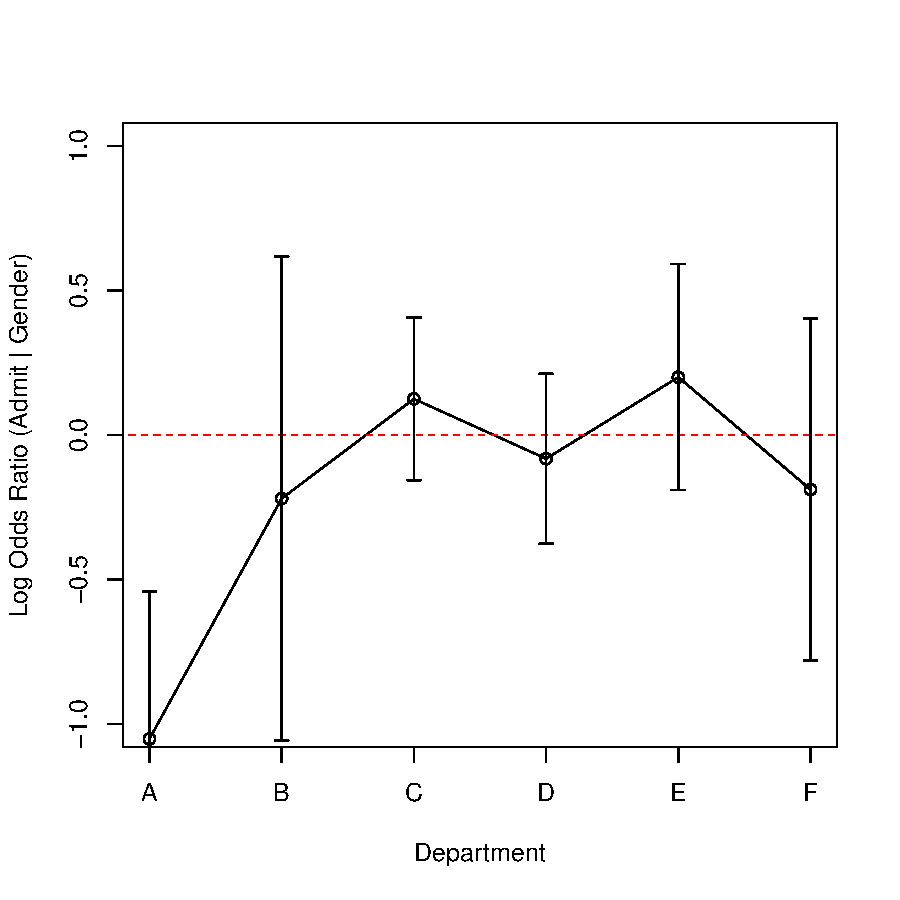
\includegraphics[width=.45\dispwidth,clip,trim=0 20 20 40]{fig/vcd-tut-oddsratio}
\end{center}

\end{frame}

\section{Two-way tables}
\section{Two-way tables}\label{sec:mosaic-twoway}
The mosaic display 
\citep{Friendly:92b,Friendly:94a,Friendly:97,HartiganKleiner:81,HartiganKleiner:84}
is like a grouped barchart,
where the widths of the bars show the relative frequencies of one
variable, and heights of the sections in each bar show the
relative frequencies of the second variable as shown in \figref{fig:mosaic31}.
% Additional variables can be displayed by dividing 
The construction of the mosaic display, and what it reveals,
are most easily understood for two-way tables.

\begin{Example}[haireye2a]{Hair color and eye color}
Consider the data in \tabref{tab:hairdat},
showing the relation between hair color and eye color among students
in a statistics course.
\begin{figure}[htb]
  \centering
  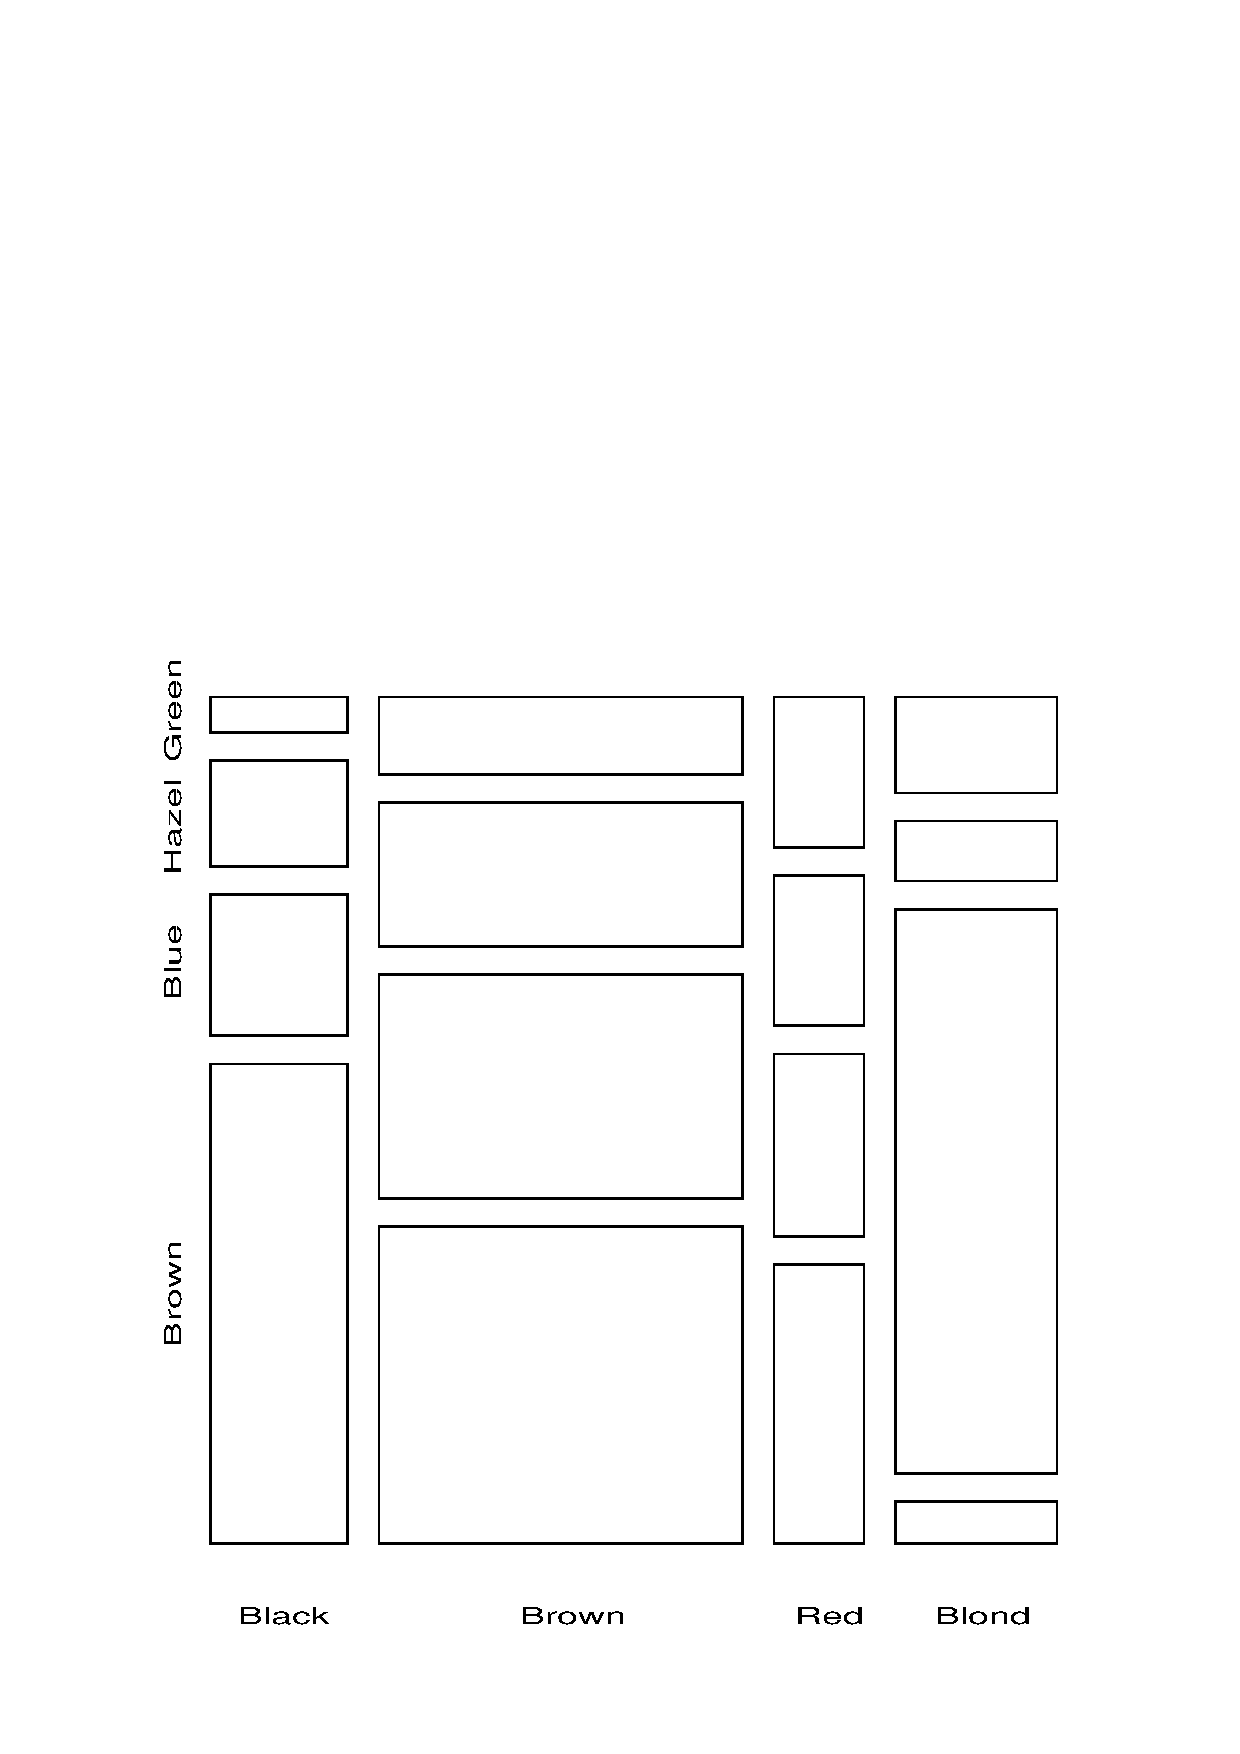
\includegraphics[scale=.6]{ch4/fig/mosaic31}
  \caption[Basic mosaic display for hair color and eye color data]{Basic mosaic display for hair color and eye color data.  The area of each
  rectangle is proportional to the observed frequency in that cell.}%
  \label{fig:mosaic31}
\end{figure}
For such a two-way table, the mosaic display is constructed
by first dividing a unit square in proportion to the marginal
totals of one variable, say, Hair color.

For these data, the marginal frequencies and proportions are:

\begin{minipage}{\linewidth} 
\begin{verbatim} 
              Black      Brown      Red    Blond    TOTAL
Frequencies    108       286        71      127      592
Proportions   0.1824    0.4831    0.1199   0.2145   1.000
\end{verbatim}
\end{minipage}


These can be shown as the mosaic for the first variable (hair color),
as in \figref{fig:mosaic32}.
The rectangular tiles are shaded to show the residuals (deviations)
from a particular model, as follows:
\begin{figure}[htb]
  \centering
  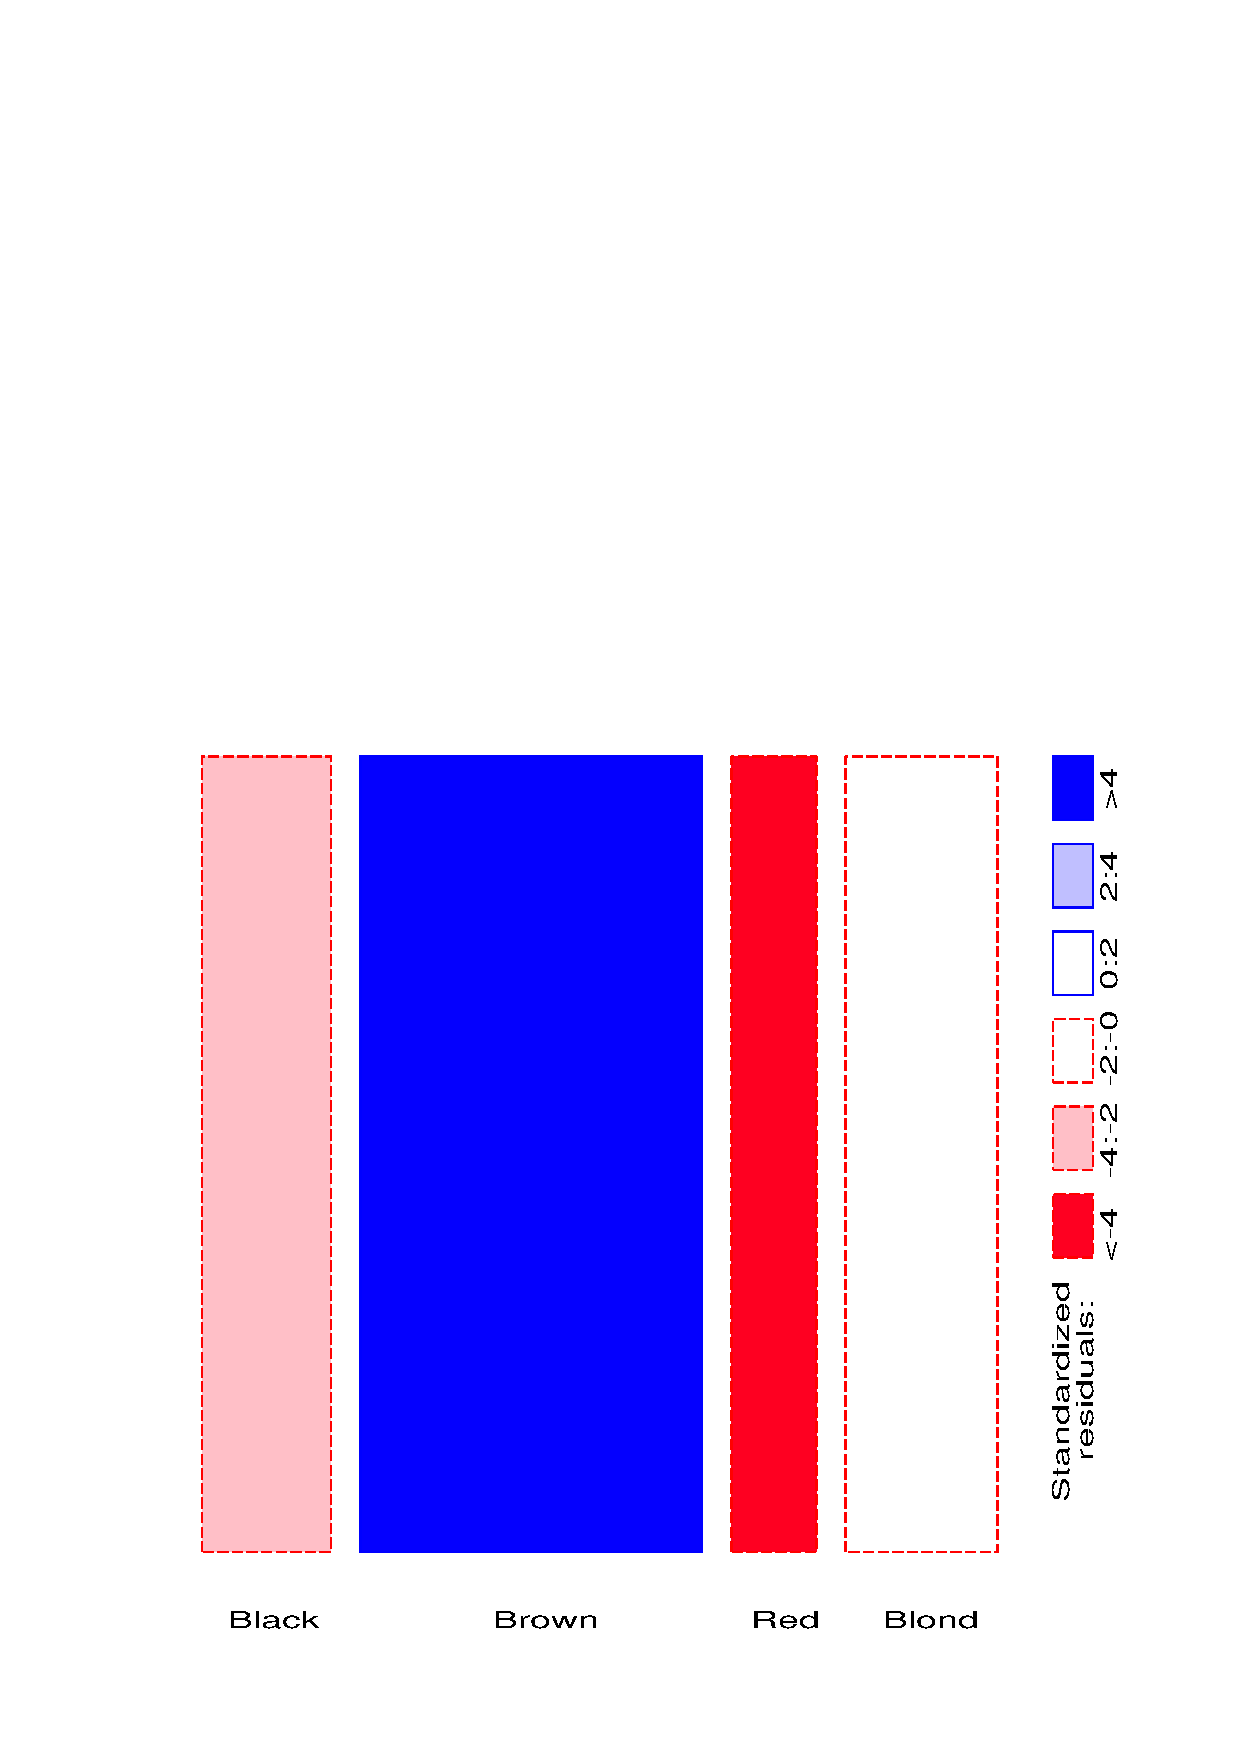
\includegraphics[scale=.6]{ch4/fig/mosaic32}
  \caption{First step in the mosaic display}%
  \label{fig:mosaic32}
\end{figure}

\begin{itemize}
\item The one-way table of marginal totals can be fit to a model, in this
case, the model that all hair colors are equally probable.  This model
has expected frequencies $m_i = 592/4$:
\begin{verbatim} 
               Fitted frequencies
       Black      Brown      Red    Blond
       148.00    148.00    148.00   148.00
\end{verbatim}
\item The Pearson residuals from this model, $d_i = ( n_i - m_i ) / \sqrt{m_i}$, are:
\begin{verbatim} 
         Standardized Pearson residuals
       Black    Brown      Red    Blond
       -3.29    11.34    -6.33    -1.73
\end{verbatim}
and these values are shown by color and shading as shown in the legend.
The high positive value for Brown hair indicates that people
with brown hair are much more frequent in this sample than 
the Equiprobability model would predict.
\end{itemize}

Next, the rectangle for each Hair color is subdivided in proportion
to the relative (conditional) frequencies of the second variable --
Eye color, giving the following conditional proportions:
\begin{verbatim} 
                     Marginal proportions
                Brown     Blue    Hazel    Green   TOTAL

      Black    0.6296   0.1852   0.1389   0.0463    1.0
      Brown    0.4161   0.2937   0.1888   0.1014    1.0
      Red      0.3662   0.2394   0.1972   0.1972    1.0
      Blond    0.0551   0.7402   0.0787   0.1260    1.0
\end{verbatim}
The proportions in each row determine the heights of the tiles in the second mosaic display in \figref{fig:mosaic33}.
\begin{figure}[htb]
  \centering
  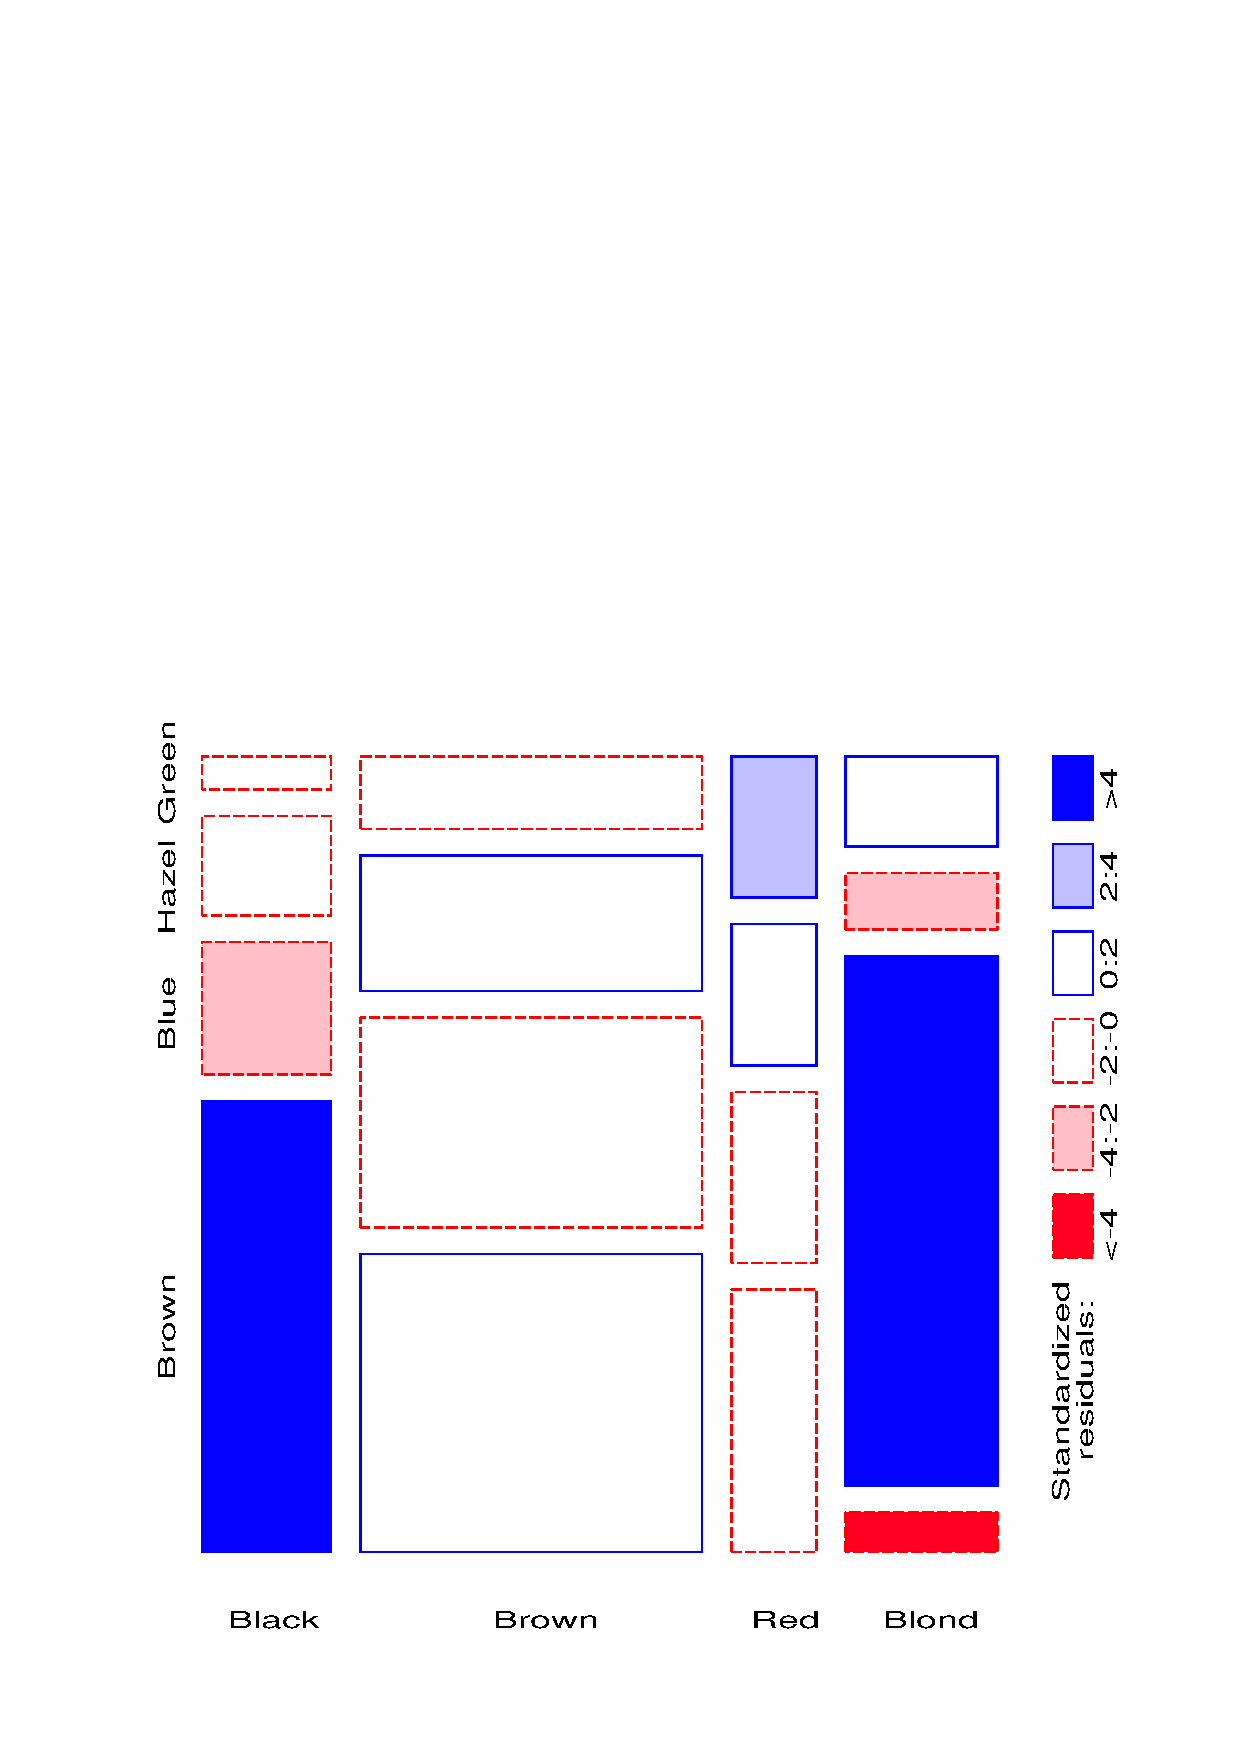
\includegraphics[scale=.6]{ch4/fig/mosaic33}
  \caption[Second step in the mosaic display]{Second step in the mosaic display.  Each rectangle for hair color is subdivided in proportion to the
  frequencies of eye color.}%
  \label{fig:mosaic33}
\end{figure}

\begin{itemize}
\item Again, the cells are shaded in relation to standardized
residuals, \(d_{ij} = (
n_{ij} - m_{ij}) / \sqrt { m_{ij} }\), 
from a model.  For a two-way table, the model is that Hair color and
Eye color are independent in the population from which this sample
was drawn.
\begin{verbatim} 
               Standardized Pearson residuals
               Brown     Blue    Hazel    Green

      Black     4.40    -3.07    -0.48    -1.95
      Brown     1.23    -1.95     1.35    -0.35
      Red      -0.07    -1.73     0.85     2.28
      Blond    -5.85     7.05    -2.23     0.61
\end{verbatim}
\item Thus, the two tiles shaded deep blue correspond to the two
cells, (Black, Brown) and (Blond, Blue), whose residuals are
greater than $+4$, indicating much greater frequency in those
cells than would be found if Hair color and Eye color were
independent.
The tile shaded deep red, (Blond, Brown)
corresponds to the largest residual = -5.85, indicating this combination
is extremely rare under the hypothesis of independence.
\item The overall Pearson \chisq{} statistic is just the
sum of squares of the residuals.
\end{itemize}
\end{Example}

\subsubsection{Shading levels}

The default shading patterns for the tiles are based on standardized
residuals which exceed the values 2 and 4 in absolute value.%
\footnote{In \Dset{}s with very large total frequency,
most models may fit poorly and have large residuals.
In such cases (e.g., \exref{ex:suicide1}) it is often useful to define
more shading levels to make finer distinctions.  For example,
in \exref{ex:suicide1} we use \pname{SHADE=\{2 4 8\};} to set
three levels of shading.}
Since the standardized residuals are approximately unit-normal $N(0,1)$
values,  this corresponds to highlighting cells whose
residuals are \emph{individually} significant at approximately
the .05 and .0001 level, respectively.
The purpose of highlighting cells, however, is not to provide tests
of significance, but rather to draw attention to the \emph{pattern}
of departures of the data from the assumed model.
In any case, 
the number and values of
these cutoffs can be easily set by the user using the \pname{SHADE}
parameter.

To provide some redundancy when color figures are reproduced in 
black and white, cells with positive residuals are outline with solid
(blue) lines, while cells with negative residuals are outlined with broken
(red) lines.
Cells whose absolute residuals are less than the smallest shading level
are unfilled.  For good-fitting models, it is sometimes useful to distinguish
between near-zero residuals and small, non-significant residuals.
In color figures, near-zero cells are outlined in solid black;
the threshold is determined by the \pname{FUZZ} parameter.

\subsubsection{Interpretation}

To interpret the association between Hair color and Eye color,
consider the pattern of positive (Blue) and negative (Red)
tiles in the mosaic display.  
We interpret positive values as showing cells whose observed frequency
is substantially greater than would be found under independence;
negative values indicate cells which occur less often than
under independence.

\ixe{Hair color and eye color|(}
This interpretation is enhanced by reordering the rows or columns
of the two-way table so that the residuals have an opposite
corner pattern of signs.  This usually helps us interpret any systematic
patterns of association in terms of the ordering of the row and column
categories.
Here, this is achieved by reordering the Eye colors as shown in
\figref{fig:mosaic34},  and we note that in this rearrangement
both hair colors and eye colors are ordered from dark to light.
(In general, the levels of a factor may be reordered by
arranging them according to their scores on the first (largest)
correspondence analysis dimension; see
\citep{Friendly:94a}).
The re-ordered residuals are:
\begin{verbatim} 
         Standardized Pearson residuals

          Brown    Hazel    Green     Blue

Black      4.40    -0.48    -1.95    -3.07
Brown      1.23     1.35    -0.35    -1.95
Red       -0.07     0.85     2.28    -1.73
Blond     -5.85    -2.23     0.61     7.05
\end{verbatim}
\begin{figure}[htb]
  \centering
  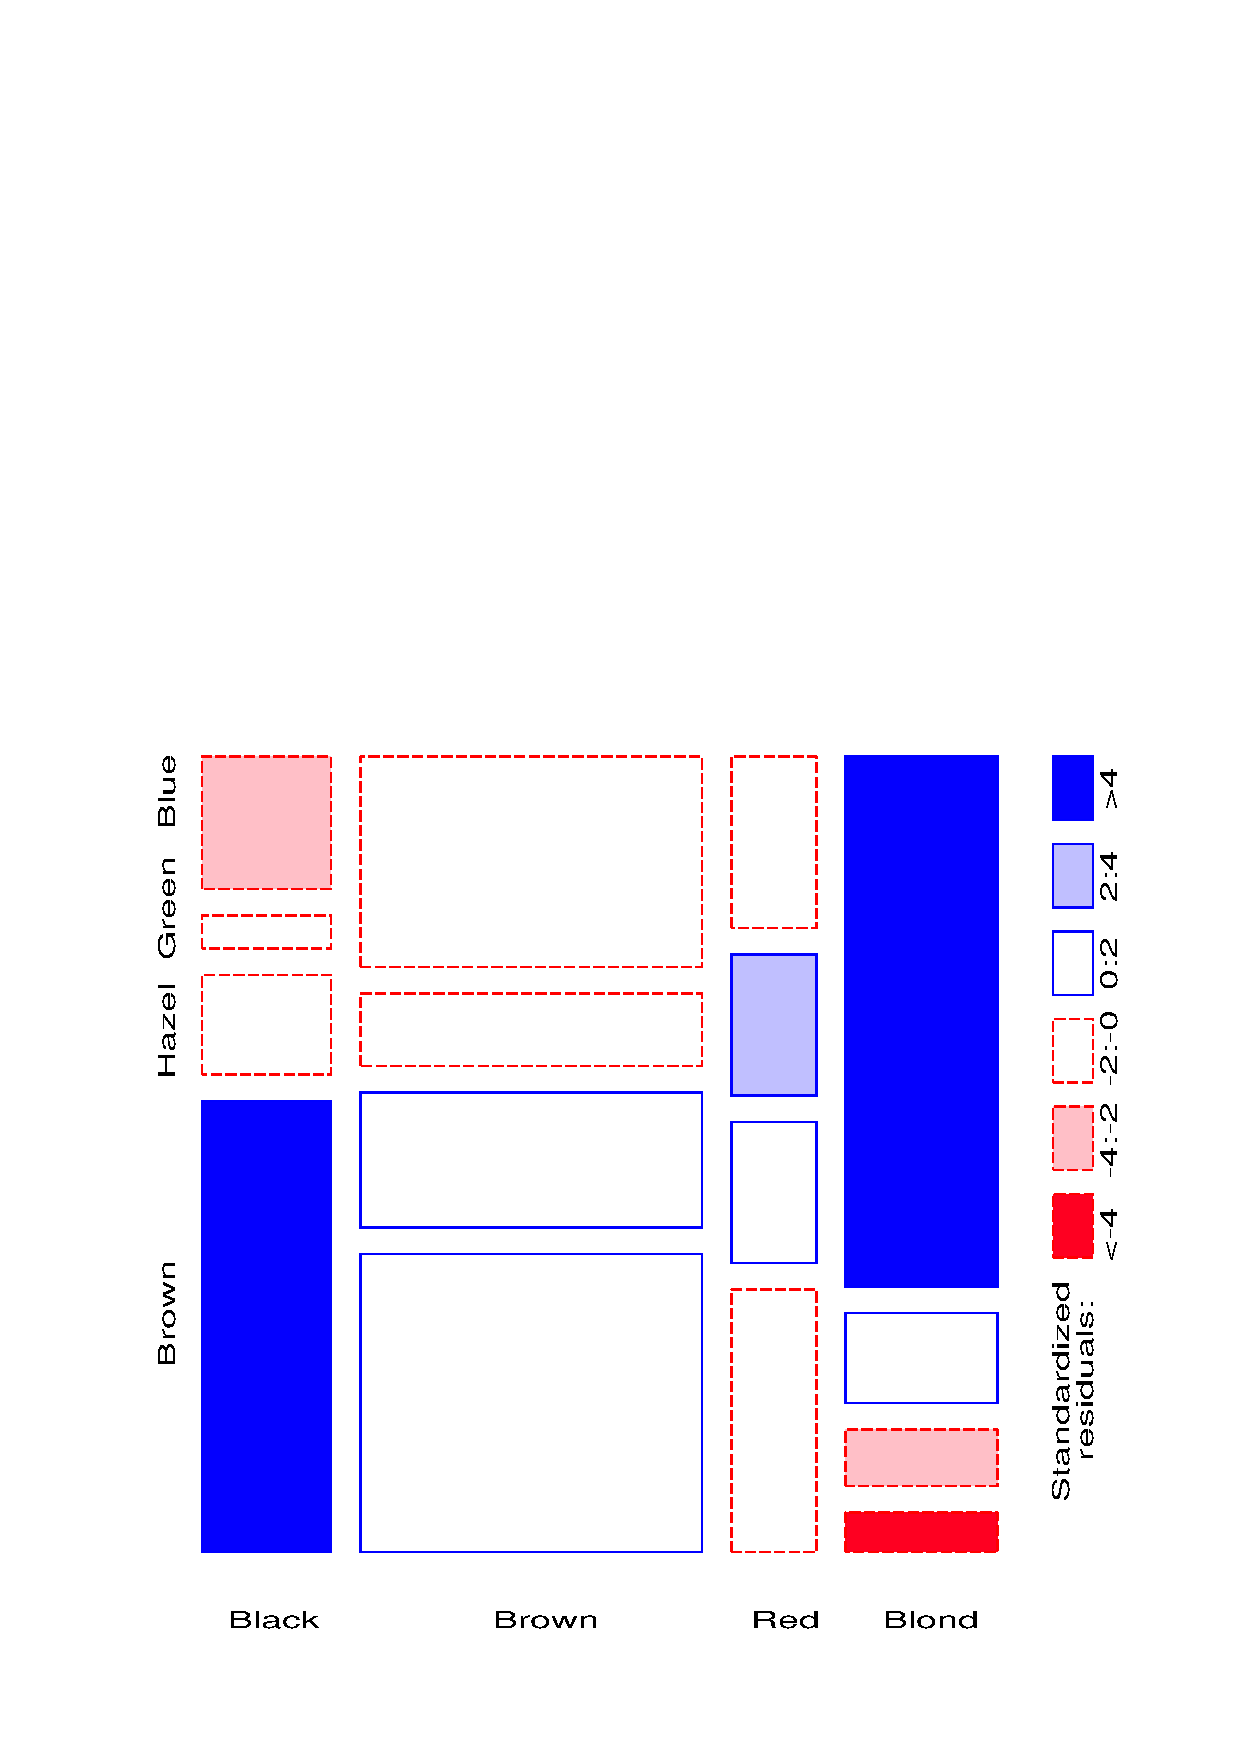
\includegraphics[scale=.6]{ch4/fig/mosaic34}
  \caption[Two-way mosaic, reordered]{Two-way mosaic,
  reordered.  Deviations from independence are shown by
  color and shading.  The two levels of shading density correspond to
  standardized deviations greater than 2 and 4 in absolute value.
  This form of the display generalizes readily to multi-way
  tables.}  \label{fig:mosaic34}
\end{figure}
Thus, the mosaic shows that the association between Hair and Eye color
is essentially that 
\begin{itemize*}
\item people with dark hair tend to have dark eyes,
\item those with light hair tend to have light eyes
\item people with red hair do not quite fit this pattern
\end{itemize*}
\ixe{Hair color and eye color|)}

\subsection{Software for mosaic displays}
Mosaic displays are implemented as a collection of modules
(the \sasprog{mosaics.sas}) written in \IML{},
which are used within a \PROC{IML} step,
as described in \macref{mac:mosaics}.  The program is designed so that
the frequency table, and its associated factor levels and variable names
may be entered directly using \IML{} statements,
or (using the \module{readtab}) may be input from a SAS \Dset\
of the form produced by \PROC{FREQ}.
Using the \sasprog{mosaics.sas} within a \PROC{IML} step is most
flexible, because you can use \IML{} statements and modules within
\texttt{mosaics.sas} to manipulate the frequency table (selecting
or reordering rows or columns), to specify structural zeros,
or to fit specialized models which cannot be fit by other means.

In addition, several SAS macros
are provided to simplify the use of \texttt{mosaics.sas}. 
The \macro{MOSAIC} (described in \macref{mac:mosaic})
may be used with any SAS \Dset\ in frequency
form (e.g., the output from \PROC{FREQ}).  It reads the data into
\IML{} and provides basic mosaic displays,
mosaics for externally-calculated residuals,
and partial mosaic displays (\secref{sec:mospart}).
The \macro{TABLE} (\macref{mac:table}) may be used to construct the frequency table, and
to collapse or recode variables.
The \macro{MOSMAT} (\macref{mac:mosmat})
provides mosaic matrices (\secref{sec:mosmat}),
an analog of the \scatmat{} for categorical data.

Two examples below illustrate the use of this software for basic mosaic
displays.
\exref{ex:soccer2} uses the \macro{MOSAIC},
while \exref{ex:victims}
uses \PROC{IML} statements to construct and manipulate the
frequency table.

\begin{table}[!hb]
\caption{Total goals scored in 380 games in the Premier
Football League, 1995/95 season}
\label{tab:soccer2}
\vspace{.1in}
\begin{center}
\begin{tabular}{l|rrrr rrrr}
\hline
Total goals      &  0  &  1  &  2  &  3  &  4  &  5  &  6  &  7  \\
\hline
Number of games  & 27  & 88  & 91  & 73  & 49  & 31  & 18  &  3  \\
  \hline
\end{tabular}
\end{center}
\end{table}

%%
% Table victims written by md2tex  1-29-1998
\begin{table}[htb]
 \caption{Repeat Victimization Data}
 \label{tab:victims}
 \begin{center}
  \begin{tabular}{|l|rrrrrrrr|}
   \hline
 & \multicolumn{8}{c|}{\bfseries\large First Victimization }\rule{0in}{2.5ex}\\
{\bfseries\large Second       } &          &       &       & Pick     & Personal &      & Household & Auto    \\
{\bfseries\large Victimization} & Rape     & Assault & Robbery & Pocket & Larceny & Burglary & Larceny & Theft   \\
   \hline
% f=        2 t=        1
Rape                   &            26 &            65 &            12 &             3 &            75 &            52 &            42 &             3 \\
Assault                &            50 &          2997 &           279 &           102 &          2628 &          1117 &          1251 &           221 \\
Robbery                &            11 &           238 &           197 &            40 &           413 &           191 &           206 &            51 \\
Pick Pocket            &             6 &            85 &            36 &            61 &           329 &           102 &           117 &            24 \\
Personal Larceny           &            82 &          2553 &           459 &           243 &         12137 &          2649 &          3757 &           678 \\
Burglary               &            39 &          1083 &           197 &           115 &          2658 &          3210 &          1962 &           301 \\
Household Larceny           &            48 &          1349 &           221 &           101 &          3689 &          1973 &          4646 &           367 \\
Auto Theft             &            11 &           216 &            47 &            38 &           687 &           301 &           391 &           269 \\
   \hline
  \end{tabular}
 \end{center}
\end{table}


\section{Observer Agreement}
\renewcommand{\FileName}{agree}
% slide template
\begin{frame}
  \frametitle{Observer Agreement}
  \begin{itemize}
	\item {\large\bfseries Inter-observer agreement} often used as to assess 
reliability of a subjective classification or assessment procedure
      \begin{itemize*}
        \item $\rightarrow$ square table, Rater 1 x Rater 2
	    \item Levels: diagnostic categories (normal, mildly impaired, severely
		impaired)
	  \end{itemize*}
	\item{\large\bfseries Agreement vs.\ Association:} Ratings can be strongly associated 
	without strong agreement
	\item{\large\bfseries Marginal homogeneity:}  Different frequencies of
	category use by raters affects measures of agreement
	\item{\large\bfseries Measures of Agreement:}
      \begin{itemize*}
	  \item Intraclass correlation:  ANOVA framework--- multiple raters!
	  \item Cohen's $\kappa$: compares the observed agreement, \(P_o  =
\sum p_{ii}\), to agreement expected by chance if the two observer's
ratings were independent, \(P_c = \sum p_{i+} \,  p_{+i}\).
  \begin{equation*} \label{eq:kappa}
  \kappa =  \frac{ P_o - P_c } { 1 - P_c }
  \end{equation*}
      \end{itemize*}
  \end{itemize}
\end{frame}

\subsection[Cohen's kappa]{Cohen's kappa}
\begin{frame}[fragile]
  \frametitle{Cohen's $\kappa$}
  \begin{itemize*}
      \item Properties of Cohen's $\kappa$:
    	\begin{itemize*}
		\item perfect agreement: \(\kappa = 1\)
		\item minimum \(\kappa\) may be \(< 0\); lower bound depends on marginal
       totals
	    \item Unweighted $\kappa$: counts only diagonal cells (same
       category assigned by both observers).
	    \item Weighted $\kappa$: allows partial credit for near agreement.
		(Makes sense only when the categories are \emph{ordered}.)
		\end{itemize*}
	  \item Weights:  
    	\begin{itemize*}
			\item Cicchetti-Alison (inverse integer spacing) vs.\
	  		\item Fleiss-Cohen (inverse square spacing)
 		\end{itemize*}
 \end{itemize*}

\begin{Output}[fontsize=\footnotesize]
       Integer Weights                 Fleiss-Cohen Weights
   1     2/3     1/3       0          1     8/9     5/9      0
 2/3       1     2/3     1/3        8/9       1     8/9    5/9
 1/3     2/3       1     2/3        5/9     8/9       1    8/9
   0     1/3     2/3       1          0     5/9     8/9      1
\end{Output}

\end{frame}

\begin{frame}[fragile]
  \frametitle{Cohen's $\kappa$: Example}
The table below summarizes responses of 91
married couples to a questionnaire item,

\begin{quote}
Sex is fun for me and my partner (a) Never or occasionally, (b)
fairly often, (c) very often, (d) almost always.  
\end{quote}
\vspace{2em}

\begin{Output}
              --------- Wife's Rating --------
Husband's     Never   Fairly     Very   Almost
Rating          fun    often    Often   always    |   SUM    
--------------------------------------------------+-------
Never fun         \sasemph{7}        7        2        3    |    19
Fairly often      2        \sasemph{8}        3        7    |    20
Very often        1        5        \sasemph{4}        9    |    19
Almost always     2        8        9       \sasemph{14}    |    33
--------------------------------------------------+-------
SUM              12       28       18       33    |    91    
\end{Output}
\end{frame}

\begin{frame}[fragile]
  \frametitle{Computing $\kappa$ with SAS}
  \begin{itemize}
	\item \PROC{FREQ}: Use \texttt{AGREE} option on \texttt{TABLES} statement
      \begin{itemize*}
	  \item Gives both unweighted and weighted $\kappa$ (default: CA weights)
	  \item \texttt{AGREE (wt=FC)} uses Fleiss-Cohen weights
	  \item Bowker's \citep{Bowker:48} test of symmetry: $H_0 : p_{ij} = p_{ji}$
	  \end{itemize*}
  \end{itemize}

\vspace{2ex}
\begin{Input}[fontsize=\footnotesize,label=\fbox{\texttt{kappa3.sas}},baselinestretch=0.8]
title 'Kappa for Agreement';
data fun;
   do Husband = 1 to 4;
   do Wife    = 1 to 4;
      input count @@;
      output;
      end; end;
datalines;
 7     7     2      3
 2     8     3      7
 1     5     4      9
 2     8     9     14
;
proc freq;
  weight count;
  tables Husband * Wife / noprint \sasemph{agree};      \sascomment{/* default: CA weights*/}
  tables Husband * Wife / noprint \sasemph{agree(wt=FC)};
\end{Input}
\end{frame}

\begin{frame}[fragile]
  \frametitle{Computing $\kappa$ with SAS}
Output (CA weights):
\begin{Output}[baselinestretch=0.8,gobble=3]
              Statistics for Table of Husband by Wife

                         Test of Symmetry
                      -----------------------
                      Statistic (S)    3.8778
                      DF                    6
                      Pr > S           0.6932

                          Kappa Statistics
 
    Statistic          Value       ASE     95% Confidence Limits
    ------------------------------------------------------------
    Simple Kappa      0.1293    0.0686      -0.0051       0.2638
    Weighted Kappa    0.2374    0.0783       0.0839       0.3909

                          Sample Size = 91
\end{Output}
Using Fleiss-Cohen weights:
\begin{Output}[gobble=3]
    Weighted Kappa    0.3320    0.0973       0.1413       0.5227
\end{Output}
\end{frame}

\begin{frame}[fragile]
  \frametitle{Observer agreement: Multiple strata}
  \begin{itemize}
	\item When the individuals rated fall into multiple groups, one can test for:
      \begin{itemize*}
	  \item Agreement within each group
	  \item Overall agreement (controlling for group)
	  \item Homogeneity: Equal agreement across groups
      \end{itemize*}
  \end{itemize}
Example: Diagnostic classification of mulitiple sclerosis by two neurologists,
for two populations \citep{LandisKoch:77}
\begin{listing}[baselinestretch=0.8]
                 Winnipeg patients        New Orleans patients
  NO rater:
                Cert Prob  Pos Doubt      Cert Prob  Pos Doubt 
                --------------------      --------------------
Winnipeg rater:
 Certain MS      38    5    0    1          5    3    0    0
 Probable        33   11    3    0          3   11    4    0
 Possible        10   14    5    6          2   13    3    4
 Doubtful MS      3    7    3   10          1    2    4   14 
\end{listing}
Analysis:
\begin{Input}[numbers=none]
 proc freq;
   tables \sasemph{strata} * rater1 * rater2 / \sasemph{agree};
\end{Input}

\end{frame}

\begin{frame}[fragile]
  \frametitle{Observer agreement: Multiple strata}
\begin{Input}[fontsize=\footnotesize,label=\fbox{\texttt{msdiag.sas}},baselinestretch=0.8]
data msdiag;
  do patients='Winnipeg  ', 'New Orleans';
     do N_rating = 1 to 4;
        do W_rating = 1 to 4;
           input count @;
           output;
           end;
        end;
     end;
 label N_rating = 'New Orleans neurologist'
       W_rating = 'Winnipeg neurologist';
datalines;
38  5  0  1
33 11  3  0
10 14  5  6
 3  7  3 10
 5  3  0  0
 3 11  4  0
 2 13  3  4
 1  2  4 14
;

*-- Agreement, separately, and controlling for Patients;
proc freq data=msdiag;
   weight count;
   tables \sasemph{patients} * N_rating * W_rating / norow nocol nopct agree;
\end{Input}
\end{frame}

\begin{frame}[fragile]
  \frametitle{Observer agreement: Multiple strata}
Output, strata 1: (New Orleans patients):
\begin{Output}[baselinestretch=0.8,gobble=3]
           Statistics for Table 1 of N_rating by W_rating
                Controlling for patients=New Orleans

                         Test of Symmetry
                      -----------------------
                      Statistic (S)    9.7647
                      DF                    6
                      Pr > S           0.1349

                          Kappa Statistics
 
    Statistic          Value       ASE     95% Confidence Limits
    ------------------------------------------------------------
    Simple Kappa      0.2965    0.0785       0.1427       0.4504
    Weighted Kappa    0.4773    0.0730       0.3341       0.6204

                          Sample Size = 69
\end{Output}
\end{frame}

\begin{frame}[fragile]
  \frametitle{Observer agreement: Multiple strata}

Output, strata 2: (Winnipeg patients):
\begin{Output}[baselinestretch=0.8,gobble=3]
           Statistics for Table 2 of N_rating by W_rating
                 Controlling for patients=Winnipeg

                          Test of Symmetry
                      ------------------------
                      Statistic (S)    46.7492
                      DF                     6
                      Pr > S            <.0001

                          Kappa Statistics
 
    Statistic          Value       ASE     95\% Confidence Limits
    ------------------------------------------------------------
    Simple Kappa      0.2079    0.0505       0.1091       0.3068
    Weighted Kappa    0.3797    0.0517       0.2785       0.4810

                         Sample Size = 149
\end{Output}
\end{frame}

\begin{frame}[fragile]
  \frametitle{Observer agreement: Multiple strata}

Overall test:
\begin{Output}[baselinestretch=0.8,gobble=3]
            Summary Statistics for N_rating by W_rating
                      \sasemph{Controlling for patients}

                     Overall Kappa Coefficients
 
    Statistic          Value       ASE     95\% Confidence Limits
    ------------------------------------------------------------
    Simple Kappa      0.2338    0.0424       0.1506       0.3170
    Weighted Kappa    0.4123    0.0422       0.3296       0.4949
\end{Output}
Homogeneity test:  $H_0: \kappa_1 = \kappa_2 = \dots = \kappa_k$
\begin{Output}[baselinestretch=0.8]
                \sasemph{Tests for Equal Kappa Coefficients}
 
          Statistic         Chi-Square    DF    Pr > ChiSq
          ------------------------------------------------
          Simple Kappa          0.9009     1      0.3425  
          Weighted Kappa        1.1889     1      0.2756  

                      Total Sample Size = 218
\end{Output}
\end{frame}

\begin{frame}
 \frametitle{Observer agreement: SAS 9.3 ODS graphs}
% three figures in tabular layout
 \begin{minipage}[c]{.5\linewidth}
  \centering
  \includegraphics[width=.95\linewidth]{fig/msdiag-WtKappaPlot}
    \\ \texttt{agree} option $\rightarrow$ plots of CIs for $\kappa$ ... 
 \end{minipage}%
 \begin{minipage}[c]{.5\linewidth}
  \centering
  \begin{tabular}{c}
  \includegraphics[width=.8\linewidth]{fig/msdiag-AgreePlot1} \\
  \includegraphics[width=.8\linewidth]{fig/msdiag-AgreePlot2} \\
   ... and agreement plots (next)
  \end{tabular}
 \end{minipage}
\end{frame}



\subsection{Observer Agreement Chart}
\begin{frame}
  \frametitle{Bangdiwala's Observer Agreement Chart}
  \begin{itemize}
	\item The observer agreement chart \cite{Bangdiwala:87} provides
      \begin{itemize*}
	  \item a simple graphic representation of the strength of agreement, and 
 	  \item a measure of strength of agreement with an intuitive
interpretation.
	  \end{itemize*}
	 

	\item Construction: 
      \begin{itemize*}
	  \item \(n \times  n\) square, $n$=total sample size
	  \item Black squares, each of size \(n_{ii} \times  n_{ii} \rightarrow\)  observed agreement
	  \item Positioned within larger rectangles, each of size \(n_{i+} \times  n_{+i} \rightarrow\) maximum possible agreement
	  \item $\Rightarrow$ visual impression of the strength of agreement is
	  \end{itemize*}
  \begin{equation*}
  B_N  =
  \frac{ \mbox{area of dark squares}}
  { \mbox{area of rectangles}}  =
  \frac{ \sum_i^k \,  n_{ii}^2 }
  { \sum_i^k \,  n_{i+} \,  n_{+i} }
  \end{equation*}
  \end{itemize}
\end{frame}

\begin{frame}
Husbands and wives: $B_N = .146$
 \begin{center}
 \includegraphics[width=.7\textwidth,clip,keepaspectratio]{fig/agreemt1}
 \end{center}
  
\end{frame}

\begin{frame}
  \frametitle{Weighted Agreement Chart: Partial agreement}
 Partial agreement:
include  weighted contribution from off-diagonal cells, \(b\)
steps from the main diagonal, using weights $ 1 > w_1 > w_2 > \cdots$.

  \[
 \left.
 \begin{array}{ccccc}
   &  & n_{i-b,i} &  & \\
    &  & \vdots    &  & \\
    n_{i, i-b} & \cdots & n_{i, i} & \cdots & n_{i, i+b} \\
    &  & \vdots    &  & \\
   &  & n_{i-b,i} &  &
 \end{array}
  \right.
  \qquad
 \left.
 \begin{array}{ccccc}
   &  & w_2 &  & \\
   &  & w_1 &  & \\
 w_2 & w_1 & 1 & w_1 & w_2 \\
   &  & w_1 &  & \\
   &  & w_2 &  & \\
 \end{array}
  \right.
  \]

  \begin{itemize}
	\item Add shaded rectangles, size $\sim$ sum of frequencies, \(A_{bi}\), within $b$ steps of main diagonal
	\item $\Rightarrow$ weighted measure of agreement,
  \[
  B_N^w  =
  \frac{ \mbox{weighted sum  of agreement}}
  { \mbox{area of rectangles} }  =
  1 - \frac{ \sum_i^k \,
  [ n_{i+} n_{+i} - n_{ii}^2  -
  \sum_{b=1}^q \,  w_b  A_{bi} ] }
  { \sum_i^k \,  n_{i+} \,  n_{+i} }
  \]
  \end{itemize}
\end{frame}

\begin{frame}
Husbands and wives: $B_N^w = .628$ with $w_1 = 8/9$
 \begin{center}
 \includegraphics[width=.7\textwidth,clip,keepaspectratio]{fig/agreemt2}
 \end{center}
\end{frame}

\renewcommand{\FileName}{agree-Sex-SAS}
\begin{frame}[fragile]
\frametitle{\macrot{agreeplot}}
\begin{Input}[gobble=1,baselinestretch=0.8,fontsize=\footnotesize]
 proc format;
  value \sasemph{rating} 1='Never_fun' 2='Fairly_often' 
               3='Very_often' 4='Almost_always';
 data sexfun;
   \sasemph{format Husband Wife rating.;}
   do Husband = 1 to 4;
   do Wife    = 1 to 4;
     input count @@;
     output;
     end; end;
 datalines;
  7     7     2      3
  2     8     3      7
  1     5     4      9
  2     8     9     14
 ;

 \sascomment{*-- Convert numbers to formatted values;}
 %table(data=sexfun, var=Husband Wife, char=true, weight=count, out=table);
 %agreeplot(data=table, var=Husband Wife, title=Husband and Wife Sexual Fun);
\end{Input}
\begin{itemize*}
 \item To preserve ordering, integer values are used for Husband and Wife
 \item A SAS format is used to provide value labels
 \item The \macro{table} converts numeric $\rightarrow$ character
\end{itemize*}

\end{frame}
\renewcommand{\FileName}{agree-Sex-R}
\begin{frame}[fragile]
\frametitle{\texttt{agreementplot()} in the \pkg{vcd}}
\begin{Rin}[fontsize=\footnotesize]
> library(vcd)        # load the vcd package
> data(SexualFun)
> agreementplot(t(SexualFun), main="Agreement plot: Sex is Fun")
\end{Rin}
\begin{center}
\includegraphics[width=.45\textwidth,keepaspectratio]{fig/agree-sex}
 \end{center}
\end{frame}

\subsection{Marginal homogeneity}
\begin{frame}
  \frametitle{Marginal homogeneity and Observer bias}
  \begin{itemize*}
	\item Different raters may consistently use higher or lower response categories
	\item Test-- \boldital{marginal homogeneity}: $H_0 : n_{i+} = n_{+i}$
	\item Shows as departures of the squares from the diagonal line
 \begin{center}
 \includegraphics[width=.9\textwidth,clip]{fig/agree2}
 \end{center}
 \item Winnipeg neurologist tends to use more severe categories
  \end{itemize*}
\end{frame}

\begin{frame}[fragile]
  \frametitle{Testing marginal homogeneity}
  \begin{itemize}
	\item  Test marginal homogeneity using \PROC{CATMOD}
      \begin{itemize*}
	  \item Two tests available:
    	\begin{itemize*}
		\item Equal marginal frequencies: \texttt{RESPONSE marginals;} statement
		\item Equal mean scores: \texttt{RESPONSE means;} statement
		\end{itemize*}
      \end{itemize*}
  \end{itemize}
\begin{Input}[fontsize=\footnotesize,label=\fbox{\texttt{agreemar.sas} $\cdots$},baselinestretch=0.8]
title 'Classification of Multiple Sclerosis: Marginal Homogeneity';
proc format;
   value diagnos 1='Certain ' 2='Probable'  3='Possible'  4='Doubtful';

data ms;
 format win_diag no_diag diagnos.;
   do win_diag = 1 to 4;
   do no_diag  = 1 to 4;
      input count @@;
      if count=0 then count=1e-10;  \sascomment{/* avoid structural zeros */}
      output;
      end; end;
datalines;
   5     3     0      0
   3    11     4      0
   2    13     3      4
   1     2     4     14
;
\end{Input}
\end{frame}

\begin{frame}[fragile]
  \frametitle{Testing marginal homogeneity}
\begin{Input}[fontsize=\footnotesize,label=\fbox{$\cdots$ \texttt{agreemar.sas} $\cdots$},baselinestretch=0.8,firstnumber=20]
title2 'Testing equal marginal proportions';
proc catmod data=ms;
   weight count;
   \sasemph{response marginals;}
   model win_diag * no_diag = _response_ / oneway;
   repeated neuro 2 / _response_= neuro;
\end{Input}
Output:
\begin{Output}[gobble=5,baselinestretch=0.9]
                 Testing equal marginal proportions
                        Analysis of Variance
 
            Source         DF   Chi-Square    Pr > ChiSq
            --------------------------------------------
            Intercept       3       222.62        <.0001
            \sasemph{Neuro           3        10.54        0.0145}

            Residual        0          .           .    
\end{Output}
$\Rightarrow$ marginal proportions differ (test of \texttt{neuro})

\end{frame}

\begin{frame}[fragile]
  \frametitle{Testing marginal homogeneity}
Test of mean scores is more powerful for ordered categories:
\begin{Input}[fontsize=\footnotesize,label=\fbox{$\cdots$ \texttt{agreemar.sas}},baselinestretch=0.8,firstnumber=26]
title2 'Testing equal means';
proc catmod data=ms;
   weight count;
   \sasemph{response means;}
   model win_diag * no_diag = _response_ / oneway;
   repeated neuro 2 / _response_= neuro;
\end{Input}
Output:
\begin{Output}[gobble=5,baselinestretch=0.9]
                        Testing equal means
                        Analysis of Variance
 
            Source         DF   Chi-Square    Pr > ChiSq
            --------------------------------------------
            Intercept       1       570.61        <.0001
            \sasemph{Neuro           1         7.97        0.0048}

            Residual        0          .           .    
\end{Output}
$\Rightarrow$ test of \texttt{neuro}, on 1 df (linear) more highly significant

\end{frame}

\endinput

% slide template
\begin{frame}
  \frametitle{}
  \begin{itemize}
	\item{\large\bfseries }
      \begin{itemize*}
	  \item 
    	\begin{itemize*}
		\item 
		\item 
		\end{itemize*}
	  \item 
	  \end{itemize*}
	\item{\large\bfseries }
	\item{\large\bfseries }
  \end{itemize}
\end{frame}


\section{Correspondence analysis}
\renewcommand{\FileName}{corresp}
\subsection{Basic ideas}
\begin{frame}[squeeze]
  \frametitle{Correspondence analysis}
  \begin{block}{\large\bfseries Correspondence analysis (CA)} 
     Analog of PCA for frequency data: 
      \begin{itemize*}
	  \item account for maximum \% of $\chi^2$ in few (2-3) dimensions
	  \item finds scores for row ($x_{im}$) and column ($y_{jm}$) categories on these dimensions
	  \item uses Singular Value Decomposition of residuals from independence,
	  $d_{ij} = (n_{ij} - \widehat{m}_{ij}) / \sqrt{\widehat{m}_{ij}}$
\begin{equation*}
  \frac{  d_{ij}} { \sqrt { n } }
 = \sum_{m=1}^M  \lambda_m \,  x_{im} \,  y_{jm}
\end{equation*}
	  \item \emph{optimal scaling}:  each pair of scores for rows ($x_{im}$) and columns ($y_{jm}$) have highest
	  possible correlation ($= \lambda_m$).
	  \item plots of the row ($x_{im}$) and column ($y_{jm}$) scores show associations
	  \end{itemize*}
  \end{block}
\end{frame}


\begin{frame}
Hair color, Eye color data:
 \begin{center}
  \includegraphics[height=.72\textheight,clip]{fig/corresp2a}
  \begin{itemize*}
  \item Interpretation:  row/column points ``near'' each other are positively associated
  \item Dim 1: 89.4\% of $\chi^2$ (dark $\leftrightarrow$ light)
  \item Dim 2: 9.5\% of $\chi^2$ (RED/Green vs.\ others)
  \end{itemize*}
 \end{center}
\end{frame}

\begin{frame}[fragile]
  \frametitle{\PROC{CORRESP} and the \macrot{CORRESP}}
  \begin{itemize}
	\item Two forms of input \Dset:
      \begin{itemize*}
	  \item \Dset\ in \emph{contingency table} form -- column variables are levels of one factor,
	  observations (rows) are levels of the other.
\begin{listing}[frame=single,baselinestretch=0.9]
Obs     Eye     BLACK    BROWN    RED    BLOND

 1     Brown      68      119      26       7 
 2     Blue       20       84      17      94 
 3     Hazel      15       54      14      10 
 4     Green       5       29      14      16 
\end{listing}

	  \item Raw category responses (\emph{case form}), or cell frequencies (\emph{frequency form}),
	  classified by 2 or more factors (e.g., output from \PROC{FREQ})
\begin{listing}[frame=single,baselinestretch=0.9]
Obs     Eye     HAIR      Count

  1    Brown    BLACK       68
  2    Brown    BROWN      119
  3    Brown    RED         26
  4    Brown    BLOND        7
  ...
 15    Green    RED         14
 16    Green    BLOND       16
\end{listing}
	  \end{itemize*}
  \end{itemize}

\end{frame}

\begin{frame}
  \frametitle{Software: \PROC{CORRESP}, \macrot{CORRESP} \& R}
  \begin{itemize}
	\item<-1>{\large\bfseries \PROC{CORRESP}}
      \begin{itemize*}
	  \item Handles 2-way CA, extensions to \nway\ tables, and MCA
	  \item Many options for scaling row/column coordinates and output statistics
	  \item \texttt{OUTC=} option $\rightarrow$ \ODS\ for plotting
	  \item  SAS V9.1+: \PROC{CORRESP} uses ODS Graphics
      \end{itemize*}
	  
	\item<2->{\large\bfseries \macro{CORRESP}}
      \begin{itemize*}
	  \item Uses \PROC{CORRESP} for analysis
	  \item Produces labeled plots of the category points in either 2 or 3 dimensions
	  \item Many graphic options; can equate axes automatically
	  \item See: \url{http://datavis.ca/sasmac/corresp.html}
      \end{itemize*}

	\item<3->{\large\bfseries \proglang{R}}
      \begin{itemize*}
     \item The \pkg{ca} provides 2-way CA, MCA and more
	 \item \texttt{plot(ca(data))} gives reasonable (but not yet beautiful) plots
	 \item Other R packages: caGUI, vegan, ade4, FactoMiner, ...
      \end{itemize*}
 \end{itemize}

\end{frame}

\begin{frame}[fragile]
  \frametitle{Example: Hair and Eye Color}
  \begin{itemize}
	\item {\large\bfseries Input the data} in contingency table form

\vspace{2ex}
\begin{Input}[label=\fbox{\texttt{corresp2a.sas} $\cdots$},baselinestretch=0.9]
data haireye;
  input  EYE $ BLACK BROWN RED BLOND ; \ignore{$}
  datalines;
        Brown    68   119    26     7    
        Blue     20    84    17    94    
        Hazel    15    54    14    10    
        Green     5    29    14    16    
;
\end{Input}
  \end{itemize}
\end{frame}

\begin{frame}[fragile]
  \frametitle{Example: Hair and Eye Color}

  \begin{itemize}
	\item{\large\bfseries Using \PROC{CORRESP} directly}--- ODS graphics (V9.1+)
\begin{Input}[baselinestretch=0.9,numbers=none]
ods rtf; \sascomment{/* ODS destination: rtf, html, latex, ... */}
\sasemph{ods graphics on;}
proc corresp data=haireye short;
  id eye;                         \sascomment{/* row variable  */}
  var black brown red blond;      \sascomment{/* col variables */}
\sasemph{ods graphics off;}
ods rtf close;
\end{Input}
	\item{\large\bfseries Using the \macro{CORRESP}}--- labeled high-res plot
\begin{Input}[baselinestretch=0.9,numbers=none]
%corresp (data=haireye, 
    id=eye,                     \sascomment{/* row variable  */}
    var=black brown red blond,  \sascomment{/* col variables */}
    dimlab=Dim);                \sascomment{/* options       */}
\end{Input}
  \end{itemize}
\end{frame}

\begin{frame}[fragile]
  \frametitle{Example: Hair and Eye Color}
Printed output:
\begin{Output}[fontsize=\footnotesize,baselinestretch=0.7,gobble=5]
                    The Correspondence Analysis Procedure

                     Inertia and Chi-Square Decomposition

       Singular  Principal Chi-
       Values    Inertias  Squares Percents   18   36   54   72   90
                                           ----+----+----+----+----+---
       0.45692   0.20877   123.593  89.37% *************************
       0.14909   0.02223    13.158   9.51% ***
       0.05097   0.00260     1.538   1.11%
                 -------   -------
                 0.23360    138.29 (Degrees of Freedom = 9)

                               Row Coordinates
                                     Dim1          Dim2

                      Brown      -.492158      -.088322
                      Blue       0.547414      -.082954
                      Hazel      -.212597      0.167391
                      Green      0.161753      0.339040

                              Column Coordinates
                                     Dim1          Dim2

                      BLACK      -.504562      -.214820
                      BROWN      -.148253      0.032666
                      RED        -.129523      0.319642
                      BLOND      0.835348      -.069579
\end{Output}
\end{frame}

\begin{frame}[fragile]
  \frametitle{Example: Hair and Eye Color}
Output \Dset (selected variables):
\begin{Output}[fontsize=\footnotesize,baselinestretch=0.8,gobble=3]
     Obs    _TYPE_      EYE       DIM1        DIM2

      1     INERTIA               .           .
      2     OBS        Brown    -0.49216    -0.08832
      3     OBS        Blue      0.54741    -0.08295
      4     OBS        Hazel    -0.21260     0.16739
      5     OBS        Green     0.16175     0.33904
      6     VAR        BLACK    -0.50456    -0.21482
      7     VAR        BROWN    -0.14825     0.03267
      8     VAR        RED      -0.12952     0.31964
      9     VAR        BLOND     0.83535    -0.06958
\end{Output}
Row and column points are distinguished by the \verb|_TYPE_| variable: \texttt{OBS} vs.\ \texttt{VAR}
\end{frame}

\begin{frame}
  \frametitle{Example: Hair and Eye Color}
Graphic output from \macro{CORRESP}:
 \begin{center}
  \includegraphics[height=.72\textheight,clip]{fig/corresp2a}
%   \begin{itemize*}
%   \item Top legend produced with Annotate data set and the \texttt{INANNO=} option to the \macro{CORRESP}
%   \end{itemize*}
 \end{center}
\end{frame}

\subsection{CA in R}
\renewcommand{\FileName}{ca-R}

\begin{frame}[fragile]
	\frametitle{CA in R: the \pkg{ca}}

\begin{Rin}[baselinestretch=0.8,fontsize=\footnotesize]
> HairEye <- margin.table(HairEyeColor, c(1, 2))
> library(ca)
> ca(HairEye)
\end{Rin}
%Printed output:
\begin{Rout}[baselinestretch=0.8,fontsize=\footnotesize]
 Principal inertias (eigenvalues):
           1        2        3       
Value      0.208773 0.022227 0.002598
Percentage 89.37%   9.52%    1.11%   
 ...
\end{Rout}
Plot the \texttt{ca} object:
\begin{Rin}
> plot(ca(HairEye), main="Hair Color and Eye Color")
\end{Rin}

\begin{center}
\includegraphics[height=.46\textheight,trim=5 20 5 10]{fig/ca-haireye}
\end{center}
\end{frame}

\subsection{Multi-way tables}
\begin{frame}
  \frametitle{Multi-way tables}
Correspondence analysis can be extended to $n$-way tables in several ways:
  \begin{itemize}
	\item<1-> {\large\bfseries Multiple correspondence analysis (MCA)} 
		\begin{itemize*}
     	  \item Extends CA to $n$-way tables
          \item only uses bivariate associations 
		\end{itemize*}

    \item<2-> {\large\bfseries Stacking approach}
 		\begin{itemize*}
         \item $n$-way table flattened to a 2-way table, combining several variables ``interactively''
		 \item Each way of stacking corresponds to a \emph{\loglin\ model}
         \item Ordinary CA of the flattened table $\rightarrow$ visualization of that model
         \item Associations among stacked variables are \emph{not visualized}
		\end{itemize*}
	\item<3-> Here, I only describe the stacking approach, and only with SAS
		\begin{itemize*}
		\item In SAS 9.3, the \texttt{MCA} option with \PROC{CORRESP} provides some reasonable plots.
		 \item For R, see the \pkg{ca}-- the \func{mjca} function is much more general
		\end{itemize*}

   \end{itemize}
\end{frame}

\begin{frame}<none>
  \frametitle{Multi-way tables}
  \begin{itemize}
	\item{\large\bfseries Stacking approach:} \citet{HeijdenLeeuw:85}--- 
      \begin{itemize*}
	  \item three-way table, of size \(I \times  J \times  K\) can be sliced and stacked as
	a two-way table, of size \((I \times  J ) \times  K\)
 \begin{center}
  \includegraphics[height=.45\textheight,clip]{fig/stacking}
 \end{center}

	  \item The variables combined are treated ``interactively''
	  \item Each way of stacking corresponds to a \loglin\ model
    	\begin{itemize*}
		\item \((I \times  J ) \times  K\) $\rightarrow$ [AB][C]
		\item \(I \times  ( J \times  K )\) $\rightarrow$ [A][BC]
		\item \(J \times  ( I \times  K )\) $\rightarrow$ [B][AC]
		\end{itemize*}
	  \item Only the associations in separate [] terms are analyzed and displayed
	  \end{itemize*}
  \end{itemize}
\end{frame}

\begin{frame}
  \frametitle{Multi-way tables: Stacking}
  \begin{itemize}
	\item{\large\bfseries Stacking approach:} \citet{HeijdenLeeuw:85}--- 
      \begin{itemize*}
	  \item three-way table, of size \(I \times  J \times  K\) can be sliced and stacked as
	a two-way table, of size \((I \times  J ) \times  K\)
 	  \end{itemize*}
 \end{itemize}

 \begin{minipage}[c]{.49\linewidth}
  \includegraphics[width=1\linewidth,clip]{fig/stacking}
 \end{minipage}%
 \hfill
 \begin{minipage}[c]{.49\linewidth}
       \begin{itemize*}
	  \item The variables combined are treated ``interactively''
	  \item Each way of stacking corresponds to a \loglin\ model
    	\begin{itemize*}
		\item \((I \times  J ) \times  K\) $\rightarrow$ [AB][C]
		\item \(I \times  ( J \times  K )\) $\rightarrow$ [A][BC]
		\item \(J \times  ( I \times  K )\) $\rightarrow$ [B][AC]
		\end{itemize*}
	  \item Only the associations in separate [] terms are analyzed and displayed
	  \end{itemize*}
\end{minipage}
\end{frame}

\begin{frame}[fragile]
  \frametitle{Multi-way tables: Stacking}
  \begin{itemize}
	\item{\large\bfseries \PROC{CORRESP}}:  Use \texttt{TABLES} statement and option
	\texttt{CROSS=ROW} or \texttt{CROSS=COL}.  E.g., for model [A B] [C],
\begin{listing}
proc corresp cross=row;
   tables A B, C;
   weight count;
\end{listing}

	\item{\large\bfseries \macro{CORRESP}}: Can use \verb|/| instead of \verb|,|
\begin{listing}
%corresp(
   options=cross=row,
   tables=A B/ C,
   weight count);
\end{listing}
  \end{itemize}

\end{frame}

\begin{frame}[fragile]
  \frametitle{Example: Suicide Rates}
Suicide rates in West Germany, by Age, Sex and Method of suicide
\begin{Output}[baselinestretch=0.9]
   Sex  Age    POISON     GAS    HANG   DROWN     GUN    JUMP

    M  10-20     1160     335    1524      67     512     189
    M  25-35     2823     883    2751     213     852     366
    M  40-50     2465     625    3936     247     875     244
    M  55-65     1531     201    3581     207     477     273
    M  70-90      938      45    2948     212     229     268

    F  10-20      921      40     212      30      25     131
    F  25-35     1672     113     575     139      64     276
    F  40-50     2224      91    1481     354      52     327
    F  55-65     2283      45    2014     679      29     388
    F  70-90     1548      29    1355     501       3     383
\end{Output}
  \begin{itemize}
	\item CA of the [Age Sex] by [Method] table:
      \begin{itemize*}
	  \item Shows associations between the Age-Sex combinations and Method
	  \item Ignores association between Age and Sex
	  \end{itemize*}
  \end{itemize}
\end{frame}

\begin{frame}[fragile]
  \frametitle{Example: Suicide Rates}
\vspace{2ex}
\begin{Input}[label=\fbox{\texttt{suicide5.sas} $\cdots$},baselinestretch=0.9]
%include catdata(suicide);
   \sascomment{*-- equate axes!;}
axis1 order=(-.7 to .7 by .7) length=6.5 in label=(a=90 r=0);
axis2 order=(-.7 to .7 by .7) length=6.5 in;
%corresp(data=suicide,  weight=count,
    \sasemph{tables=%str(age sex, method)}, 
    \sasemph{options=cross=row} short, 
    vaxis=axis1, haxis=axis2);
\end{Input}
Output:
\begin{Output}[fontsize=\footnotesize,baselinestretch=0.8]
                   Inertia and Chi-Square Decomposition

     Singular  Principal Chi-
     Values    Inertias  Squares Percents   12   24   36   48   60
                                         ----+----+----+----+----+---
     0.32138   0.10328   5056.91  60.41% *************************
     0.23736   0.05634   2758.41  32.95% **************
     0.09378   0.00879    430.55   5.14% **
     0.04171   0.00174     85.17   1.02%
     0.02867   0.00082     40.24   0.48%
               -------   -------
               0.17098   8371.28 (Degrees of Freedom = 45)
\end{Output}
\end{frame}

\begin{frame}
CA Graph:
 \begin{center}
  \includegraphics[height=.9\textheight,clip]{fig/suicide51}
 \end{center}
\end{frame}

\begin{frame}
Looking forward--- View this as a mosaic display:
 \begin{center}
  \includegraphics[height=.9\textheight,clip]{fig/mosaic6b}
 \end{center}
\end{frame}

\endinput
% slide template
\begin{frame}
  \frametitle{}
  \begin{itemize}
	\item{\large\bfseries }
      \begin{itemize*}
	  \item 
    	\begin{itemize*}
		\item 
		\item 
		\end{itemize*}
	  \item 
	  \end{itemize*}
	\item{\large\bfseries }
	\item{\large\bfseries }
  \end{itemize}
\end{frame}


\section{Summary: Part 2}
\renewcommand{\FileName}{summary2}
% slide template
\begin{frame}
  \frametitle{Summary: Part 2}
  \begin{itemize}
	\item<+->{\large\bfseries Fourfold displays}
      \begin{itemize*}
	  \item Odds ratio: ratio of areas of diagonally opposite quadrants
	  \item Confidence rings: visual test of $H_0: \theta = 1$
	  \item Shading: highlight strata for which $H_a: \theta \ne 1$
	  \end{itemize*}
	\item<+->{\large\bfseries Sieve diagrams}
      \begin{itemize*}
	  \item  Rows and columns $\sim$ marginal frequencies $\rightarrow$ area $\sim$ expected
 	  \item  Shading $\sim$ observed frequencies
	  \item  Simple visualization of pattern of association
	  \item SAS: \macro{sieveplot}; R: \func{sieve}
	  \end{itemize*}
	\item<+->{\large\bfseries Agreement}
     \begin{itemize*}
	  \item Cohen's $\kappa$: strength of agreement
 	  \item Agreement chart: visualize weighted \& unweighted agreement, marginal homogeneity
      \item SAS: \macro{agreeplot}; R: \func{agreementplot}
	  \end{itemize*}
 	\item<+->{\large\bfseries Correspondence analysis}
     \begin{itemize*}
	  \item Decompose $\chi^2$ for association into 1 or more dimensions
 	  \item $\rightarrow$ scores for row/col categories
	  \item CA plots: Interpretation of \emph{how} the variables are related
      \item SAS: \macro{corresp}; R: \func{ca}
	  \end{itemize*}
 \end{itemize}
\end{frame}



\endinput
\lecture{n-way tables}{n-way}
\renewcommand{\FileName}{part3}

\part{n-way tables}
\begin{frame}
  \frametitle{Part 3: Mosaic displays and \loglin\ models}
 \begin{minipage}[c]{.33\textwidth}
  \includegraphics[width=1\linewidth]{fig/mosaic9a3f}
  \end{minipage}%
 \hfill
 \begin{minipage}[c]{.33\textwidth}
  \includegraphics[width=1\linewidth,clip]{fig/mosaic9a4f}
 \end{minipage}
 \hfill
 \begin{minipage}[c]{.33\textwidth}
  \includegraphics[width=1\linewidth,clip]{fig/mosmat9m}
 \end{minipage}

Topics:
  \begin{itemize*}
	\item Mosaic displays 
	\item \loglin\ models for \nway\ tables
%	\item Correspondence analysis
    \item Visualizing \loglin\ models: \proglang{SAS} \& \proglang{R}
    \item Models for square and structured tables
	\item Larger tables
  \end{itemize*}
\end{frame}

\section{n-way tables}
\renewcommand{\FileName}{mosbasic}

\subsection{Mosaic displays: Basic ideas}
\begin{frame}
  \frametitle{Mosaic displays: Basic ideas}
\citet{HartiganKleiner:81,Friendly:94a,Friendly:99b}
 \begin{columns}
   \begin{column}{.5\textwidth}
     \begin{itemize}
      \item Area-proportional display of frequencies in an $n$-way table
	  \item Tiles (cells): recursive splits of a unit square---
		\begin{itemize*}
		 \item<1-> V1: \alert{width} $\sim$ marginal frequencies, $n_{i++}$
		 \item<2-> V2: \alert{height} $\sim$ relative frequencies \given V1, $n_{ij+} / n_{i++}$
		 \item<3-> V3: \alert{width} $\sim$ relative frequencies \given (V1, V2), $n_{ijk} / n_{ij+}$
         \item<3-> $\cdots$
		\end{itemize*}
       \item $\Rightarrow$  area $\sim$ cell frequency, $n_{ijk}$
     \end{itemize}
   \end{column}
   \begin{column}{.5\textwidth}
      \includegraphics<1>[width=\linewidth]{fig/ucb0}
      \includegraphics<2>[width=\linewidth]{fig/ucb1}
      \includegraphics<3>[width=\linewidth]{fig/ucb4}
   \end{column}
 \end{columns}
\end{frame}


\begin{frame}
  \frametitle{Mosaic displays: Basic ideas}
 \begin{columns}
   \begin{column}{.5\textwidth}
     \begin{itemize}
      \item Independence: Two-way table
	  \item Expected frequencies: 
		\begin{equation*}
		 \widehat{m}_{ij} = \frac{n_{i+} n_{+j}}{n_{++}} = n_{++} \text{row \%} \text{col \%}
		\end{equation*}
       \item $\Rightarrow$  rows \& columns align when variables are independent
     \end{itemize}
   \end{column}
   \begin{column}{.5\textwidth}
      \includegraphics[width=\linewidth]{fig/ucb1e}
   \end{column}
 \end{columns}
\end{frame}

\begin{frame}
  \frametitle{Mosaic displays: Residuals \& shading}
 \begin{columns}
   \begin{column}{.5\textwidth}
     \begin{itemize}
%      \item Independence: Two-way table
	  \item \alert{Pearson residuals}: 
		\begin{equation*}
		 d_{ij} = \frac{n_{ij} - \widehat{m}_{ij} }{\sqrt{\widehat{m}_{ij}}}
		\end{equation*}
       \item Pearson $\chi^2 = \Sigma \Sigma d_{ij}^2 =  \Sigma \Sigma \frac{(n_{ij} - \hat{m}_{ij})^2}{\hat{m}_{ij}}$
       \item Other residuals: deviance (LR), Freeman-Tukey (FT), adjusted (ADJ), ...
       \item \alert{Shading}:
			\begin{itemize*}
			\item Sign: \red{$-$ negative in red}; \blue{$+$ positive in blue}
			\item Magnitude: intensity of shading:  $|d_{ij}| > 0, 2, 4, \dots$
			\end{itemize*}
       \item $\Rightarrow$ Independence:  rows align, or \alert{cells are empty}!
     \end{itemize}
   \end{column}
   \begin{column}{.5\textwidth}
      \includegraphics[width=\linewidth]{fig/ucb2}
   \end{column}
 \end{columns}
\end{frame}

\endinput

\subsection{Loglinear models: Overview}
\renewcommand{\FileName}{loglin}
% slide template
% slide template
\begin{frame}
  \frametitle{\Loglin\  models: Overview}
  \begin{block}{\large\bfseries Modeling perspectives}
      \begin{itemize}[<+->]
	    \item \alert{\Loglin} models can be developed as an analog of classical ANOVA and regression
		models, where \emph{multiplicative} relations (under independence) are re-expressed in \emph{additive}
		form as models for log(frequency).
          \begin{equation*}
          	 	\log m_{ij} = \mu + \lambda_i^A + \lambda_j^B 	\equiv [A] [B] \equiv \sim A + B
          \end{equation*}

		\item More generally, \loglin\ models are also \alert{generalized linear models}
        (GLMs) 
		for log(frequency), with a Poisson distribution for the cell counts.
			\[ \log \vec{m} = \mat{X}  \vec{\beta}\]

		\item When one table variable is a response, a \alert{logit model} for that response is equivalent
		to a \loglin\ model (discussed in Part 4).
          \begin{equation*}
          	 	\log (m_{1jk}/m_{2jk}) = \alpha + \beta_j^B + \beta_k^C	\equiv [AB] [AC] [BC]
          \end{equation*}
      \end{itemize}
  \end{block}
\end{frame}
	
\begin{frame}[allowframebreaks]
  \frametitle{\Loglin\  models: Overview}
  \begin{itemize}
   \item {\large\bfseries Two-way tables: \Loglin\ approach}
%      \begin{itemize*}

      For two discrete variables, $A$ and $B$, suppose a multinomial sample of total size $n$
	  over the $IJ$ cells of a two-way $I \times J$ contingency table, with cell frequencies
	  $n_{ij}$, and cell probabilities $\pi_{ij} = n_{ij}/n$.
    	\begin{itemize*}
	  	\item The table variables are \alert{statistically independent} when the cell (joint) probability equals
	  	the product of the marginal probabilities, $\Pr(A=i \:\&\: B=j) = \Pr(A=i) \times  \Pr(B=j)$, or,
	  	\[ \pi_{ij} = \pi_{i+} \pi_{+j} \period \]
	  	\item An equivalent model in terms of expected frequencies, $m_{ij} = n \pi_{ij}$ is
	  	\[ m_{ij} = (1/n) \: m_{i+} \: m_{+j} \period \]
%\framebreak
		\item This multiplicative model can be expressed in additive form as a model for $\log m_{ij}$,
	\begin{equation}\label{eq:logmij}
	 \log m_{ij} = -\log n + \log m_{i+} + \log m_{+j} \period
	\end{equation}
\framebreak
		\item By anology with ANOVA models, the independence model \eqref{eq:logmij} can be expressed as 
		\begin{equation}\label{eq:independence}
	 	\log m_{ij} = \mu + \lambda_i^A + \lambda_j^B \comma	
		\end{equation}
		where $\mu$ is the grand mean of $\log m_{ij}$ and the parameters $\lambda_i^A$ and  $\lambda_j^B$
		express the marginal frequencies of variables $A$ and $B$, and are typically defined so that
		 $\sum_i \lambda_i^A = \sum_j \lambda_j^B =0$.
		\end{itemize*}

	   Dependence between the table variables is expressed by adding association parameters,
		$\lambda_{ij}^{AB}$, giving the \emph{saturated model},
	\begin{equation}\label{eq:saturated}
	 	\log m_{ij} = \mu + \lambda_i^A + \lambda_j^B + \lambda_{ij}^{AB} \equiv [AB] \equiv \sim
		A*B \period  
	\end{equation}
		\begin{itemize*}
			\item The saturated model fits the table perfectly ($\widehat{m}_{ij} = n_{ij}$): 
			there are as many parameters as cell
			frequencies. Residual df = 0.
			\item A global test for association tests $H_0: \mat{\lambda}_{ij}^{AB} = \mat{0}$.
			\item For ordinal variables, the $\lambda_{ij}^{AB}$ may be structured more simply,
			giving tests for ordinal association.
		\end{itemize*}
%	  \end{itemize*}
  \end{itemize}
	
\end{frame}
%\framebreak
\begin{frame}	
  \begin{itemize}
	\item{\large\bfseries \large\bfseries Two-way tables: GLM approach}
		\begin{itemize}
			\item In the GLM approach, the vector of cell frequencies, $\vec{n} = \{ n_{ij}\}$ is specified
			to have a \alert{Poisson} distribution with means $\mat{m} = \{m_{ij}\}$ given by
			\[ \log \vec{m} = \mat{X}  \vec{\beta}\]
			where $\mat{X}$ is a known design (model) matrix and $\vec{\beta}$ is a column vector
			containing the unknown $\lambda$ parameters.
			\item For example, for
a $2\times 2$ table, the saturated model \eqref{eq:saturated} with the usual zero-sum constraints
can be represented as
\begin{equation*}
\left(
\begin{array}{c}
\log m_{11} \\
\log m_{12} \\
\log m_{21} \\
\log m_{22}
\end{array}
\right) =\left[
\begin{array}{rrrr}
1 & 1 & 1 & 1 \\
1 & 1 & -1 & -1 \\
1 & -1 & 1 & -1 \\
1 & -1 & -1 & 1
\end{array}
\right] \left(
\begin{array}{c}
\mu  \\
\lambda _1^A \\
\lambda _1^B \\
\lambda _{11}^{AB}
\end{array}
\right)
\end{equation*}
Note that only the linearly independent parameters are represented.
$\lambda_2^A = - \lambda_1^A$, because $\lambda_1^A + \lambda_2^A =0$, 
and so forth.
		\item Advantages of the GLM formulation: easier
to express models with ordinal or quantitative variables, special terms, etc. 
Can also allow for \emph{over-dispersion}. 
		\end{itemize} 
%	\item{\large\bfseries }
  \end{itemize}
\end{frame}

% slide template
\begin{frame}[allowframebreaks]
  \frametitle{Three-way Tables}
  \begin{itemize}
	\item{\large\bfseries Saturated model:} For a 3-way table, of size $I \times J \times K$ for variables $A, B, C$,
	 the saturated \loglin\ model includes associations between
	all pairs of variables, as well as a 3-way association term, $\lambda_{ijk}^{ABC}$
\begin{equation} \label{eq:lsat3}
  \begin{split}
  \log \,  m_{ijk}  
 = \mu  
& +  \lambda_i^A
  +  \lambda_j^B
  +  \lambda_k^C       \\
& +  \lambda_{ij}^{AB}
  +  \lambda_{ik}^{AC}
  +  \lambda_{jk}^{BC}
  +  \lambda_{ijk}^{ABC}
  \period
  \end{split}
\end{equation}
      \begin{itemize*}
	  \item One-way terms ($\lambda_i^A, \lambda_j^B, \lambda_k^C$):
	  differences in the \emph{marginal frequencies} of the table variables.
	  \item Two-way terms ($\lambda_{ij}^{AB}, \lambda_{ik}^{AC},\lambda_{jk}^{BC}$)
	  pertain to the \emph{partial association} for each pair of variables, \emph{controlling}
	  for the remaining variable.
	  \item The three-way term, $\lambda_{ijk}^{ABC}$ allows the partial association between any
	  pair of variables to vary over the categories of the third variable.
	  \item Such models are usually \emph{hierarchical}:  the presence of a high-order term, such as
	  $\lambda_{ijk}^{ABC}$ $\rightarrow$  \emph{all} low-order relatives are automatically included.
	  \item Thus, a short-hand notation for a \loglin\ model lists only the high-order terms,
	  i.e., model \eqref{eq:lsat3} $\equiv [ABC]$
%    	\begin{itemize*}
%		\item 
%		\item 
%		\end{itemize*}
	  \end{itemize*}
%\end{frame}
\framebreak
%\begin{frame}	
	\item{\large\bfseries Reduced models:}  

    The usual goal is to fit the \emph{smallest} model
	(fewest high-order terms) that is sufficient to explain/describe the observed frequencies.
%    	\begin{itemize*}
%		\item All representative subset models are shown in the table below
		\input{tab/loglin-3waya}
		Symbolic notation (high-order terms):
		\[  [AB][C] \equiv 
  \log \,  m_{ijk}  =
  \mu  +  \lambda_i^A +  \lambda_j^B  +  \lambda_k^C
  +  \lambda_{ij}^{AB}
		\] 
		\[  [AB][AC] \equiv 
  \log \,  m_{ijk}  =
  \mu  +  \lambda_i^A +  \lambda_j^B  +  \lambda_k^C
  +  \lambda_{ij}^{AB}
  +  \lambda_{ik}^{AC}
		\] 
%		\end{itemize*}

%\end{frame}
\framebreak
%\begin{frame}	
	\item{\large\bfseries Assessing goodness of fit}
    	\begin{itemize}
		\item Goodness of fit of a specified model may be tested by the likelihood ratio $G^2$,
\begin{equation}\label{eq:pgsq}
\GSQ =  2 \sum_i n_i \, \log ( n_i / \widehat{m}_i )
\comma
\end{equation}
		or the Pearson $\chisq$,
\begin{equation}\label{eq:pchi}
\chisq = \sum_i \frac{( n_i - \widehat{m}_i )^2}{\widehat{m}_i}
\comma
\end{equation}
	with degrees of freedom = \# cells - \#  estimated parameters.  
	\item E.g., for the model
	of mutual independence, $[A] [B] [C]$, df = $IJK - (I-1) - (J-1) - (K-1) = (I-1)(J-1)(K-1)$
	\item The terms summed in \eqref{eq:pgsq} and \eqref{eq:pchi} are the squared \emph{cell residuals}
	\item Other measures of balance goodness of fit against parsimony, e.g., \emph{Akaike's Information Criterion}
	(smaller is better)
	\[ AIC = \GSQ - 2 df \mbox{ or }  AIC = \GSQ + 2 \mbox{ \# parameters} \]
		\end{itemize}
  \end{itemize}
\end{frame}

\endinput

% slide template
\begin{frame}
  \frametitle{}
  \begin{itemize}
	\item{\large\bfseries }
      \begin{itemize*}
	  \item 
    	\begin{itemize*}
		\item 
		\item 
		\end{itemize*}
	  \item 
	  \end{itemize*}
	\item{\large\bfseries }
	\item{\large\bfseries }
  \end{itemize}
\end{frame}


\subsection{Loglinear models: Fitting}
\renewcommand{\FileName}{loglfit}
\begin{frame}[fragile]
 \frametitle{Fitting \loglin\ models: SAS}
 \begin{block}{SAS}
  \begin{itemize}
   \item \PROC{CATMOD}
\begin{Input}[baselinestretch=0.8,fontsize=\footnotesize]
%include catdata(berkeley);
proc catmod order=data data=berkeley;
   format dept dept. admit admit.;
   \sasemph{weight freq;}                  \sascomment{/* data in freq. form */}
   model dept*gender*admit=_response_ ;
   \sasemph{loglin} admit|dept|gender @2   / title='Model (AD,AG,DG)'; run;
   \sasemph{loglin} admit|dept dept|gender / title='Model (AD,DG)';  run;
\end{Input}

   \item \PROC{GENMOD}
\begin{Input}[baselinestretch=0.8,fontsize=\footnotesize]
proc genmod data=berkeley;
   class dept gender admit;
   model freq = dept|gender dept|admit / \sasemph{dist=poisson};
run;
\end{Input}

  \end{itemize}
 \end{block}
\begin{itemize*}
  \item \texttt{mosaic} macro usually fits loglin models internally and
  displays results
  \item You can also use \PROC{GENMOD} for a more general model, and
  display the result with the \texttt{mosaic} macro.
\end{itemize*}
  
\end{frame}

\begin{frame}[fragile]
 \frametitle{Fitting \loglin\ models: R}
 \begin{block}{R}
  \begin{itemize}
   \item \func{loglm} - data in contingency table form (\pkg{MASS})
\begin{Input}[baselinestretch=0.8,fontsize=\footnotesize]
data(UCBAdmissions)
  ## conditional independence (AD, DG) in Berkeley data
mod.1 <- loglm(~ (Admit + Gender) * Dept, data=UCBAdmissions)
  ## all two-way model (AD, DG, AG) 
mod.2 <- loglm(~ (Admit + Gender + Dept)^2, data=UCBAdmissions)
\end{Input}

   \item \func{glm} - data in frequency form
\begin{Input}[baselinestretch=0.8,fontsize=\footnotesize]
berkeley <- as.data.frame(UCBAdmissions)
mod.3 <- glm(Freq ~ (Admit + Gender) * Dept, data=berkeley, 
                   \sasemph{family='poisson'})
\end{Input}

  \end{itemize}
 \end{block}

\begin{itemize*}
  \item \func{loglm} simpler for nominal variables
  \item \func{glm} allows a wider class of models
  \item \func{gnm} fits models for structured association and
  generalized \emph{non-linear} models
  \item \texttt{vcdExtra} package provides visualizations for all.
  
\end{itemize*}

\end{frame}


\subsection{Mosaic displays}
\renewcommand{\FileName}{nway2}

% these two frames covered in mosbasic
\begin{comment}
\begin{frame}
%\makeatletter\slidebox@restore\makeatother
\frametitle{Mosaic displays and Log-linear Models}
\citet{HartiganKleiner:81,Friendly:94a,Friendly:99b}:
\begin{itemize}
\item \boldital{Width} $\sim$ one set of marginals, $n_{i+}$
\item \boldital{Height} $\sim$ relative proportions of other variable, 
$p_{j\given i} = n_{ij} / n_{i+}$
\item $\Rightarrow$ \textbf{area} $\sim$ \textbf{frequency}, $n_{ij} = n_{i+} p_{j\given i}$
\begin{center}
  \includegraphics[width=.5\dispwidth,clip]{fig/mosaic9a1f}
\end{center}
\end{itemize}
\end{frame}

\begin{frame}
\begin{itemize}
\item \boldital{Shading}: Sign and magnitude of Pearson
$\chi^2$ residual,
$d_{ij} = ( n_{ij} - \hat{m}_{ij} ) / \sqrt{\hat{m}_{ij}}$ (or L.R. $G^2$)
\begin{itemize*}
\item Sign: \red{$-$ negative in red}; \blue{$+$ positive in blue}\black
\item Magnitude: intensity of shading:  $|d_{ij}| > 0, 2, 4, \dots$
\end{itemize*}
\item \boldital{Independence}: Rows $\approx$ align, \emph{or}
cells are empty!
\item E.g., aggregate Berkeley data, independence model:
\end{itemize}

\begin{center}
  \includegraphics[width=.5\dispwidth,clip]{fig/mosaic9a1f}
\end{center}
\end{frame}
\end{comment}

\begin{frame}
  \frametitle{Mosaic displays: Hair color and eye color}
  \vspace{2ex}
 \begin{minipage}[c]{.49\dispwidth}
  \includegraphics[width=1\linewidth,clip]{fig/mosaic3m1}
 \end{minipage}%
 \hfill
 \begin{minipage}[c]{.49\dispwidth}
  We know that hair color and eye color are associated ($\chi^2 (9) = 138.29$).
  The question is \alert{how}?
  \begin{itemize}
  \item Dark hair goes with dark eyes, light hair with light eyes
  \item Red hair, hazel eyes an exception?
  \item Effect ordering: Rows/cols permuted by CA Dimension 1
  \item[$\Rightarrow$] Opposite corner pattern
  \end{itemize}
 \end{minipage}
\end{frame}

\begin{frame}
\frametitle{Mosaic displays: Marginal models}
Berkeley data: Departments $\times$ Gender (ignoring Admit):
\begin{itemize}
\item Did departments differ in the total number of applicants?
\item Did men and women apply differentially to departments?
%\item Model [Dept] [Gender]: $G^2_{(5)} =$ 1220.6.
\end{itemize}

 \begin{minipage}[c]{.49\dispwidth}
  \includegraphics[width=1\linewidth,clip]{fig/mosaic9a2f}
 \end{minipage}%
 \hfill
 \begin{minipage}[c]{.49\dispwidth}
\begin{itemize*}
\item Model [Dept] [Gender]: $G^2_{(5)} =$ 1220.6.
\item \boldital{Note}: Departments ordered A--F by overall rate of admission.
\end{itemize*}
 \end{minipage}
	
\end{frame}

\begin{frame}
\frametitle{Mosaic displays for multiway tables}
\begin{itemize}
\item Generalizes to $n$-way tables: divide cells recursively
\item Can fit \emph{any} log-linear model (e.g., 2-way, 3-way, $\dots$),
	\begin{itemize*}
	\item For a 3-way table:  [A][B][C], [AB][C], [AB][AC], $\dots$, [ABC]
	\end{itemize*}

%\scalebox{.9}{%
%\input{tab/loglin-3way}
%}

%e.g., the model for conditional independence ($A \perp C \given B$):
%\begin{equation*}
%[AB][BC] \equiv
%  \log \,  m_{ijk}  =
%  \mu
%  +  \lambda_i^A
%  +  \lambda_j^B
%  +  \lambda_k^C
%  +  \lambda_{ij}^{AB}
%  +  \lambda_{jk}^{BC}
%\end{equation*}

\item Each mosaics shows:
	\begin{itemize*}
	\item  \alert{\textbf{DATA}} (size of tiles)
	\item (some) \alert{\textbf{marginal}} frequencies (spacing $\rightarrow$ visual grouping)
	\item  \alert{\textbf{RESIDUALS}} (shading) --- what associations have been omitted?
	\end{itemize*}
\item Visual fitting:
	\begin{itemize*}
	\item Pattern of lack-of-fit (residuals) $\rightarrow$ ``better'' model---
	smaller residuals 
	\item ``cleaning the mosaic'' $\rightarrow$ ``better'' model---
	empty cells
	\item best done interactively!
	\end{itemize*}
\end{itemize}

\end{frame}

\begin{frame}
\begin{itemize}
\item E.g., Joint independence, [DG][A] (null model, Admit as response)
[$G^2_{(11)}$ = 877.1]:
\end{itemize}
\begin{center}
  \includegraphics[width=.55\dispwidth,clip]{fig/mosaic9a3f}
\end{center}
\end{frame}

\begin{frame}
%\makeatletter\slidebox@restore\makeatother
%\iflandscape\def\dispfactor{.5}\else \def\dispfactor{.7}\fi
\frametitle{Mosaic displays for multiway tables}
\begin{itemize}
\item Visual fitting:
%	\begin{itemize*}
%	\item Pattern of lack-of-fit (residuals) $\rightarrow$ ``better'' model---
%	smaller residuals 
%	\item ``cleaning the mosaic'' $\rightarrow$ ``better'' model---
%	empty cells
%	\item best done interactively!
%	\end{itemize*}
\end{itemize}

 \begin{minipage}[c]{.55\dispwidth}
  \includegraphics[width=1\linewidth,clip]{fig/mosaic9a4f}
 \end{minipage}%
 \hfill
 \begin{minipage}[c]{.44\dispwidth}
  \begin{itemize}
  \item E.g., Add [Dept Admit] association $\rightarrow$ Conditional independence: 
   \begin{itemize*}
   \item Fits poorly: ($G^2_{(6)}$ = 21.74)
   \item But, only in Department A!
   \end{itemize*}
   \item The GLM approach allows fitting a special term for Dept. A
   \item Technical note:  These displays use \emph{standardized residuals}: better
    statistical properties. 
  \end{itemize}
 \end{minipage}
\end{frame}

\begin{frame}
  \frametitle{Other variations: Double decker plots}
	 \begin{itemize*}
		 \item Visualize dependence of one categorical (typically binary) variable on predictors
		 \item Formally: mosaic plots with vertical splits for all \alert{predictor dimensions}, highlighting the
		 response by shading
	 \end{itemize*}
 \begin{center}
%	\setkeys{Gin}{width=.75\textwidth}
\includegraphics[width=.75\textwidth]{fig/plt-UCB-doubledecker}
 \end{center}
\end{frame}


\subsection{Sequential plots and models}
\begin{frame}
  \frametitle{Sequential plots and models}
  \begin{itemize}
	\item Mosaic for an \nway\ table $\rightarrow$ hierarchical decomposition of association in a way
analogous to \alert{sequential fitting} in regression
    \item Joint cell probabilities are decomposed as
\begin{equation*}
p_{ijk\ell \cdots} = \underbrace{\overbrace{p_i \times p_{j|i}}^{\{v_1 v_2\}} \times \: p_{k|ij}}_{\{v_1 v_2 v_3\}}
       \times \: p_{\ell|ijk} \times\cdots \times p_{n|ijk\cdots}
\end{equation*}
	
      \begin{itemize*}
	  \item First 2 terms $\rightarrow$ mosaic for $v_1$ and $v_2$
	  \item First 3 terms $\rightarrow$ mosaic for $v_1$, $v_2$ and $v_3$
	  \item $\cdots$
	  \end{itemize*}
	\item Sequential models of \emph{joint independence} $\rightarrow$
	additive decomposition of the total association,
	$G^2_{[v_1] [v_2] \dots [v_p]}$ (mutual independence),
\begin{equation*}
G^2_{[v_1] [v_2] \dots [v_p]} =
G^2_{[v_1] [v_2]} +
G^2_{[v_1 v_2] [v_3]} +
G^2_{[v_1 v_2 v_3] [v_4]} + \cdots+
G^2_{[v_1 \dots v_{p-1}] [v_p]}
\end{equation*}
   \item As in regression, most useful when there is some \alert{substantive ordering} of the variables
 \end{itemize}

\end{frame}

\begin{frame}
   \frametitle{Sequential plots and models: Example}
%\iflandscape\def\dispfactor{.65}\else \def\dispfactor{.7}\fi
  \begin{itemize}
    \item Hair color x Eye color marginal table (ignoring Sex)
  \end{itemize}
\begin{center}
  \includegraphics[width=.6\dispwidth,clip]{fig/mosaic3mj2}
\end{center}
   
\end{frame}

\begin{frame}
   \frametitle{Sequential plots and models: Example}
  \begin{itemize}
    \item 3-way table, Joint Independence Model [Hair Eye] [Sex]
  \end{itemize}
\begin{center}
  \includegraphics[width=.6\dispwidth,clip]{fig/mosaic3mj3}
\end{center}
   
\end{frame}

\begin{frame}
   \frametitle{Sequential plots and models: Example}
  \begin{itemize}
    \item 3-way table, Mutual Independence Model [Hair] [Eye] [Sex]
  \end{itemize}
\begin{center}
  \includegraphics[width=.6\dispwidth,clip]{fig/mosaic3mj1}
\end{center}
   
\end{frame}

\begin{frame}
   \frametitle{Sequential plots and models: Example}
%% three subfig side-by-side
 \begin{minipage}[c]{.3\textwidth}
  \centering Marginal 
  \\ \includegraphics[width=1\linewidth,clip]{fig/mosaic3mj2}
  \\ \centering [Hair] [Eye]
  \\ \centering $G^2_{(9)} = 146.44$
 \end{minipage}%
 \hfill {\Large +} \hfill
 \begin{minipage}[c]{.3\textwidth}
  \centering Joint 
  \\ \includegraphics[width=1\linewidth,clip]{fig/mosaic3mj3}
  \\ \centering [Hair Eye] [Sex]
  \\ \centering $G^2_{(15)} = 19.86$
 \end{minipage}
 \hfill {\Large =} \hfill
 \begin{minipage}[c]{.3\textwidth}
  \centering Total 
  \\ \includegraphics[width=1\linewidth,clip]{fig/mosaic3mj1}
  \\ \centering [Hair] [Eye] [Sex]
  \\ \centering $G^2_{(24)} = 166.30$
 \end{minipage}
 
\end{frame}

% slide template
\subsection{Mosaic matrices}
\begin{frame}
  \frametitle{Mosaic matrices}
  \begin{itemize}
	\item Analog of \emph{scatterplot matrix} for categorical data \citep{Friendly:99b}
      \begin{itemize*}
	  \item Shows all $p (p-1)$ pairwise views in a coherent display
	  \item Each pairwise mosaic shows bivariate (marginal) relation
	  \item Fit: marginal independence
	  \item Residuals: show \alert{marginal} associations
	  \item Direct visualization of the ``Burt'' matrix analyzed in
	  MCA for $p$ categorical variables
	  \end{itemize*}
  \end{itemize}
\begin{center}
  \includegraphics[width=.4\dispwidth,clip]{fig/mosmat3}
\end{center}
\end{frame}

\begin{frame}
  Hair, Eye, Sex data:
\begin{center}
  \includegraphics[height=.94\textheight,clip]{fig/mosmat3}
\end{center}
\end{frame}

\begin{frame}
Berkeley data: %(does not display)
\begin{center}
  \includegraphics[height=.94\textheight,clip]{fig/mosmat9m}
\end{center}
\end{frame}

\subsection{Partial association}
\begin{frame}
  \frametitle{Partial association, Partial mosaics}
  \begin{itemize}
	\item{\large\bfseries Stratified analysis:}
      \begin{itemize*}
	  \item How does the association between two (or more) variables vary 
	  over levels of other variables?
	  \item Mosaic plots for the main variables show \emph{partial association}
	  at each level of the other variables.
%	  \item Analog of \emph{coplot} (conditioning plot) for categorical data
	  \item E.g., Hair color, Eye color \emph{BY} Sex $\leftrightarrow$ 
	  \texttt{TABLES sex * hair * eye;}
      \end{itemize*}
  \end{itemize}
\begin{center}
  \includegraphics[width=.86\dispwidth,clip]{fig/mospart3}
\end{center}

\end{frame}

\begin{frame}

  \frametitle{Partial association, Partial mosaics}
  \begin{block}{\large\bfseries Stratified analysis: conditional decomposition of $G^2$}
      \begin{itemize*}
	  \item Fit models of partial (conditional) independence, $ A \perp B \given C_k$
            at each level of (controlling for) $C$.
	  \item $\Rightarrow$ partial $G^2$s add to the overall
	  $G^2$ for conditional independence,$ A \perp B \given C$
\begin{equation*}
G^2_{A \perp B \given C} = \sum_k G^2_{A \perp B \given C(k)}
\end{equation*}
       \end{itemize*}
 \end{block}

\input{tab/haireyesex}
\end{frame}


%\input{frames/dummy}

\endinput

% two figures 
 \begin{minipage}[b]{.5\linewidth}
  \centering
  \includegraphics[width=.95\linewidth]{fig/cmhdemo1}
 \end{minipage}%
 \begin{minipage}[b]{.5\linewidth}
  \centering
  \includegraphics[width=.95\linewidth]{fig/cmhdemo2}
 \end{minipage}

% slide template
\begin{frame}
  \frametitle{}
  \begin{itemize}
	\item{\large\bfseries }
      \begin{itemize*}
	  \item 
    	\begin{itemize*}
		\item 
		\item 
		\end{itemize*}
	  \item 
	  \end{itemize*}
	\item{\large\bfseries }
	\item{\large\bfseries }
  \end{itemize}
\end{frame}



\section{Mosaics software}
%\input{frames/dummy}
%\begin{comment}	
\renewcommand{\FileName}{mossoft}

\subsection{Web applet}
\begin{frame}
  \frametitle{Software for Mosaic Displays: Web applet}
  \begin{block}{\large\bfseries Demonstration web applet}
	Go to: \url{http://datavis.ca/online/mosaics/}
	\begin{itemize}
		\item Runs the \emph{current} version of \texttt{mosaics.sas} via a cgi script (perl)
		\item Can:
		\begin{itemize*}
		  \item run \emph{sample} data, 
		  \item \emph{upload} a data file, 
		  \item \emph{enter} data in a form.
		\end{itemize*}
		\item Choose model \emph{fitting} and \emph{display} options (not all supported).
		\item Provides (limited) interaction with the mosaics via javascript
	\end{itemize}
  \end{block}
\end{frame}


\begin{frame}[plain]
\begin{center}
  \includegraphics[width=.9\dispwidth,clip]{fig/mosaic-cgi1a}
%  \includegraphics[width=.95\linewidth]{\vcdguide{mosaic-cgi}}
\end{center}
\end{frame}

\begin{frame}[plain]
\begin{center}
  \includegraphics[width=.9\dispwidth,clip]{fig/mosaic-cgi2a}
\end{center}
\end{frame}
%\end{comment}

\subsection{SAS}
\begin{frame}
  \frametitle{Software for Mosaic Displays: SAS}
  \begin{block}{\large\bfseries SAS software \& documentation}
	\url{http://datavis.ca/mosaics/mosaics.pdf} - User Guide
	\url{http://datavis.ca/books/vcd/macros.html} - Software

   \begin{itemize}
	\item {\large\bfseries Examples}: Many in \VCD{} and on web site

	\item{\large\bfseries \IML{} modules}: \texttt{mosaics.sas}--- Most flexible
      \begin{itemize*}
	  \item Enter frequency table directly in \IML{}, or read from a SAS \Dset{}.
%	  \item Most flexible:
%    	\begin{itemize*}
		\item Select, collapse, reorder, re-label table levels using \IML{} statements
		\item Specify structural 0s, fit specialized models (e.g., quasi-independence)
		\item Interface to models fit using \PROC{GENMOD}
%		\end{itemize*}
      \end{itemize*}
    \end{itemize}
  \end{block}

\end{frame}

\begin{frame}
  \frametitle{Software for Mosaic Displays: SAS}

  \begin{itemize}
	\item{\large\bfseries Macro interface}: \macro{mosaic}, \macro{table}, \macro{mosmat}
	\item{\large\bfseries \macro{mosaic}}--- Easiest to use
%      \begin{itemize*}
%	  \item Easiest to use:
    	\begin{itemize*}
		\item Direct input from a SAS \Dset{}
		\item No knowledge of \IML{} required
		\item Reorder table variables; collapse, reorder table levels with \macro{table}
		\item Convenient interface to \emph{partial mosaics} (\texttt{BY=})
		\end{itemize*}
%	  \end{itemize*}

	\item{\large\bfseries \macro{table}}
      \begin{itemize*}
	  \item Create frequency table from raw data
	  \item Collapse, reorder table categories
	  \item Re-code table categories using SAS formats, e.g., \texttt{1='Male' 2='Female'}
	  \end{itemize*}
	\item{\large\bfseries \macro{mosmat}}
      \begin{itemize*}
	  \item Mosaic matrices--- analog of scatterplot matrix \citep{Friendly:99b}
	  \end{itemize*}
  \end{itemize}
\end{frame}

% slide template
\begin{frame}[fragile]
  \frametitle{\macrot{mosaic} example: Berkeley data}
\begin{Input}[fontsize=\small,label=\fbox{\texttt{berkeley.sas}},baselinestretch=0.7]
title 'Berkeley Admissions data';
proc format;
   value admit 1="Admitted" 0="Rejected"          ;
   value dept  1="A" 2="B" 3="C" 4="D" 5="E" 6="F";
        value $sex  'M'='Male'   'F'='Female';\ignore{$}
data berkeley;
   do dept = 1 to 6;
      do gender = 'M', 'F';
         do admit = 1, 0;
            input freq @@;
            output;
   end; end; end;
\sascomment{/* -- Male --  - Female- */}
\sascomment{/* Admit  Rej  Admit Rej */}
datalines;
     512  313    89   19  \sascomment{/* Dept A */}
     353  207    17    8  \sascomment{/*      B */}
     120  205   202  391  \sascomment{/*      C */}
     138  279   131  244  \sascomment{/*      D */}
      53  138    94  299  \sascomment{/*      E */}
      22  351    24  317  \sascomment{/*      F */}
;
\end{Input}
\end{frame}

\begin{frame}[fragile]
Data set \texttt{berkeley}:
\begin{Output}[gobble=9,baselinestretch=0.7]
                  dept    gender    admit    freq

                    1       M         1       512
                    1       M         0       313
                    1       F         1        89
                    1       F         0        19
                    2       M         1       353
                    2       M         0       207
                    2       F         1        17
                    2       F         0         8
                    3       M         1       120
                    3       M         0       205
                    3       F         1       202
                    3       F         0       391
                    4       M         1       138
                    4       M         0       279
                    4       F         1       131
                    4       F         0       244
                    5       M         1        53
                    5       M         0       138
                    5       F         1        94
                    5       F         0       299
                    6       M         1        22
                    6       M         0       351
                    6       F         1        24
                    6       F         0       317
\end{Output}

\end{frame}

\begin{frame}[fragile]
  \frametitle{\macrot{mosaic} example: Berkeley data}
\begin{Input}[fontsize=\small,label=\fbox{\texttt{mosaic9m.sas}},baselinestretch=0.9]
goptions hsize=7in vsize=7in;
%include catdata(berkeley);
 
\sascomment{*-- apply character formats to numeric table variables;}
%table(data=berkeley, 
    var=Admit Gender Dept,
    weight=freq,
    char=Y, format=admit admit. gender $sex. dept dept.,\ignore{$}
    order=data, out=berkeley);
 
%mosaic(data=berkeley, 
    vorder=Dept Gender Admit, \sascomment{/* reorder variables */}
    plots=2:3,                \sascomment{/* which plots?      */}
    fittype=joint,            \sascomment{/* fit joint indep.  */} 
    split=H V V, htext=3);    \sascomment{/* options           */}
\end{Input}
NB: 
The \texttt{fittype=} argument allows various types of sequential models: joint, conditional, etc.

\end{frame}

\begin{frame}
  \frametitle{\macrot{mosaic} example: Berkeley data}
%% two subfig side-by-side
 \begin{minipage}[t]{.45\textwidth}
  \includegraphics[width=1\linewidth,clip]{fig/mosaic9a2f}
  \\ \centering Two-way, Dept. by Gender
 \end{minipage}%
 \hfill
 \begin{minipage}[t]{.45\textwidth}
  \includegraphics[width=1\linewidth,clip]{fig/mosaic9a3f}
  \\ \centering Three-way, Dept. by Gender by Admit
 \end{minipage}

 
\end{frame}

%\begin{fullversion}
\begin{comment}
\begin{frame}[fragile]
  \frametitle{\IML\ example}
\begin{Verbatim}[fontsize=\small,label=\fbox{\texttt{mosaic9.sas}},baselinestretch=0.7]
proc iml;
   \sascomment{*-- Berkeley Admissions data;}
   dim = \{2 2 6\};
   vnames = \{"Admit" "Gender" "Dept"\};       \sascomment{/* var names   */}
   lnames = \{                                \sascomment{/* level names */}
     "Admitted" "Rejected" " "  " "  " "  " ",
     "Male"  "Female" " "  " "  " "  " ",
     "A" "B" "C" "D" "E" "F"\};
          \sascomment{/* Admit Not Admit Not */}
   table = \{ 512  313,   89   19,
             353  207,   17    8,
             120  205,  202  391,
             138  279,  131  244,
              53  138,   94  299,
              22  351,   24  317\};
   reset storage=mosaic.mosaic;
   \sasemph{load module=_all_;}          \sascomment{*-- Load mosaic modules;}

   title = 'Model: &MODEL';
   plots=2:3;
   fittype='joint';
   \sasemph{run mosaic(dim, table, vnames, lnames, plots, title);}
 quit;
\end{Verbatim}
\end{frame}
\end{comment}
%\end{fullversion}

\begin{frame}[fragile]
  \frametitle{\macrot{mosmat}: Mosaic matrices}
  \vspace{1.5ex}

\begin{Input}[label=\fbox{\texttt{mosmat9m.sas}}]
%include catdata(berkeley);
%mosmat(data=berkeley, 
   vorder=Admit Gender Dept, sort=no);
\end{Input}
	  \vspace{.5ex}
	  \begin{center}
	  \includegraphics[width=.48\textwidth,clip]{fig/mosmat9a}
	  \end{center}
\end{frame}

\begin{frame}[fragile]
  \frametitle{Partial mosaics}
	  \vspace{1ex}

\begin{Input}[label=\fbox{\texttt{mospart3.sas}},baselinestretch=0.8,fontsize=\footnotesize]
%include catdata(hairdat3s);
%gdispla(OFF);
%mosaic(data=haireye, 
    vorder=Hair Eye Sex, \sasemph{by=Sex}, 
    htext=2, cellfill=dev);
%gdispla(ON);
%panels(rows=1, cols=2);     \sascomment{/* make 2 figs -> 1 */}
\end{Input}

\begin{center}
  \includegraphics[width=.85\dispwidth,clip]{fig/mospart3}
\end{center}
\end{frame}


\subsection{vcd package in R}
\renewcommand{\FileName}{R-ex1}
% slide template
\begin{frame}[fragile]
  \frametitle{Using the \texttt{vcd} package in R}
\begin{Rin}
>library(vcd)         # load the vcd package & friends
>
>data(HairEyeColor)
>structable(Eye ~ Hair + Sex, data=HairEyeColor)
\end{Rin}
\begin{Rout}[baselinestretch=0.85]
             Eye Brown Blue Hazel Green
Hair  Sex                              
Black Male          32   11    10     3
      Female        36    9     5     2
Brown Male          53   50    25    15
      Female        66   34    29    14
Red   Male          10   10     7     7
      Female        16    7     7     7
Blond Male           3   30     5     8
      Female         4   64     5     8
\end{Rout}
\begin{itemize*}
 \item The \func{structable} function $\rightarrow$`flat' representation of an $n$-way table, similar to mosaic displays
 \item Formula interface:  Col factors $\sim$ row factors
\end{itemize*}
% \begin{Rin}
% R>structable(Eye ~ Hair + Sex, data=HairEyeColor)
% \end{Rin}

\end{frame}

\begin{frame}[fragile]
  \frametitle{Using the \texttt{vcd} package in R}
\begin{itemize*}
  \item The \func{loglm} function fits a \loglin\ model, 
  returns a \texttt{loglm} object
   \begin{itemize*}
     \item Fit the 3-way mutual independence model: \texttt{Hair + Eye + Sex} $\equiv$ [Hair] [Eye] [Sex]
     \item Printing the object gives a brief model summary (badness of fit)
   \end{itemize*}
\begin{Rin}
>## Independence model of hair and eye color and sex.  
>mod.1 <- loglm(~Hair+Eye+Sex, data=HairEyeColor)
>mod.1
\end{Rin}
\begin{Rout}
Call:
loglm(formula = ~Hair + Eye + Sex, data = HairEyeColor)

Statistics:
                      X^2 df P(> X^2)
Likelihood Ratio 166.3001 24        0
Pearson          164.9247 24        0
\end{Rout}
  \item The \func{mosaic} function plots the object.
  \item the \texttt{vcdExtra} package extends \func{mosaic} to \func{glm}
  models.
\end{itemize*}

\end{frame}

\begin{frame}[fragile]
\begin{Rin}
>mosaic(mod.1, main="model: [Hair][Eye][Sex]")
\end{Rin}
 \begin{center}
 \includegraphics[width=.65\textwidth,clip]{R/haireyesex1}
 \end{center}

\end{frame}

\begin{frame}[fragile]

\frametitle{\pkg{vcd}: Other models}

\begin{Rin}
>## Joint independence model.  
>mod.2 <- loglm(~Hair*Eye+Sex, data=HairEyeColor)
>mod.2
\end{Rin}
\begin{Rout}[baselinestretch=0.9]
Call:
loglm(formula = ~Hair * Eye + Sex, data = HairEyeColor)

Statistics:
                      X^2 df  P(> X^2)
Likelihood Ratio 19.85656 15 0.1775045
Pearson          19.56712 15 0.1891745
\end{Rout}
\begin{Rin}
>## Conditional independence model:  Hair*Eye + Sex*Eye
>mod.3 <- loglm(~(Hair+Sex)*Eye, data=HairEyeColor)
>mod.3
\end{Rin}
\begin{Rout}[baselinestretch=0.9]
Call:
loglm(formula = ~(Hair + Sex) * Eye, data = HairEyeColor)

Statistics:
                      X^2 df  P(> X^2)
Likelihood Ratio 18.32715 12 0.1061122
Pearson          18.04110 12 0.1144483
\end{Rout}
\end{frame}

\begin{frame}[fragile]
\begin{Rin}
>mosaic(mod.2,  main="model: [HairEye][Sex]")
\end{Rin}
 \begin{center}
 \includegraphics[width=.65\textwidth,clip]{R/haireyesex2}
 \end{center}

\end{frame}

\begin{frame}[fragile]
\begin{Rin}
>mosaic(mod.2,  main="model: [HairEye][Sex]", gp=shading_Friendly)
R\end{Rin}
 \begin{center}
 \includegraphics[width=.65\textwidth,clip]{R/haireyesex2a}
 \end{center}

\end{frame}
\begin{frame}[fragile]
\frametitle{Testing differences between models}
\begin{itemize*}
  \item For \alert{nested models}, $M_1 \subset M_2$ ($M_1$ nested within, a special
  case of $M_2$), 
  the difference in LR $G^2$,
  $\Delta = G^2 (M_1) - G^2 (M_2)$
  is a \alert{specific test of the difference} between
  them.  Here, $\Delta \sim \chi^2$ with $df = df_1 - df_2$.
  \item R functions are object-oriented: they do different things for
  different types of objects.
\end{itemize*}

\begin{Rin}
>anova(mod.1, mod.2)
\end{Rin}
\begin{Rout}
LR tests for hierarchical log-linear models

Model 1:
 ~Hair + Eye + Sex 
Model 2:
 ~Hair * Eye + Sex 

           Deviance df Delta(Dev) Delta(df) P(> Delta(Dev)
Model 1   166.30014 24                                    
Model 2    19.85656 15  146.44358         9         0.0000
Saturated   0.00000  0   19.85656        15         0.1775
\end{Rout}

\end{frame}


\section{Structured tables}
\subsection{Ordinal variables}
\renewcommand{\FileName}{structured}
% slide template
\begin{frame}
  \frametitle{More structured tables}
  \begin{block}<1->{\large\bfseries Ordered categories}
      Tables with ordered categories may allow more \alert{parsimonious} tests of association
      \begin{itemize*}
	  \item Can represent $\lambda_{ij}^{AB}$ by a small number of parameters
	  \item $\rightarrow$ more focused and \emph{more powerful} tests of lack of independence (recall: CMH tests)
          \item Allow one to ``explain'' the \alert{pattern} of association in a compact way.
	  \end{itemize*}
  \end{block}

   \begin{block}<2->{\large\bfseries Square tables}
	For square $I \times I$ tables, where row and column variables have the
		same categories:
      \begin{itemize*}
	  	\item Can ignore diagonal cells, where association is expected and test
		remaining association (\emph{quasi-independence})
		\item Can  test whether association is \emph{symmetric} around the diagonal cells.
		\item Can test \alert{substantively important} hypotheses (e.g., mobility tables)
      \end{itemize*}
  \end{block}
  \uncover<2->{All of these require the GLM approach for model fitting}
\end{frame}

% slide template
\begin{frame}[allowframebreaks]
  \frametitle{Ordered categories}
  \begin{itemize}
	\item{\large\bfseries Ordinal scores}
      \begin{itemize*}
	  \item In many cases it may be reasonable to assign numeric scores, $\{a_i\}$
	  to an ordinal row variable and/or numeric scores, $\{b_i\}$ to an ordinal column variable.
	  \item Typically, scores are equally spaced and sum to zero, 
		$\{ a_i \} = i - (I+1)/2$, e.g., $\{ a_i \} = \{ -1, 0, 1 \}$ for I=3.
      \end{itemize*}
	  
	\item{\large\bfseries Linear-by-Linear (Uniform) Association}:
	  When \emph{both} variables are ordinal, the simplest model posits that any association
	  is \emph{linear} in both variables.
	  \[ \lambda_{ij}^{AB} = \gamma \: a_i b_j \]
    	\begin{itemize*}
		\item Only adds \alert{one additional parameter} to the independence model ($\gamma=0$).
		\item It is similar to CMH test for linear association
		\item For integer scores, the local log odds ratios for \emph{any} contiguous 2 $\times$ 2 table
		are all equal,
		\(  \log  \theta_{ij} = \gamma \)
%		\item $\gamma$ = log odds ratio for \emph{any} contiguous 2 $\times$ 2 table.
		\item This is a model of \emph{uniform association} --- simple interpretation!
		\end{itemize*}
%\end{frame}
\framebreak
For a two way table, there are 4 possibilities, depending on which variables
are ordinal, and assigned scores:

\begin{center}
 \includegraphics[width=.85\textwidth]{fig/ordered-categories}
\end{center}

\framebreak
%\begin{frame}	  
	\item{\large\bfseries Row Effects and Column Effects}:
	  When only one variable is assigned scores, we have the \emph{row effects model}
	  or the \emph{column effects model}.
	  	\begin{itemize}
		\item E.g., in the row effects model, the row variable ($A$) is treated as nominal,
	  while the column variable ($B$) is assigned ordered scores $\{ b_j \}$.
	  \[ \log  m_{ij} = \mu + \lambda_i^A + \lambda_j^B  + \alpha_i b_j \]
	  where the row parameters, $\alpha_i$, are defined so they sum to zero.
	  	\item This model has $(I-1)$ more parameters than the independence model.
		\item A Row Effects + Column Effects model allows both variables to be ordered,
		but not necessarily with linear scores.
		\end{itemize} 
%	  \end{itemize*}
	\item{\large\bfseries Fitting models for ordinal variables}
	  	\begin{itemize*}
		\item Create \emph{numeric} variables for category scores
		\item \PROC{GENMOD}: Use as quantitative variables 
		in \texttt{MODEL} statement,
		but \emph{not} listed as \texttt{CLASS} variables
		\item R: Create numeric variables with \texttt{as.numeric(factor)}
	  	\end{itemize*}
	
  \end{itemize}
\end{frame}

\begin{frame}[fragile]
  \frametitle{Ordered categories: RC models}
  \begin{itemize}
    \item{\large\bfseries RC(1) model}:  Generalizes the uniform association, R, C and
	R+C models by relaxing the assumption of specified order and spacing.
	  \[RC(1): \log  m_{ij} = \mu + \lambda_i^A + \lambda_j^B  + \phi \mu_i \nu_j \]
	  	\begin{itemize*}
			\item The row parameters ($\mu_i$)  and column parameters ($\nu_j$) are estimated from the
			data. 
			\item $\phi$ is the measure of association, similar to $\gamma$ in the uniform association model 
	  	\end{itemize*}
    \item{\large\bfseries RC(2) \dots RC(M) models}:  Allow two (or more) log-multiplicative association terms; e.g.:
	  \[RC(2): \log  m_{ij} = \mu + \lambda_i^A + \lambda_j^B  + \phi_1 \mu_{i1} \nu_{j1} + \phi_2 \mu_{i2} \nu_{j2} \]
	  Related to CA, but provide hypothesis tests, std. errors, etc.
	
	
	\item{\large\bfseries Fitting RC models}
	  	\begin{itemize*}
			\item SAS: no implementation
			\item R: Fit with \verb|gnm(Freq ~ R + C + Mult(R, C))|
	  	\end{itemize*}
	
  \end{itemize}
  
\end{frame}

\begin{frame}
  \frametitle{Relations among models}
 \begin{minipage}[c]{.6\linewidth}
  \includegraphics[width=1\linewidth]{fig/Wong-Fig2-1c}
 \end{minipage}%
 \hfill
 \begin{minipage}[c]{.39\linewidth}
 	\begin{itemize}
		\item Structured models: different ways to account for association
		\item Ordered by: df (\# of parameters)
		\item Arrows show nested models (compare directly: $\Delta \chi^2$)
		\item All can be compared using AIC (or BIC)
	\end{itemize}

 \end{minipage}
\end{frame}


\begin{frame}
  \frametitle{Example: Mental impairment and parents' SES}
  \begin{itemize}
	\item \cite{Srole-etal:78} Data on mental health status of $\sim$1600
	young NYC residents in relation to parents' SES.
      \begin{itemize*}
	  \item Mental health:  Well, mild symptoms, moderate symptoms, Impaired
	  \item SES:  1 (High) -- 6 (Low)
	  \end{itemize*}
%	\input{tab/mental-data}
	\input{tab/mental-data2}
  \end{itemize}
\end{frame}
%\framebreak

\begin{frame}
Before fitting models, it is often useful to explore the relation amongs the row/column
categories.  Correspondence analysis is a good idea!

%\begin{center}
%  \includegraphics[height=.7\textheight]{fig/mental-ca}
%\end{center}

 \begin{minipage}[c]{.6\linewidth}
  \includegraphics[width=1\linewidth]{fig/mental-ca}
 \end{minipage}%
 \hfill
 \begin{minipage}[c]{.39\linewidth}
 	\begin{itemize}
		\item Essentially 1D
		\item Both variables are ordered
		\item High SES goes with better mental health status
		\item Can we treat either or both as equally-spaced?
		\item GLM approach allows testing/comparing hypotheses vs. eye-balling
		\item Parameter estimates quantify effects.
	\end{itemize}

 \end{minipage}
\end{frame}

\begin{frame} 
\textbf{Visual assessment} of various loglin/GLM models: mosaic displays
 \begin{minipage}[t]{.49\linewidth}
  \includegraphics[width=1\linewidth]{fig/mentgen21}
 \end{minipage}%
 \hfill
 \begin{minipage}[t]{.49\linewidth}
  \includegraphics[width=1\linewidth]{fig/mentgen23}
 \end{minipage}

\begin{itemize*}
\item Residuals from the independence model show an opposite-corner pattern.
This is consistent with both:
	\begin{itemize*}
	\item Linear $\times$ linear model: equi-spaced scores for both Mental and SES
	\item Row effects model: equi-spaced scores for SES, ordered scores for Mental
	\end{itemize*} 
\end{itemize*} 
\end{frame}

%\framebreak
\begin{frame}
\textbf{Statistical assesment:}
\begin{table}[htb]
 \caption{Cumulative logit models for Mental Health data}\label{tab:mentab3}
 \begin{center}
 \begin{tabular}{c l rrr r}
  \hline
  Model & Terms        & df & \chisq & $p$-value & AIC\\ 
  \hline
  0 & \verb\_R_\       & 15 & 45.92 & 0.0001 &  15.92\\ 
  1 & \verb\_R_| SES\  & 10 &  7.75 & 0.6536 & -12.25\\ 
  2 & \verb\_R_ S\     & 14 & 10.72 & 0.7080 & -17.28\\ 
  3 & \verb\_R_|S\     & 12 &  6.48 & 0.8897 & -17.52\\ 
  4 & \verb\_R_ S S^2\ & 13 &  8.36 & 0.8192 & -17.64\\ 
  5 & \verb\_R_|S S^2\ & 11 &  3.94 & 0.9716 & -18.06\\ 
  \hline
 \end{tabular}
 \end{center}
\end{table}

\begin{itemize}
\item Both the Row Effects and Linear $\times$ linear models are significantly better
than the Independence model
\item AIC indicates a slight preference for the Linear $\times$ linear model
\item In the Linear $\times$ linear model, the estimate of the coefficient
of $ a_i b_j$ is $\hat{\gamma}=0.0907 = \widehat{\log \theta}$, so $\hat{\theta}=\exp(0.0907) = 1.095$.
\item \implies each step down the SES scale increases the odds of being classified
one step \emph{poorer} in mental health by 9.5\%.
\item Compare with purely exploratory (CA) interpretation: mental health increases with SES
\end{itemize} 
\end{frame}

%\framebreak
\begin{frame}[fragile]
Fitting these models with \PROC{GENMOD}:
\begin{Input}[fontsize=\small,label=\fbox{\texttt{mentgen2.sas}},baselinestretch=0.6]
%include catdata(mental);
data mental;
   set mental;
   m_lin = mental;    \sascomment{*-- copy m_lin and s_lin for;}
   s_lin = ses;       \sascomment{*-- use non-CLASS variables;}

title 'Independence model';
proc genmod data=mental;
   class mental ses;
   model count = mental ses / dist=poisson obstats residuals;
   format mental mental. ses ses.;
   ods output obstats=obstats;
%mosaic(data=obstats, vorder=Mental SES, resid=stresdev, 
	title=Mental Impairment and SES: Independence, split=H V);
\end{Input}
Row Effects model:
\begin{Input}[fontsize=\small,label=\fbox{\texttt{mentgen2.sas}},baselinestretch=0.7,firstnumber=16]
proc genmod data=mental;
   class mental ses;
   model count = mental ses \sasemph{mental*s_lin} / dist=poisson obstats;
   ...
\end{Input}
Linear $\times$ linear model:
\begin{Input}[fontsize=\small,label=\fbox{\texttt{mentgen2.sas}},baselinestretch=0.7,firstnumber=21]
proc genmod data=mental;
   class mental ses;
   model count = mental ses \sasemph{m_lin*s_lin} / dist=poisson obstats;
\end{Input}

\end{frame}

%\framebreak
\begin{frame}[fragile]
Fitting these models with glm() in R (see: mental-glm.R for plots)
\begin{Rin}[baselinestretch=0.85]
library(vcdExtra)
data(Mental)
# Integer scores for rows/cols 
Cscore <- as.numeric(Mental$ses)
Rscore <- as.numeric(Mental$mental)

indep <- glm(Freq ~ mental+ses, family = poisson, data=Mental)

# column effects model (ses)
coleff <- glm(Freq ~ mental + ses + Rscore:ses,
                family = poisson, data = Mental)

# row effects model (mental)
roweff <- glm(Freq ~ mental + ses + mental:Cscore,
                family = poisson, data = Mental)

# linear x linear association
linlin <- glm(Freq ~ mental + ses + Rscore:Cscore,
                family = poisson, data = Mental)

# compare models
AIC(indep, coleff, roweff, linlin)
\end{Rin}
%AIC statistics, comparing models:
%\begin{Rout}
%       df      AIC
%indep   9 209.5908
%roweff 12 174.4537
%coleff 14 179.0023
%linlin 10 174.0681
%\end{Rout}

\end{frame}


\endinput

\input{tab/vision-summary}

Independence
\begin{center}
  \includegraphics[width=.6\dispwidth,clip]{fig/mosaic10g1}
\end{center}

Linear x linear (uniform association)
\begin{center}
  \includegraphics[width=.6\dispwidth,clip]{fig/mosaic10g6}
\end{center}

Row + Col+
\begin{center}
  \includegraphics[width=.6\dispwidth,clip]{fig/mosaic10g7}
\end{center}


\subsection{Square tables}
\renewcommand{\FileName}{square}
% slide template
\begin{frame}
  \frametitle{Square tables}
  \begin{itemize}
	\item Tables where two (or more) variables have the same category levels:
      \begin{itemize*}
	  \item Employment categories of related persons (\alert{mobility tables})
	  \item Multiple measurements over time (\alert{panel studies}; longitudinal data)
	  \item \alert{Repeated measures} on the same individuals under different conditions
	  \item Related/repeated measures are rarely independent, but may have simpler
	  forms than general association
	  \end{itemize*}
	\item E.g., vision data: Left and right eye acuity grade for 7477 women
\begin{center}
  \includegraphics[width=.4\dispwidth,clip]{fig/mosaic10g1}
\end{center}
  \end{itemize}
\end{frame}

%\framebreak
\begin{frame}[fragile]
 \frametitle{Square tables: Quasi-Independence}
%  \begin{itemize}
%	\item{\large\bfseries Quasi-Independence}
		\begin{itemize}
			\item Related/repeated measures are rarely independent--- most observations often fall on \alert{diagonal cells}.
			\item \alert{Quasi-independence ignores diagonals}:  tests \alert{independence in remaining cells} ($\lambda_{ij}=0$
			for $i \ne j$).
			\item The model dedicates one parameter ($\delta_{i}$) to each diagonal cell, fitting them exactly,
	\begin{equation*}%\label{eq:saturated}
	 	\log m_{ij} = \mu + \lambda_i^A + \lambda_j^B + \delta_{i} \: I(i=j)
	\end{equation*}
	where $I(\bullet)$ is the indicator function.
			\item This model may be fit as a GLM by including indicator variables for each diagonal cell: fitted
			\alert{exactly}
        \end{itemize}
\begin{Output}[gobble=9,baselinestretch=0.85]
                   diag      4 rows      4 cols

                            \sasemph{1}         0         0         0
                            0         \sasemph{2}         0         0
                            0         0         \sasemph{3}         0
                            0         0         0         \sasemph{4}
\end{Output}
%  \end{itemize}
\end{frame}

%\framebreak
\begin{frame}[fragile]
	\begin{itemize}
			\item Using \PROC{GENMOD}
\vspace{1ex}
\begin{Input}[fontsize=\small,label=\fbox{$\cdots$ \texttt{mosaic10g.sas}},baselinestretch=0.7]
title 'Quasi-independence model (women)';
proc genmod data=women;
    class RightEye LeftEye \sasemph{diag};
    model Count = LeftEye RightEye \sasemph{diag} /
        dist=poisson link=log obstats residuals;
    ods output obstats=obstats;
%mosaic(data=\sasemph{obstats}, vorder=RightEye LeftEye, ...);
\end{Input}
Mosaic: 
\begin{center}
  \includegraphics[width=.45\dispwidth,clip]{fig/mosaic10g2}
\end{center}

	\end{itemize} 

\end{frame}

%\framebreak
\begin{frame}[fragile]
 \frametitle{Square tables: Symmetry}
%	\begin{itemize}
%	\item{\large\bfseries Symmetry}
		\begin{itemize}
		\item Tests whether the table is symmetric around the diagonal, i.e., $m_{ij} = m_{ji}$
		\item As a \loglin\ model, symmetry is  
	\begin{equation*}%\label{eq:saturated}
	 	\log m_{ij} = \mu + \lambda_i^A + \lambda_j^B + \lambda_{ij}^{AB} \comma
	\end{equation*}
	subject to the conditions
	\(
	 	\lambda_i^A = \lambda_j^B \quad\mbox{and}\quad \lambda_{ij}^{AB} = \lambda_{ji}^{AB} \period
	\)
	
			\item This model may be fit as a GLM by including \alert{indicator variables} with equal values
			for symmetric cells, and indicators for the diagonal cells (fit exactly)
		\end{itemize}
%	\end{itemize} 
\vspace{2ex}
\begin{Output}[gobble=9,baselinestretch=0.85]
                 symmetry      4 rows      4 cols)

                            \sasemph{1}        12        13        14
                           12         \sasemph{2}        23        24
                           13        23         \sasemph{3}        34
                           14        24        34         \sasemph{4}
\end{Output}

\end{frame}

%\framebreak
\begin{frame}[fragile]
	\begin{itemize}
			\item Using \PROC{GENMOD}

\begin{Input}[fontsize=\small,label=\fbox{$\cdots$ \texttt{mosaic10g.sas}},baselinestretch=0.7]
proc genmod data=women;
	class \sasemph{symmetry};
	model Count = \sasemph{symmetry} /
		dist=poisson link=log obstats residuals;
  	ods output obstats=obstats;
%mosaic(data=obstats, vorder=RightEye LeftEye, ...);
\end{Input}
Mosaic: 
\begin{center}
  \includegraphics[width=.4\dispwidth,clip]{fig/mosaic10g3}
\end{center}
  \end{itemize}

\end{frame}

% slide template
\begin{frame}[fragile]
%  \frametitle{}
  \begin{itemize}
	\item{\large\bfseries Quasi-Symmetry}
      \begin{itemize*}
	  \item Symmetry is often too restrictive: \implies equal marginal frequencies ($\lambda_i^A = \lambda_i^B$)
	  \item \PROC{GENMOD}:  Use the usual marginal effect parameters + symmetry:
\vspace{2ex} 
\begin{Input}[fontsize=\small,label=\fbox{$\cdots$ \texttt{mosaic10g.sas}},baselinestretch=0.7]
proc genmod data=women;
	class LeftEye RightEye \sasemph{symmetry};
	model Count = \sasemph{LeftEye RightEye symmetry} /
		dist=poisson link=log obstats residuals;
  	ods output obstats=obstats;
\end{Input}
\begin{center}
  \includegraphics[width=.4\dispwidth,clip]{fig/mosaic10g4}
\end{center}
	  \end{itemize*}
  \end{itemize}

\end{frame}

%\framebreak
\begin{frame}
\frametitle{Comparing models}

{\small
\input{tab/vision-summary}
}
\begin{itemize}
\item Only the \alert{quasi-symmetry} models provide an acceptable fit: 
  When vision is unequal, association is symmetric!
\item The ordinal quasi-symmetry model is \alert{most parsimonious}
\item AIC is your friend for model comparisons
\end{itemize} 
\end{frame}

\begin{frame}[fragile]
\frametitle{Using the \texttt{gnm} package in R}
 \begin{itemize*}
 	\item \func{Diag} and \func{Symm}: structured associations for square tables
 	\item \func{Topo}: more general structured associations
	\item \func{mosaic.glm} in \texttt{vcdExtra}
 \end{itemize*}
\begin{Rin}[baselinestretch=0.8]
library(vcdExtra)
library(gnm)
women <- subset(VisualAcuity, gender=="female", select=-gender)

indep <- glm(Freq ~ right + left, data = women, family=poisson)
mosaic(indep, residuals_type="rstandard", gp=shading_Friendly,
       main="Vision data: Independence (women)"  )

quasi.indep <- glm(Freq ~ right + left + Diag(right, left), 
       data = women, family = poisson)

symmetry <- glm(Freq ~ Symm(right, left), 
       data = women, family = poisson)

quasi.symm <- glm(Freq ~ right + left + Symm(right, left), 
       data = women, family = poisson)

# model comparisons: for *nested* models
anova(indep, quasi.indep, quasi.symm, test="Chisq")
anova(symmetry, quasi.symm, test="Chisq")
\end{Rin}
\end{frame}

\endinput



\section{Larger tables}
\subsection{Survival on the Titanic}
%%
%% Table titanic written by md2tex 09APR99 14:57
%%
\begin{table}[htb]
 \caption{Survival on the Titanic}
 \label{tab:titanic}
 \begin{center}
  \begin{tabular}{|lll|rrrr|}
   \hline
 &  &  & \multicolumn{4}{c|}{\bfseries\large Class   }\rule{0in}{2.5ex}\\
{\bfseries\large Gender     } & {\bfseries\large Age     } & {\bfseries\large Survived} & 1st      & 2nd      & 3rd      & Crew     \\
   \hline
Male     & Adult   & Died       &    118 &    154 &    387 &    670 \\
Female   &         &            &      4 &     13 &     89 &      3 \\
[4pt]
Male     & Child   &            &      0 &      0 &     35 &      0 \\
Female   &         &            &      0 &      0 &     17 &      0 \\
[4pt]
Male     & Adult   & Survived   &     57 &     14 &     75 &    192 \\
Female   &         &            &    140 &     80 &     76 &     20 \\
[4pt]
Male     & Child   &            &      5 &     11 &     13 &      0 \\
Female   &         &            &      1 &     13 &     14 &      0 \\
   \hline
  \end{tabular}
 \end{center}
\end{table}

\section{Summary: Part 3}
\renewcommand{\FileName}{summary3}
% slide template
\begin{frame}
  \frametitle{Summary: Part 3}
  \begin{itemize}
	\item<+->{\large\bfseries Mosaic displays}
      \begin{itemize*}
	  \item  Recursive splits of unit square $\rightarrow$ area $~\sim$ \alert{observed} frequency
 	  \item  Fit \emph{any} \loglin\ model  $\rightarrow$ shade tiles by \alert{residuals}
	  \item  $\Rightarrow$ see \emph{departure} of the data from the model
	  \item SAS: \macro{mosaic}, \macro{mosmat}; R: \func{mosaic}
	  \end{itemize*}
	\item<+->{\large\bfseries Loglinear models}
      \begin{itemize*}
	  \item  Loglinear approach: analog of ANOVA for $\log(m_{ijk\cdots})$
 	  \item  GLM approach: linear model for $\log(\vec{m}) = \mat{X} \vec{\beta} \sim$ Poisson()
	  \item  SAS: \PROC{CATMOD}, \PROC{GENMOD}; R: \func{loglm}, \func{glm}
	  \item  Visualize: \macro{mosaic, mosmat}; R: \func{mosaic}
	  \item  Complex tables: \alert{sequential} plots, \alert{partial} plots are useful
	  \end{itemize*}
 	\item<+->{\large\bfseries Structured tables}
     \begin{itemize*}
	  \item Ordered factors: models using ordinal scores $\rightarrow$ simpler, more \alert{powerful}
 	  \item Square tables: Test more specific hypotheses about \alert{pattern} of association
      \item SAS: \PROC{GENMOD}; R: \func{glm}, \func{gnm}
	  \end{itemize*}
 \end{itemize}
\end{frame}


%\section{Correspondence analysis}
%\renewcommand{\FileName}{corresp}
\subsection{Basic ideas}
\begin{frame}[squeeze]
  \frametitle{Correspondence analysis}
  \begin{block}{\large\bfseries Correspondence analysis (CA)} 
     Analog of PCA for frequency data: 
      \begin{itemize*}
	  \item account for maximum \% of $\chi^2$ in few (2-3) dimensions
	  \item finds scores for row ($x_{im}$) and column ($y_{jm}$) categories on these dimensions
	  \item uses Singular Value Decomposition of residuals from independence,
	  $d_{ij} = (n_{ij} - \widehat{m}_{ij}) / \sqrt{\widehat{m}_{ij}}$
\begin{equation*}
  \frac{  d_{ij}} { \sqrt { n } }
 = \sum_{m=1}^M  \lambda_m \,  x_{im} \,  y_{jm}
\end{equation*}
	  \item \emph{optimal scaling}:  each pair of scores for rows ($x_{im}$) and columns ($y_{jm}$) have highest
	  possible correlation ($= \lambda_m$).
	  \item plots of the row ($x_{im}$) and column ($y_{jm}$) scores show associations
	  \end{itemize*}
  \end{block}
\end{frame}


\begin{frame}
Hair color, Eye color data:
 \begin{center}
  \includegraphics[height=.72\textheight,clip]{fig/corresp2a}
  \begin{itemize*}
  \item Interpretation:  row/column points ``near'' each other are positively associated
  \item Dim 1: 89.4\% of $\chi^2$ (dark $\leftrightarrow$ light)
  \item Dim 2: 9.5\% of $\chi^2$ (RED/Green vs.\ others)
  \end{itemize*}
 \end{center}
\end{frame}

\begin{frame}[fragile]
  \frametitle{\PROC{CORRESP} and the \macrot{CORRESP}}
  \begin{itemize}
	\item Two forms of input \Dset:
      \begin{itemize*}
	  \item \Dset\ in \emph{contingency table} form -- column variables are levels of one factor,
	  observations (rows) are levels of the other.
\begin{listing}[frame=single,baselinestretch=0.9]
Obs     Eye     BLACK    BROWN    RED    BLOND

 1     Brown      68      119      26       7 
 2     Blue       20       84      17      94 
 3     Hazel      15       54      14      10 
 4     Green       5       29      14      16 
\end{listing}

	  \item Raw category responses (\emph{case form}), or cell frequencies (\emph{frequency form}),
	  classified by 2 or more factors (e.g., output from \PROC{FREQ})
\begin{listing}[frame=single,baselinestretch=0.9]
Obs     Eye     HAIR      Count

  1    Brown    BLACK       68
  2    Brown    BROWN      119
  3    Brown    RED         26
  4    Brown    BLOND        7
  ...
 15    Green    RED         14
 16    Green    BLOND       16
\end{listing}
	  \end{itemize*}
  \end{itemize}

\end{frame}

\begin{frame}
  \frametitle{Software: \PROC{CORRESP}, \macrot{CORRESP} \& R}
  \begin{itemize}
	\item<-1>{\large\bfseries \PROC{CORRESP}}
      \begin{itemize*}
	  \item Handles 2-way CA, extensions to \nway\ tables, and MCA
	  \item Many options for scaling row/column coordinates and output statistics
	  \item \texttt{OUTC=} option $\rightarrow$ \ODS\ for plotting
	  \item  SAS V9.1+: \PROC{CORRESP} uses ODS Graphics
      \end{itemize*}
	  
	\item<2->{\large\bfseries \macro{CORRESP}}
      \begin{itemize*}
	  \item Uses \PROC{CORRESP} for analysis
	  \item Produces labeled plots of the category points in either 2 or 3 dimensions
	  \item Many graphic options; can equate axes automatically
	  \item See: \url{http://datavis.ca/sasmac/corresp.html}
      \end{itemize*}

	\item<3->{\large\bfseries \proglang{R}}
      \begin{itemize*}
     \item The \pkg{ca} provides 2-way CA, MCA and more
	 \item \texttt{plot(ca(data))} gives reasonable (but not yet beautiful) plots
	 \item Other R packages: caGUI, vegan, ade4, FactoMiner, ...
      \end{itemize*}
 \end{itemize}

\end{frame}

\begin{frame}[fragile]
  \frametitle{Example: Hair and Eye Color}
  \begin{itemize}
	\item {\large\bfseries Input the data} in contingency table form

\vspace{2ex}
\begin{Input}[label=\fbox{\texttt{corresp2a.sas} $\cdots$},baselinestretch=0.9]
data haireye;
  input  EYE $ BLACK BROWN RED BLOND ; \ignore{$}
  datalines;
        Brown    68   119    26     7    
        Blue     20    84    17    94    
        Hazel    15    54    14    10    
        Green     5    29    14    16    
;
\end{Input}
  \end{itemize}
\end{frame}

\begin{frame}[fragile]
  \frametitle{Example: Hair and Eye Color}

  \begin{itemize}
	\item{\large\bfseries Using \PROC{CORRESP} directly}--- ODS graphics (V9.1+)
\begin{Input}[baselinestretch=0.9,numbers=none]
ods rtf; \sascomment{/* ODS destination: rtf, html, latex, ... */}
\sasemph{ods graphics on;}
proc corresp data=haireye short;
  id eye;                         \sascomment{/* row variable  */}
  var black brown red blond;      \sascomment{/* col variables */}
\sasemph{ods graphics off;}
ods rtf close;
\end{Input}
	\item{\large\bfseries Using the \macro{CORRESP}}--- labeled high-res plot
\begin{Input}[baselinestretch=0.9,numbers=none]
%corresp (data=haireye, 
    id=eye,                     \sascomment{/* row variable  */}
    var=black brown red blond,  \sascomment{/* col variables */}
    dimlab=Dim);                \sascomment{/* options       */}
\end{Input}
  \end{itemize}
\end{frame}

\begin{frame}[fragile]
  \frametitle{Example: Hair and Eye Color}
Printed output:
\begin{Output}[fontsize=\footnotesize,baselinestretch=0.7,gobble=5]
                    The Correspondence Analysis Procedure

                     Inertia and Chi-Square Decomposition

       Singular  Principal Chi-
       Values    Inertias  Squares Percents   18   36   54   72   90
                                           ----+----+----+----+----+---
       0.45692   0.20877   123.593  89.37% *************************
       0.14909   0.02223    13.158   9.51% ***
       0.05097   0.00260     1.538   1.11%
                 -------   -------
                 0.23360    138.29 (Degrees of Freedom = 9)

                               Row Coordinates
                                     Dim1          Dim2

                      Brown      -.492158      -.088322
                      Blue       0.547414      -.082954
                      Hazel      -.212597      0.167391
                      Green      0.161753      0.339040

                              Column Coordinates
                                     Dim1          Dim2

                      BLACK      -.504562      -.214820
                      BROWN      -.148253      0.032666
                      RED        -.129523      0.319642
                      BLOND      0.835348      -.069579
\end{Output}
\end{frame}

\begin{frame}[fragile]
  \frametitle{Example: Hair and Eye Color}
Output \Dset (selected variables):
\begin{Output}[fontsize=\footnotesize,baselinestretch=0.8,gobble=3]
     Obs    _TYPE_      EYE       DIM1        DIM2

      1     INERTIA               .           .
      2     OBS        Brown    -0.49216    -0.08832
      3     OBS        Blue      0.54741    -0.08295
      4     OBS        Hazel    -0.21260     0.16739
      5     OBS        Green     0.16175     0.33904
      6     VAR        BLACK    -0.50456    -0.21482
      7     VAR        BROWN    -0.14825     0.03267
      8     VAR        RED      -0.12952     0.31964
      9     VAR        BLOND     0.83535    -0.06958
\end{Output}
Row and column points are distinguished by the \verb|_TYPE_| variable: \texttt{OBS} vs.\ \texttt{VAR}
\end{frame}

\begin{frame}
  \frametitle{Example: Hair and Eye Color}
Graphic output from \macro{CORRESP}:
 \begin{center}
  \includegraphics[height=.72\textheight,clip]{fig/corresp2a}
%   \begin{itemize*}
%   \item Top legend produced with Annotate data set and the \texttt{INANNO=} option to the \macro{CORRESP}
%   \end{itemize*}
 \end{center}
\end{frame}

\subsection{CA in R}
\renewcommand{\FileName}{ca-R}

\begin{frame}[fragile]
	\frametitle{CA in R: the \pkg{ca}}

\begin{Rin}[baselinestretch=0.8,fontsize=\footnotesize]
> HairEye <- margin.table(HairEyeColor, c(1, 2))
> library(ca)
> ca(HairEye)
\end{Rin}
%Printed output:
\begin{Rout}[baselinestretch=0.8,fontsize=\footnotesize]
 Principal inertias (eigenvalues):
           1        2        3       
Value      0.208773 0.022227 0.002598
Percentage 89.37%   9.52%    1.11%   
 ...
\end{Rout}
Plot the \texttt{ca} object:
\begin{Rin}
> plot(ca(HairEye), main="Hair Color and Eye Color")
\end{Rin}

\begin{center}
\includegraphics[height=.46\textheight,trim=5 20 5 10]{fig/ca-haireye}
\end{center}
\end{frame}

\subsection{Multi-way tables}
\begin{frame}
  \frametitle{Multi-way tables}
Correspondence analysis can be extended to $n$-way tables in several ways:
  \begin{itemize}
	\item<1-> {\large\bfseries Multiple correspondence analysis (MCA)} 
		\begin{itemize*}
     	  \item Extends CA to $n$-way tables
          \item only uses bivariate associations 
		\end{itemize*}

    \item<2-> {\large\bfseries Stacking approach}
 		\begin{itemize*}
         \item $n$-way table flattened to a 2-way table, combining several variables ``interactively''
		 \item Each way of stacking corresponds to a \emph{\loglin\ model}
         \item Ordinary CA of the flattened table $\rightarrow$ visualization of that model
         \item Associations among stacked variables are \emph{not visualized}
		\end{itemize*}
	\item<3-> Here, I only describe the stacking approach, and only with SAS
		\begin{itemize*}
		\item In SAS 9.3, the \texttt{MCA} option with \PROC{CORRESP} provides some reasonable plots.
		 \item For R, see the \pkg{ca}-- the \func{mjca} function is much more general
		\end{itemize*}

   \end{itemize}
\end{frame}

\begin{frame}<none>
  \frametitle{Multi-way tables}
  \begin{itemize}
	\item{\large\bfseries Stacking approach:} \citet{HeijdenLeeuw:85}--- 
      \begin{itemize*}
	  \item three-way table, of size \(I \times  J \times  K\) can be sliced and stacked as
	a two-way table, of size \((I \times  J ) \times  K\)
 \begin{center}
  \includegraphics[height=.45\textheight,clip]{fig/stacking}
 \end{center}

	  \item The variables combined are treated ``interactively''
	  \item Each way of stacking corresponds to a \loglin\ model
    	\begin{itemize*}
		\item \((I \times  J ) \times  K\) $\rightarrow$ [AB][C]
		\item \(I \times  ( J \times  K )\) $\rightarrow$ [A][BC]
		\item \(J \times  ( I \times  K )\) $\rightarrow$ [B][AC]
		\end{itemize*}
	  \item Only the associations in separate [] terms are analyzed and displayed
	  \end{itemize*}
  \end{itemize}
\end{frame}

\begin{frame}
  \frametitle{Multi-way tables: Stacking}
  \begin{itemize}
	\item{\large\bfseries Stacking approach:} \citet{HeijdenLeeuw:85}--- 
      \begin{itemize*}
	  \item three-way table, of size \(I \times  J \times  K\) can be sliced and stacked as
	a two-way table, of size \((I \times  J ) \times  K\)
 	  \end{itemize*}
 \end{itemize}

 \begin{minipage}[c]{.49\linewidth}
  \includegraphics[width=1\linewidth,clip]{fig/stacking}
 \end{minipage}%
 \hfill
 \begin{minipage}[c]{.49\linewidth}
       \begin{itemize*}
	  \item The variables combined are treated ``interactively''
	  \item Each way of stacking corresponds to a \loglin\ model
    	\begin{itemize*}
		\item \((I \times  J ) \times  K\) $\rightarrow$ [AB][C]
		\item \(I \times  ( J \times  K )\) $\rightarrow$ [A][BC]
		\item \(J \times  ( I \times  K )\) $\rightarrow$ [B][AC]
		\end{itemize*}
	  \item Only the associations in separate [] terms are analyzed and displayed
	  \end{itemize*}
\end{minipage}
\end{frame}

\begin{frame}[fragile]
  \frametitle{Multi-way tables: Stacking}
  \begin{itemize}
	\item{\large\bfseries \PROC{CORRESP}}:  Use \texttt{TABLES} statement and option
	\texttt{CROSS=ROW} or \texttt{CROSS=COL}.  E.g., for model [A B] [C],
\begin{listing}
proc corresp cross=row;
   tables A B, C;
   weight count;
\end{listing}

	\item{\large\bfseries \macro{CORRESP}}: Can use \verb|/| instead of \verb|,|
\begin{listing}
%corresp(
   options=cross=row,
   tables=A B/ C,
   weight count);
\end{listing}
  \end{itemize}

\end{frame}

\begin{frame}[fragile]
  \frametitle{Example: Suicide Rates}
Suicide rates in West Germany, by Age, Sex and Method of suicide
\begin{Output}[baselinestretch=0.9]
   Sex  Age    POISON     GAS    HANG   DROWN     GUN    JUMP

    M  10-20     1160     335    1524      67     512     189
    M  25-35     2823     883    2751     213     852     366
    M  40-50     2465     625    3936     247     875     244
    M  55-65     1531     201    3581     207     477     273
    M  70-90      938      45    2948     212     229     268

    F  10-20      921      40     212      30      25     131
    F  25-35     1672     113     575     139      64     276
    F  40-50     2224      91    1481     354      52     327
    F  55-65     2283      45    2014     679      29     388
    F  70-90     1548      29    1355     501       3     383
\end{Output}
  \begin{itemize}
	\item CA of the [Age Sex] by [Method] table:
      \begin{itemize*}
	  \item Shows associations between the Age-Sex combinations and Method
	  \item Ignores association between Age and Sex
	  \end{itemize*}
  \end{itemize}
\end{frame}

\begin{frame}[fragile]
  \frametitle{Example: Suicide Rates}
\vspace{2ex}
\begin{Input}[label=\fbox{\texttt{suicide5.sas} $\cdots$},baselinestretch=0.9]
%include catdata(suicide);
   \sascomment{*-- equate axes!;}
axis1 order=(-.7 to .7 by .7) length=6.5 in label=(a=90 r=0);
axis2 order=(-.7 to .7 by .7) length=6.5 in;
%corresp(data=suicide,  weight=count,
    \sasemph{tables=%str(age sex, method)}, 
    \sasemph{options=cross=row} short, 
    vaxis=axis1, haxis=axis2);
\end{Input}
Output:
\begin{Output}[fontsize=\footnotesize,baselinestretch=0.8]
                   Inertia and Chi-Square Decomposition

     Singular  Principal Chi-
     Values    Inertias  Squares Percents   12   24   36   48   60
                                         ----+----+----+----+----+---
     0.32138   0.10328   5056.91  60.41% *************************
     0.23736   0.05634   2758.41  32.95% **************
     0.09378   0.00879    430.55   5.14% **
     0.04171   0.00174     85.17   1.02%
     0.02867   0.00082     40.24   0.48%
               -------   -------
               0.17098   8371.28 (Degrees of Freedom = 45)
\end{Output}
\end{frame}

\begin{frame}
CA Graph:
 \begin{center}
  \includegraphics[height=.9\textheight,clip]{fig/suicide51}
 \end{center}
\end{frame}

\begin{frame}
Looking forward--- View this as a mosaic display:
 \begin{center}
  \includegraphics[height=.9\textheight,clip]{fig/mosaic6b}
 \end{center}
\end{frame}

\endinput
% slide template
\begin{frame}
  \frametitle{}
  \begin{itemize}
	\item{\large\bfseries }
      \begin{itemize*}
	  \item 
    	\begin{itemize*}
		\item 
		\item 
		\end{itemize*}
	  \item 
	  \end{itemize*}
	\item{\large\bfseries }
	\item{\large\bfseries }
  \end{itemize}
\end{frame}



\endinput


%\begin{comment}
\lecture{Model-based methods for categorical data}{Model}
\renewcommand{\FileName}{part4}
\part{Logit models and logistic regression}
\begin{frame}
  \frametitle{Part 4: Model-based methods for categorical data}
 \begin{minipage}[c]{.33\textwidth}
  \includegraphics[width=1\linewidth]{fig/catberk6}
  \end{minipage}%
 \hfill
 \begin{minipage}[c]{.33\textwidth}
  \includegraphics[width=1\linewidth,clip]{fig/genberk1}
 \end{minipage}
 \hfill
 \begin{minipage}[c]{.33\textwidth}
  \includegraphics[width=1\linewidth,clip]{fig/logist1c1}
 \end{minipage}

Topics:
  \begin{itemize}
    \item Logit models
	  \begin{itemize*} 
	    \item Plots for logit models
		\item Diagnostic plots for generalized linear models
	  \end{itemize*} 
	\item Logistic regression models
	  \begin{itemize*} 
	    \item Logistic regression: Binary response
		\item Model plots
		\item Effect plots for generalized linear models
		\item Influence measures and diagnostic plots
%		\item Polytomous responses
	  \end{itemize*} 
  \end{itemize}
\end{frame}

\section{Logit models}
\section{Logit models}\label{sec:loglin-logit}
Because \loglin\ models are  formulated as models for the
log (expected) frequency, they make no distinction between
response and explanatory variables.
In effect, they treat all variables as responses.
Logit models, on the other hand,
describe how the log odds for one variable depends on other,
explanatory variables.
There is a close connection between the two:
When there is a response variable, each logit model for that response
is equivalent to a \loglin\ model.
This relationship often provides a simpler way to formulate and test
the model, and to plot and interpret the fitted results.
The price paid for this simplicity is that associations among the
explanatory variables are not expressed in the model.

Consider, for example, the model of homogeneous association,
\eqref{eq:lno3way} for a three-way table, and let variable $C$
be a binary response.  Under this model, the logit for variable $C$
is
\begin{eqnarray*}
  L_{ij}  =
  \log \left(  \frac{\pi_{ij|1}}{\pi_{ij|2}} \right) & = &
  \log \left(  \frac{m_{ij1}}{m_{ij2}} \right) \\
    &  = &
  \log (m_{ij1}) - \log (m_{ij2})
  \period
\end{eqnarray*}
Substituting from \eqref{eq:lno3way}, we find that all terms which do not
involve variable $C$ cancel, and we are left with

\begin{eqnarray} \label{eq:logitab1}
  L_{ij}  =
  \log ( m_{ij1} /  m_{ij2} )  & = &
  ( \lambda_1^C - \lambda_2^C )  +
  ( \lambda_{i1}^{AC} - \lambda_{i2}^{AC} )  +
  ( \lambda_{j1}^{BC} - \lambda_{j2}^{BC} )  \nonumber \\
  &  = &
  2 \lambda_1^C   +   2 \lambda_{i1}^{AC} +   2 \lambda_{j1}^{BC}
\end{eqnarray}
because all \(\lambda\) terms sum  to zero.  We are interested in how these
logits depend on $A$ and $B$, so we may replace the $\lambda$ parameters
with new parameters,
 \(\alpha  = 2
\lambda_1^C\), \(\beta _i^A = 2 \lambda_{i1}^{AC}\), etc., which express this relation more directly,
\begin{equation}\label{eq:logitab2}
  L_{ij}  =
  \alpha   +  \beta _i^A +  \beta _j^B
  \period
\end{equation}
In the logit model \eqref{eq:logitab2}, the response, $C$, is affected
by both $A$ and $B$, which have additive effects on the log odds of response
category $C_1$ compared to $C_2$.
The terms $\beta _i^A$ and  $\beta _j^B$
correspond directly to $[AC]$ and $[BC]$ in the \loglin\ model \eqref{eq:lno3way}. The association among the explanatory variables,
$[AB]$ is assumed in the logit model, but this model provides no explicit
representation of that association.  The logit model \eqref{eq:logitab1}
is equivalent to the \loglin\ model $[AB] [AC] [BC]$ in goodness-of-fit
and fitted values, and parameters in the two models correspond directly.

More generally, when there is a binary response variable, say $R$, and
one or more explanatory variables, $A, B, C, \dots$, any logit model
for $R$ has an equivalent \loglin\ form.
Every term in the logit model, such as $\beta_{ik}^{AC}$, corresponds to
an association of those factors with $R$, that is, $[ACR]$ in the
equivalent \loglin\ model.  The \loglin\ model must also include all
associations among the explanatory factors, the term $[A B C \dots]$.
Conversely, any \loglin\ model which includes all associations among
the explanatory variables has an equivalent logit form.
When the response factor has more than two categories, models for
generalized logits have equivalent \loglin\ form.

\begin{Example}[berkeley7]{Berkeley admissions}
The homogeneous association model, $[AD] [AG] [DG]$
did not fit the Berkeley admissions data very well,
and we saw that the term $[AG]$ was unnecessary.
Nevertheless, it is instructive to consider the equivalent logit model.
We illustrate the features of the logit model which lead to the same
conclusions and simplified interpretation from graphical displays.

Because Admission
is a binary response variable, model \eqref{eq:berk1} is equivalent
to the logit model,

\begin{equation}\label{eq:berk3}
  \log \left(
  \frac{m_{ \mbox{\scriptsize{Admit}} (ij) }} {m_{ \mbox{\scriptsize{Reject}} (ij) }}
  \right)
  =
  \alpha   +  \beta _i^{\mbox{\scriptsize Dept}}
  +  \beta _j^{\mbox{\scriptsize Gender}}
  \period
\end{equation}
That is, the logit model \eqref{eq:berk3} asserts that department and
gender have additive effects on the odds of admission.
This model may be fit with \PROC{CATMOD}
as shown below, using the variable \pname{admit} as the response
and \pname{dept} and \pname{gender} as predictors.
The option \pname{order=data} is used so that \PROC{CATMOD} will
form the logit for 'Admitted', the category which appears first
in the \Dset.
The \stmt{RESPONSE}{CATMOD} is used
to create an \ODS\
containing observed and fitted logits, which are graphed
(see \exref{ex:berkeley8}) in
\figref{fig:catberk2}.

\begin{listing}
proc catmod order=data
            data=berkeley;
   weight freq;
   response / out=predict;
   model admit = dept gender / ml noiter noprofile ;
\end{listing}

The model fit statistics and parameter estimates for the model
\eqref{eq:berk3} are shown in \outref{out:catberk2.1}.
Note that the \LR\ \GSQ\ for this model is the same as
that for the \loglin\ model $[AD][AG][DG]$
shown in \outref{out:catberk5.1} and in \outref{out:genberk2.1}
and the Wald \chisq\ values for \pname{dept} and \pname{gender}
in \outref{out:catberk2.1}
are similar to the \chisq\ values for the association of each
of these with \pname{admit}
in the \loglin\ model.

\begin{Output}[htb]
\caption{Berkeley admissions data, fit statistics and parameter estimates for the logit model \eqref{eq:berk3}}\label{out:catberk2.1}
\small
\verbatiminput{ch7/out/catberk2.1}
\end{Output}

As in logistic regression models, parameter estimates may be interpreted
as increments in the log odds, or $\exp(\beta)$ may be interpreted
as the multiple of the odds associated with the explanatory categories.
Because \PROC{CATMOD} uses zero-sum constraints,
$\sum \beta_i^{\mbox{\scriptsize   Dept}} =0$ and
$\sum \beta_j^{\mbox{\scriptsize   Gender}} =0$, the parameters for the
last level of any factor
is found as the negative of the sum of the parameters listed.

Thus, $\beta_1^{\mbox{\scriptsize   Gender}} = -0.0499$
is the increment to the log odds of admission for men,%
\footnote{$\beta_1^{\mbox{\scriptsize   Gender}}$ refers to
the first level of \pname{gender} to appear in the \pname{berkeley}
\Dset, because \pname{order=data} was used on the \PROC{CATMOD} statement.}
and therefore $\beta_2^{\mbox{\scriptsize Gender}} = +0.0499$ for women.
Overall, but controlling for department, women were $\exp(2 \times 0.0499) = 1.105$
times as likely to be admitted to graduate school than male applicants
in 1973.
The logit parameters for \pname{dept} in \outref{out:catberk2.1} decrease
over departments A--E; the value for department F is $-(1.274 + 1.231 + \cdots
-0.465) = -2.032$.
These values correspond to the decline in the fitted logits
over department seen in \figref{fig:catberk2}.

Logit models are easier to interpret than the corresponding \loglin\
models because there are fewer parameters,
and because these parameters pertain to the odds of a response category
rather than to cell frequency.
Nevertheless, interpretation is often easier still from a graph than from the
parameter values.
\end{Example}


\subsection{Plotting results for logit models}

Logit models may also be interpreted through plots of observed and
fitted values, either in terms of the logit for one response category
or in terms of the equivalent response probability.
Plots of log odds generally have a simpler, additive form, such as
the parallel curves in \figref{fig:catberk2},
but the effects may be easier to understand in terms of
probabilities.
As with logistic regression models, both goals may often be
achieved by plotting on the logit scale and adding a second vertical
axis showing the corresponding probabilities.
These plots are similar to those described in \secref{sec:logist-quant}
and \secref{sec:logist-qual}, but the plotting steps differ because
the output information from \PROC{CATMOD} is structured differently
from that provided by \PROC{LOGISTIC}.

Such plots are facilitated by the \macro{CATPLOT} (\macref{mac:catplot}).
The macro uses the \ODS\  produced with the \pname{OUT=} option on the \stmt{RESPONSE}{CATMOD}.
This \Dset\ normally contains both logit values
and probability values, and either type may be plotted, with observed
and fitted values, and optional confidence intervals.
A utility macro, \pname{PSCALE} (\macref{mac:pscale}) may be used to add a probability scale
to a plot of log odds.
\begin{Example}[berkeley8]{Berkeley admissions}
The \ODS\ \pname{predict} from the logit model, \pname{admit = dept gender},
for the Berkeley data is shown partially in \outref{out:catberk2.2}.
Each of the $ 2 \times 6$ samples defined by the explanatory factors
\pname{dept, gender}
gives rise to three observations: two response probabilities and
one logit, distinguished by the variable \verb|_TYPE_|.
\begin{Output}[htb]
\caption{Output \Dset\ \pname{predict} from the logit model for Berkeley admissions (partial)}\label{out:catberk2.2}
\small
\verbatiminput{ch7/out/catberk2.2}
\end{Output}

%% one figure
\begin{figure}[htb]
  \centering
  \includegraphics[scale=.6]{catberk2}
  \caption[Observed and fitted log odds of admission in the logit model]{Observed (points) and fitted (lines) log odds of admission in the logit model
  corresponding to [AD][AG][DG].  The error bars show individual 95\%
  confidence intervals around each fitted logit.}%
  \label{fig:catberk2}
\end{figure}

The statements below draw the plot of observed and predicted logits
(\verb|_type_='FUNCTION'|) shown in \figref{fig:catberk2}.
The \macro{PSCALE} constructs an \ADS\
which draws the probability values on the right vertical axis in the
plot.
The label for this axis is specified in the \stmt{TITLE}{GPLOT}, with
an angle, \pname{A=-90}, meaning the right-hand side, rotated \degree{90}.
By default, the macro uses the \pname{AXIS} and \pname{SYMBOL}
statements defined before the macro call.
Separate curves are
drawn for each level of the \pname{CLASS=GENDER} variable.
The values of the \pname{CLASS} variable may be labeled in the plot
or supplied in a \stmt{LEGEND}{CATPLOT}.
The parameter \pname{Z=1.96} specifies the multiple of
the standard error of the fitted logit (\verb|_SEPRED_|) used to
draw the error bars in the plot,
giving (asymptotic) 95\% individual confidence intervals.
\begin{listing}
%pscale(lo=-4, hi=3, anno=pscale, prob=%str(0.05,.1,.25,.5,.75,.9));

title h=1.6 'Model:  logit(Admit) = Dept Gender'
            a=-90 'Probability (Admitted)'
      h=3.5 a=-90 ' ';
legend1 position=(bottom inside left)  offset=(4,3)
        mode=share cborder=blue across=1
        shape=symbol(6,1.5) label=('Gender')
        value=(c=black 'Female'
               c=red   'Male');
axis1 order=(-3 to 2) offset=(4)
      label=(a=90 'Log Odds (Admitted)');
axis2 label=('Department') offset=(4);
symbol1 i=none v=circle h=1.7 c=black;
symbol2 i=none v=dot    h=1.7 c=red  ;
%catplot(data=predict,
   xc=dept, y=_obs_, class=gender,
   type=FUNCTION,
   z=1.96, anno=pscale, legend=legend1);
\end{listing}

The effects seen in our earlier analyses (Examples~\ref{ex:berkeley4}
and \ref{ex:berkeley4b})
may all be observed in this
plot.
The effect of gender is shown by the constant separation
between the two curves.
From the plot we see that this effect is very small and nonsignificant (compared
with the error bars).
If the gender effect were omitted from the model,
the fitted logits would be the same
for men and women applying to each department, and would plot as a curve
parallel to, but in between, the two shown in the graph.
Most of the observed points are quite close to their predicted values,
except in Department A,
where the probability of admittance for women is substantially
greater than that for men.
In \exref{ex:berkeley6} we dealt with this by allowing one extra parameter
for an association between admission and gender in department A,
giving the \loglin\ model \eqref{eq:berk2}.

We can see what this model ``looks like'' by recasting it in logit form.
The \loglin\ model \eqref{eq:berk2}
has an equivalent logit formulation, which also adds a 1 df term for an
effect of gender in department A,
\begin{equation}\label{eq:berk4}
  L_{ij} =
  \alpha   +  \beta _i^{\mbox{\scriptsize Dept}}
  +  \delta_{j=1} \beta^{\mbox{\scriptsize Gender}}
  \period
\end{equation}

This model may be fit
with \PROC{CATMOD} as shown below.  The association term between admission
and gender for Dept. A (\texttt{dept1AG}) is fit as a \pname{DIRECT}
variable.  The \pname{gender} variable is not included in the
\stmt{MODEL}{CATMOD}, so it must be listed in the
\stmt{POPULATION}{CATMOD}.
Because the \macro{CATPLOT}
uses the values in the \ODS, the plotting step is unchanged.

\begin{listing}
data berkeley;
   set berkeley;
   dept1AG = (gender='F') * (dept=1);

proc catmod order=data
            data=berkeley;
   weight freq;
   population dept gender;
   direct dept1AG;
   response / out=predict;
   model admit = dept dept1AG / ml noiter noprofile ;
%catplot(data=predict, xc=dept, class=gender, type=FUNCTION,
   z=1.96, legend=legend1);
\end{listing}

%% one figure
\begin{figure}[htb]
  \centering
  \includegraphics[scale=.6]{catberk6}
  \caption{Observed and fitted logits for model \eqref{eq:berk2}}%
  \label{fig:catberk6}
\end{figure}
The resulting plot for this model is shown in \figref{fig:catberk6}.
The graph gives a visual interpretation of the model
\eqref{eq:berk2} and its logit form, \eqref{eq:berk4}:
No effect of gender on admission, except in department A, where the
extra parameter allows perfect fit.
\end{Example}


\subsection{Zero frequencies}
Cells with frequencies of zero create problems for \loglin\ and logit
models.  For \loglin\ models, most of the derivations of expected
frequencies and other quantities assume $n_{ijk\cdots} > 0$.
In logit models, the observed log odds (e.g., for a three-way table),
$\log ( n_{ij1} / n_{ij2} )$, will be undefined if either frequency is
zero.

Zero frequencies may occur in \ctabs\ for two different reasons:
\begin{description}
\item[structural zeros] (also called \emph{fixed zeros}) will occur when it is impossible to observe
values for some combinations of the variables.
For example, suppose we have three different methods of contacting
people at risk for some obscure genetically inherited disease:
newspaper advertisement, telephone campaign, and radio appeal.
If each person contacted in any way is classified dichotomously
by the three methods of contact, there can never be a non-zero
frequency in the `No-No-No' cell.%
\footnote{Yet, if we fit an unsaturated model, expected frequencies
may be estimated for all cells, and provide a means to estimate
the total number at risk in the population.
See \citet[Section 5.4]{Lindsey:95}.}
\item[sampling zeros] (also called \emph{random zeros})
occur when the total size of the sample is not large enough in relation to the probabilities in each of the cells to assure that someone will be observed
in every cell.
For example, in a European survey of religious affiliation and occupation,
we may not happen to observe any Muslim vineyard-workers in France, although such individuals surely exist.
Even when zero frequencies do not occur, tables with many cells relative to
the total frequency tend to produce small expected frequencies in at
least some cells, which tends to make  the \chisq\ statistics for model fit
and Wald statistics for individual terms unreliable.
\end{description}

\PROC{CATMOD} takes a simple approach to distinguishing these two cases:
Cells with zero frequency are simply deleted from the \ctab,
and thus are treated as structural zeros.  To avoid this, some corrective
action is needed.
One solution (for sampling zeros) is to collapse categories of some variables,
but we are often loath to do this for fear of loss of information.

Other suggestions are:
\begin{seriate}
\item Add a small positive quantity (0.5 is usually recommended) to every
cell in the \ctab\ \citep{Goodman:70}, as is done in calculating
empirical log odds (\secref{sec:logist-logodds});
\PROC{CATMOD} provides the \opt{ADDCELL}{CATMOD} in the \stmt{MODEL}{CATMOD} for this purpose,
but this option is ignored for maximum likelihood estimation.
\item Replace sampling zeros by some small number, typically
$10^{-10}$ or smaller \citep{Agresti:90}.
\item Add a small quantity, like 0.1, to all zero cells
\citep{EversNamboodiri:77}.
\end{seriate}

\begin{Example}[reagan]{Race and politics in the 1980 US Presidential vote}
\tabref{tab:reagtab} shows data (\citet[Table 4.12]{Agresti:90}, from \citet{CloggShockey:88})
from the 1982 General Social Survey on
votes in the 1980 US Presidential election for Reagan or for Carter
or other in relation to race and conservatism (1=most liberal,
7=most conservative).
The \Dset\ \pname{vote}, containing the
variables \pname{race}, \pname{cons}, \pname{votefor}, and
\pname{count} is listed in \datref{dat:vote}.

\input{ch7/tab/reagtab}

It is natural to treat vote for Reagan vs. (Carter or other) as the response,
and race and conservatism as predictors in this $2 \times 2 \times 7$
table, with variables VoteFor ($V$), Race ($R$) and Conservatism ($C$).
Before fitting models, it is useful to take an exploratory look
at the data.
The fourfold display shown in \figref{fig:reagan1a}
shows separate panels for each level of conservatism.
In order to focus on the tendency to vote for Reagan vs.\ (Carter or other)
among Whites compared to Non Whites,
the number of White and Non White respondents were equated in each
panel in this figure.
With this standardization confidence rings will overlap in the left
and right quadrants ( Reagan vs.\ Carter or other) when the (conditional)
odds ratio
does not differ significantly from 1.

%% one figure
\begin{figure}[htb]
  \centering
  \includegraphics[width=\textwidth,clip]{reagan1a}
  \caption[Fourfold display for Vote, by Race and Conservatism]{Fourfold display for Vote, by Race and Conservatism, equating the number of White and Non White respondents at each level of Conservatism}%
  \label{fig:reagan1a}
\end{figure}

Thus, among Whites, in the bottom half of each panel,
we may compare the areas of the left and right quadrants,
and see that the propensity to vote for Reagan increases with
conservatism.
A similar trend is evident among Non White respondents, but there
are a number of zero frequencies here, among Non Whites who indicated they
voted for Reagan.

The conditional odds ratios for Vote and Race given Conservatism are all in the same direction, indicating that Whites were more likely to vote for
Reagan at \emph{any} level of Conservatism.
The \sasprog{fourfold}  gives the test of homogeneity of odds ratios
shown in \outref{out:reagan1.1},
which is equivalent to a test for lack-of-fit of the
homogeneous association \loglin\ model $[RC] [VR] [VC]$.
The tests of conditional independence, $V \perp R \given C$,
suggest that voting preference depends on race, and possibly conservatism.

\ixon{zero cells}
To illustrate the problem of zero cells, consider tests of fit of the
saturated model, $[RCV]$, and of the homogeneous association model,
$[RC] [VR] [VC]$, fit as \loglin\ models under three conditions:
\begin{seriate}
\item no adjustment for zeros,
\item replace zeros by $10^{-10}$, and
\item add 0.5 to each cell.
\end{seriate}
In each case, the models are fit
with the statements below, after possible adjustment to the \pname{count}
variable.
The results are summarized in \tabref{tab:reagzero}.
\begin{listing}
proc catmod data=vote;
   weight count;
   model cons*race*votefor = _response_ / ml noiter noresponse noprofile;
   loglin cons|race|votefor / title='Saturated model';
  run;
   loglin cons|race|votefor @2 / title='No 3-way association';
\end{listing}
In case (a), the four zero cell are treated as structural zeros, and
deleted, leaving only 2 df for the test of lack-of-fit in the
no-3-way model.
In case (b), the main effect parameter for Race cannot be estimated
and there is, paradoxically, 1 df for the test of the saturated model.
Case (c), adding 0.5 to each cell, has no anomalies, and we adopt this
solution for this example. In other cases it is recommended to compare
several approaches to determine if any conclusions are affected by
the presence of zero cells.
\ix{zeros!structural}

\input{ch7/tab/reagzero}
\ixoff{zero cells}

\begin{Output}[htb]
\caption{Vote data: Test of Homogeneity of odds ratios}\label{out:reagan1.1}
\small
\verbatiminput{ch7/out/reagan1.1}
\end{Output}

We proceed to fit a main effects logit model.
Treating the vote for Reagan vs. Carter or other as the response, the
logit model with nominal main effects for race and conservatism is

\begin{equation} \label{eq:logrnom}
    \logit ( \mbox{Reagan} / \mbox{Carter} )  =
    \alpha   +
    \beta _i^{\mbox{\scriptsize Race}}  +
    \beta _j^{\mbox{\scriptsize Cons}}
	 \period
\end{equation}
Model \eqref{eq:logrnom} may be fit with \PROC{CATMOD} as follows. \begin{listing}
data vote;
    set vote;
    count = count + 0.5;
proc catmod data=vote order=data;
   weight count;
   response / out=predict;
   model votefor = race cons / noiter noresponse noprofile;
\end{listing}

The model fit statistics and parameter estimates for the logit model
\eqref{eq:logrnom} are shown in \outref{out:glogit1.1}.
The model fits quite well.
\begin{Output}[htb]
\caption{Vote data: Fit of the nominal main effects model}\label{out:glogit1.1}
\small
\verbatiminput{ch7/out/glogit1.1}
\end{Output}

To interpret the model, we plot the observed and predicted logits, with
90\% confidence intervals, as shown below.  The \macro{CATPLOT}
gives \figref{fig:glogit11}.
\begin{listing}
%pscale(lo=-5, hi=2.3, anno=pscale, prob=%str(0.01,.05,.1,.25,.5,.75,.9));

axis1 order=(-5 to 2) offset=(0,3)
      label=(a=90 'Logit (Reagan / Carter)');
axis2 label=('Conservatism') offset=(2);
symbol1 i=none v=circle h=1.9 c=black;
symbol2 i=none v=square h=1.7 c=red  ;
legend1 position=(bottom inside center) offset=(,2);
%catplot(data=predict, class=race, x=cons, z=1.65, anno=pscale,
   legend=legend1);
\end{listing}

%% one figure
\begin{figure}[htb]
  \centering
  \includegraphics[scale=.6]{glogit11}
  \caption[Observed and fitted logits for main effects model]{Observed (points) and fitted (lines) logits for main effects model.  Dotted lines show a 90\% confidence interval around the predicted log odds.}%
  \label{fig:glogit11}
\end{figure}
Notice that for both Whites and Non Whites, the log odds of voting for
Reagan increases with conservatism.  This is also reflected in the
parameter estimates for \pname{cons} in \outref{out:glogit1.1},
which increase in approximately equal steps.
Model \eqref{eq:logrnom} does not use the ordinal nature of conservatism.
A model which uses conservatism as a direct,
quantitative independent variable ($c$) can be expressed as

\begin{equation} \label{eq:logrlin}
  \mbox{logit ( Reagan / Carter )}  =
  \alpha   +
  \beta _i^{\mbox{\scriptsize Race}}  +
  \beta ^{\mbox{\scriptsize Cons}} \,  c
\end{equation}
Note that there is just one parameter for conservatism,
$ \beta ^{\mbox{\scriptsize Cons}}$, which is interpreted as
an increase in the log odds of a vote for Reagan for each
change of 1 unit in conservatism.
Model \eqref{eq:logrlin} may be fit with \PROC{CATMOD}
just by adding the statement \pname{DIRECT CONS;}
\begin{listing}
proc catmod data=vote order=data;
   direct cons;
   weight count;
   response / out=predict;
   model votefor = race cons / noiter noresponse noprofile ;
   title 'Linear Effect for Conservatism' h=2.5 a=-90 ' ';
\end{listing}
The \LR\ \GSQ\ for this model is $\GSQ (11) = 9.58$, and
the difference in \GSQ\ for Models
\eqref{eq:logrlin} and \eqref{eq:logrnom} is
$\Delta \GSQ (5) = 6.13$,
so the linear model cannot be rejected, given that the nominal
model fits.  The estimate $\widehat{\beta} ^{\mbox{\scriptsize Cons}} = 0.472$
indicates that the odds of voting for Reagan increase by a factor of
$\exp(0.472) = 1.60$ (60\%) for each step of increasing conservatism.

%\begin{Output}[htb]
%\caption{}\label{out:glogit1.2}
%\small
%\verbatiminput{ch7/out/glogit1.2}
%\end{Output}

The observed and fitted logits are plotted exactly as before, using
the same \macro{CATPLOT} call with the new \ODS\ \pname{predict}.
The plot is shown in \figref{fig:glogit12}.
Note that the 90\% confidence limits around predicted values are
noticeably smaller than in \figref{fig:glogit11}.
This is but one advantage of models for ordinal variable,
which we discuss in the following section.
%% one figure
\begin{figure}[htb]
  \centering
  \includegraphics[scale=.6]{glogit12}
  \caption[Observed and fitted logits for linear effect of conservatism]{Observed (points) and fitted (lines) logits for linear effect of conservatism.  Dotted lines show a 90\% confidence interval around the predicted log odds.}%
  \label{fig:glogit12}
\end{figure}
\end{Example}


\section{Logistic regression models}
\renewcommand{\FileName}{logistic1}
\begin{frame}
  \frametitle{Logistic regression models}
  \begin{block}{\large\bfseries Response variable}<1->
      \begin{itemize*}
	   \item Binary response: success/failure, vote: yes/no
	   \item Binomial data: $x$ successes in $n$ trials (grouped data)
	   \item Ordinal response: none < some < severe depression
	   \item Polytomous response: vote Liberal, Tory, NDP, Green
      \end{itemize*}
  \end{block}
  \begin{block}{\large\bfseries Explanatory variables}<2->
      \begin{itemize*}
	  \item Quantitative regressors: age, dose
	  \item Transformed regressors: $\sqrt{\mathrm{age}}$, log(dose)
	  \item Polynomial regressors: age$^2$, age$^3$, $\cdots$
	  \item Categorical predictors: treatment, sex
	  \item Interaction regessors: treatment $\times$ age, sex $\times$ age
	  \end{itemize*}
  \end{block}
\end{frame}

\subsection{Binary response}
\begin{frame}
  \frametitle{Logistic regression models: Binary response}
  \begin{itemize*}
	\item For a binary response, $Y \in (0,1)$, want to predict $\pi = \Pr(Y=1 \given x)$
	\item Linear regression will give predicted values outside $0 \le \pi \le 1$
	\item Logistic model:
	\begin{itemize*}
	  \item $\logit ( \pi_{i}) \equiv \log [ \pi / (1 - \pi)]$ avoids this problem
	  \item logit is interpretable as ``log odds'' that $Y=1$
	\end{itemize*}
	
	\item Probit (normal transform) model $\rightarrow$ similar predictions, but is less
	interpretable
 \begin{center}
  \includegraphics[width=.4\dispwidth,clip]{fig/logitfn}
 \end{center}
  \end{itemize*}

\end{frame}

\begin{frame}
  \frametitle{Logistic regression models: Binary response}
Quantitative predictor: Linear and Logit regression on age
  \begin{itemize*}
	\item Except in extremes, linear
and logistic models give similar predicted values
	\end{itemize*}
\begin{center}
   \includegraphics[height=0.7\textheight]{fig/logist1c1}
\end{center}

\end{frame}

\begin{frame}
  \frametitle{Logistic regression models: Binary response}
  \begin{itemize}[<+->]
	\item For a binary response, $Y \in (0,1)$, 
	let 
	\vec{x} be a vector of $p$ regressors, and  
	$\pi_i$ be the probability, $\Pr (Y=1 \given \vec{x})$. 
	\item The logistic regression
	model is a linear model for the \emph{log odds}, or \emph{logit}
	that $Y=1$, given the values in \vec{x},
\begin{eqnarray*}
  \logit ( \pi_{i}) \equiv \log \left( \frac{\pi_i}{1 - \pi_i}  \right)
   &=& \alpha + \vec{x}_{i}\trans \,  \vec{\beta} \\ % \label{eq:logisr}
   &=& \alpha + \beta_1 x_{i1} + \beta_2 x_{i2} + \cdots + \beta_p x_{ip}
   \nonumber
\end{eqnarray*}
	\item An equivalent (non-linear) form of the model may be specified for
	the probability,  $\pi_i$, itself,
\begin{equation*}
    \pi_i = {\{ 1 + \exp ( -[\alpha + \vec{x}_{i}\trans \,  \vec{\beta} ] ) \}}^{-1}
\end{equation*}

	\item The logistic model is a \emph{linear model} for the log odds, but also a
	\emph{multiplicative} model for the odds of ``success,''
\begin{equation*}
\frac{\pi_i}{1 - \pi_i} = \exp( \alpha + \vec{x}_{i}\trans \,  \vec{\beta} )
   = \exp(\alpha) \exp ( \vec{x}_{i}\trans \,  \vec{\beta} )
\end{equation*}
so, increasing $x_{ij}$ by 1 increases $\logit ( \pi_{i})$ by $\beta_j$,
and multiplies the odds by $e^{\beta_j}$.
%	\item Other ``link functions,'' transforming the probability, $\pi_i$,
%	to the ``linear predictor'' are possible (probit, complementary log-log)   
  \end{itemize}
\end{frame}


\renewcommand{\FileName}{logistic2}

\subsection{Fitting logistic models}
\begin{frame}[fragile]
  \frametitle{Logistic regression models: Binary response}
  \begin{block}{\large\bfseries Fitting} \PROC{LOGISTIC} (or \macro{ROBUST}--- M-estimation)
     \begin{itemize*}
	    \item Data:
    	\begin{itemize*}
		   \item Frequency form (from \PROC{FREQ})--- when all predictors are discrete
		   \item Case form--- when any predictors are quantitative
		  \end{itemize*}
	  \item Models:  
    	\begin{itemize*}
		\item \stmt{CLASS} (V7+)--- no need for dummy variables
    	   \begin{itemize*}
		   \item discrete predictors
		   \item can specify \emph{order} and \emph{parameterization} (effect, polynomial, reference
		   cell)
		   \end{itemize*}
		\item \stmt{MODEL}--- allows \texttt{GLM} syntax, e.g., 

\begin{listing}[frame=single]
proc logistic;
  class Sex Treat;
  model Better = Sex | Treat | Age @2;
\end{listing}

		\item $\Rightarrow$ \texttt{Better = Sex Treat Age Sex*Treat Sex*Age Treat*Age}
		\end{itemize*}
	  \end{itemize*}
  \end{block}
\end{frame}

\subsection{Visualizing logistic models}
\begin{frame}
  \frametitle{Logistic regression models: Binary response}
  \begin{block}{\large\bfseries Visualization}
    \begin{itemize*}
	  \item Goal: \emph{see} and \emph{understand} the data and fitted model
	  \item \macro{LOGODDS}: Plot observed responses, fitted and smoothed probabilities
	  \item Model plots:
    	\begin{itemize*}
		    \item \stmt{OUTPUT} $\rightarrow$ 
    	   \begin{itemize*}
			    \item fitted $\hat{\pi}_i$, lower/upper $(1-\alpha)$ CI, and/or 
			    \item fitted logit, $(\alpha + \vec{x}_{i}\trans \,  \hat{\vec{\beta}}) \pm
			      z_{1-\alpha/2} se(\logit)$
    	   \end{itemize*}
			
		\item Plot with standard procedures (\PROC{GCHART}, \proc{GPLOT})
		\item Utility macros (\pname{BARS}, \pname{LABEL}, \pname{POINTS}, \pname{PSCALE}, etc.)
		for custom displays
		\end{itemize*}
	  \item Effect plots--- plot hierarchical subset of effects, averaging over
	  those not included.
	  \item \macro{INFLOGIS}: Influence plots for logistic regression models
	  \item \macro{ADDVAR}: Added variable plots for new predictors or transformations of old
	  \end{itemize*}
  \end{block}
\end{frame}


\begin{frame}[fragile]
  \frametitle{Example: Arthritis treatment data}
  \begin{itemize}
  	\item \alert{Predictors}: Sex, Treatment (treated, placebo), Age
	\item \alert{Response}: improvement (none, some, marked)
      \begin{itemize*}
	  \item Consider first as binary response: None vs. (Some or Marked)=`Better'
	  \end{itemize*}
	\item Data in case form:
  \end{itemize}
\begin{Input}[fontsize=\small,label=\fbox{\texttt{arthrit.sas}},baselinestretch=0.7]
data arthrit;
   length treat $7. sex $6. ;
   input id treat $ sex $ age improve @@ ;
   case = _n_;
   \sasemph{better  = (improve > 0);}  \sascomment{*-- Make binary response;}
datalines ;
57 Treated Male   27 1   9 Placebo Male   37 0
46 Treated Male   29 0  14 Placebo Male   44 0
77 Treated Male   30 0  73 Placebo Male   50 0
  ... (\emph{observations omitted})
56 Treated Female 69 1  42 Placebo Female 66 0
43 Treated Female 70 1  15 Placebo Female 66 1
                        71 Placebo Female 68 1
                         1 Placebo Female 74 2
;
\end{Input}
\end{frame}

\subsection{Empirical logit plots}
\begin{frame}[fragile]
  \frametitle{\macrot{LOGODDS}: Empirical logit plots}
  Problems with visualizing discrete outcomes:
  \begin{itemize}
	\item{\large\bfseries Linearity}: Is a linear relation realistic?
	\item{\large\bfseries Smoothing}: Discrete data often requires smoothing to see!
  \end{itemize}

The \macro{LOGODDS}:
   \begin{itemize*}
   \item Show the data: Plot (0/1) responses [stacked or jittered]
   \item Divide $X$ into groups (e.g., deciles), emprical logit,
   $\log \left(\frac{y_i + 1/2}{n_i - y_i + 1/2}\right)$,
   for each
   \item Linear logistic regression, plus smoothed curve (\macro{LOWESS})
   \end{itemize*}
\vspace{1ex}
\begin{Input}
%include catdata(arthrit);
%logodds(data=arthrit, 
    x=age, y=Better,  \sascomment{/* vars to plot               */}
    smooth=0.5,       \sascomment{/* LOWESS smoothing parameter */}
    plot=logit);      \sascomment{/* plot on logit scale        */}
\end{Input}
\end{frame}

\begin{frame}
\begin{center}
  \includegraphics[width=.9\dispwidth,clip]{fig/logoddt}
\end{center}
\end{frame}

\begin{frame}
\frametitle{Smoothing the binary observations}
Can also use direct smoothing:
\begin{center}
  \includegraphics[width=.6\dispwidth,clip,trim=0 15 0 25]{fig/arthritis-lowess}
\end{center}
\begin{itemize*}
 \item SAS: \PROC{LOESS}, \macro{lowess}; R: \func{lowess}
 \item There is a hint that the relation may be non-linear
 \item But data is thin at the extremes
\end{itemize*}

\end{frame}

%\endinput
\subsection{PROC LOGISTIC: Fitting and plotting}
\begin{frame}[fragile]
  \frametitle{\PROC{LOGISTIC}: Model fitting and plotting}
  \begin{itemize}
	\item Specify ordering of response levels (\texttt{order=} or \texttt{descending} options)
	\item Specify parameterizations for \texttt{CLASS} variables
	\item \stmt{OUTPUT} to get fitted logits and probabilities
  \end{itemize}
  \vspace{1ex}
\begin{Input}[label=\fbox{\texttt{glogist1c.sas} $\cdots$},baselinestretch=0.7]
\vspace{.2ex}
proc logistic data=arthrit \sasemph{descending};
   \sasemph{class sex (ref=last) treat (ref=first) / param=ref};
   model better = sex  treat  age;
   \sasemph{output} out=results 
          p=prob l=lower u=upper
          xbeta=logit stdxbeta=selogit / alpha=.33;
\end{Input}
The output includes:
\begin{Output}[gobble=5,fontsize=\small,baselinestretch=0.8]
                    Type III Analysis of Effects
 
                                     Wald
             Effect      DF    Chi-Square    Pr > ChiSq

             sex          1        6.2576        0.0124
             treat        1       10.7596        0.0010
             age          1        5.5655        0.0183
\end{Output}
\end{frame}

\begin{frame}[fragile]
\begin{Output}[gobble=1,fontsize=\footnotesize]
             Analysis of Maximum Likelihood Estimates
 
                                  Standard        Wald
 Parameter          DF  Estimate     Error  Chi-Square  Pr > ChiSq

 Intercept           1   -4.5033    1.3074     11.8649      0.0006
 sex       Female    1    \sasemph{1.4878}    0.5948      6.2576      0.0124
 treat     Treated   1    \sasemph{1.7598}    0.5365     10.7596      0.0010
 age                 1    \sasemph{0.0487}    0.0207      5.5655      0.0183

                        Odds Ratio Estimates
                                  
                                   Point          95% Wald
    Effect                      Estimate      Confidence Limits

    sex   Female vs Male           \sasemph{4.427}       1.380      14.204
    treat Treated vs Placebo       \sasemph{5.811}       2.031      16.632
    age                            \sasemph{1.050}       1.008       1.093
\end{Output}
Parameter estimates (reference cell coding):
\begin{itemize*}
  \item $\beta_1 = 1.49 \Rightarrow$ Females $e^{1.49}$=4.43 $\times$ more likely better than Males
  \item $\beta_2 = 1.76 \Rightarrow$ Treated $e^{1.76}$=5.81 $\times$ more likely better than Placebo
  \item $\beta_3 = 0.0487 \Rightarrow$ odds ratio=1.05 $\Rightarrow$ odds of improvement
  increase 5\% each year.  Over 10 years, odds of improvement
  $= e^{10 \times 0.0486}= 1.63$, a 63\% increase.  
\end{itemize*}
\end{frame}

\begin{frame}[fragile]
  \frametitle{\PROC{LOGISTIC}: Full-model plots}
 \alert{Full-model plots} display the fitted (predicted) values over \emph{all combinations}  ofpredictors:
  \begin{itemize}
	\item Plot fitted values from the \Dset\ specified on the \stmt{OUTPUT}
	\item Plot either predicted probabilities or logits
	\item Confidence intervals or standard errors allow showing error bars
  \end{itemize}
The first few observations from the \texttt{results} \Dset:
\begin{Output}[gobble=2,fontsize=\footnotesize]
   id sex   treat  age better   prob  lower  upper  logit selogit

   57 Male Treated  27    1    0.194  0.103  0.334 -1.427  0.758 
    9 Male Placebo  37    0    0.063  0.032  0.120 -2.700  0.725 
   46 Male Treated  29    0    0.209  0.115  0.350 -1.330  0.728 
   14 Male Placebo  44    0    0.086  0.047  0.152 -2.358  0.658 
   77 Male Treated  30    0    0.217  0.122  0.357 -1.281  0.713 
   73 Male Placebo  50    0    0.112  0.065  0.188 -2.066  0.622 
    ...
\end{Output}
  \begin{itemize*}
	\item \texttt{prob}-- predicted probabilities, with CI (\texttt{lower} ,\texttt{upper} )
	\item \texttt{logit}-- predicted logit, with standard error \texttt{selogit} 
  \end{itemize*}

\end{frame}

\begin{frame}[fragile]
  \frametitle{\PROC{LOGISTIC}: Full-model plots}
Basic plots:
  \begin{itemize*}
	\item Plot either logit or probability vs. one predictor (continuous or most levels)
	\item Separate curves for one factor (\texttt{= factor})
	\item Separate panels for all others (\stmt{BY})
  \end{itemize*}

\begin{Input}
proc gplot data=results;
   plot (logit prob) * age = \sasemph{treat};     \sascomment{/* separate curves */}
   \sasemph{by sex;}                              \sascomment{/* separate panels */}
   symbol1 v=circle i=join l=3 c=black; \sascomment{/* placebo */}
   symbol2 v=dot    i=join l=1 c=red;   \sascomment{/* treated */}
\end{Input}
  \begin{itemize*}
	\item \stmt{SYMBOL}--- define the point value (\texttt{v=}), interpolate option (\texttt{i=}), line style (\texttt{l=}), 
	color (\texttt{c=}), etc. 
  \end{itemize*}

\end{frame}

\begin{frame}
  \frametitle{\PROC{LOGISTIC}: Model plots}
Enhanced plots:

  \begin{itemize*}
	\item Plot on logit scale, with probability scale at right (\macro{PSCALE})
	\item Show 67\% error bars $\approx \pm 1$ se (\macro{BARS})
	\item Custom legend and panel labels (\macro{LABEL})
  \end{itemize*}

 \begin{center}
  \includegraphics[width=1\dispwidth,clip]{fig/glogist1c}
 \end{center}

\end{frame}

\begin{frame}[fragile]
  \frametitle{\PROC{LOGISTIC}: Full-model plots}
Enhanced plots:

\begin{Input}[fontsize=\footnotesize,label=\fbox{$\cdots$ \texttt{glogist1c.sas} $\cdots$},baselinestretch=0.7,firstnumber=9]
  \sascomment{*-- Error bars, on logit scale;}
%bars(data=results, var=logit, 
   class=age, cvar=treat, by=age,
   barlen=selogit, \sasemph{out=bars});

  \sascomment{*-- Custom legends and panel labels;}
%label(data=results, y=logit, x=age, xoff=1, cvar=treat,
   by=sex, subset=last.treat, \sasemph{out=label1}, pos=6, text=treat);
%label(data=results, y=2.5, x=20, size=2,
   by=sex, subset=first.sex, \sasemph{out=label2}, pos=6, text=sex);

  \sascomment{*-- Probability scales at right;}		
%pscale(\sasemph{out=pscale}, 
   byvar=sex, byval=%str('Female','Male'));

  \sascomment{*-- Join ANNOTATE datasets;}		
data \sasemph{bars};
   set \sasemph{label1 label2 bars pscale};
proc sort;
   by sex;
\end{Input}
\end{frame}

\begin{frame}[fragile]

\begin{Input}[fontsize=\footnotesize,label=\fbox{$\cdots$ \texttt{glogist1c.sas}},baselinestretch=0.7,firstnumber=30]
title ' '
   h=1.8 a=-90 'Probability Improved'    \sascomment{/* right axis label   */}
   h=2.5 a=-90 ' ';                      \sascomment{/* extra space        */}
goptions hby=0;                          \sascomment{/* suppress BY values */}
proc gplot data=results;
   plot \sasemph{logit * age = treat} / 
         vaxis=axis1 haxis=axis2 hm=1 vm=1
         nolegend \sasemph{anno=bars} frame;
   \sasemph{by sex;}
   axis1 label=(a=90 'Log Odds Improved')
         order=(-3 to 3);
   axis2 order=(20 to 80 by 10) offset=(2,6);
   symbol1 v=+ i=join l=3 c=black;
   symbol2 v=- i=join l=1 c=red;
   label age='Age';
run;
\end{Input}
 \begin{center}
  \includegraphics[width=.6\dispwidth,clip]{fig/glogist1c}
 \end{center}
\end{frame}

\begin{frame}[fragile]
  \frametitle{Models with interactions}
  \begin{itemize}
	\item{\large\bfseries Plotting fitted values}
      \begin{itemize*}
	  \item Only need to change the \stmt{MODEL}
	  \item Output \Dset\ automatically incorporates all model terms
	  \item Plotting steps remain \emph{exactly} the same
    \end{itemize*}
  \end{itemize}
\begin{Input}[baselinestretch=0.8,fontsize=\footnotesize]
proc logistic data=arthrit descending;
   class sex (ref=last) treat (ref=first) / param=ref;
   \sasemph{model  better = treat sex  | age @2;};
   output out=results p=prob l=lower u=upper
          xbeta=logit stdxbeta=selogit / alpha=.33;
\end{Input}

 \begin{center}
  \includegraphics[width=.7\dispwidth,clip]{fig/glogist1e}
 \end{center}
\end{frame}

\endinput
% slide template
\begin{frame}
  \frametitle{}
  \begin{itemize}
	\item{\large\bfseries }
      \begin{itemize*}
	  \item 
    	\begin{itemize*}
		\item 
		\item 
		\end{itemize*}
	  \item 
	  \end{itemize*}
	\item{\large\bfseries }
	\item{\large\bfseries }
  \end{itemize}
\end{frame}


\section{Effect plots}
\renewcommand{\FileName}{effplot1}
\subsection{General ideas}
\begin{frame}
 \frametitle{Effect plots: basic ideas}
Show a given effect (and low-order relatives) controlling for other model effects.
\begin{center}
 \includegraphics[width=.80\textwidth]{fig/effect-demo}
\end{center}
\end{frame}
 
\begin{frame}
  \frametitle{Effect plots for generalized linear models: Details}
  \begin{itemize}
    \item For simple models, full model plots show the complete relation between response
	and \emph{all predictors}.
	\item \citet{Fox:87}--- For complex models, often wish to plot a specific main effect or
	interaction (including lower-order relatives)--- \emph{controlling for other effects}
      \begin{itemize*}
	  \item Fit full model to data with linear predictor (e.g., logit) $\vec{\eta} = \mat{X} \vec{\beta}$ and link function
	  $g(\vec{\mu}) = \vec{\eta} $ $\rightarrow$ estimate $\vec{b}$ of $\vec{\beta}$ and covariance matrix
	  $\widehat{V(\vec{b})}$ of  $\vec{b}$.
	  \item Vary each predictor in the term over its' range
	  \item Fix other predictors at ``typical'' values (mean, median, proportion in the data)
	  \item $\rightarrow$ ``effect model matrix,'' $\mat{X}^*$
	  \item Calculate fitted effect values, $\hat{\vec{\eta}}^* = \mat{X}^* \vec{b}$.
	  \item Standard errors are square roots of $\diag{\mat{X}^* \widehat{V(\vec{b})} {\mat{X}^*}\trans }$
	  \item Plot $\hat{\vec{\eta}}^*$, or values transformed back to scale of response, $g^{-1} (\hat{\vec{\eta}}^*)$.
	  \end{itemize*}
	\item \emph{Note}: This provides a general means to visualize interactions in \emph{all} linear and generalized
	linear models.
  \end{itemize}
  
\end{frame}

\subsection{Effect plots software}
\begin{frame}
  \frametitle{Effect plots software}
  \begin{itemize}
%    \item SAS 9.2 ODS Graphics
%  	\begin{itemize*}
% 		\item Several procedures now do effects-like plots: LOGISTIC, GLM, GLIMMIX
%         \item Easy, but limited in what you can plot
% 	\end{itemize*}
  \item<+-> General method
	\begin{itemize*}
		\item Create a grid of values for predictors in the effect (\macro{EXPGRID})
		\item Fix other predictors at ``typical'' values (mean, median, proportion in the data)
		\item Concatenate grid with data
		\item Fit model $\rightarrow$ output data set $\rightarrow$ fitted values in the grid
		\item Standard errors automatically calculated
		\item Plot fitted values in the grid
	\end{itemize*}
  \item<+-> \macro{EFFPLOT}
	\begin{itemize*}
		\item Works with \PROC{REG}, \PROC{GLM}, \PROC{LOGISTIC}, \PROC{GENMOD}
		\item Uses \macro{MEANPLOT} to do the plotting 
        \item Some limitations -- can't plot correct standard errors
	\end{itemize*}
    \item<+-> SAS 9.3 ODS Graphics
  	\begin{itemize*}
 		\item Several procedures now do effects-like plots: LOGISTIC, GLM, GLIMMIX
         \item Easy; \PROC{LOGISTIC} quite flexible 
%		 (confidence bands, polytomous responses, etc.),
%		 but not completely general
 	\end{itemize*}
    \item<+-> R: effects package
  	\begin{itemize*}
 		\item Most general: Handles linear models (\func{lm}), generalized linear models (\func{glm}),
		multinomial (\func{multinom}) and proportional-odds (\func{polr}) models.
         \item \texttt{allEffects(model)} calculates effects for all high-order terms in \texttt{model}
		 \item \texttt{plot(allEffects(model))} plots them
 	\end{itemize*}

  \end{itemize}
\end{frame}


\begin{frame}
  \frametitle{Effect plots: Example}
  \begin{itemize}
	\item \citet{CowlesDavis:87}--- Volunteering for a psychology experiment
      \begin{itemize*}
	  \item Predictors: Sex, Neuroticism, Extraversion
	  \item $\rightarrow$ strong interaction, Neuroticism $\times$ Extraversion
	  \end{itemize*}
  \end{itemize}

 \begin{center}
  \includegraphics[width=.65\dispwidth,clip]{fig/cowles-logistic-eff1}
 \end{center}
\end{frame}

\begin{frame}[fragile]
  \frametitle{Effect plots: SAS 9.3 ODS Graphics}
\vspace{1ex}
\begin{Input}[fontsize=\footnotesize,label=\fbox{\texttt{cowles-logistic-eff.sas}},baselinestretch=0.8]
proc logistic data=cowles outest=parm  descending ;
    class Sex;
    model Volunteer = Sex   Extraver | Neurot / lackfit ;
    \sasemph{effectplot slicefit(x=Extraver sliceby=Neurot) / at(sex=1.5) noobs;}
    \sasemph{effectplot slicefit(x=Neurot sliceby=Extraver) / at(sex=1.5) noobs;}
    effectplot contour(x=Neurot y=Extraver) / at(sex=1.5) noobs;
    run;
\end{Input}
%  \begin{center}
%   \includegraphics[width=.4\dispwidth,clip]{fig/cowles-logistic-eff1}
%  \end{center}
% two figures 
 \begin{minipage}[b]{.5\linewidth}
  \centering
  \includegraphics[width=.99\linewidth]{fig/cowles-logistic-eff1}
 \end{minipage}%
 \begin{minipage}[b]{.5\linewidth}
  \centering
  \includegraphics[width=.99\linewidth]{fig/cowles-logistic-eff2}
 \end{minipage}
\end{frame}

\begin{frame}[fragile]
  \frametitle{Effect plots: SAS 9.3 ODS Graphics}
\vspace{1ex}
\begin{Input}[fontsize=\footnotesize,label=\fbox{\texttt{cowles-logistic-eff.sas}},baselinestretch=0.8]
proc logistic data=cowles outest=parm  descending ;
    class Sex;
    model Volunteer = Sex   Extraver | Neurot / lackfit ;
    \sasemph{effectplot contour(x=Neurot y=Extraver) / at(sex=1.5) noobs;}
    run;
\end{Input}
 \begin{center}
  \includegraphics[width=.55\dispwidth,clip]{fig/cowles-logistic-eff3}
 \end{center}
\end{frame}

\begin{comment}
\begin{frame}[fragile]
  \frametitle{Effect plots: EFFPLOT macro}
\vspace{1ex}

\begin{Input}[fontsize=\footnotesize,label=\fbox{\texttt{cowles-effplot.sas}},baselinestretch=0.8]
axis1 order=(0 to .9 by .1) label=(a=90) minor=(n=1);
%effplot(data=cowles,
  y=Volunteer,
  model=Sex  Extraver | Neurot,
  grid=%str(Sex=0.5,                \sascomment{/* Fix Sex at mid value */}
            Extraver=0 to 24 by 3,  \sascomment{/* range of predictors  */}
            Neurot=0 to 24 by 8),   \sascomment{/*    "          "      */}
  \sasemph{xvar=Extraver,}                    \sascomment{/* horizontal variable */}
  \sasemph{cvar=Neurot,}                      \sascomment{/* curve variable */}
  vaxis=axis1,
  ylab=Prob(Volunteer),
  proc=logistic, procopts=descending);
\end{Input}
 \begin{center}
  \includegraphics[width=.4\dispwidth,clip]{fig/cowles-effplot1}
 \end{center}
\end{frame}

\begin{frame}[fragile]
To plot the other way: exchange \texttt{xvar} and \texttt{cvar} variables:
\vspace{2ex}
\begin{Input}[fontsize=\footnotesize,label=\fbox{\texttt{cowles-effplot.sas}},baselinestretch=0.8]
%effplot(data=cowles,
  ...
  grid=%str(Sex=0.5,                \sascomment{/* Fix Sex at mid value */}
            Extraver=0 to 24 by 8,  \sascomment{/* range of predictors  */}
            Neurot=0 to 24 by 3),   \sascomment{/*    "          "      */}
  \sasemph{xvar=Neurot,}                      \sascomment{/* horizontal variable */}
  \sasemph{cvar=Extraver,}                    \sascomment{/* curve variable */}
  ...
\end{Input}
 \begin{center}
  \includegraphics[width=.55\dispwidth,clip]{fig/cowles-effplot2}
 \end{center}
\end{frame}

\begin{frame}[fragile]
\frametitle{SAS 9.2: ODS Graphics}
Pretty, but more like full-model plots
\vspace{1.2ex}
\begin{Input}[fontsize=\footnotesize,label=\fbox{\texttt{cowles-effect-ods.sas}},baselinestretch=0.8]
\sasemph{ods graphics on;}
proc logistic data=cowles descending
         plots(only)=(\sasemph{effect(at(Extraver=0 6 12 18 24 30 Neurot=0 12 24) }
		              clband alpha=0.33));
  class Sex;
  model Volunteer = Sex   Extraver | Neurot / lackfit ;
  run;
\sasemph{ods graphics off;}
\end{Input}
% three figures 
 \begin{minipage}[b]{.33\linewidth}
  \centering
  \includegraphics[width=.99\linewidth]{fig/cowles-effect-ods1}
 \end{minipage}%
 \hfill
 \begin{minipage}[b]{.33\linewidth}
  \centering
  \includegraphics[width=.99\linewidth]{fig/cowles-effect-ods3}
 \end{minipage}
 \hfill
 \begin{minipage}[b]{.33\linewidth}
  \centering
  \includegraphics[width=.99\linewidth]{fig/cowles-effect-ods5}
 \end{minipage}

\end{frame}

\end{comment}

\begin{frame}[fragile]
\frametitle{SAS 9.2: ODS Graphics}
\begin{Input}[fontsize=\footnotesize,label=\fbox{\texttt{arthritis-logistic-ods.sas}},baselinestretch=0.8]
%include catdata(arthrit);
\sasemph{ods graphics on;}
proc logistic data=arthrit descending 
      plots(only)=\sasemph{(effect(plotby=sex sliceby=treat showobs clband alpha=0.33))};
   class sex (ref=last) treat (ref=first) / param=ref;
   model  better = sex  treat  age / clodds=wald;
	run;
\sasemph{ods graphics off;}
\end{Input}
% two figures 
 \begin{minipage}[b]{.5\linewidth}
  \centering
  \includegraphics[width=.99\linewidth]{fig/arthritis-logistic-ods}
 \end{minipage}%
 \begin{minipage}[b]{.5\linewidth}
  \centering
  \includegraphics[width=.99\linewidth]{fig/arthritis-logistic-ods1}
 \end{minipage}

\end{frame}

\subsection{The effects package in R}
% slide template
\renewcommand{\FileName}{Cowles}
\begin{frame}[fragile]
  \frametitle{Effect plots with the \texttt{effects} package in R}
\begin{Rin}
> library(effects)  ## load the effects package 
> data(Cowles)
> mod.cowles <- glm(volunteer ~ sex + neuroticism*extraversion, 
+     data=Cowles, family=binomial)
> summary(mod.cowles)
\end{Rin}
\begin{Rout}[fontsize=\footnotesize,baselinestretch=0.9]
Coefficients:
                          Estimate Std. Error z value Pr(>|z|)    
(Intercept)              -2.358207   0.501320  -4.704 2.55e-06 ***
sexmale                  -0.247152   0.111631  -2.214  0.02683 *  
neuroticism               0.110777   0.037648   2.942  0.00326 ** 
extraversion              0.166816   0.037719   4.423 9.75e-06 ***
neuroticism:extraversion -0.008552   0.002934  -2.915  0.00355 ** 
---
Signif. codes:  0 '***' 0.001 '**' 0.01 '*' 0.05 '.' 0.1 ' ' 1 

(Dispersion parameter for binomial family taken to be 1)

    Null deviance: 1933.5  on 1420  degrees of freedom
Residual deviance: 1897.4  on 1416  degrees of freedom
AIC: 1907.4
\end{Rout}
\end{frame}

 
\begin{frame}[fragile]
  \frametitle{Effect plots with the \texttt{effects} package in R}
Calculate effects for all model terms, plot neuro:extra:
\begin{Rin}[fontsize=\footnotesize]
> eff.cowles <- allEffects(mod.cowles, 
+      xlevels=list(neuroticism=0:24, 
+                   extraversion=seq(0, 24, 8)))
> 
> plot(eff.cowles, 'neuroticism:extraversion', ylab="Prob(Volunteer)",
+     ticks=list(at=c(.1,.25,.5,.75,.9)), layout=c(4,1), aspect=1)
\end{Rin}
 \begin{center}
 \includegraphics[width=.95\textwidth,clip]{R/Cowles1}
 \end{center}

\end{frame}

\begin{comment}
> 
> plot(eff.cowles, 'neuroticism:extraversion', multiline=TRUE, 
+     ylab="Prob(Volunteer)")
\end{comment}

%\documentclass[dvipsnames,pdflatex,compress,beamer]{beamer}
%%\usepackage{SweaveSlides}
%\usepackage{Sweave}
%\usepackage{mdwlist}
%\usepackage{comment}

%\definecolor{Sinput}{rgb}{0,0,0.56}
\definecolor{Sinput}{rgb}{1,0,0}
\definecolor{Scode}{rgb}{0,0,0.56}
%\definecolor{Soutput}{rgb}{0.56,0,0}
\definecolor{Soutput}{rgb}{0,0,1}
\DefineVerbatimEnvironment{Sinput}{Verbatim}{formatcom={\color{Sinput}},fontsize=\footnotesize,baselinestretch=0.9}
\DefineVerbatimEnvironment{Soutput}{Verbatim}{formatcom={\color{Soutput}},fontsize=\footnotesize,baselinestretch=0.85}
\DefineVerbatimEnvironment{Scode}{Verbatim}{formatcom={\color{Scode}},fontsize=\small}

%\begin{document}




% Simple slide

\subsection[Arrests]{Arrests for Marihuana Possession}

\begin{frame}
	\frametitle{Extended example: Arrests for Marihuana Possession}
	\framesubtitle{Context \& background}
  \begin{itemize}
  \item In Dec. 2002, the \emph{Toronto Star} examined the issue of \alert{racial profiling}, by analyzing
  a data base of 600,000+ arrest records from 1996-2002.
  
  \item They focused on a subset of arrests for which police action was \alert{discretionary}, e.g.,
  simple possession of small quantities of marijuana, where the police could:
  \begin{itemize*}
  	\item Release the arrestee with a summons--- like a parking ticket
  	\item Bring to police station, hold for bail, etc.--- harsher treatment
  \end{itemize*}

  \item \alert{Response} variable: \texttt{released} -- \texttt{Yes, No}

  \item Main \alert{predictor} of interest: skin-\texttt{colour} of arrestee (black, white)
  \end{itemize}  
%  Control variables:
%  \begin{itemize*}
%  	\item \texttt{year}, \texttt{age}, \texttt{sex}
%  	\item \texttt{employed},  \texttt{citizen } -- \texttt{Yes, No}
%  	\item \texttt{checks} --- Number of police data bases (previous
%arrests, previous convictions, parole status, etc.) in which the arrestee's
%name was found.
%  \end{itemize*}
\end{frame}


\begin{frame}[fragile]
	\frametitle{Extended example: Arrests for Marihuana Possession}
	\framesubtitle{Data}
  \alert{Control} variables:
  \begin{itemize*}
  	\item \texttt{year}, \texttt{age}, \texttt{sex}
  	\item \texttt{employed},  \texttt{citizen } -- \texttt{Yes, No}
  	\item \texttt{checks} --- Number of police data bases (previous
arrests, previous convictions, parole status, etc.) in which the arrestee's
name was found.
  \end{itemize*}

\begin{Schunk}
\begin{Sinput}
> library(effects)
> data(Arrests)
> some(Arrests)
\end{Sinput}
\begin{Soutput}
     released colour year age  sex employed citizen checks
915        No  Black 2001  35 Male      Yes     Yes      4
1568      Yes  White 2002  21 Male      Yes     Yes      0
2981      Yes  White 2000  23 Male      Yes     Yes      2
3381      Yes  Black 1998  23 Male       No     Yes      2
3516      Yes  White 2002  22 Male      Yes     Yes      0
4128       No  White 2001  29 Male      Yes     Yes      1
4142      Yes  Black 1998  23 Male      Yes     Yes      3
4634      Yes  White 2001  18 Male      Yes     Yes      0
4732      Yes  White 1999  21 Male      Yes     Yes      3
5183      Yes  White 1999  19 Male      Yes     Yes      0
\end{Soutput}
\end{Schunk}
\end{frame}

\begin{frame}[fragile]
	\frametitle{Extended example: Arrests for Marihuana Possession}
	\framesubtitle{Model}

To allow possibly non-linear effects of \texttt{year}, we treat it as a
factor:
\begin{Schunk}
\begin{Sinput}
> Arrests$year <- as.factor(Arrests$year)
\end{Sinput}
\end{Schunk}

Logistic regression model with all main effects, plus interactions of
\texttt{colour:year} and
\texttt{colour:age} 

\begin{Schunk}
\begin{Sinput}
> arrests.mod <- glm(released ~ employed + citizen + checks + colour * 
+     year + colour * age, family = binomial, data = Arrests)
> Anova(arrests.mod)
\end{Sinput}
\begin{Soutput}
Analysis of Deviance Table (Type II tests)

Response: released
            LR Chisq Df Pr(>Chisq)    
employed      72.673  1  < 2.2e-16 ***
citizen       25.783  1  3.820e-07 ***
checks       205.211  1  < 2.2e-16 ***
colour        19.572  1  9.687e-06 ***
year           6.087  5  0.2978477    
age            0.459  1  0.4982736    
colour:year   21.720  5  0.0005917 ***
colour:age    13.886  1  0.0001942 ***
---
Signif. codes:  0 '***' 0.001 '**' 0.01 '*' 0.05 '.' 0.1 ' ' 1 
\end{Soutput}
\end{Schunk}
%How to understand the nature of these effects?
\end{frame}

\begin{frame}[fragile]
	\frametitle{Effect plots: colour}
	Evidence for different treatment of blacks and whites (``racial profiling''),
	\alert{controlling} (adjusting) for other factors
	
	\setkeys{Gin}{width=.55\textwidth}

\begin{Schunk}
\begin{Sinput}
> plot(effect("colour", arrests.mod), multiline = FALSE, ylab = "Probability(released)")
\end{Sinput}
\end{Schunk}
\includegraphics{fig/eff-arrests-colour}
\end{frame}

%\begin{frame}[fragile]
%	\frametitle{Effect plots: Interactions}
%	The story turned out to be more nuanced than reported by the \emph{Toronto Star},
%	as shown in effect plots for interactions with colour.
%	\setkeys{Gin}{width=.55\textwidth}
%
%\begin{Schunk}
%\begin{Sinput}
%> plot(effect("colour:year", arrests.mod), multiline = TRUE, ...)
%\end{Sinput}
%\end{Schunk}
%\includegraphics{fig/eff-arrests-colour-year}
%\end{frame}

\begin{frame}[fragile]
	\frametitle{Effect plots: Interactions}
	The story turned out to be more nuanced than reported by the \emph{Toronto Star},
	as shown in effect plots for interactions with colour.
%	\setkeys{Gin}{width=.55\textwidth}

\begin{Schunk}
\begin{Sinput}
> plot(effect("colour:year", arrests.mod), multiline = TRUE, ...)
\end{Sinput}
\end{Schunk}
%\includegraphics{fig/eff-arrests-colour-year}
\begin{columns}
\begin{column}{0.55\textwidth}
\includegraphics[width=\textwidth,keepaspectratio=true,clip]{fig/eff-arrests-colour-year}
\end{column}
\begin{column}{0.45\textwidth}
	\begin{small}
	\begin{itemize}
	 \item Up to 2000, strong evidence for differential treatment of blacks
	       and whites
	 \item Also evidence to support Police claim of effect of training to
	 reduce racial effects in treatment
	\end{itemize}
    \end{small}
\end{column}
\end{columns}
\end{frame}

\begin{frame}[fragile]
	\frametitle{Effect plots: Interactions}
	The story turned out to be more nuanced than reported by the \emph{Toronto Star},
	as shown in effect plots for interactions with colour.
%	\setkeys{Gin}{width=.55\textwidth}

\begin{Schunk}
\begin{Sinput}
> plot(effect("colour:age", arrests.mod), multiline = TRUE, ...)
\end{Sinput}
\end{Schunk}
%\includegraphics{fig/eff-arrests-colour-age}
%% why does this generate an extra page???
\begin{columns}
\begin{column}{0.55\textwidth}
\includegraphics[width=\textwidth,keepaspectratio=true,clip]{fig/eff-arrests-colour-age}
\end{column}
\begin{column}{0.45\textwidth}
	\begin{small}
	\begin{itemize}
	 \item Opposite age effects for blacks and whites:
	 \item Young blacks treated \emph{more} harshly than young whites
	 \item Older blacks treated \emph{less} harshly than older whites
	\end{itemize}
\end{small}
\end{column}
\end{columns}
\end{frame}

%\begin{frame}[fragile]
%	\frametitle{Effect plots: Interactions}
%	The story turned out to be more nuanced than reported by the \emph{Toronto Star},
%	as shown in effect plots for interactions with colour.
%	\setkeys{Gin}{width=.55\textwidth}
%
%\begin{Schunk}
%\begin{Sinput}
%> plot(effect("colour:age", arrests.mod), multiline = TRUE, ...)
%\end{Sinput}
%\end{Schunk}
%\includegraphics{fig/eff-arrests-colour-age}
%%% why does this generate an extra page???
%%\begin{columns}
%%\begin{column}{0.59\textwidth}
%%\includegraphics[width=\textwidth,keepaspectratio=true,clip]{fig/eff-arrests-colour-age}
%%\end{column}
%%\begin{column}{0.4\textwidth}
%%	\begin{small}
%%	\begin{itemize}
%%	 \item Opposite age effects for blacks and whites:
%%	 \item Young blacks treated \emph{more} harshly than young whites
%%	 \item Older blacks treated \emph{less} harshly than older whites
%%	\end{itemize}
%%\end{small}
%%\end{column}
%%\end{columns}
%\end{frame}

\begin{frame}[fragile]
	\frametitle{Effect plots: allEffects}
  All model effects can be viewed together using \texttt{plot(allEffects(mod))}
	\setkeys{Gin}{width=.98\textwidth}

\begin{Schunk}
\begin{Sinput}
> arrests.effects <- allEffects(arrests.mod, xlevels = list(age = seq(15, 
+     45, 5)))
> plot(arrests.effects, ylab = "Probability(released)", ask = FALSE)
\end{Sinput}
\end{Schunk}
\includegraphics{fig/eff-arrests-all}
\end{frame}

%\end{document}
	

\renewcommand{\FileName}{effects-Arrests2}

\begin{frame}[fragile]
 \frametitle{Effect plots: SAS}
\begin{Input}[fontsize=\footnotesize,label=\fbox{\texttt{Arrests-logistic.sas}},baselinestretch=0.8]
proc logistic data=arrests descending;
   class colour year sex citizen employed;
   model released =  colour|year colour|age  sex  employed  citizen  checks;
   \sasemph{effectplot interaction (x=year sliceby=colour)} / clm alpha=0.33 noobs;
   \sasemph{effectplot slicefit (x=age sliceby=colour)} / clm alpha=0.33 obs(fringe jitter);
   run;
\end{Input}
% two figures 
 \begin{minipage}[b]{.5\linewidth}
  \centering
  \includegraphics[width=.99\linewidth]{fig/Arrests-logistic-eff1}
 \end{minipage}%
 \begin{minipage}[b]{.5\linewidth}
  \centering
  \includegraphics[width=.99\linewidth]{fig/Arrests-logistic-eff2}
 \end{minipage}
NB: These plots are computed at \alert{average} levels of quantitative variables, but at \alert{reference}
levels of class variables: Sex=Male, citizen=Yes, employed=Yes

\end{frame}


\section{Influence measures and diagnostic plots}
%\renewcommand{\FileName}{loginfl}
\begin{frame}
  \frametitle{Influence measures and diagnostic plots}
  \begin{itemize}
	\item{\large\bfseries Leverage}: Potential impact of an individual case $\sim$ distance
	from the centroid in space of predictors
	\item{\large\bfseries Residuals}: Which observations are poorly fitted? 
	\item{\large\bfseries Influence}: Actual impact of an individual case $\sim$ leverage $\times$ residual
      \begin{itemize*}
	  \item \boldital{C}, \boldital{CBAR} -- analogs of Cook's D in OLS $\sim$ standardized change in
	  regression coefficients when $i$-th case is deleted.
		\item \boldital{DIFCHISQ}, \boldital{DIFDEV} -- $\Delta \chi^2$ when $i$-th case is deleted.
	  \end{itemize*}
  \end{itemize}
 \begin{center}
  \includegraphics[width=.4\dispwidth,clip]{fig/logist1b2}
 \end{center}
\end{frame}

\begin{frame}[fragile,allowframebreaks]
  \frametitle{Influence measures and diagnostic plots}
\PROC{LOGISTIC}: printed output with the \texttt{influence} and \texttt{iplots} options
\begin{Input}
proc logistic data=arthrit ;
   model better = sex treat age / \sasemph{influence iplots};
\end{Input}

\begin{Output}[fontsize=\footnotesize,baselinestretch=0.6]
                     The LOGISTIC Procedure
                     Regression Diagnostics
          Deviance Residual               Hat Matrix Diagonal

Case             (1 unit = 0.26)               (1 unit = 0.01)
Number  Value   -8  -4  0 2 4 6 8     Value   0 2 4 6 8  12  16

   1    1.812  | *      |        |    0.089  |          *      |
   2    0.360  |        |*       |    0.031  |    *            |
   3    0.685  |        |  *     |    0.087  |          *      |
   4    0.425  |        | *      |    0.034  |    *            |
   5    0.700  |        |  *     |    0.086  |          *      |
   6    0.488  |        | *      |    0.038  |    *            |
   7    1.703  |  *     |        |    0.084  |         *       |
   8    0.499  |        | *      |    0.039  |    *            |
   9    1.396  |   *    |        |    0.066  |        *        |
  10    0.511  |        | *      |    0.040  |     *           |
  11    1.142  |    *   |        |    0.064  |       *         |
  12    0.523  |        | *      |    0.041  |     *           |
  13    1.234  |        |    *   |    0.065  |       *         |
  14    0.599  |        | *      |    0.051  |      *          |
  15    1.121  |    *   |        |    0.065  |       *         |
  16    0.599  |        | *      |    0.051  |      *          |
  17    1.319  |        |    *   |    0.069  |        *        |
  18    0.640  |        | *      |    0.058  |       *         |
  19    1.319  |        |    *   |    0.069  |        *        |
  20    0.640  |        | *      |    0.058  |       *         |
  21    1.340  |        |    *   |    0.070  |        *        |
  22    1.814  | *      |        |    0.061  |       *         |
  23    1.022  |    *   |        |    0.070  |        *        |
  24    0.529  |        | *      |    0.060  |       *         |
  25    1.449  |        |    *   |    0.078  |         *       |
  26    0.619  |        | *      |    0.053  |      *          |
  27    0.909  |     *  |        |    0.080  |         *       |
  ...
\end{Output}
Problems:
\begin{itemize*}
\item Way too much output
\item Doesn't highlight unusual cases well
\item Index plots don't consider combinations of measures
\end{itemize*}

\end{frame}

\subsection{INFLOGIS macro}
\begin{frame}
  \frametitle{\macrot{INFLOGIS}}
  \begin{itemize*}
	\item Specialized version of \macro{INFLGLIM} for logistic regression
	\item Plots a measure of change in $\chi^2$ (DIFCHISQ or DIFDEV) vs.\
	predicted probability or leverage.
	\item Bubble symbols show actual influence (C or CBAR)
	\item Shows standard cutoffs for ``large'' values
	\item Labels outlying cases
  \end{itemize*}
 \begin{center}
  \includegraphics[width=.95\dispwidth,clip]{fig/logist1b3}
 \end{center}

\end{frame}

\begin{frame}[fragile]
  \frametitle{\macrot{INFLOGIS}: Example}
\begin{Input}
%include data(arthrit);
%inflogis(data=arthrit,
   class=sex treat,      \sascomment{/* CLASS variables */}
   y=better,             \sascomment{/* response        */}
   x=sex treat age,      \sascomment{/* predictors      */}
   id=case,              \sascomment{/* case ID         */}
   gy=DIFCHISQ,          \sascomment{/* graph ordinate  */}
   gx=PRED HAT);         \sascomment{/* graph abscissas */}
\end{Input}
Printed output lists cases with ``large'' leverage, residual or influence:

\begin{Output}[gobble=4,fontsize=\footnotesize]
    case better  sex    treat  age pred  hat difchisq difdev    c

      1     1   Male   Treated  27 .806  .09   4.578   3.695  0.451
     22     1   Male   Placebo  63 .807  .06   4.460   3.565  0.290
     30     1   Female Placebo  31 .818  .05   4.749   3.657  0.261
     34     1   Female Placebo  33 .803  .05   4.296   3.464  0.224
     55     0   Female Treated  58 .172  .03   4.970   3.676  0.160
     77     0   Female Treated  69 .108  .03   8.498   4.712  0.276
\end{Output}
 
\end{frame}

\begin{frame}
  \frametitle{\macrot{INFLOGIS}: Example}
 \begin{center}
  \includegraphics[width=.8\dispwidth,clip]{fig/logist1b1}
 \end{center}

\end{frame}

\begin{frame}
  \frametitle{\macrot{INFLOGIS}: Example}
 \begin{center}
  \includegraphics[width=.8\dispwidth,clip]{fig/logist1b2}
 \end{center}

\end{frame}
\subsection{Diagnostic plots in R}
\begin{frame}[fragile]
  \frametitle{Diagnostic plots in R}
In R, plotting a \texttt{glm} object gives the ``regression quartet''
\begin{Rin}[baselinestretch=0.8]
arth.mod1 <- glm(Better ~ Age+Sex+Treatment,data=Arthritis,
             family='binomial')
plot(arth.mod1) 
\end{Rin}

 \begin{center}
  \includegraphics[width=\dispwidth,clip,trim=0 0 0 10]{fig/arthritis-diag1a}
 \end{center}
\end{frame}

\begin{frame}[fragile]
  \frametitle{Diagnostic plots in R}
\begin{Rin}[baselinestretch=0.9]
library(car)
influencePlot(arth.mod1) 
\end{Rin}
 \begin{center}
  \includegraphics[width=.6\dispwidth,clip,trim=0 10 0 10]{fig/arthritis-diag2}
 \end{center}
\end{frame}

\renewcommand{\FileName}{loginfl1}
\begin{frame}
  \frametitle{Influence measures and diagnostic plots}
  \begin{itemize}
	\item{\large\bfseries Leverage}: Potential impact of an individual case $\sim$ distance
	from the centroid in space of predictors
	\item{\large\bfseries Residuals}: Which observations are poorly fitted? 
	\item{\large\bfseries Influence}: Actual impact of an individual case $\sim$ leverage $\times$ residual
      \begin{itemize*}
	  \item \boldital{C}, \boldital{CBAR} -- analogs of Cook's D in OLS $\sim$ standardized change in
	  regression coefficients when $i$-th case is deleted.
		\item \boldital{DIFCHISQ}, \boldital{DIFDEV} -- $\Delta \chi^2$ when $i$-th case is deleted.
	  \end{itemize*}
  \end{itemize}
 \begin{center}
  \includegraphics[width=.4\dispwidth,clip]{fig/logist1b1}
  \includegraphics[width=.4\dispwidth,clip]{fig/logist1b2}
 \end{center}
\end{frame}

\begin{frame}[fragile]
  \frametitle{Influence measures and diagnostic plots}
\PROC{LOGISTIC}: printed output with the \alert{\texttt{influence}} option
\begin{Input}
proc logistic data=arthrit descending;
   model better = sex treat age / \sasemph{influence};
\end{Input}

 \begin{center}
\includegraphics[width=.85\dispwidth,clip]{fig/arthritis-influence-lst}
 \end{center}
Too much output, doesn't highlight unusual cases, ...
\end{frame}

\begin{frame}[fragile]
  \frametitle{Influence measures and diagnostic plots}
\PROC{LOGISTIC}: plotting diagnostic measures with the \alert{\texttt{plots}} option
\begin{Input}
proc logistic data=arthrit descending 
         \sasemph{plots(only label)=(leverage dpc)};
   class sex (ref=last) treat (ref=first) / param=ref;
   model  better = sex treat age ;
	run;
\end{Input}

 \begin{center}
\includegraphics[width=.49\dispwidth,clip]{fig/arthritis-influence1}
\includegraphics[width=.49\dispwidth,clip]{fig/arthritis-influence2}
 \end{center}
\end{frame}

\begin{frame}
  \frametitle{Influence measures and diagnostic plots: Influence plots}
The option \alert{\texttt{plots(label)=dpc}} gives plots of $\Delta \chi^2$ (\texttt{DIFCHISQ}, \texttt{DIFDEV}) vs. $\widehat{p}$

Points are colored according to the influence measure C.
 \begin{center}
\includegraphics[width=.85\dispwidth,clip]{fig/arthritis-influence2}
 \end{center}
The two bands of points correspond to better = \{0, 1\}
\end{frame}

\subsection{INFLOGIS macro}
\begin{frame}
  \frametitle{\macrot{INFLOGIS}}
  \begin{itemize*}
	\item Specialized version of \macro{INFLGLIM} for logistic regression
	\item Plots a measure of change in $\chi^2$ (DIFCHISQ or DIFDEV) vs.\
	predicted probability or leverage.
	\item Bubble symbols show actual influence (C or CBAR)
	\item Shows standard cutoffs for ``large'' values
	\item Flexible labeling of unusual cases
  \end{itemize*}
 \begin{center}
  \includegraphics[width=.95\dispwidth,clip]{fig/logist1b3}
 \end{center}

\end{frame}

\begin{frame}[fragile]
  \frametitle{\macrot{INFLOGIS}: Example}
\begin{Input}[fontsize=\small,label=\fbox{\texttt{logist1b.sas}}]
%include data(arthrit);
%inflogis(data=arthrit,
   class=sex treat,      \sascomment{/* CLASS variables */}
   y=better,             \sascomment{/* response        */}
   x=sex treat age,      \sascomment{/* predictors      */}
   id=case,              \sascomment{/* case ID         */}
   gy=DIFCHISQ,          \sascomment{/* graph ordinate  */}
   gx=PRED HAT,          \sascomment{/* graph abscissas */}
   loptions=descending);
\end{Input}
Printed output lists cases with ``large'' leverage, residual or influence:

\begin{Output}[gobble=4,fontsize=\footnotesize]
    case better  sex    treat  age pred  hat difchisq difdev    c

      1     1   Male   Treated  27 .806  .09   4.578   3.695  0.451
     22     1   Male   Placebo  63 .807  .06   4.460   3.565  0.290
     30     1   Female Placebo  31 .818  .05   4.749   3.657  0.261
     34     1   Female Placebo  33 .803  .05   4.296   3.464  0.224
     55     0   Female Treated  58 .172  .03   4.970   3.676  0.160
     77     0   Female Treated  69 .108  .03   8.498   4.712  0.276
\end{Output}
 
\end{frame}

\begin{frame}
  \frametitle{\macrot{INFLOGIS}: Example}
 \begin{center}
  \includegraphics[width=.8\dispwidth,clip]{fig/logist1b1}
 \end{center}

\end{frame}

\begin{frame}
  \frametitle{\macrot{INFLOGIS}: Example}
 \begin{center}
  \includegraphics[width=.8\dispwidth,clip]{fig/logist1b2}
 \end{center}

\end{frame}

\subsection{Diagnostic plots in R}
\begin{frame}[fragile]
  \frametitle{Diagnostic plots in R}
In R, plotting a \texttt{glm} object gives the ``regression quartet''
\begin{Rin}[baselinestretch=0.8]
arth.mod1 <- glm(Better ~ Age+Sex+Treatment,data=Arthritis,
             family='binomial')
plot(arth.mod1) 
\end{Rin}

 \begin{center}
  \includegraphics[width=\dispwidth,clip,trim=0 0 0 10]{fig/arthritis-diag1a}
 \end{center}
\end{frame}

\begin{frame}[fragile]
  \frametitle{Diagnostic plots in R}
\begin{Rin}[baselinestretch=0.9]
library(car)
influencePlot(arth.mod1) 
\end{Rin}
 \begin{center}
  \includegraphics[width=.6\dispwidth,clip,trim=0 10 0 10]{fig/arthritis-diag2}
 \end{center}
\end{frame}


\subsection{The Donner Party}
\begin{frame}
%\slideframe{none}
\frametitle{Donner Party: A graphic tale of survival \& influence}
History:
\begin{itemize}
\item Apr--May, 1846: Donner/Reed families set out from Springfield, IL to CA
\item Jul: Bridger's Fort, WY, 87 people, 23 wagons
% \item ``Hasting's Cutoff'', untried route through Salt Lake Desert, Wasatch Mtns. (90 people)
% \item Worst recorded winter: Oct 31 blizzard--- 
% Missed by 1 day, stranded at ``Truckee Lake'' (now Donner's Lake, Reno)
% \begin{itemize*}
% \item Rescue parties sent out (``Dire necessity'', ``Forelorn hope'', ...)
% \item Relief parties from CA: 42 survivors (Mar--Apr, '47)
% \end{itemize*}

\end{itemize}

%\vfill
\begin{center}
  \includegraphics[height=.7\dispheight,clip]{fig/MapTrail}
\end{center}
\end{frame}

\begin{frame}
%\slideframe{none}
\frametitle{Donner Party: A graphic tale of survival \& influence}
History:
\begin{itemize}
%\item Apr--May, 1846: Donner/Reed families set out from Springfield, IL to CA
%\item Jul: Bridger's Fort, WY, 87 people, 23 wagons
\item ``Hasting's Cutoff'', untried route through Salt Lake Desert, Wasatch Mtns. (90 people)
\item Worst recorded winter: Oct 31 blizzard--- 
Missed by 1 day, stranded at ``Truckee Lake'' (now Donner's Lake, Reno)
\begin{itemize*}
\item Rescue parties sent out (``Dire necessity'', ``Forelorn hope'', ...)
\item Relief parties from CA: 42 survivors (Mar--Apr, '47)
\end{itemize*}

\end{itemize}

%\vfill
\begin{center}
  \includegraphics[height=.5\dispheight,clip]{fig/MapTrail}
\end{center}
\end{frame}

\begin{frame}[fragile]
\frametitle{The Donner Party: Who lived and died?}
\begin{itemize}
\item Other analyses, e.g., \citep{RamsaySchafer:97}: 
\begin{itemize*}
\item Log Odds (survive) $\sim$ linear with Age
\item Odds (survive \given Women / survive \given Men) = 4.9
\item (Ignored children)
\end{itemize*}
% \item Data from Kristin Johnson's \emph{Donner Party} site:
% \url{www.metrogourmet.com/crossroads/KJhome.htm}
\end{itemize}
\begin{Output}[baselinestretch=0.55]
NAME                 \sasemph{AGE   MALE   SURVIVED     DEATH}

Antoine               23     1        0      29DEC46
Breen, Edward         13     1        1            .
Breen, Margaret I.     1     0        1            .
Breen, James           5     1        1            .
Breen, John           14     1        1            .
Breen, Mary           40     0        1            .
Breen, Patrick        51     1        1            .
Breen, Patrick Jr.     9     1        1            .
Breen, Peter           3     1        1            .
Breen, Simon           8     1        1            .
Burger, Charles       30     1        0      27DEC46
Denton, John          28     1        0      26FEB47
Dolan, Patrick        40     1        0      27DEC46
Donner, Elitha Cumi   13     0        1            .
Donner, Eliza Poor     3     0        1            .
Donner, Elizabeth     45     0        0      14MAR47
Donner, Francis E.     6     0        1            .
Donner, George        62     1        0      18MAR47
Donner, George Jr.     9     1        1            .
 ...
\end{Output}

\end{frame}

\begin{frame}[fragile]
\frametitle{Empirical logit plots}
\begin{itemize*}
	\item Is a linear logistic model satisfactory for these data?
	\item Discrete data often requires smoothing to see!
\end{itemize*}

% The \macro{LOGODDS}:
% \begin{itemize*}
% \item Show the data: Plot (0/1) responses [stacked or jittered]
% \item Divide $X$ into groups (e.g., deciles), emprical logit,
% $\log \frac{y_i + 1/2}{n_i - y_i + 1/2}$,
% for each
% \item Linear logistic regression, plus smoothed curve (\macro{LOWESS})
% \end{itemize*}
\begin{Input}
%logodds(data=donner, y=Died, x=Age, smooth=0.5);
\end{Input}

\begin{center}
  \includegraphics[width=.7\dispheight,clip]{fig/donner11}
\end{center}
$\Rightarrow$ relation with Age is quadratic: youngest and oldest most
likely to perish.
\end{frame}

\begin{frame}[fragile]
\frametitle{Quadratic model?}
\begin{itemize}
	\item Fit: $\Pr(\mbox{Death}) \sim \mbox{Age} + \mbox{Age}^2 + \mbox{Male}$
	\item Statistical evidence for Age$^2$ equivocal:
	\begin{itemize*} 
		\item Wald $\chisq_{(1)} = 2.84, p = 0.09$; but
		\item LR $\GSQ_{(1)} = 4.40, p= 0.03$. ...
	\end{itemize*}
\end{itemize}
\begin{Output}
        Analysis of Maximum Likelihood Estimates
 
         Parameter  Standard    Wald         Pr >
Variable  Estimate    Error  Chi-Square   Chi-Square 

INTERCPT   -1.7721    0.5673     9.7588     0.0018
AGE         0.0168    0.0184     0.8355     0.3607 
\sasemph{AGE2       0.00208   0.00123     2.8439     0.0917}
MALE        1.3745    0.5066     7.3617     0.0067     
\end{Output}
\begin{itemize}
\item Males: $\exp(1.3745) = 3.95$ times as likely to die, controlling for Age, Age$^2$
\end{itemize}

\end{frame}

\begin{frame}
\frametitle{Quadratic model?}
\begin{itemize}
\item Visual evidence is persuasive (but the data are thin at older ages)
\end{itemize}
\begin{center}
  \includegraphics[width=.7\dispwidth,clip]{fig/donner12}
\end{center}
\end{frame}

\begin{frame}
\frametitle{Who was influential?}
% \macro{INFLOGIS} (logistic regression), \macro{INFLGLIM} (generalized linear models with GENMOD)
% \begin{itemize*}
% \item Bubble plot of \{DIFDEV \given DIFCHISQ\} vs. \{HAT \given PRED\}
% \item Bubble size $\sim$ Cook's D analog \{C \given CBAR\}
% \item Potentially influential points labeled

\begin{center}
  \includegraphics[height=.75\dispheight,clip,keepaspectratio]{fig/donner3}
\end{center}
\end{frame}

\begin{frame}[fragile]
\frametitle{Why are they influential?}
\begin{Output}[baselinestretch=0.9]
NAME            \sasemph{Died Age M? PRED StuRes  Hat DifDev   C}  

Breen, Patrick      0  51  1 .921\sasemph{ -2.365}  .09  6.25  1.294
Reed, James         0  46  1 .856\sasemph{ -2.054}  .08  4.40  0.575
Donner, Elizabeth   1  45  0 .571  1.139\sasemph{  .14}  1.24  0.136
Donner, Tamsen      1  44  0 .541  1.183\sasemph{  .12}  1.35  0.135
Graves, Elizabeth   1  47  0 .630  1.050\sasemph{  .16}  1.04  0.137
\end{Output}
\begin{itemize*}
\item<1> Patrick Breen, James Reed: Older men who survived
\item<1> Elizabeth \& Tamsen Donner, Elizabeth Graves: Older women who survived
\item<2> Moral lessons of this story:
	\begin{itemize*}
		\item Don't try to cross the Donner Pass in late October; if you do, bring food
        \item Plots of fitted models show \emph{only} what is included in the model
		\item Discrete data often need smoothing (or non-linear terms) to see the pattern
        \item Always examine model diagnostics --- preferably graphic
	\end{itemize*}

\end{itemize*}

\end{frame}

\endinput

\section{Summary: Part 4}
\renewcommand{\FileName}{summary4}
% slide template
\begin{frame}
  \frametitle{Summary: Part 4}
  \begin{itemize}
	\item<+->{\large\bfseries Logit models}
      \begin{itemize*}
	  \item  Analogous to ANOVA models for a binary response
 	  \item  Equivalent to \loglin\ model, including interaction of all predictors
	  \item  Fitting: SAS: \PROC{CATMOD}, \PROC{LOGISTIC}; R: \texttt{glm()}
	  \item  Visualization: plot fitted logits (or probabilties) vs. factors (\macro{CATPLOT})
	  \end{itemize*}
	\item<+->{\large\bfseries Logistic regression}
     \begin{itemize*}
	  \item Analogous to regression models for a binary response
 	  \item Coefficients: increment to log odds / $\Delta X$; $\exp{\beta} \sim$ multiplier of odds per $\Delta X$
      \item Discrete responses: smoothing often useful
	  \item Visualization: plot fitted logits (or probabilties) vs. predictors
	  \end{itemize*}
 	\item<+->{\large\bfseries Effect plots}
     \begin{itemize*}
	  \item Plot a main effect or interaction in the context of a more complex model
 	  \item Shows that effect \emph{controlling for} (averaged over) all other model effects
      \item SAS: \macro{EFFPLOT}; R: \texttt{effects} package
	  \end{itemize*}
	\item<+->{\large\bfseries Influence \& diagnostics}
     \begin{itemize*}
	  \item Influence plots highlight \emph{unusual} cases/cells --- large impact on fitted model
 	  \item Probability plots of residuals help to check model assumptions
      \item SAS: \macro{INFLGLIM}, \macro{HALFNORM}; R: \code{plot(my.glm)}, \code{influencePlot(my.glm)} 
	  \end{itemize*}
 \end{itemize}
\end{frame}




%\end{comment}
\lecture{Polytomous response models}{Polytomous}
\renewcommand{\FileName}{part5}

\part{Polytomous response}
\begin{frame}
  \frametitle{Part 5: Polytomous response models}
 \begin{minipage}[c]{.33\textwidth}
  \includegraphics[width=1\linewidth]{fig/wlfpart}
  \end{minipage}%
 \hfill
 \begin{minipage}[c]{.33\textwidth}
  \includegraphics[width=1\linewidth,clip]{fig/wlfpart51}
 \end{minipage}
 \hfill
 \begin{minipage}[c]{.33\textwidth}
  \includegraphics[width=1\linewidth,clip]{fig/wlfpart51}
 \end{minipage}

Topics:
  \begin{itemize}
    \item Proportional odds model
% 	  \begin{itemize*} 
% 		\item 
% 	  \end{itemize*} 
	\item Nested dichotomies
	\item Generalized logit models
% 	  \begin{itemize*} 
% 		\item 
% 	  \end{itemize*} 
  \end{itemize}
\end{frame}

\section{Polytomous response models}
\subsection{Overview}
\renewcommand{\FileName}{polytomous}
% slide template

\begin{frame}
  \frametitle{Polytomous responses: Overview}

\begin{center}
 \includegraphics[height=.8\dispheight]{fig/polytomous2}
\end{center}
 
\end{frame}

\begin{frame}
  \frametitle{Polytomous responses: Overview}
  \begin{itemize}
    \item<1-> $m$ categories $\rightarrow (m-1)$ comparisons (logits)
	\item<2->{\bfseries Response categories \emph{ordered}}, e.g., None, Some, Marked improvement
      \begin{itemize*}
	  \item Proportional odds model
    	\begin{itemize*}
		\item Uses adjacent-category logits
\begin{tabular}{l}
\fbox{None}  \fbox{ Some or Marked} \\
\fbox{None or Some}  \fbox{ Marked}
\end{tabular}

		\item Assumes slopes are the same for all $m-1$ logits; only intercepts vary
		\end{itemize*}
\vspace{2ex}
	  \item Nested dichotomies 
\begin{tabular}{r}
\fbox{None}  \fbox{ Some or Marked} \\
\fbox{Some}  \fbox{ Marked}
\end{tabular}
    	\begin{itemize*}
		\item Model each logit separately
		\item $G^2$ s are additive $\rightarrow$ combined model    
		\end{itemize*}
	  \end{itemize*}
	\item<3->{\bfseries Response categories \emph{unordered}}, e.g., vote NDP, Liberal, Tory,
	Green
      \begin{itemize*}
	  \item Multinomial logistic regression
    	\begin{itemize*}
		\item Uses generalized logits (\texttt{LINK=GLOGIT}) in \PROC{LOGISTIC}
		\item R: \func{multinom} function in \pkg{nnet}
		\end{itemize*}
	  \item Nested dichotomies
	  \end{itemize*}
  \end{itemize}
\end{frame}

\begin{frame}
  \frametitle{Fitting and graphing: Overview}
  SAS, using basic capabilities:
  \begin{itemize*}
  	\item \ODS\ contains predicted probabilities (and logits) and std errors
	\item Utility macros (\texttt{LABELS, BARS, PSCALE}) allow plot customization
  \end{itemize*}
  \begin{center}
  	\includegraphics[width=\textwidth]{fig/goverview-sas1}
  \end{center}
  SAS, using ODS graphics (enhanced in Ver 9.2)
  \begin{itemize*}
    \item \texttt{plots=} option for odds ratio, influence, etc
  	\item \stmt{effectplot} can produce a variety of plots: boxplots, contour plots, interaction plots, etc.
  \end{itemize*}
  \begin{center}
  	\includegraphics[width=\textwidth]{fig/goverview-sas2}
  \end{center}
\end{frame}

\begin{frame}
  \frametitle{Fitting and graphing: Overview}
  R:
  \begin{itemize*}
  	\item Model objects contain all necessary information for plotting
	\item Basic diagnostic plots with \code{plot(model)}
	\item Fitted values with \func{predict}; customize with \func{points}, \func{lines}, etc.
	\item Effect plots most general  
  \end{itemize*}
  \begin{center}
  	\includegraphics[width=\textwidth]{fig/goverview-R1}
  \end{center}
\end{frame}

\section{Proportional odds model}
\begin{frame}[fragile]
  \frametitle{Ordinal response: Proportional odds model}
Arthritis treatment data:
\begin{Output}[baselinestretch=.8]
                          Improvement
  Sex   Treatment    None    Some   Marked    Total
  ---   ---------    ---------------------    -----
   F     Active        6       5      16        27
   F     Placebo      19       7       6        32

   M     Active        7       2       5        14
   M     Placebo      10       0       1        11
\end{Output}
  \begin{itemize}
	\item Model logits for adjacent category cutpoints:

  \[
  \mbox{logit} \,  ( \theta_{ij1} )
 = \log  \frac{ \pi_{ij1} } { \pi_{ij2}  +  \pi_{ij3} }
 = \mbox{logit ( None vs. [Some or Marked] )}
  \]
  \[
  \mbox{logit} \,  ( \theta_{ij2} )
 = \log  \frac{ \pi_{ij1}  +  \pi_{ij2} } { \pi_{ij3} }
 = \mbox{logit ( [None or Some] vs. Marked)}
  \]
  \end{itemize}
% 
\end{frame}

%\framebreak
\begin{frame}
  \begin{itemize}
	\item Consider a logistic regression model for each logit:
  \begin{equation*} 
  \mbox{logit} ( \theta_{ij1} )
 = \alpha _1  +  \vec{x} '_{ij} \,  \vec{\beta} _1 \quad\quad\mbox{  None vs. Some/Marked}
  \end{equation*}
  \begin{equation*} 
  \mbox{logit} ( \theta_{ij2} )
 = \alpha _2  +  \vec{x} '_{ij} \,  \vec{\beta} _2 \quad\quad\mbox{  None/Some vs. Marked}
  \end{equation*}

	\item Proportional odds assumption: 
	\alert{regression functions are parallel} on the logit scale
	i.e., \(\vec{\beta}_1 = \vec{\beta} _2\).

\begin{center}
  \includegraphics[height=.6\textheight]{fig/podds}
\end{center}
  \end{itemize}
\end{frame}


\subsection{Latent variable interpretation}
\begin{frame}
 \frametitle{Proportional odds: Latent variable interpretation}
A simple motivation for the proportional odds model:
\begin{itemize}
 \item Imagine a continuous, but \emph{unobserved} response, $\xi$,
  a linear function of predictors
\begin{equation*}
\xi_i = \vec{\beta}\trans \vec{x}_i + \epsilon_i
\end{equation*}

 \item The \emph{observed} response, Y, is discrete, according to
 some \emph{unknown} thresholds,
 $\alpha_1 < \alpha_2, <\cdots < \alpha_{m-1}$
 \item That is, the response, $Y = i$ if $ \alpha_i \le \xi_i < \alpha_{i+1}$
 \item Thus, intercepts in the proportional odds model $\sim$ 
thresholds on $\xi$
\end{itemize}

\begin{center}
 \includegraphics[width=.8\textwidth]{fig/prop-odds1}
\end{center}
\end{frame}

\begin{frame}
 \frametitle{Proportional odds: Latent variable interpretation}
We can visualize the relation of the latent variable $\xi$ to
the observed response $Y$, for two values, $x_1$ and $x_2$,
of a single predictor, $X$ as shown below:
\begin{center}
 \includegraphics[width=.6\textwidth]{fig/prop-odds2}
\end{center}
\end{frame}

\begin{frame}
 \frametitle{Proportional odds: Latent variable interpretation}
For the Arthritis data, the relation of improvement to age is
shown below (using the R \pkg{effects})
\begin{center}
 \includegraphics[width=.9\textwidth]{fig/arthritis-propodds4}
\end{center}
\end{frame}


\subsection{Fitting and plotting in SAS}
\begin{frame}[fragile]
  \frametitle{Proportional odds model: Fitting and plotting}
Similar to binary response models, except:
  \begin{itemize*}
	\item Response variable has $m>2$ levels;  \ODS\ has \verb|_LEVEL_| variable
	\item Must ensure that response levels are ordered as you want---
	use \texttt{order=data} or \texttt{descending} options.
	\item Validity of analysis depends on proportional odds assumption.
	Test of this assumption appears in \PROC{LOGISTIC} output.
  \end{itemize*}
Example, using dependent variable \texttt{improve}, with values 0, 1, and 2:
\vspace{1ex}
\begin{Input}[fontsize=\small,label=\fbox{\texttt{glogist2a.sas} $\cdots$},baselinestretch=0.8]
proc logistic data=arthrit \sasemph{descending};
   class sex (ref=last) treat (ref=first) / param=ref;
   model  \sasemph{improve} = sex  treat  age ;
   output out=results p=prob l=lower u=upper
          xbeta=logit stdxbeta=selogit / alpha=.33;

proc print data=results(obs=6);
   id id treat sex;
   var improve _level_ prob lower upper logit;
   format prob lower upper logit selogit 6.3;
run;
\end{Input}
\end{frame}
%\framebreak

\begin{frame}[fragile]
The response profile displays the ordering of the outcome variable (\alert{decreasing} here)
\begin{Output}[gobble=6,fontsize=\footnotesize,baselinestretch=0.8]
                                Response Profile
 
                       Ordered                      Total
                         Value      improve     Frequency

                             1            2            28
                             2            1            14
                             3            0            42
\end{Output}
Test of Proportional Odds Assumption: OK
\begin{Output}[gobble=6,fontsize=\footnotesize,baselinestretch=0.8]
                 Score Test for the Proportional Odds Assumption
 
                       Chi-Square       DF     Pr > ChiSq
                           \sasemph{2.4916        3         0.4768}
\end{Output}
Parameter estimates ($\beta_i$):
\begin{Output}[gobble=2,fontsize=\footnotesize,baselinestretch=0.8]
                   Analysis of Maximum Likelihood Estimates
 
                                      Standard        Wald
  Parameter           DF   Estimate      Error    Chi-Square  Pr > ChiSq

  Intercept 2          1    -4.6826     1.1949      15.3566      <.0001
  Intercept 1          1    -3.7836     1.1530      10.7680      0.0010
  sex       Female     1     1.2515     0.5321       5.5330      0.0187
  treat     Treated    1     1.7453     0.4772      13.3774      0.0003
  age                  1     0.0382     0.0185       4.2361      0.0396
\end{Output}
\end{frame}

\begin{frame}[fragile]
Odds ratios ($\exp(\beta_i)$)
\begin{Output}[gobble=5,fontsize=\footnotesize,baselinestretch=0.9]
                              Odds Ratio Estimates
                                        
                                         Point          95% Wald
          Effect                      Estimate      Confidence Limits

          sex   Female vs Male           3.496       1.232       9.918
          treat Treated vs Placebo       5.728       2.248      14.594
          age                            1.039       1.002       1.077
\end{Output}
i.e., Treated 5.73 times as likely to show more improvement.
\vspace{1.5ex}

Output data set (\texttt{RESULTS}) for plotting:
\begin{Output}[gobble=2,fontsize=\footnotesize,baselinestretch=0.9]
  id    treat    sex  improve  _LEVEL_   prob   lower   upper   logit

  57   Treated   Male     1       2      0.129   0.069   0.229  -1.907
  57   Treated   Male     1       1      0.267   0.157   0.417  -1.008
   9   Placebo   Male     0       2      0.037   0.019   0.069  -3.271
   9   Placebo   Male     0       1      0.085   0.048   0.149  -2.372
  46   Treated   Male     0       2      0.138   0.076   0.238  -1.830
  46   Treated   Male     0       1      0.283   0.171   0.429  -0.931
  ...
\end{Output}
\end{frame}

\begin{frame}[fragile]
To plot predicted probabilities in a single graph, combine values of \texttt{TREAT} and
\verb|_LEVEL_|
\begin{Input}[fontsize=\small,label=\fbox{$\cdots$ \texttt{glogist2a.sas} $\cdots$},baselinestretch=0.8,firstnumber=13]
   \sascomment{*-- combine treatment and _level_, set error bar color;}
data results;
   set results;
   treatl = trim(treat)||put(_level_,1.0); 
   if treat='Placebo' then col='BLACK';
                      else col='RED';
proc sort data=results;
   by sex treatl age;
\end{Input}
$\cdots$ \texttt{plot prob * age = treatl; by sex;}
\begin{center}
 \begin{minipage}[b]{.35\linewidth}
  \centering
  \includegraphics[width=.99\linewidth]{fig/glogist2a1}
 \end{minipage}%
 \begin{minipage}[b]{.35\linewidth}
  \centering
  \includegraphics[width=.99\linewidth]{fig/glogist2a2}
 \end{minipage}
\end{center}
\end{frame}

%\framebreak
\begin{frame}[fragile]
Add error bars and legends:
\vspace{2ex}
\begin{Input}[fontsize=\small,label=\fbox{$\cdots$ \texttt{glogist2a.sas} $\cdots$},baselinestretch=0.8,firstnumber=22]
   \sascomment{*-- Error bars, on prob scale;}
%bars(data=results, var=prob, 
   class=age, cvar=treatl, by=age,
   lower=lower, upper=upper, 
   color=col, out=bars);
proc sort data=bars;
   by sex treatl age;

   \sascomment{*-- Custom legends, for treat-level and sex;}
%label(data=results, y=prob, x=age, xoff=1, cvar=treatl,
   by=sex, subset=last.treatl, out=label1, pos=6, text=treatl);
%label(data=results, y=0.9, x=20, size=2,
   by=sex, subset=first.sex, out=label2, pos=6, text=sex);

   \sascomment{*-- Combine the annotate data sets;}
data \sasemph{bars};
   set label1 label2 bars;
   by sex;
\end{Input}
\end{frame}

%\framebreak
\begin{frame}[fragile]
Plot step:
\begin{Input}[fontsize=\small,label=\fbox{$\cdots$ \texttt{glogist2a.sas}},baselinestretch=0.8,firstnumber=41]
goptions hby=0;
proc gplot data=results;
   plot \sasemph{prob * age = treatl} / 
       vaxis=axis1 haxis=axis2 hminor=1 vminor=1
       nolegend \sasemph{anno=bars} name=glogist2a';
   \sasemph{by sex;}
   axis1 label=(a=90 'Prob. Improvement (67% CI)')
         order=(0 to 1 by .2);
   axis2 order=(20 to 80 by 10)
         offset=(2,5);
   symbol1 v=circle  i=join line=3 c=black;
   symbol2 v=circle  i=join line=3 c=black;
   symbol3 v=dot     i=join line=1 c=red;
   symbol4 v=dot     i=join line=1 c=red;
run;
\end{Input}
\end{frame}

\begin{frame}
% two figures 
 \begin{minipage}[b]{.5\linewidth}
  \centering
  \includegraphics[width=.99\linewidth]{fig/glogist2a1}
 \end{minipage}%
 \begin{minipage}[b]{.5\linewidth}
  \centering
  \includegraphics[width=.99\linewidth]{fig/glogist2a2}
 \end{minipage}
\begin{itemize*}
  \item Intercept1: Marked , Some | None
  \item Intercept2: Marked | Some, None
  \item On logit scale, these would be parallel lines
  \item Effects of age, treatment, sex similar to what we saw before
\end{itemize*}
\end{frame}

\begin{frame}[fragile]
 \frametitle{Effect plots using SAS ODS}
\begin{Input}[fontsize=\footnotesize,label=\fbox{\texttt{arthritis-propodds-ods.sas}},baselinestretch=0.8]
ods graphics on ;
proc logistic data=arthrit descending  ;
   class sex (ref=last) treat (ref=first) / param=ref;
   model  improve = sex  treat  age / clodds=wald expb;
   \sasemph{effectplot slicefit}(sliceby=improve plotby=Treat) / at(sex=all) clm alpha=0.33;
   \sasemph{effectplot interaction}(sliceby=improve x=Treat) / at(sex=all) clm alpha=0.33;
run;
ods graphics off;
\end{Input}
\begin{center}
 \begin{minipage}[b]{.5\linewidth}
  \centering
  \includegraphics[width=.99\linewidth]{fig/arthritis-propodds-ods1}
 \end{minipage}%
% \hspace{2mm}
 \begin{minipage}[b]{.5\linewidth}
  \centering
  \includegraphics[width=.99\linewidth]{fig/arthritis-propodds-ods2}
 \end{minipage}
\end{center}
\end{frame}

\subsection{Proportional odds models in R}
\begin{frame}[fragile]
   \frametitle{Proportional odds models in R}
  \begin{itemize}
	\item{\bfseries Fitting: \func{polr}} in \pkg{MASS}
%	\item{\large\bfseries Plotting:}
  \end{itemize}
The response, \texttt{Improved} has been defined as an \emph{ordered} factor
\begin{Rin}
> factor(Arthritis$Improved)
\end{Rin}
\begin{Rout}[fontsize=\footnotesize]
 [1] Some   None   None   Marked Marked Marked None   Marked  None
 ...
[81] None   Some   Some   Marked
\sasemph{Levels: None < Some < Marked}
\end{Rout}
% \KileResetHL \KateResetHL
Fitting:
\begin{Rin}
library(vcd)
library(car)         # for Anova()

arth.polr <- polr(Improved ~ Sex + Treatment + Age, 
                  data=Arthritis)
summary(arth.polr)
Anova(arth.polr)      # Type II tests
\end{Rin}

\end{frame}

\begin{frame}[fragile,plain]
%    \frametitle{Proportional odds models in R}
%   \begin{itemize}
% 	\item{\large\bfseries Fitting: \func{polr}} in \pkg{MASS}
% %	\item{\large\bfseries Plotting:}
%   \end{itemize}
The \func{summary} function gives standard statistical results:
\begin{Rin}
> summary(arth.polr)
\end{Rin}
%Output:
\begin{Rout}[baselinestretch=0.8,fontsize=\footnotesize]
Call:
polr(formula = Improved ~ Sex + Treatment + Age, data = Arthritis)

Coefficients:
                       Value Std. Error   t value
SexMale          -1.25167969 0.54636501 -2.290922
TreatmentTreated  1.74528949 0.47589542  3.667380
Age               0.03816199 0.01841628  2.072187

Intercepts:
            Value   Std. Error t value
None|Some    2.5319  1.0571     2.3952
Some|Marked  3.4309  1.0912     3.1442

Residual Deviance: 145.4579 
AIC: 155.4579
\end{Rout} 
\begin{Rin}
> Anova(arth.polr)      # Type II tests
\end{Rin}
%Output:
\begin{Rout}[baselinestretch=0.8,fontsize=\footnotesize]
Anova Table (Type II tests)

Response: Improved
          LR Chisq Df Pr(>Chisq)    
Sex         5.6880  1  0.0170812 *  
Treatment  14.7095  1  0.0001254 ***
Age         4.5715  1  0.0325081 *  
---
Signif. codes:  0 '***' 0.001 '**' 0.01 '*' 0.05 '.' 0.1 ' ' 1  
\end{Rout} 

\end{frame}

\begin{frame}[fragile]
   \frametitle{Proportional odds models in R: Plotting}
  \begin{itemize}
%	\item{\large\bfseries Fitting}: \func{polr} in \pkg{MASS}
	\item{\bfseries Plotting: \code{plot(effect())}}  in \pkg{effects}
  \end{itemize}
\begin{Rin}[baselinestretch=0.8]
> library(effects)
> plot(effect("Treatment:Age", arth.polr))
\end{Rin}
\begin{minipage}[c]{.49\linewidth}
 \centering
 \includegraphics[width=\linewidth]{fig/arthritis-propodds}
\end{minipage}
\begin{minipage}[c]{.49\linewidth}
  \begin{itemize}
   \item The default plot shows all details
   \item But, is harder to compare across treatment and response levels
  \end{itemize}


\end{minipage}

% \begin{center}
%  \includegraphics[height=.65\dispheight]{fig/arthritis-propodds}
% \end{center}

\end{frame}

\begin{frame}[fragile]
   \frametitle{Proportional odds models in R: Plotting}
%   \begin{itemize}
% %	\item{\large\bfseries Fitting}: \func{polr} in \pkg{MASS}
% 	\item{\bfseries Plotting: \code{plot(effect())}}  in \pkg{effects}
%   \end{itemize}
Making visual comparisons easier:
\begin{Rin}[baselinestretch=0.8]
> plot(effect("Treatment:Age", arth.polr), style='stacked')
\end{Rin}
\begin{center}
 \includegraphics[height=.7\dispheight]{fig/arthritis-propodds2}
\end{center}

\end{frame}

\begin{frame}[fragile]
   \frametitle{Proportional odds models in R: Plotting}
%   \begin{itemize}
% %	\item{\large\bfseries Fitting}: \func{polr} in \pkg{MASS}
% 	\item{\bfseries Plotting: \code{plot(effect())}}  in \pkg{effects}
%   \end{itemize}
Making visual comparisons easier:
\begin{Rin}[baselinestretch=0.8]
> plot(effect("Sex:Age", arth.polr), style='stacked')
\end{Rin}
\begin{center}
 \includegraphics[height=.7\dispheight]{fig/arthritis-propodds3}
\end{center}

\end{frame}

\begin{frame}[fragile]
   \frametitle{Proportional odds models in R: Plotting}
These plots are even simpler on the logit scale, using \texttt{latent=TRUE} to show the
cutpoints between response categories
\begin{Rin}
> plot(effect("Treatment:Age", arth.polr, latent=TRUE))
\end{Rin}
\begin{center}
 \includegraphics[height=.7\dispheight]{fig/arthritis-propodds5}
\end{center}

\end{frame}



\endinput

% slide template
\begin{frame}
  \frametitle{}
  \begin{itemize}
	\item{\large\bfseries }
      \begin{itemize*}
	  \item 
    	\begin{itemize*}
		\item 
		\item 
		\end{itemize*}
	  \item 
	  \end{itemize*}
	\item{\large\bfseries }
	\item{\large\bfseries }
  \end{itemize}
\end{frame}


\section{Nested dichotomies}
\renewcommand{\FileName}{nested}
% slide template
\subsection{Basic ideas}
\begin{frame}
  \frametitle{Polytomous response: Nested dichotomies}
  \begin{itemize}
    \item $m$ categories $\rightarrow (m-1)$ comparisons (logits)
	\item If these are formulated as $(m-1)$ nested dichotomies:
      \begin{itemize*}
		\item Each dichotomy can be fit using the familiar binary-response
       logistic model,
		\item the \(m - 1\) models will be statistically independent (\(G^2\) statistics will be additive)
		\item (Need some extra work to summarize these as a single, combined model)
	  \end{itemize*}
	\item This allows the slopes to differ for each logit
  \end{itemize}
\begin{center}
  \includegraphics[width=0.9\textwidth]{fig/nested2}
\end{center}
\end{frame}

\begin{frame}
\begin{center}
  \frametitle{Nested dichotomies: Examples}
  \includegraphics[width=0.9\textwidth]{fig/nested1c}
\end{center}
 
\end{frame}

\begin{frame}
  \frametitle{Example: Women's Labour-Force Participation}
Data: \emph{Social Change in Canada Project} , York ISR \citep{Fox:97}
  \begin{itemize}
	\item{\large\bfseries Response:} not working
outside the home (n=155), working part-time (n=42)  or working
full-time (n=66)
   \item Model as two nested dichotomies:
	 \begin{itemize*}
	 \item Working (n=106) vs.\ NotWorking (n=155)
	 \item Working full-time (n=66) vs.\ working part-time (n=42).
	 \end{itemize*}

	\item{\large\bfseries Predictors:}
	 \begin{itemize*}
	 \item Children? --- 1 or more minor-aged children
	 \item Husband's Income --- in \$1000s
	 \item Region of Canada (not considered here)
	 \end{itemize*}
  \end{itemize}
\end{frame}

\begin{frame}[fragile]
  \frametitle{Example: Women's Labour-Force Participation}
\begin{Input}[label=\fbox{\texttt{wlfpart.sas}},baselinestretch=0.8]
proc format;
   value labour    \sascomment{/* labour-force participation */}
      1 ='working full-time'  2 ='working part-time'
      3 ='not working';
   value kids      \sascomment{/* children in the household */}
      0 ='Children absent'  1 ='Children present';
data wlfpart;
   input case labour husinc children region;
   working = labour < 3;
   if working then
      fulltime = (labour = 1);
datalines;
  1  3  15  1  3
  2  3  13  1  3
  3  3  45  1  3
  4  3  23  1  3
  5  3  19  1  3
  6  3   7  1  3
  7  3  15  1  3
  8  1   7  1  3
  9  3  15  1  3
  ... \sasemph{more data lines} ...
\end{Input}
\end{frame}

\begin{frame}[fragile]
  \frametitle{Example: Women's Labour-Force Participation}
First, try proportional odds model for \texttt{labour}

\begin{Input}[fontsize=\small]
proc logistic data=wlfpart;
   model \sasemph{labour}  = husinc children;
   title2 'Proportional Odds Model: Fulltime/Parttime/NotWorking';
\end{Input}
The score test \emph{rejects} the Proportional Odds Assumption
\begin{Output}[gobble=6]
                 Score Test for the Proportional Odds Assumption
 
                       Chi-Square       DF     Pr > ChiSq
                          18.5638        2         \sasemph{<.0001}
\end{Output}
This indicates that the slopes differ for at least one of \texttt{husinc}
and \texttt{children}.

\textbf{Note}: The score test is known to be overly sensitive. 
Use a more stringent $\alpha$ to reject.
\end{frame}

\begin{frame}[fragile]
Fit separate models for each of \texttt{working} and \texttt{fulltime}:
\begin{Input}
proc logistic data=wlfpart nosimple descending;
   model \sasemph{working} = husinc children ;
   output out=resultw p=predict xbeta=logit;
   title2 'Nested Dichotomies';

proc logistic data=wlfpart nosimple descending;
   model \sasemph{fulltime} = husinc children ;
   output out=resultf p=predict xbeta=logit;
\end{Input}
\begin{itemize*}
  \item \texttt{descending} option used to model the $\Pr (Y=1)$ -- working, or fulltime
  \item \texttt{output} statements $\rightarrow$ datasets for plotting
  \item Join for plotting:
\end{itemize*}
\begin{Input}[numbers=none]
data both;
   set resultsw resultsf;
   ...
\end{Input}
  
\end{frame}

\begin{frame}[fragile]
Output for WORKING dichotomy:
\begin{Output}[gobble=3,fontsize=\footnotesize,baselinestretch=0.8]
                    Analysis of Maximum Likelihood Estimates

               Parameter Standard    Wald       Pr >        Odds
   Variable DF  Estimate   Error  Chi-Square Chi-Square    Ratio

   INTERCPT 1     1.3358   0.3838    12.1165     0.0005     .
   HUSINC   1    -0.0423   0.0198     4.5751     0.0324    0.959
   CHILDREN 1    -1.5756   0.2923    29.0651     0.0001    0.207
\end{Output}

Output for FULLTIME dichotomy:
\begin{Output}[gobble=3,fontsize=\footnotesize,baselinestretch=0.8]
                    Analysis of Maximum Likelihood Estimates

               Parameter Standard    Wald       Pr >        Odds
   Variable DF  Estimate   Error  Chi-Square Chi-Square    Ratio

   INTERCPT 1     3.4778   0.7671    20.5537     0.0001     .
   HUSINC   1    -0.1073   0.0392     7.5063     0.0061    0.898
   CHILDREN 1    -2.6515   0.5411    24.0135     0.0001    0.071
\end{Output}
\begin{eqnarray*}
  \log \left( \frac{ \Pr ( \mbox{working} ) }
  { \Pr ( \mbox{not working} ) } \right) & = &
  1.336 - 0.042 \,  \mbox{H\$} - 1.576 \,  \mbox{kids} \\  %\label{eq:wlfnest1}
%
  \log \left( \frac{ \Pr ( \mbox{fulltime} ) }
  { \Pr ( \mbox{parttime} ) } \right) & = &
  3.478 - 0.107 \,  \mbox{H\$} - 2.652 \,  \mbox{kids}  % \label{eq:wlfnest2}
\end{eqnarray*}

\end{frame}

\begin{frame}[fragile]
  \frametitle{Combined tests for Nested Dichotomoies}
  \begin{itemize}
	\item Nested dichotomies $\rightarrow \chi^2$ tests and df for the
	separate logits are independent
	\item $\rightarrow$ add, to give tests for the full $m$-level response (\alert{manually})
  \end{itemize}
 
\begin{Output}[gobble=3,fontsize=\footnotesize,baselinestretch=0.7]
                       Global tests of BETA=0
                                                            Prob
    Test                Response         ChiSq      DF     ChiSq

    Likelihood Ratio    working        36.4184       2    <.0001
                        fulltime       39.8468       2    <.0001
                        \sasemph{ALL            76.2652       4    <.0001}
\end{Output}
Wald tests:
\begin{Output}[gobble=3,fontsize=\footnotesize,baselinestretch=0.7]
             Wald tests of maximum likelihood estimates
                                                       Prob
        Variable     Response     WaldChiSq    DF     ChiSq

        Intercept    working        12.1164    1     0.0005
                     fulltime       20.5536    1     <.0001
                     \sasemph{ALL            32.6700    2     <.0001}

        children     working        29.0650    1     <.0001
                     fulltime       24.0134    1     <.0001
                     \sasemph{ALL            53.0784    2     <.0001}

        husinc       working         4.5750    1     0.0324
                     fulltime        7.5062    1     0.0061
                     \sasemph{ALL            12.0813    2     0.0024}
\end{Output}
\end{frame}

% slide template
\subsection{Model visualization in SAS}
\begin{frame}
  \frametitle{Model visualization}
  \begin{itemize*}
	\item Join \ODS{}s (\texttt{resultsw} and \texttt{resultsf})
	\item Combine Response \& Children $\rightarrow$ \texttt{event}
	\item \texttt{plot logit * husinc = event;} $\rightarrow$ separate lines
  \end{itemize*}
\begin{center}
  \includegraphics[height=.7\textheight]{fig/wlfpart}
\end{center}
\end{frame}

\begin{frame}[fragile]
  \frametitle{Model visualization}
  \begin{itemize*}
	\item Join \ODS{}s (\texttt{resultsw} and \texttt{resultsf})
	\item Combine Response \& Children $\rightarrow$ \texttt{event}
  \end{itemize*}
\begin{Input}
\sascomment{*-- Join the results datasets to create one plot;}
data both;
   set resultw(in=inw)     \sascomment{/* working  */}
       resultf(in=inf);    \sascomment{/* fulltime */}
   if inw then do;
      if children=1 then event='Working, with Children ';
      else event='Working, no Children ';
   end;
   else do;
      if children=1 then event='Fulltime, with Children ';
      else event='Fulltime, no Children ';
  end;
\end{Input}
\end{frame}

\begin{frame}[fragile]
  \frametitle{Model visualization}
\begin{comment}
  \begin{itemize*}
	\item \texttt{plot logit * husinc = event;} $\rightarrow$ separate lines
  \end{itemize*}
\end{comment}
\begin{Input}[baselinestretch=0.7]
proc gplot data=both;
   plot \sasemph{logit * husinc = event} /
        anno=lbl nolegend frame vaxis=axis1;
   axis1 label=(a=90 'Log Odds') order=(-5 to 4);
   title2 'Working vs Not Working and Fulltime vs. Parttime';
   symbol1 v=dot    h=1.5 i=join l=3 c=red;
   symbol2 v=dot    h=1.5 i=join l=1 c=black;
   symbol3 v=circle h=1.5 i=join l=3 c=red;
   symbol4 v=circle h=1.5 i=join l=1 c=black;
\end{Input}
\begin{center}
  \includegraphics[height=.55\textheight]{fig/wlfpart}
\end{center}
\end{frame}

\endinput

% slide template
\begin{frame}
  \frametitle{}
  \begin{itemize}
	\item{\large\bfseries }
      \begin{itemize*}
	  \item 
    	\begin{itemize*}
		\item 
		\item 
		\end{itemize*}
	  \item 
	  \end{itemize*}
	\item{\large\bfseries }
	\item{\large\bfseries }
  \end{itemize}
\end{frame}


\renewcommand{\FileName}{nestedR}
% slide template
\subsection{Nested dichotomies in R}
\begin{frame}[fragile]
  \frametitle{Nested dichotomies in R}
  In R, the steps are similar-- first create new variables, \texttt{working} and \texttt{fulltime}, using the
  \func{recode} function in the \pkg{car}:
\begin{Rin}
> library(car)   # for data and Anova()
> data(Womenlf)
> Womenlf <- within(Womenlf,{
+   working <- recode(partic, " 'not.work' = 'no'; else = 'yes' ")
+   fulltime <- recode (partic, 
+     " 'fulltime' = 'yes'; 'parttime' = 'no'; 'not.work' = NA")})
> some(Womenlf)
\end{Rin}

\begin{Rout}[baselinestretch=0.8,fontsize=\footnotesize]
      partic hincome children   region fulltime working
31  not.work      13  present  Ontario     <NA>      no
34  not.work       9   absent  Ontario     <NA>      no
55  parttime       9  present Atlantic       no     yes
86  fulltime      27   absent       BC      yes     yes
96  not.work      17  present  Ontario     <NA>      no
141 not.work      14  present  Ontario     <NA>      no
180 fulltime      13   absent       BC      yes     yes
189 fulltime       9  present Atlantic      yes     yes
234 fulltime       5   absent   Quebec      yes     yes
240 not.work      13  present   Quebec     <NA>      no
\end{Rout}
\end{frame}

\begin{frame}[fragile]
  \frametitle{Nested dichotomies in R: fitting}
  Then, fit models for each dichotomy:
\begin{Rin}
> contrasts(children)<- 'contr.treatment'
> mod.working <- glm(working ~ hincome + children, family=binomial, data=Womenlf)
> mod.fulltime <- glm(fulltime ~ hincome + children, family=binomial, data=Womenlf)
\end{Rin}
Some output from \texttt{summary(mod.working)}:
\begin{Rout}[frame=single]
Coefficients:
                Estimate Std. Error z value Pr(>|z|)    
(Intercept)      1.33583    0.38376   3.481   0.0005 ***
hincome         -0.04231    0.01978  -2.139   0.0324 *  
childrenpresent -1.57565    0.29226  -5.391    7e-08 ***
\end{Rout}
Some output from \texttt{summary(mod.fulltime)}:
\begin{Rout}[frame=single] 
Coefficients:
                Estimate Std. Error z value Pr(>|z|)    
(Intercept)      3.47777    0.76711   4.534 5.80e-06 ***
hincome         -0.10727    0.03915  -2.740  0.00615 ** 
childrenpresent -2.65146    0.54108  -4.900 9.57e-07 ***
\end{Rout}
\end{frame}

\begin{frame}[fragile]
  \frametitle{Nested dichotomies in R: plotting}
  For plotting, we need to calculate the predicted probabilities (or logits) over
  a grid of combinations of the predictors in each sub-model, using the \func{predict} function.
  
  \texttt{type='response'} gives these on the probability scale, whereas \texttt{type='link'}
  (the default) gives these on the logit scale.
\begin{Rin}
> pred <- expand.grid(hincome=1:45, children=c('absent', 'present'))
> # get fitted values for both sub-models
> p.work <- predict(mod.working, pred, type='response')
> p.fulltime <- predict(mod.fulltime, pred, type='response')
\end{Rin}
The fitted value for the fulltime dichotomy is \alert{conditional} on working outside the home;
multiplying by the probability of working gives the \alert{unconditional} probability.
\begin{Rin}
> p.full <- p.work * p.fulltime
> p.part <- p.work * (1 - p.fulltime)
> p.not <- 1 - p.work
\end{Rin}
\end{frame}

\begin{frame}
  \frametitle{Nested dichotomies in R: plotting}
  The plot below was produced using the basic R functions \func{plot}, \func{lines} and
  \func{legend}.  See the file \texttt{wlf-nested.R} on the course web page for details.
  \begin{center}
  \includegraphics[width=.98\textwidth, clip=0 10 0 30]{fig/wlf-nestedR}
  \end{center}
\end{frame}

\section{Generalized logit models}
\renewcommand{\FileName}{genlogit}
% slide template
\subsection{Basic ideas}
\begin{frame}
  \frametitle{Polytomous response: Generalized Logits}
  \begin{itemize}
	\item Models the probabilities of the $m$ response categories 
	as \(m - 1\) logits comparing
each of the first \(m - 1\) categories to the last (reference) category.
	\item Logits for any  pair of categories can be calculated
from the \(m - 1\) fitted ones.
	\item With $k$ predictors, \(x_1, x_2, \dots , x_k\), for $j=1, 2, \dots ,
	  m-1$, 
\begin{eqnarray*}
  L_{jm}  \equiv 
    \log \left( \frac{\pi_{ij}}{\pi_{im}} \right) & = & \beta_{0j}  +
  \beta _{1j} \,  x_{i1}  +
  \beta _{2j} \,  x_{i2}  + \cdots +
  \beta _{kj} \,  x_{ik} \quad \\
%  \mbox{for } j=1, 2, \dots , m-1 \\
  & = & \vec{\beta}_j \trans \vec{x}_i
\end{eqnarray*}

      \begin{itemize*}
	  \item One set of fitted coefficients, $\vec{\beta}_j$ for each
response category except the last.
	  \item Each coefficient, $\beta_{hj}$, gives the effect on the log odds
of a unit change in the predictor $x_h$
that an observation belongs to category $j$ vs.\ category $m$.
	  \end{itemize*}
	\item Probabilities in response caegories are calculated as:
\begin{equation*}
\pi_{ij} =
 \frac{ \exp ( \vec{\beta}_j \trans \vec{x}_i ) }
      { \sum_{j=1}^{m-1} \exp ( \vec{\beta}_j \trans \vec{x}_i ) }
	  \comma \, j=1,\dots, m-1 \,;
	  \quad\quad \pi_{im} = 1 - \sum_{j=1}^{m-1} \pi_{ij}
\end{equation*}
  \end{itemize}
\end{frame}

\begin{frame}[fragile]
  \frametitle{Polytomous response: Generalized Logits}
Fitting generalized logit models with SAS:
%  \begin{itemize}
%	\item SAS:
      \begin{itemize*}
	  \item Use \PROC{LOGISTIC} with \texttt{LINK=GLOGIT} option.
    	\begin{itemize*}
		\item \ODS\ $\rightarrow$ fitted probabilities, $\widehat{\pi}_{ij}$ for all $m$ categories
		\item Overall tests and specific tests for each predictor, for all $m$ categories
		\end{itemize*}
\vspace{2ex}
\begin{Input}[numbers=none]
proc logistic data=wlfpart;
   model labor = husinc children / \sasemph{link=glogit};
   output out=results p=predict xbeta=logit;
\end{Input}
	  \item Can also use \PROC{CATMOD} with \texttt{RESPONSE=LOGITS} statement.
    	\begin{itemize*}
		\item Same model, same predicted probabilities
		\item Different syntax, \ODS\ format, plotting steps
		\item Quantitative variables: \alert{\texttt{direct}} statement
		\end{itemize*}
\vspace{2ex}
\begin{Input}[numbers=none]
proc catmod data=wlfpart;
   \sasemph{direct husinc;}
   model labor = husinc children;
   \sasemph{response logits} / out=results;
\end{Input}
	  \end{itemize*} 

%  \end{itemize}
\end{frame}

\begin{frame}<1>[label=wlfpart5g]
  \frametitle{Example: Women's Labour Force Participation}
Graphs:
% two figures 
 \begin{minipage}[b]{.5\linewidth}
  \centering
  \includegraphics[width=.99\linewidth]{fig/wlfpart51}
 \end{minipage}%
 \begin{minipage}[b]{.5\linewidth}
  \centering
  \includegraphics[width=.99\linewidth]{fig/wlfpart52}
 \end{minipage}
\end{frame}


\begin{frame}[fragile]
  \frametitle{Example: Women's Labour Force Participation}
\begin{Input}[label=\fbox{\texttt{wlfpart5.sas} $\cdots$}]
title 'Generalized logit model';
proc logistic data=wlfpart;
   model labor = husinc children / \sasemph{link=glogit};
   \sasemph{output out=results p=predict xbeta=logit;}
\end{Input}
Response profile:
\begin{Output}[gobble=7]
                       Ordered                      Total
                         Value        labor     Frequency

                             1            1            66
                             2            2            42
                             3            3           155

             Logits modeled use labor=3 as the reference category.
\end{Output}
\emph{Note:} Not working is the baseline category
\end{frame}


\begin{frame}[fragile]
Overall and Type III tests:
\begin{Output}[gobble=7,baselinestretch=0.8]
                    Testing Global Null Hypothesis: BETA=0
 
            Test                 Chi-Square       DF     Pr > ChiSq

            Likelihood Ratio        77.6106        4         <.0001
            Score                   76.4850        4         <.0001
            Wald                    58.4351        4         <.0001

                          Type III Analysis of Effects
 
                                            Wald
                  Effect        DF    Chi-Square    Pr > ChiSq

                  husinc         2       12.8159        0.0016
                  children       2       53.9806        <.0001
\end{Output}
These are comparable to the combined tests for the nested dichotomies models.
\end{frame}

\begin{frame}[fragile]
Coefficients:
\begin{Output}[gobble=2,baselinestretch=0.8, fontsize=\footnotesize]
                    Analysis of Maximum Likelihood Estimates
 
                                          Standard          Wald
  Parameter    labor    DF    Estimate       Error    Chi-Square    Pr > ChiSq

  Intercept    1         1      1.9828      0.4842       16.7709        <.0001
  Intercept    2         1     -1.4323      0.5925        5.8445        0.0156
  husinc       1         1     -0.0972      0.0281       11.9762        0.0005
  husinc       2         1     0.00689      0.0235        0.0863        0.7689
  children     1         1     -2.5586      0.3622       49.9008        <.0001
  children     2         1      0.0215      0.4690        0.0021        0.9635
\end{Output}
i.e., the fitted models are:
\begin{eqnarray*}
  \log \left( \frac{ \Pr ( \mbox{fulltime} ) }
  { \Pr ( \mbox{not working} ) } \right) & = &
  1.983 - 0.097 \,  \mbox{H\$} - 2.56 \,  \mbox{kids} \\  %\label{eq:wlfgen1}
%
  \log \left( \frac{ \Pr ( \mbox{parttime} ) }
  { \Pr ( \mbox{not working} ) } \right) & = &
  -1.432 - 0.0069 \,  \mbox{H\$} - 0.0215 \,  \mbox{kids}  % \label{eq:wlfgen2}
\end{eqnarray*}
\emph{Interpretation:} Signs for \texttt{husinc} and \texttt{children} are understandable,
but need to make a plot!
\end{frame}

\begin{frame}[fragile]
\ODS\ \texttt{results} (for plots):
\begin{Output}[baselinestretch=0.7,gobble=2]
  case   labor   husinc  children   _LEVEL_     logit    predict

    1      3       15        1         1      -2.03423   0.09333
    1      3       15        1         2      -1.30743   0.19305
    1      3       15        1         3        .        0.71363
    2      3       13        1         1      -1.83977   0.11142
    2      3       13        1         2      -1.32122   0.18715
    2      3       13        1         3        .        0.70143
    3      3       45        1         1      -4.95114   0.00528
    3      3       45        1         2      -1.10067   0.24830
    3      3       45        1         3        .        0.74642
    4      3       23        1         1      -2.81207   0.04464
    4      3       23        1         2      -1.25230   0.21238
    4      3       23        1         3        .        0.74298
    5      3       19        1         1      -2.42315   0.06486
    5      3       19        1         2      -1.27987   0.20346
    5      3       19        1         3        .        0.73168
    6      3        7        1         1      -1.25639   0.18478
    6      3        7        1         2      -1.36257   0.16616
    ...
\end{Output}
\begin{itemize*}
	\item \texttt{logit} gives the two fitted log odds vs Not working
	\item \texttt{predict} gives the predicted probability for each category of \texttt{labor}
\end{itemize*}
\end{frame}

\begin{frame}[fragile]
  \frametitle{Example: Women's Labour Force Participation}
\begin{Input}[label=\fbox{$\cdots$ \texttt{wlfpart5.sas}},baselinestretch=0.7]
proc sort data=results;
   \sasemph{by children husinc _level_;}

   \sascomment{*-- Curve labels;}
%label(data=results, x=husinc, y=predict, cvar=_level_,
   by=children, subset=last._level_, text=put(_level_, labor.), 
   pos=2, out=labels1);

   \sascomment{*-- Panel labels;}
%label(data=results, x=20, y=0.85, 
   by=children, subset=last.children, text=put(children, kids.), 
   pos=2, size=2, out=labels2);
data labels;
   set labels1 labels2;
   by children;

goptions hby=0;
proc gplot data=results;
   \sasemph{plot predict * husinc = _level_} / 
      vaxis=axis1 hm=1 vm=1 \sasemph{anno=labels} nolegend;
   by children;
   axis1 order=(0 to .9 by .1) label=(a=90);
   symbol1 i=join v=circle   c=black;
   symbol2 i=join v=square   c=red;
   symbol3 i=join v=triangle c=blue;
   run;
\end{Input}
\end{frame}

\againframe<1>{wlfpart5g}
\endinput

% slide template
\begin{frame}
  \frametitle{}
  \begin{itemize}
	\item{\large\bfseries }
      \begin{itemize*}
	  \item 
    	\begin{itemize*}
		\item 
		\item 
		\end{itemize*}
	  \item 
	  \end{itemize*}
	\item{\large\bfseries }
	\item{\large\bfseries }
  \end{itemize}
\end{frame}


\renewcommand{\FileName}{genlogitR}
% slide template
\subsection{Generalized logit models in R}
\begin{frame}[fragile]
  \frametitle{Generalized logit models in R: Fitting}
  \begin{itemize*}
    \item In R, the generalized logit model can be fit using the \func{multinom} function in the \pkg{nnet}
	\item For interpretation, it is useful to reorder the levels of \texttt{partic} so that \texttt{not.work}
	is the baseline level.
  \end{itemize*}
  
\begin{Rin}
Womenlf$partic <- ordered(Womenlf$partic, 
    levels=c('not.work', 'parttime', 'fulltime'))
library(nnet)
mod.multinom <- multinom(partic ~ hincome + children, data=Womenlf)
summary(mod.multinom, Wald=TRUE)
Anova(mod.multinom)
\end{Rin}

The \func{Anova} tests are similar to what we got from summing these tests from the
two nested dichotomies:
\begin{Rout}[baselinestretch=0.8,fontsize=\footnotesize,frame=single]
Analysis of Deviance Table (Type II tests)

Response: partic
         LR Chisq Df Pr(>Chisq)    
hincome      15.2  2    0.00051 ***
children     63.6  2    1.6e-14 ***
---
Signif. codes:  0 '***' 0.001 '**' 0.01 '*' 0.05 '.' 0.1 ' ' 1 
\end{Rout}
\end{frame}

\begin{frame}[fragile]
  \frametitle{Generalized logit models in R: Plotting}
  \begin{itemize*}
  	\item As before, it is much easier to interpret a model from a plot than from
  	coefficients, but this is particularly true for polytomous response models
    \item \texttt{style="stacked"} shows cumulative probabilities
  \end{itemize*}
\begin{Rin}
library(effects)
plot(effect("hincome*children", mod.multinom), style="stacked")
\end{Rin}
\begin{center}
	\includegraphics[height=.6\textheight]{fig/wlf-glogit-effplot}
\end{center}
\end{frame}

\begin{frame}[fragile]
  \frametitle{Generalized logit models in R: Plotting}
  \begin{itemize*}
  	\item You can also view the effects of husband's
  	income and children separately in this main effects model with \texttt{plot(allEffects))}.
  \end{itemize*}
\begin{Rin}
plot(allEffects(mod.multinom), ask=FALSE)
\end{Rin}
\begin{center}
	\includegraphics[height=.7\textheight]{fig/wlf-glogit-effplot1}
\end{center}
\end{frame}


\subsection{A larger example}
\begin{frame}
 \frametitle{Political knowledge \& party choice in Britain}
Example from \cite{FoxAndersen:2006}: Data from 1997 British Election Panel Survey (BEPS)
\begin{itemize}
 \item {\bfseries Response}: Party choice--- Liberal democrat, Labour, Conservative
 \item {\bfseries Predictors}
	\begin{itemize*}
	 \item Europe: 11-point scale of attitude toward European integration (high=``Eurosceptic'')
	 \item Political knowledge: knowledge of party platforms on European integration 
           (``low''=0--3=``high'')
     \item Others: Age, Gender, perception of economic conditions, evaluation of party leaders
           (Blair, Hague, Kennedy)-- 1:5 scale
	\end{itemize*}
 \item {\bfseries Model}:
	\begin{itemize*}
	 \item Main effects of Age, Gender, economic conditions (national, household)
	 \item Main effects of evaluation of party leaders
     \item Interaction of attitude toward European integration with political knowledge
	\end{itemize*}

\end{itemize}
\end{frame}

\begin{frame}[fragile]
 \frametitle{BEPS data: Fitting}
In R, generalized (multinomial) response models are fit using \func{multinom} in the \pkg{nnet}
\begin{Rin}[baselinestretch=0.8, fontsize=\footnotesize]
library(effects)  # data, plots
library(car)      # for Anova()
library(nnet)     # for multinom()
multinom.mod <- multinom(vote ~ age + gender + economic.cond.national +
    economic.cond.household + Blair + Hague + Kennedy +
    Europe*political.knowledge, data=BEPS)
Anova(multinom.mod)
\end{Rin}
\begin{Rout}[baselinestretch=0.8, fontsize=\footnotesize]
Anova Table (Type II tests)

Response: vote
                           LR Chisq Df Pr(>Chisq)    
age                            13.9  2    0.00097 ***
gender                          0.5  2    0.79726    
economic.cond.national         30.6  2    2.3e-07 ***
economic.cond.household         5.7  2    0.05926 .  
Blair                         135.4  2    < 2e-16 ***
Hague                         166.8  2    < 2e-16 ***
Kennedy                        68.9  2    1.1e-15 ***
Europe                         78.0  2    < 2e-16 ***
political.knowledge            55.6  2    8.6e-13 ***
Europe:political.knowledge     50.8  2    9.3e-12 ***
---
Signif. codes:  0 '***' 0.001 '**' 0.01 '*' 0.05 '.' 0.1 ' ' 1 
\end{Rout}
 
\end{frame}

\begin{frame}[fragile]
 \frametitle{BEPS data: Interpretation?}
How to understand the \emph{nature} of these effects on party choice?
\begin{Rin}
> summary(multinom.mod)
\end{Rin}
\begin{Rout}[baselinestretch=0.8, fontsize=\footnotesize]
Call:
multinom(formula = vote ~ age + gender + economic.cond.national + 
    economic.cond.household + Blair + Hague + Kennedy + Europe * 
    political.knowledge, data = BEPS)

Coefficients:
                 (Intercept)      age gendermale economic.cond.national
Labour               -0.8734 -0.01980     0.1126                 0.5220
Liberal Democrat     -0.7185 -0.01460     0.0914                 0.1451
                 economic.cond.household  Blair   Hague Kennedy    Europe
Labour                          0.178632 0.8236 -0.8684  0.2396 -0.001706
Liberal Democrat                0.007725 0.2779 -0.7808  0.6557  0.068412
                 political.knowledge Europe:political.knowledge
Labour                        0.6583                    -0.1589
Liberal Democrat              1.1602                    -0.1829

Std. Errors:
                 (Intercept)      age gendermale economic.cond.national
Labour                0.6908 0.005364     0.1694                 0.1065
Liberal Democrat      0.7344 0.005643     0.1780                 0.1100
...

Residual Deviance: 2233 
AIC: 2277 
\end{Rout}
	
\end{frame}


\begin{frame}
 \frametitle{BEPS data: Initial look, relative multiple barcharts}
 \begin{center}
 	 \includegraphics[height=.8\textheight]{fig/BEPS-rmb1}
 \end{center}
\end{frame}

\begin{frame}
 \frametitle{BEPS data: Effect plots to the rescue!}
 Age effect: Older more likely to vote Conservative
% \begin{Rin}
% 
% \end{Rin}

 \begin{center}
 	 \includegraphics[height=.8\textheight]{fig/BEPS2}
 \end{center}
\end{frame}

\begin{frame}
 \frametitle{BEPS data: Effect plots to the rescue!}
 Attitude toward European integration $\times$ political knowledge effect:
 \begin{center}
 	 \includegraphics[width=\textwidth]{fig/BEPS1}
 \end{center}
 \begin{itemize*}
  \item Low political knowledge: little relation between attitude and political choice
  \item As knowledge increases: more Eurosceptic views more likely to support Conservatives 
  \item $\Rightarrow$ detailed understanding of complex models depends strongly on 
   visualization!
 \end{itemize*}

\end{frame}

\begin{frame}<none>
 \frametitle{BEPS data: Effect plots to the rescue!}
 Attitude toward European integration $\times$ political knowledge effect:
 \begin{center}
 	 \includegraphics[width=.5\textwidth]{fig/BEPS1a}
 \end{center}
\end{frame}

\section{Summary}
%\section{Chapter summary}
\begin{itemize}
\item Correspondence analysis is an exploratory technique, designed to
show the row and column categories in a two- (or three-) dimensional
space.  These graphical displays, and various extensions, provide
ways to interpret the patterns of association and visually explore 
the adequacy of certain \loglin models.

\item The scores assigned to the categories of each variable are optimal
in several equivalent ways.
Among other properties,
they maximize the (canonical) correlations between the quantified
variables (weighted by cell frequencies), and make the regressions
of each variable on the other most nearly linear, for each CA dimension.

\item Multi-way tables may be analyzed in several ways.
In the ``stacking'' approach, two or more variables may be combined
interactively in the rows and/or columns of an \nway table.
Simple CA of the restructured table reveals associations between
the row and column categories of the restructured table,
but hides associations between the variables combined interactively.
Each way of stacking corresponds to a particular \loglin model
for the full table.

\item Multiple \ca is a generalization of CA to two or more variables
based on representing the data as an indicator matrix, or the Burt matrix.
The usual MCA provides an analysis of the joint, bivariate relations
between all pairs of variables.

% \item An extended form of MCA provides a means to display higher-order
% associations among multiple categorical variables.
% For $2^Q$ tables composed of $Q$ binary variables, this analysis yields
% simple geometric relations that may be interpreted in terms of odds ratios.
% \TODO{Delete this if \secref{sec:ca-mcainter} is not included.}

\item The biplot is a related technique for visualizing the elements of
a data array by points or vectors in a joint display of their row and
column categories. A standard CA biplot represents the contributions to
lack of independence as the projection of the points for rows
(or columns) on vectors for the other categories.

\item Another application of the biplot to \ctab data is described, based on analysis
of log frequency.
This analysis also serves to diagnose patterns of independence and
partial independence in two-way and larger tables.
\end{itemize}


\endinput


\begin{frame}[allowframebreaks]
%{\itemsep -3pt
% \small
  \frametitle{References}
  \bibliography{graphics}
%}
\end{frame}

\end{document}

\endinput
% ----------------------------------------------------------------
\begin{frame}
  \frametitle{Make Titles Informative.}

  You can create overlays\dots
  \begin{itemize}
  \item using the \texttt{pause} command:
    \begin{itemize}
    \item
      First item.
      \pause
    \item
      Second item.
    \end{itemize}
  \item
    using overlay specifications:
    \begin{itemize}
    \item<3->
      First item.
    \item<4->
      Second item.
    \end{itemize}
  \item
    using the general \texttt{uncover} command:
    \begin{itemize}
      \uncover<5->{\item
        First item.}
      \uncover<6->{\item
        Second item.}
    \end{itemize}
  \end{itemize}
\end{frame}

% two columns with text and figure
\begin{frame}
  \frametitle{Make Titles Informative.}
  \begin{columns}[T]
    \begin{column}{.6\textwidth}
    \end{column}
    \begin{column}{.4\textwidth}
    \includegraphics[width=\textwidth,clip]{fig/guerry1864-cover}
    \end{column}
  \end{columns}
\end{frame}

% two figs side-by-side
  \begin{minipage}[c]{.5\textwidth}
   \includegraphics[width=1\linewidth,clip]{fig/}
   \end{minipage}%
  \hfill
  \begin{minipage}[c]{.5\textwidth}
   \includegraphics[width=1\linewidth,clip]{fig/}
  \end{minipage}

% three figs side-by-side
  \begin{minipage}[c]{.33\textwidth}
   \includegraphics[width=1\linewidth,clip]{fig/}
   \end{minipage}%
  \hfill
  \begin{minipage}[c]{..33\textwidth}
   \includegraphics[width=1\linewidth,clip]{fig/}
  \end{minipage}
  \hfill
  \begin{minipage}[c]{.33\textwidth}
   \includegraphics[width=1\linewidth,clip]{fig/}
  \end{minipage}


